\documentclass[twoside]{book}

% Packages required by doxygen
\usepackage{fixltx2e}
\usepackage{calc}
\usepackage{doxygen}
\usepackage[export]{adjustbox} % also loads graphicx
\usepackage{graphicx}
\usepackage[utf8]{inputenc}
\usepackage{makeidx}
\usepackage{multicol}
\usepackage{multirow}
\PassOptionsToPackage{warn}{textcomp}
\usepackage{textcomp}
\usepackage[nointegrals]{wasysym}
\usepackage[table]{xcolor}

% Font selection
\usepackage[T1]{fontenc}
\usepackage[scaled=.90]{helvet}
\usepackage{courier}
\usepackage{amssymb}
\usepackage{sectsty}
\renewcommand{\familydefault}{\sfdefault}
\allsectionsfont{%
  \fontseries{bc}\selectfont%
  \color{darkgray}%
}
\renewcommand{\DoxyLabelFont}{%
  \fontseries{bc}\selectfont%
  \color{darkgray}%
}
\newcommand{\+}{\discretionary{\mbox{\scriptsize$\hookleftarrow$}}{}{}}

% Page & text layout
\usepackage{geometry}
\geometry{%
  a4paper,%
  top=2.5cm,%
  bottom=2.5cm,%
  left=2.5cm,%
  right=2.5cm%
}
\tolerance=750
\hfuzz=15pt
\hbadness=750
\setlength{\emergencystretch}{15pt}
\setlength{\parindent}{0cm}
\setlength{\parskip}{3ex plus 2ex minus 2ex}
\makeatletter
\renewcommand{\paragraph}{%
  \@startsection{paragraph}{4}{0ex}{-1.0ex}{1.0ex}{%
    \normalfont\normalsize\bfseries\SS@parafont%
  }%
}
\renewcommand{\subparagraph}{%
  \@startsection{subparagraph}{5}{0ex}{-1.0ex}{1.0ex}{%
    \normalfont\normalsize\bfseries\SS@subparafont%
  }%
}
\makeatother

% Headers & footers
\usepackage{fancyhdr}
\pagestyle{fancyplain}
\fancyhead[LE]{\fancyplain{}{\bfseries\thepage}}
\fancyhead[CE]{\fancyplain{}{}}
\fancyhead[RE]{\fancyplain{}{\bfseries\leftmark}}
\fancyhead[LO]{\fancyplain{}{\bfseries\rightmark}}
\fancyhead[CO]{\fancyplain{}{}}
\fancyhead[RO]{\fancyplain{}{\bfseries\thepage}}
\fancyfoot[LE]{\fancyplain{}{}}
\fancyfoot[CE]{\fancyplain{}{}}
\fancyfoot[RE]{\fancyplain{}{\bfseries\scriptsize Generated by Doxygen }}
\fancyfoot[LO]{\fancyplain{}{\bfseries\scriptsize Generated by Doxygen }}
\fancyfoot[CO]{\fancyplain{}{}}
\fancyfoot[RO]{\fancyplain{}{}}
\renewcommand{\footrulewidth}{0.4pt}
\renewcommand{\chaptermark}[1]{%
  \markboth{#1}{}%
}
\renewcommand{\sectionmark}[1]{%
  \markright{\thesection\ #1}%
}

% Indices & bibliography
\usepackage{natbib}
\usepackage[titles]{tocloft}
\setcounter{tocdepth}{3}
\setcounter{secnumdepth}{5}
\makeindex

% Hyperlinks (required, but should be loaded last)
\usepackage{ifpdf}
\ifpdf
  \usepackage[pdftex,pagebackref=true]{hyperref}
\else
  \usepackage[ps2pdf,pagebackref=true]{hyperref}
\fi
\hypersetup{%
  colorlinks=true,%
  linkcolor=blue,%
  citecolor=blue,%
  unicode%
}

% Custom commands
\newcommand{\clearemptydoublepage}{%
  \newpage{\pagestyle{empty}\cleardoublepage}%
}

\usepackage{caption}
\captionsetup{labelsep=space,justification=centering,font={bf},singlelinecheck=off,skip=4pt,position=top}

%===== C O N T E N T S =====

\begin{document}

% Titlepage & ToC
\hypersetup{pageanchor=false,
             bookmarksnumbered=true,
             pdfencoding=unicode
            }
\pagenumbering{alph}
\begin{titlepage}
\vspace*{7cm}
\begin{center}%
{\Large cbm general\+Open\+Effects\+Box\+\_\+v4 \\[1ex]\large Main revision 0.\+2.\+1 / cbm S\+VN version 141 }\\
\vspace*{1cm}
{\large Generated by Doxygen 1.8.14}\\
\end{center}
\end{titlepage}
\clearemptydoublepage
\pagenumbering{roman}
\tableofcontents
\clearemptydoublepage
\pagenumbering{arabic}
\hypersetup{pageanchor=true}

%--- Begin generated contents ---
\chapter{Hierarchical Index}
\section{Class Hierarchy}
This inheritance list is sorted roughly, but not completely, alphabetically\+:\begin{DoxyCompactList}
\item Adafruit\+\_\+\+S\+S\+D1306\begin{DoxyCompactList}
\item \contentsline{section}{Oled}{\pageref{class_oled}}{}
\end{DoxyCompactList}
\item \contentsline{section}{Bat\+Switch}{\pageref{class_bat_switch}}{}
\item \contentsline{section}{Displayable\+Module}{\pageref{class_displayable_module}}{}
\begin{DoxyCompactList}
\item \contentsline{section}{Bitcrusher}{\pageref{class_bitcrusher}}{}
\item \contentsline{section}{Chorus}{\pageref{class_chorus}}{}
\item \contentsline{section}{DC}{\pageref{class_d_c}}{}
\item \contentsline{section}{Delay\+Ext}{\pageref{class_delay_ext}}{}
\item \contentsline{section}{Filter}{\pageref{class_filter}}{}
\item \contentsline{section}{Flange}{\pageref{class_flange}}{}
\item \contentsline{section}{Mixer}{\pageref{class_mixer}}{}
\item \contentsline{section}{Mode0}{\pageref{class_mode0}}{}
\item \contentsline{section}{Reverb}{\pageref{class_reverb}}{}
\item \contentsline{section}{Sine}{\pageref{class_sine}}{}
\item \contentsline{section}{Tonesweep}{\pageref{class_tonesweep}}{}
\end{DoxyCompactList}
\item \contentsline{section}{Foot\+Switch}{\pageref{class_foot_switch}}{}
\item \contentsline{section}{Open\+Effects\+Box}{\pageref{class_open_effects_box}}{}
\item \contentsline{section}{Open\+Effects\+Box\+HW}{\pageref{class_open_effects_box_h_w}}{}
\item \contentsline{section}{Pedal}{\pageref{class_pedal}}{}
\item \contentsline{section}{Potentiometer}{\pageref{class_potentiometer}}{}
\item \contentsline{section}{Relay}{\pageref{class_relay}}{}
\item \contentsline{section}{Utility}{\pageref{class_utility}}{}
\end{DoxyCompactList}

\chapter{Class Index}
\section{Class List}
Here are the classes, structs, unions and interfaces with brief descriptions\+:\begin{DoxyCompactList}
\item\contentsline{section}{\mbox{\hyperlink{class_bat_switch}{Bat\+Switch}} \\*Wrapper for hardware interface -\/\+Bat\+Switch-\/ }{\pageref{class_bat_switch}}{}
\item\contentsline{section}{\mbox{\hyperlink{class_bitcrusher}{Bitcrusher}} \\*Wrapper for Audio Design Tool -\/\+Bitcrusher-\/ }{\pageref{class_bitcrusher}}{}
\item\contentsline{section}{\mbox{\hyperlink{class_chorus}{Chorus}} \\*Wrapper for Audio Design Tool -\/\+Chorus-\/ }{\pageref{class_chorus}}{}
\item\contentsline{section}{\mbox{\hyperlink{class_d_c}{DC}} \\*Wrapper for Audio Design Tool -\/\+D\+C-\/ }{\pageref{class_d_c}}{}
\item\contentsline{section}{\mbox{\hyperlink{class_delay_ext}{Delay\+Ext}} \\*Wrapper for Audio Design Tool -\/\+Reverb-\/ }{\pageref{class_delay_ext}}{}
\item\contentsline{section}{\mbox{\hyperlink{class_displayable_module}{Displayable\+Module}} \\*Base class for any class using the O\+L\+ED display }{\pageref{class_displayable_module}}{}
\item\contentsline{section}{\mbox{\hyperlink{class_filter}{Filter}} \\*Wrapper for Audio Design Tool -\/\+Filter-\/ }{\pageref{class_filter}}{}
\item\contentsline{section}{\mbox{\hyperlink{class_flange}{Flange}} \\*Wrapper for Audio Design Tool -\/\+Flange-\/ }{\pageref{class_flange}}{}
\item\contentsline{section}{\mbox{\hyperlink{class_foot_switch}{Foot\+Switch}} \\*Wrapper for hardware interface -\/\+Foot\+Switch-\/ }{\pageref{class_foot_switch}}{}
\item\contentsline{section}{\mbox{\hyperlink{class_mixer}{Mixer}} \\*Wrapper for Audio Design Tool -\/\+Filter-\/ }{\pageref{class_mixer}}{}
\item\contentsline{section}{\mbox{\hyperlink{class_mode0}{Mode0}} \\*Class to instantiate the mode-\/0 screen }{\pageref{class_mode0}}{}
\item\contentsline{section}{\mbox{\hyperlink{class_oled}{Oled}} \\*Wrapper for hardware interface -\/\+O\+L\+E\+D-\/ }{\pageref{class_oled}}{}
\item\contentsline{section}{\mbox{\hyperlink{class_open_effects_box}{Open\+Effects\+Box}} \\*\mbox{\hyperlink{class_open_effects_box}{Open\+Effects\+Box}} -\/ main class to abstract the firmware of the Audio\+Effects web development toolkit for application to the Open\+Effects Project being developed by Øyvind Mjanger }{\pageref{class_open_effects_box}}{}
\item\contentsline{section}{\mbox{\hyperlink{class_open_effects_box_h_w}{Open\+Effects\+Box\+HW}} \\*The top-\/level wrapper for the Open\+Effects Project hardware }{\pageref{class_open_effects_box_h_w}}{}
\item\contentsline{section}{\mbox{\hyperlink{class_pedal}{Pedal}} \\*Wrapper for hardware interface -\/\+Pedal-\/ }{\pageref{class_pedal}}{}
\item\contentsline{section}{\mbox{\hyperlink{class_potentiometer}{Potentiometer}} \\*Wrapper for hardware interface -\/\+Potentiometer-\/ }{\pageref{class_potentiometer}}{}
\item\contentsline{section}{\mbox{\hyperlink{class_relay}{Relay}} \\*Wrapper for hardware interface -\/\+Relay-\/ }{\pageref{class_relay}}{}
\item\contentsline{section}{\mbox{\hyperlink{class_reverb}{Reverb}} \\*Wrapper for Audio Design Tool -\/\+Reverb-\/ }{\pageref{class_reverb}}{}
\item\contentsline{section}{\mbox{\hyperlink{class_sine}{Sine}} \\*Wrapper for Audio Design Tool -\/\+Sine-\/ }{\pageref{class_sine}}{}
\item\contentsline{section}{\mbox{\hyperlink{class_tonesweep}{Tonesweep}} \\*Wrapper for Audio Design Tool -\/\+Tonesweep-\/ }{\pageref{class_tonesweep}}{}
\item\contentsline{section}{\mbox{\hyperlink{class_utility}{Utility}} \\*\mbox{\hyperlink{class_utility}{Utility}} subroutines }{\pageref{class_utility}}{}
\end{DoxyCompactList}

\chapter{File Index}
\section{File List}
Here is a list of all files with brief descriptions\+:\begin{DoxyCompactList}
\item\contentsline{section}{\mbox{\hyperlink{_bat_switch_8cpp}{Bat\+Switch.\+cpp}} }{\pageref{_bat_switch_8cpp}}{}
\item\contentsline{section}{\mbox{\hyperlink{_bat_switch_8h}{Bat\+Switch.\+h}} }{\pageref{_bat_switch_8h}}{}
\item\contentsline{section}{\mbox{\hyperlink{_bitcrusher_8cpp}{Bitcrusher.\+cpp}} }{\pageref{_bitcrusher_8cpp}}{}
\item\contentsline{section}{\mbox{\hyperlink{_bitcrusher_8h}{Bitcrusher.\+h}} }{\pageref{_bitcrusher_8h}}{}
\item\contentsline{section}{\mbox{\hyperlink{_chorus_8cpp}{Chorus.\+cpp}} }{\pageref{_chorus_8cpp}}{}
\item\contentsline{section}{\mbox{\hyperlink{_chorus_8h}{Chorus.\+h}} }{\pageref{_chorus_8h}}{}
\item\contentsline{section}{\mbox{\hyperlink{_d_c_8cpp}{D\+C.\+cpp}} }{\pageref{_d_c_8cpp}}{}
\item\contentsline{section}{\mbox{\hyperlink{_d_c_8h}{D\+C.\+h}} }{\pageref{_d_c_8h}}{}
\item\contentsline{section}{\mbox{\hyperlink{_delay_ext_8cpp}{Delay\+Ext.\+cpp}} }{\pageref{_delay_ext_8cpp}}{}
\item\contentsline{section}{\mbox{\hyperlink{_delay_ext_8h}{Delay\+Ext.\+h}} }{\pageref{_delay_ext_8h}}{}
\item\contentsline{section}{\mbox{\hyperlink{_displayable_module_8cpp}{Displayable\+Module.\+cpp}} }{\pageref{_displayable_module_8cpp}}{}
\item\contentsline{section}{\mbox{\hyperlink{_displayable_module_8h}{Displayable\+Module.\+h}} }{\pageref{_displayable_module_8h}}{}
\item\contentsline{section}{\mbox{\hyperlink{_filter_8cpp}{Filter.\+cpp}} }{\pageref{_filter_8cpp}}{}
\item\contentsline{section}{\mbox{\hyperlink{_filter_8h}{Filter.\+h}} }{\pageref{_filter_8h}}{}
\item\contentsline{section}{\mbox{\hyperlink{_flange_8cpp}{Flange.\+cpp}} }{\pageref{_flange_8cpp}}{}
\item\contentsline{section}{\mbox{\hyperlink{_flange_8h}{Flange.\+h}} }{\pageref{_flange_8h}}{}
\item\contentsline{section}{\mbox{\hyperlink{_foot_switch_8cpp}{Foot\+Switch.\+cpp}} }{\pageref{_foot_switch_8cpp}}{}
\item\contentsline{section}{\mbox{\hyperlink{_foot_switch_8h}{Foot\+Switch.\+h}} }{\pageref{_foot_switch_8h}}{}
\item\contentsline{section}{\mbox{\hyperlink{general_open_effects_box__v4_8ino}{general\+Open\+Effects\+Box\+\_\+v4.\+ino}} }{\pageref{general_open_effects_box__v4_8ino}}{}
\item\contentsline{section}{\mbox{\hyperlink{_mixer_8cpp}{Mixer.\+cpp}} }{\pageref{_mixer_8cpp}}{}
\item\contentsline{section}{\mbox{\hyperlink{_mixer_8h}{Mixer.\+h}} }{\pageref{_mixer_8h}}{}
\item\contentsline{section}{\mbox{\hyperlink{_mode0_8cpp}{Mode0.\+cpp}} }{\pageref{_mode0_8cpp}}{}
\item\contentsline{section}{\mbox{\hyperlink{_mode0_8h}{Mode0.\+h}} }{\pageref{_mode0_8h}}{}
\item\contentsline{section}{\mbox{\hyperlink{_oled_8cpp}{Oled.\+cpp}} }{\pageref{_oled_8cpp}}{}
\item\contentsline{section}{\mbox{\hyperlink{_oled_8h}{Oled.\+h}} }{\pageref{_oled_8h}}{}
\item\contentsline{section}{\mbox{\hyperlink{_open_effects_box_8cpp}{Open\+Effects\+Box.\+cpp}} }{\pageref{_open_effects_box_8cpp}}{}
\item\contentsline{section}{\mbox{\hyperlink{_open_effects_box_8h}{Open\+Effects\+Box.\+h}} }{\pageref{_open_effects_box_8h}}{}
\item\contentsline{section}{\mbox{\hyperlink{_open_effects_box_h_w_8cpp}{Open\+Effects\+Box\+H\+W.\+cpp}} }{\pageref{_open_effects_box_h_w_8cpp}}{}
\item\contentsline{section}{\mbox{\hyperlink{_open_effects_box_h_w_8h}{Open\+Effects\+Box\+H\+W.\+h}} }{\pageref{_open_effects_box_h_w_8h}}{}
\item\contentsline{section}{\mbox{\hyperlink{_pedal_8cpp}{Pedal.\+cpp}} }{\pageref{_pedal_8cpp}}{}
\item\contentsline{section}{\mbox{\hyperlink{_pedal_8h}{Pedal.\+h}} }{\pageref{_pedal_8h}}{}
\item\contentsline{section}{\mbox{\hyperlink{_potentiometer_8cpp}{Potentiometer.\+cpp}} }{\pageref{_potentiometer_8cpp}}{}
\item\contentsline{section}{\mbox{\hyperlink{_potentiometer_8h}{Potentiometer.\+h}} }{\pageref{_potentiometer_8h}}{}
\item\contentsline{section}{\mbox{\hyperlink{_relay_8cpp}{Relay.\+cpp}} }{\pageref{_relay_8cpp}}{}
\item\contentsline{section}{\mbox{\hyperlink{_relay_8h}{Relay.\+h}} }{\pageref{_relay_8h}}{}
\item\contentsline{section}{\mbox{\hyperlink{_reverb_8cpp}{Reverb.\+cpp}} }{\pageref{_reverb_8cpp}}{}
\item\contentsline{section}{\mbox{\hyperlink{_reverb_8h}{Reverb.\+h}} }{\pageref{_reverb_8h}}{}
\item\contentsline{section}{\mbox{\hyperlink{_sine_8cpp}{Sine.\+cpp}} }{\pageref{_sine_8cpp}}{}
\item\contentsline{section}{\mbox{\hyperlink{_sine_8h}{Sine.\+h}} }{\pageref{_sine_8h}}{}
\item\contentsline{section}{\mbox{\hyperlink{_tonesweep_8cpp}{Tonesweep.\+cpp}} }{\pageref{_tonesweep_8cpp}}{}
\item\contentsline{section}{\mbox{\hyperlink{_tonesweep_8h}{Tonesweep.\+h}} }{\pageref{_tonesweep_8h}}{}
\item\contentsline{section}{\mbox{\hyperlink{_utility_8cpp}{Utility.\+cpp}} }{\pageref{_utility_8cpp}}{}
\item\contentsline{section}{\mbox{\hyperlink{_utility_8h}{Utility.\+h}} }{\pageref{_utility_8h}}{}
\end{DoxyCompactList}

\chapter{Class Documentation}
\hypertarget{class_bat_switch}{}\section{Bat\+Switch Class Reference}
\label{class_bat_switch}\index{Bat\+Switch@{Bat\+Switch}}


Wrapper for hardware interface -\/\+Bat\+Switch-\/.  




{\ttfamily \#include $<$Bat\+Switch.\+h$>$}

\subsection*{Public Member Functions}
\begin{DoxyCompactItemize}
\item 
\mbox{\hyperlink{class_bat_switch_a77fa7a6d672398db8e44939ee1bce610}{Bat\+Switch}} ()
\item 
void \mbox{\hyperlink{class_bat_switch_a144b8789518472a4d5dc19f09968148e}{init}} (int id, int pin)
\item 
void \mbox{\hyperlink{class_bat_switch_ac22ba354f82cc1c0e2e8d6876305ea66}{update}} ()
\item 
bool \mbox{\hyperlink{class_bat_switch_a4213173651fbb8c7fdcef12799318da4}{changed}} ()
\item 
int \mbox{\hyperlink{class_bat_switch_a2a41a055ec34dbc7169f3b2161e84075}{get\+Value}} ()
\item 
void \mbox{\hyperlink{class_bat_switch_af2180338890cebe52ff16427361383bd}{clear\+State}} ()
\end{DoxyCompactItemize}


\subsection{Detailed Description}
Wrapper for hardware interface -\/\+Bat\+Switch-\/. 

The bat switches are 3-\/position toggles, designated (ON)-\/\+O\+F\+F-\/(ON), meaning that the switch stays in the center position when it is put there, but it springs back when moved to either side position ( that\textquotesingle{}s what the parentheses indicate ). The two side positions are connected to ground through two different valued resistors, so that the voltage is pulled down to a different value with each position of the switch. The arrangement is different between the two bat switches provided; see the \mbox{\hyperlink{_open_effects_box_h_w_8h}{table}}provided" 

\subsection{Constructor \& Destructor Documentation}
\mbox{\Hypertarget{class_bat_switch_a77fa7a6d672398db8e44939ee1bce610}\label{class_bat_switch_a77fa7a6d672398db8e44939ee1bce610}} 
\index{Bat\+Switch@{Bat\+Switch}!Bat\+Switch@{Bat\+Switch}}
\index{Bat\+Switch@{Bat\+Switch}!Bat\+Switch@{Bat\+Switch}}
\subsubsection{\texorpdfstring{Bat\+Switch()}{BatSwitch()}}
{\footnotesize\ttfamily Bat\+Switch\+::\+Bat\+Switch (\begin{DoxyParamCaption}{ }\end{DoxyParamCaption})}



\subsection{Member Function Documentation}
\mbox{\Hypertarget{class_bat_switch_a4213173651fbb8c7fdcef12799318da4}\label{class_bat_switch_a4213173651fbb8c7fdcef12799318da4}} 
\index{Bat\+Switch@{Bat\+Switch}!changed@{changed}}
\index{changed@{changed}!Bat\+Switch@{Bat\+Switch}}
\subsubsection{\texorpdfstring{changed()}{changed()}}
{\footnotesize\ttfamily bool Bat\+Switch\+::changed (\begin{DoxyParamCaption}{ }\end{DoxyParamCaption})}

Here is the caller graph for this function\+:\nopagebreak
\begin{figure}[H]
\begin{center}
\leavevmode
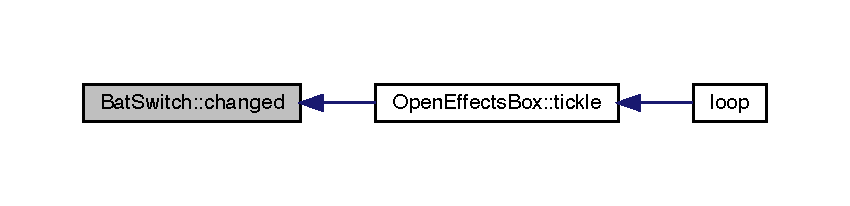
\includegraphics[width=350pt]{class_bat_switch_a4213173651fbb8c7fdcef12799318da4_icgraph}
\end{center}
\end{figure}
\mbox{\Hypertarget{class_bat_switch_af2180338890cebe52ff16427361383bd}\label{class_bat_switch_af2180338890cebe52ff16427361383bd}} 
\index{Bat\+Switch@{Bat\+Switch}!clear\+State@{clear\+State}}
\index{clear\+State@{clear\+State}!Bat\+Switch@{Bat\+Switch}}
\subsubsection{\texorpdfstring{clear\+State()}{clearState()}}
{\footnotesize\ttfamily void Bat\+Switch\+::clear\+State (\begin{DoxyParamCaption}{ }\end{DoxyParamCaption})}

\mbox{\Hypertarget{class_bat_switch_a2a41a055ec34dbc7169f3b2161e84075}\label{class_bat_switch_a2a41a055ec34dbc7169f3b2161e84075}} 
\index{Bat\+Switch@{Bat\+Switch}!get\+Value@{get\+Value}}
\index{get\+Value@{get\+Value}!Bat\+Switch@{Bat\+Switch}}
\subsubsection{\texorpdfstring{get\+Value()}{getValue()}}
{\footnotesize\ttfamily int Bat\+Switch\+::get\+Value (\begin{DoxyParamCaption}{ }\end{DoxyParamCaption})}

Here is the caller graph for this function\+:\nopagebreak
\begin{figure}[H]
\begin{center}
\leavevmode
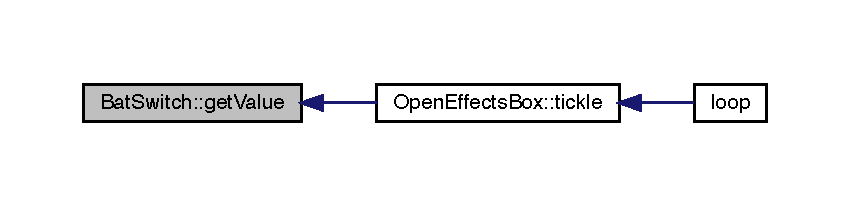
\includegraphics[width=350pt]{class_bat_switch_a2a41a055ec34dbc7169f3b2161e84075_icgraph}
\end{center}
\end{figure}
\mbox{\Hypertarget{class_bat_switch_a144b8789518472a4d5dc19f09968148e}\label{class_bat_switch_a144b8789518472a4d5dc19f09968148e}} 
\index{Bat\+Switch@{Bat\+Switch}!init@{init}}
\index{init@{init}!Bat\+Switch@{Bat\+Switch}}
\subsubsection{\texorpdfstring{init()}{init()}}
{\footnotesize\ttfamily void Bat\+Switch\+::init (\begin{DoxyParamCaption}\item[{int}]{id,  }\item[{int}]{pin }\end{DoxyParamCaption})}

Here is the caller graph for this function\+:\nopagebreak
\begin{figure}[H]
\begin{center}
\leavevmode
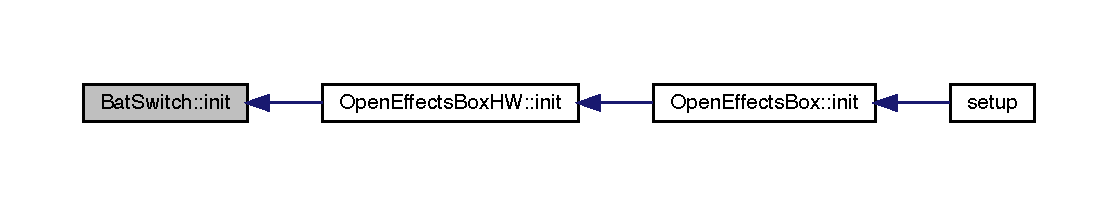
\includegraphics[width=350pt]{class_bat_switch_a144b8789518472a4d5dc19f09968148e_icgraph}
\end{center}
\end{figure}
\mbox{\Hypertarget{class_bat_switch_ac22ba354f82cc1c0e2e8d6876305ea66}\label{class_bat_switch_ac22ba354f82cc1c0e2e8d6876305ea66}} 
\index{Bat\+Switch@{Bat\+Switch}!update@{update}}
\index{update@{update}!Bat\+Switch@{Bat\+Switch}}
\subsubsection{\texorpdfstring{update()}{update()}}
{\footnotesize\ttfamily void Bat\+Switch\+::update (\begin{DoxyParamCaption}{ }\end{DoxyParamCaption})}



The documentation for this class was generated from the following files\+:\begin{DoxyCompactItemize}
\item 
\mbox{\hyperlink{_bat_switch_8h}{Bat\+Switch.\+h}}\item 
\mbox{\hyperlink{_bat_switch_8cpp}{Bat\+Switch.\+cpp}}\end{DoxyCompactItemize}

\hypertarget{class_bitcrusher}{}\section{Bitcrusher Class Reference}
\label{class_bitcrusher}\index{Bitcrusher@{Bitcrusher}}


Wrapper for Audio Design Tool -\/\+Bitcrusher-\/.  




{\ttfamily \#include $<$Bitcrusher.\+h$>$}



Inheritance diagram for Bitcrusher\+:
\nopagebreak
\begin{figure}[H]
\begin{center}
\leavevmode
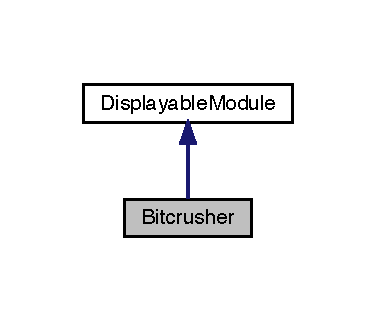
\includegraphics[width=180pt]{class_bitcrusher__inherit__graph}
\end{center}
\end{figure}


Collaboration diagram for Bitcrusher\+:
\nopagebreak
\begin{figure}[H]
\begin{center}
\leavevmode
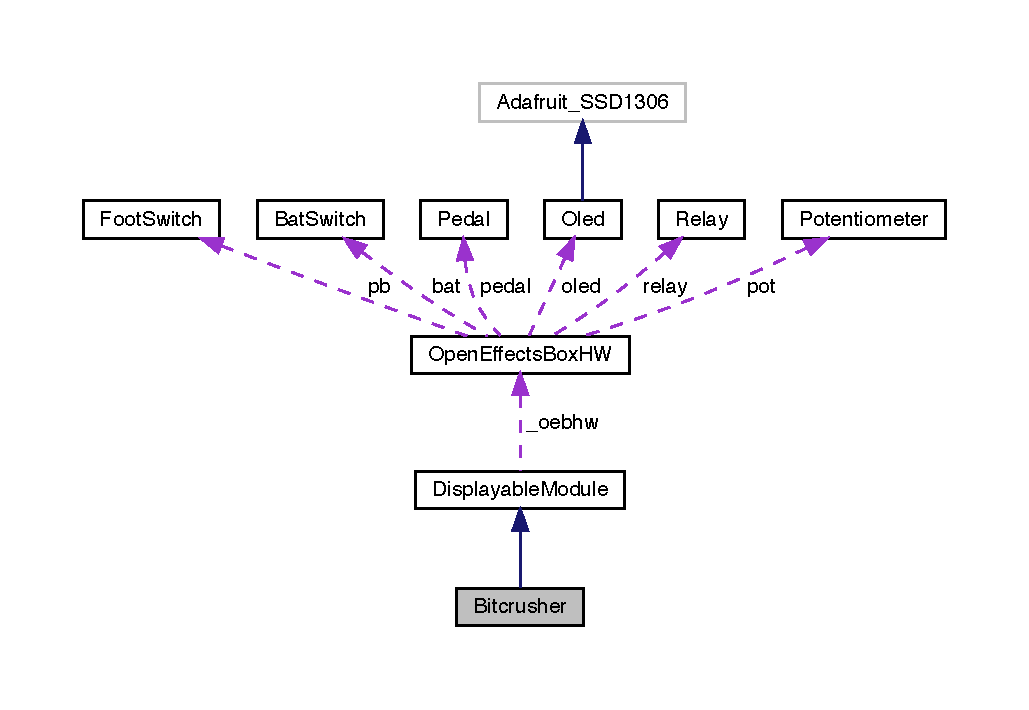
\includegraphics[width=350pt]{class_bitcrusher__coll__graph}
\end{center}
\end{figure}
\subsection*{Public Member Functions}
\begin{DoxyCompactItemize}
\item 
\mbox{\hyperlink{class_bitcrusher_ad130a5c022020a6e64ed6dc75f8d2372}{Bitcrusher}} ()
\item 
void \mbox{\hyperlink{class_bitcrusher_a2ea948d02aaeec7ef5af9dd35346d29c}{set\+Verbose}} (int verbose)
\item 
void \mbox{\hyperlink{class_bitcrusher_a8d46a549db08c6c022c55f10b348647d}{init}} (int id, char $\ast$name, Audio\+Effect\+Bitcrusher $\ast$\+\_\+bitcrusher, \mbox{\hyperlink{class_open_effects_box_h_w}{Open\+Effects\+Box\+HW}} $\ast$oebhw, int verbose=\mbox{\hyperlink{_bitcrusher_8h_a11f2932e6b24f27a8025c6bfe4e234c0}{Bitcrusher\+\_\+\+V\+E\+R\+B\+O\+S\+E\+\_\+\+D\+E\+F\+A\+U\+LT}})
\item 
void \mbox{\hyperlink{class_bitcrusher_ae392ad4b140a5121df417ece060911f4}{notify}} (int channel, float value)
\item 
void \mbox{\hyperlink{class_bitcrusher_aa5d365b3690a76f968465b9e841720f6}{display}} (int mode, int sub\+Mode, bool force=false)
\item 
void \mbox{\hyperlink{class_bitcrusher_a4c2ecf3d6fc604a9967685256a886503}{set\+N\+Bits}} (int n\+Bits)
\item 
void \mbox{\hyperlink{class_bitcrusher_a0b50f63f1b533074ef8acd41714ae1d3}{set\+Sample\+Rate}} (unsigned int sample\+Rate)
\end{DoxyCompactItemize}
\subsection*{Additional Inherited Members}


\subsection{Detailed Description}
Wrapper for Audio Design Tool -\/\+Bitcrusher-\/. 

See \href{https://www.pjrc.com/teensy/gui/}{\tt Paul Stoffregen\textquotesingle{}s Audio Design Tool} 

\subsection{Constructor \& Destructor Documentation}
\mbox{\Hypertarget{class_bitcrusher_ad130a5c022020a6e64ed6dc75f8d2372}\label{class_bitcrusher_ad130a5c022020a6e64ed6dc75f8d2372}} 
\index{Bitcrusher@{Bitcrusher}!Bitcrusher@{Bitcrusher}}
\index{Bitcrusher@{Bitcrusher}!Bitcrusher@{Bitcrusher}}
\subsubsection{\texorpdfstring{Bitcrusher()}{Bitcrusher()}}
{\footnotesize\ttfamily Bitcrusher\+::\+Bitcrusher (\begin{DoxyParamCaption}{ }\end{DoxyParamCaption})}



\subsection{Member Function Documentation}
\mbox{\Hypertarget{class_bitcrusher_aa5d365b3690a76f968465b9e841720f6}\label{class_bitcrusher_aa5d365b3690a76f968465b9e841720f6}} 
\index{Bitcrusher@{Bitcrusher}!display@{display}}
\index{display@{display}!Bitcrusher@{Bitcrusher}}
\subsubsection{\texorpdfstring{display()}{display()}}
{\footnotesize\ttfamily void Bitcrusher\+::display (\begin{DoxyParamCaption}\item[{int}]{mode,  }\item[{int}]{sub\+Mode,  }\item[{bool}]{force = {\ttfamily false} }\end{DoxyParamCaption})\hspace{0.3cm}{\ttfamily [virtual]}}



Reimplemented from \mbox{\hyperlink{class_displayable_module_a02de26d62ef508cae9ed07920e21784d}{Displayable\+Module}}.

Here is the call graph for this function\+:\nopagebreak
\begin{figure}[H]
\begin{center}
\leavevmode
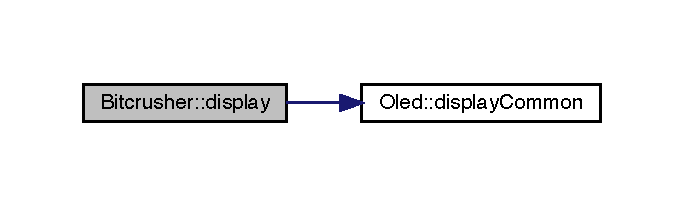
\includegraphics[width=328pt]{class_bitcrusher_aa5d365b3690a76f968465b9e841720f6_cgraph}
\end{center}
\end{figure}
\mbox{\Hypertarget{class_bitcrusher_a8d46a549db08c6c022c55f10b348647d}\label{class_bitcrusher_a8d46a549db08c6c022c55f10b348647d}} 
\index{Bitcrusher@{Bitcrusher}!init@{init}}
\index{init@{init}!Bitcrusher@{Bitcrusher}}
\subsubsection{\texorpdfstring{init()}{init()}}
{\footnotesize\ttfamily void Bitcrusher\+::init (\begin{DoxyParamCaption}\item[{int}]{id,  }\item[{char $\ast$}]{name,  }\item[{Audio\+Effect\+Bitcrusher $\ast$}]{\+\_\+bitcrusher,  }\item[{\mbox{\hyperlink{class_open_effects_box_h_w}{Open\+Effects\+Box\+HW}} $\ast$}]{oebhw,  }\item[{int}]{verbose = {\ttfamily \mbox{\hyperlink{_bitcrusher_8h_a11f2932e6b24f27a8025c6bfe4e234c0}{Bitcrusher\+\_\+\+V\+E\+R\+B\+O\+S\+E\+\_\+\+D\+E\+F\+A\+U\+LT}}} }\end{DoxyParamCaption})}

Here is the call graph for this function\+:\nopagebreak
\begin{figure}[H]
\begin{center}
\leavevmode
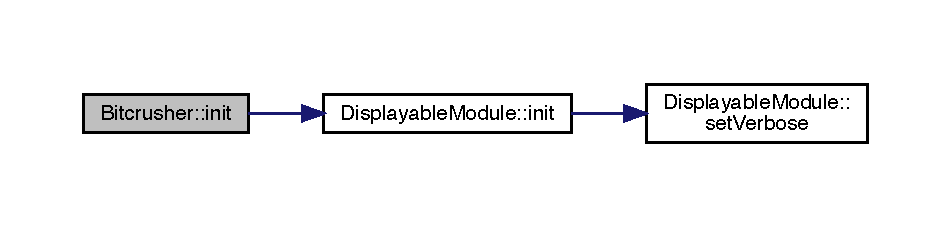
\includegraphics[width=350pt]{class_bitcrusher_a8d46a549db08c6c022c55f10b348647d_cgraph}
\end{center}
\end{figure}
Here is the caller graph for this function\+:\nopagebreak
\begin{figure}[H]
\begin{center}
\leavevmode
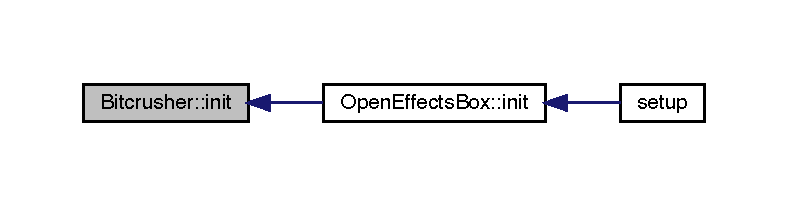
\includegraphics[width=350pt]{class_bitcrusher_a8d46a549db08c6c022c55f10b348647d_icgraph}
\end{center}
\end{figure}
\mbox{\Hypertarget{class_bitcrusher_ae392ad4b140a5121df417ece060911f4}\label{class_bitcrusher_ae392ad4b140a5121df417ece060911f4}} 
\index{Bitcrusher@{Bitcrusher}!notify@{notify}}
\index{notify@{notify}!Bitcrusher@{Bitcrusher}}
\subsubsection{\texorpdfstring{notify()}{notify()}}
{\footnotesize\ttfamily void Bitcrusher\+::notify (\begin{DoxyParamCaption}\item[{int}]{channel,  }\item[{float}]{value }\end{DoxyParamCaption})\hspace{0.3cm}{\ttfamily [virtual]}}



Reimplemented from \mbox{\hyperlink{class_displayable_module_a8ae5383931f10c54cff2feef2bc07dee}{Displayable\+Module}}.

Here is the call graph for this function\+:\nopagebreak
\begin{figure}[H]
\begin{center}
\leavevmode
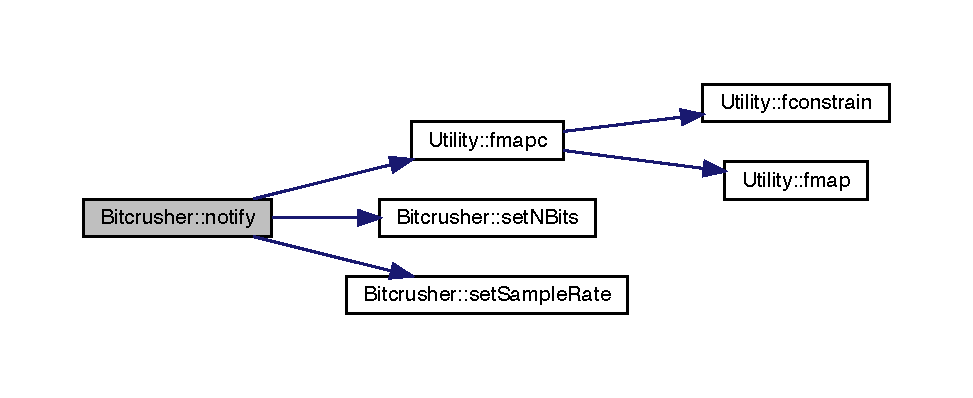
\includegraphics[width=350pt]{class_bitcrusher_ae392ad4b140a5121df417ece060911f4_cgraph}
\end{center}
\end{figure}
\mbox{\Hypertarget{class_bitcrusher_a4c2ecf3d6fc604a9967685256a886503}\label{class_bitcrusher_a4c2ecf3d6fc604a9967685256a886503}} 
\index{Bitcrusher@{Bitcrusher}!set\+N\+Bits@{set\+N\+Bits}}
\index{set\+N\+Bits@{set\+N\+Bits}!Bitcrusher@{Bitcrusher}}
\subsubsection{\texorpdfstring{set\+N\+Bits()}{setNBits()}}
{\footnotesize\ttfamily void Bitcrusher\+::set\+N\+Bits (\begin{DoxyParamCaption}\item[{int}]{n\+Bits }\end{DoxyParamCaption})}

Here is the caller graph for this function\+:\nopagebreak
\begin{figure}[H]
\begin{center}
\leavevmode
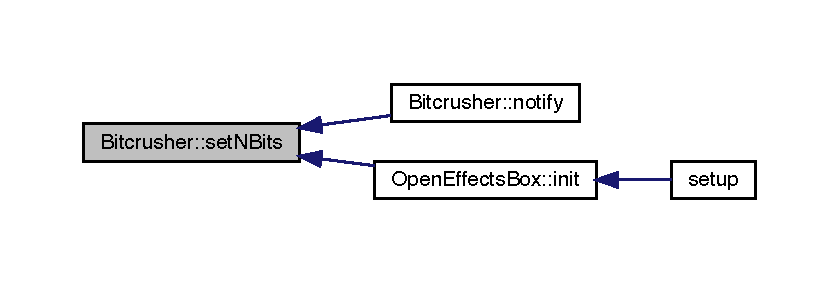
\includegraphics[width=350pt]{class_bitcrusher_a4c2ecf3d6fc604a9967685256a886503_icgraph}
\end{center}
\end{figure}
\mbox{\Hypertarget{class_bitcrusher_a0b50f63f1b533074ef8acd41714ae1d3}\label{class_bitcrusher_a0b50f63f1b533074ef8acd41714ae1d3}} 
\index{Bitcrusher@{Bitcrusher}!set\+Sample\+Rate@{set\+Sample\+Rate}}
\index{set\+Sample\+Rate@{set\+Sample\+Rate}!Bitcrusher@{Bitcrusher}}
\subsubsection{\texorpdfstring{set\+Sample\+Rate()}{setSampleRate()}}
{\footnotesize\ttfamily void Bitcrusher\+::set\+Sample\+Rate (\begin{DoxyParamCaption}\item[{unsigned int}]{sample\+Rate }\end{DoxyParamCaption})}

Here is the caller graph for this function\+:\nopagebreak
\begin{figure}[H]
\begin{center}
\leavevmode
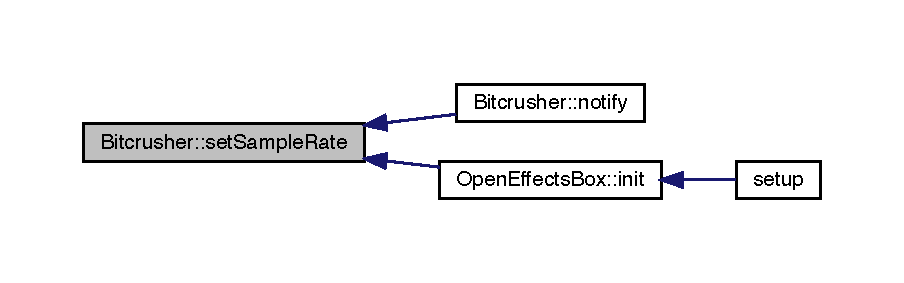
\includegraphics[width=350pt]{class_bitcrusher_a0b50f63f1b533074ef8acd41714ae1d3_icgraph}
\end{center}
\end{figure}
\mbox{\Hypertarget{class_bitcrusher_a2ea948d02aaeec7ef5af9dd35346d29c}\label{class_bitcrusher_a2ea948d02aaeec7ef5af9dd35346d29c}} 
\index{Bitcrusher@{Bitcrusher}!set\+Verbose@{set\+Verbose}}
\index{set\+Verbose@{set\+Verbose}!Bitcrusher@{Bitcrusher}}
\subsubsection{\texorpdfstring{set\+Verbose()}{setVerbose()}}
{\footnotesize\ttfamily void Bitcrusher\+::set\+Verbose (\begin{DoxyParamCaption}\item[{int}]{verbose }\end{DoxyParamCaption})}



The documentation for this class was generated from the following files\+:\begin{DoxyCompactItemize}
\item 
\mbox{\hyperlink{_bitcrusher_8h}{Bitcrusher.\+h}}\item 
\mbox{\hyperlink{_bitcrusher_8cpp}{Bitcrusher.\+cpp}}\end{DoxyCompactItemize}

\hypertarget{class_chorus}{}\section{Chorus Class Reference}
\label{class_chorus}\index{Chorus@{Chorus}}


Wrapper for Audio Design Tool -\/\+Chorus-\/.  




{\ttfamily \#include $<$Chorus.\+h$>$}



Inheritance diagram for Chorus\+:
\nopagebreak
\begin{figure}[H]
\begin{center}
\leavevmode
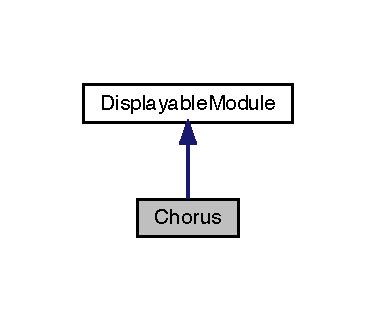
\includegraphics[width=180pt]{class_chorus__inherit__graph}
\end{center}
\end{figure}


Collaboration diagram for Chorus\+:
\nopagebreak
\begin{figure}[H]
\begin{center}
\leavevmode
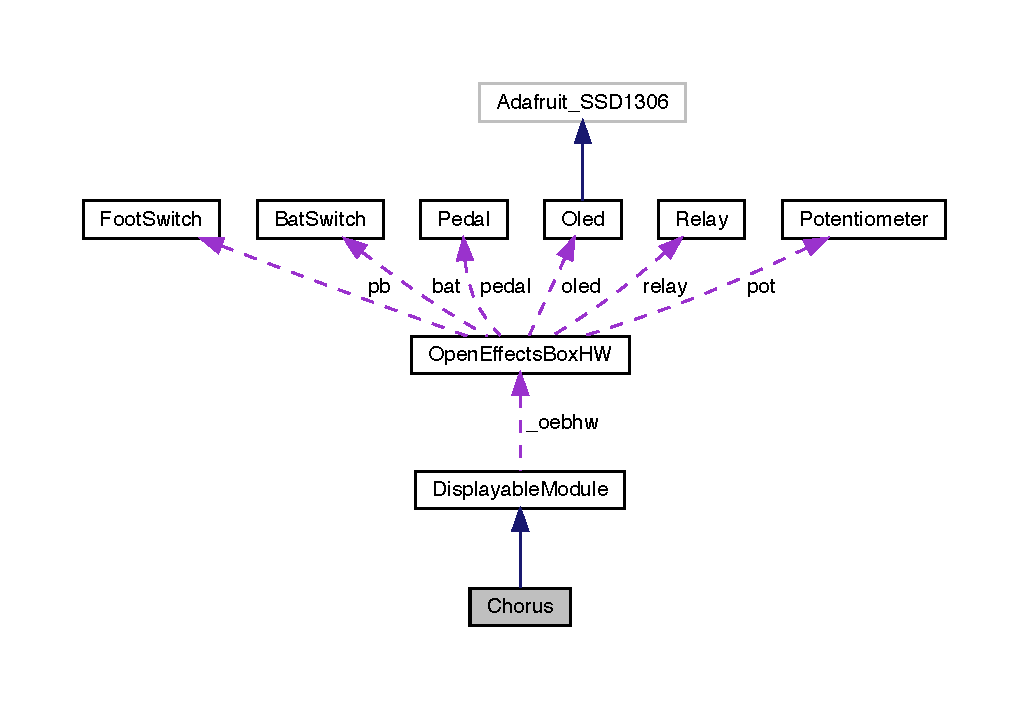
\includegraphics[width=350pt]{class_chorus__coll__graph}
\end{center}
\end{figure}
\subsection*{Public Member Functions}
\begin{DoxyCompactItemize}
\item 
\mbox{\hyperlink{class_chorus_a125a7aa1daf841c2da11450b0c79b51b}{Chorus}} ()
\item 
void \mbox{\hyperlink{class_chorus_a26bc317aad64c5da7b643e57178b3e89}{set\+Verbose}} (int verbose)
\item 
void \mbox{\hyperlink{class_chorus_a234b46541693909b60a21cf644bd5926}{init}} (int id, char $\ast$name, Audio\+Effect\+Chorus $\ast$chorus, \mbox{\hyperlink{class_open_effects_box_h_w}{Open\+Effects\+Box\+HW}} $\ast$oebhw, int verbose=\mbox{\hyperlink{_chorus_8h_ab3779d2226e8ab06fa78da0c6161597a}{Chorus\+\_\+\+V\+E\+R\+B\+O\+S\+E\+\_\+\+D\+E\+F\+A\+U\+LT}})
\item 
void \mbox{\hyperlink{class_chorus_acb22e9cc93011859d1ae02b05a7388f5}{notify}} (int channel, float value)
\item 
void \mbox{\hyperlink{class_chorus_a6a28900025c58af59c7eb70f49347422}{display}} (int mode, int sub\+Mode, bool force=false)
\item 
void \mbox{\hyperlink{class_chorus_adfe582e095779c9a658a9633bad8251b}{set\+N\+Voices}} (int n\+Voices)
\end{DoxyCompactItemize}
\subsection*{Additional Inherited Members}


\subsection{Detailed Description}
Wrapper for Audio Design Tool -\/\+Chorus-\/. 

See \href{https://www.pjrc.com/teensy/gui/}{\tt Paul Stoffregen\textquotesingle{}s Audio Design Tool} 

\subsection{Constructor \& Destructor Documentation}
\mbox{\Hypertarget{class_chorus_a125a7aa1daf841c2da11450b0c79b51b}\label{class_chorus_a125a7aa1daf841c2da11450b0c79b51b}} 
\index{Chorus@{Chorus}!Chorus@{Chorus}}
\index{Chorus@{Chorus}!Chorus@{Chorus}}
\subsubsection{\texorpdfstring{Chorus()}{Chorus()}}
{\footnotesize\ttfamily Chorus\+::\+Chorus (\begin{DoxyParamCaption}{ }\end{DoxyParamCaption})}



\subsection{Member Function Documentation}
\mbox{\Hypertarget{class_chorus_a6a28900025c58af59c7eb70f49347422}\label{class_chorus_a6a28900025c58af59c7eb70f49347422}} 
\index{Chorus@{Chorus}!display@{display}}
\index{display@{display}!Chorus@{Chorus}}
\subsubsection{\texorpdfstring{display()}{display()}}
{\footnotesize\ttfamily void Chorus\+::display (\begin{DoxyParamCaption}\item[{int}]{mode,  }\item[{int}]{sub\+Mode,  }\item[{bool}]{force = {\ttfamily false} }\end{DoxyParamCaption})\hspace{0.3cm}{\ttfamily [virtual]}}



Reimplemented from \mbox{\hyperlink{class_displayable_module_a02de26d62ef508cae9ed07920e21784d}{Displayable\+Module}}.

Here is the call graph for this function\+:\nopagebreak
\begin{figure}[H]
\begin{center}
\leavevmode
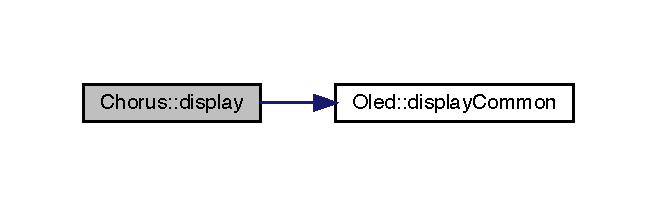
\includegraphics[width=315pt]{class_chorus_a6a28900025c58af59c7eb70f49347422_cgraph}
\end{center}
\end{figure}
\mbox{\Hypertarget{class_chorus_a234b46541693909b60a21cf644bd5926}\label{class_chorus_a234b46541693909b60a21cf644bd5926}} 
\index{Chorus@{Chorus}!init@{init}}
\index{init@{init}!Chorus@{Chorus}}
\subsubsection{\texorpdfstring{init()}{init()}}
{\footnotesize\ttfamily void Chorus\+::init (\begin{DoxyParamCaption}\item[{int}]{id,  }\item[{char $\ast$}]{name,  }\item[{Audio\+Effect\+Chorus $\ast$}]{chorus,  }\item[{\mbox{\hyperlink{class_open_effects_box_h_w}{Open\+Effects\+Box\+HW}} $\ast$}]{oebhw,  }\item[{int}]{verbose = {\ttfamily \mbox{\hyperlink{_chorus_8h_ab3779d2226e8ab06fa78da0c6161597a}{Chorus\+\_\+\+V\+E\+R\+B\+O\+S\+E\+\_\+\+D\+E\+F\+A\+U\+LT}}} }\end{DoxyParamCaption})}

Here is the call graph for this function\+:\nopagebreak
\begin{figure}[H]
\begin{center}
\leavevmode
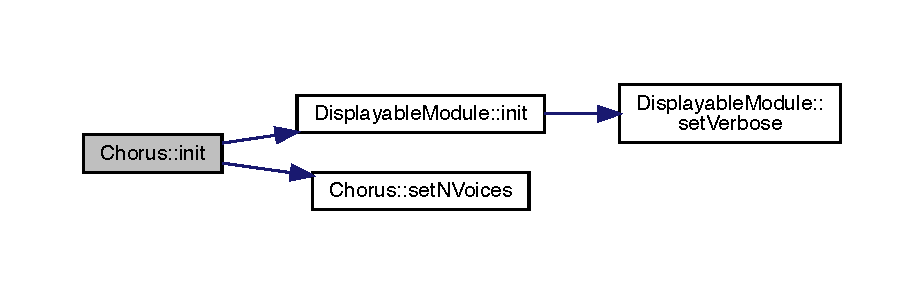
\includegraphics[width=350pt]{class_chorus_a234b46541693909b60a21cf644bd5926_cgraph}
\end{center}
\end{figure}
Here is the caller graph for this function\+:\nopagebreak
\begin{figure}[H]
\begin{center}
\leavevmode
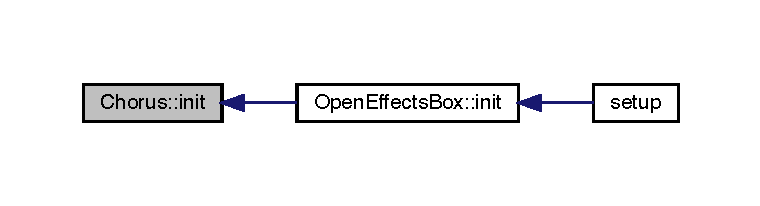
\includegraphics[width=350pt]{class_chorus_a234b46541693909b60a21cf644bd5926_icgraph}
\end{center}
\end{figure}
\mbox{\Hypertarget{class_chorus_acb22e9cc93011859d1ae02b05a7388f5}\label{class_chorus_acb22e9cc93011859d1ae02b05a7388f5}} 
\index{Chorus@{Chorus}!notify@{notify}}
\index{notify@{notify}!Chorus@{Chorus}}
\subsubsection{\texorpdfstring{notify()}{notify()}}
{\footnotesize\ttfamily void Chorus\+::notify (\begin{DoxyParamCaption}\item[{int}]{channel,  }\item[{float}]{value }\end{DoxyParamCaption})\hspace{0.3cm}{\ttfamily [virtual]}}



Reimplemented from \mbox{\hyperlink{class_displayable_module_a8ae5383931f10c54cff2feef2bc07dee}{Displayable\+Module}}.

Here is the call graph for this function\+:\nopagebreak
\begin{figure}[H]
\begin{center}
\leavevmode
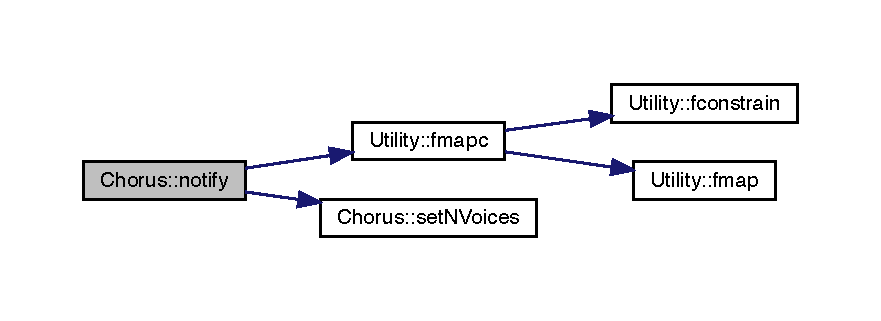
\includegraphics[width=350pt]{class_chorus_acb22e9cc93011859d1ae02b05a7388f5_cgraph}
\end{center}
\end{figure}
\mbox{\Hypertarget{class_chorus_adfe582e095779c9a658a9633bad8251b}\label{class_chorus_adfe582e095779c9a658a9633bad8251b}} 
\index{Chorus@{Chorus}!set\+N\+Voices@{set\+N\+Voices}}
\index{set\+N\+Voices@{set\+N\+Voices}!Chorus@{Chorus}}
\subsubsection{\texorpdfstring{set\+N\+Voices()}{setNVoices()}}
{\footnotesize\ttfamily void Chorus\+::set\+N\+Voices (\begin{DoxyParamCaption}\item[{int}]{n\+Voices }\end{DoxyParamCaption})}

Here is the caller graph for this function\+:\nopagebreak
\begin{figure}[H]
\begin{center}
\leavevmode
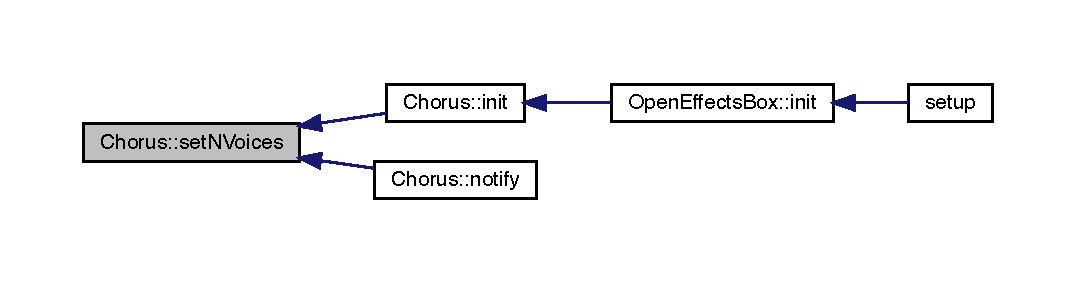
\includegraphics[width=350pt]{class_chorus_adfe582e095779c9a658a9633bad8251b_icgraph}
\end{center}
\end{figure}
\mbox{\Hypertarget{class_chorus_a26bc317aad64c5da7b643e57178b3e89}\label{class_chorus_a26bc317aad64c5da7b643e57178b3e89}} 
\index{Chorus@{Chorus}!set\+Verbose@{set\+Verbose}}
\index{set\+Verbose@{set\+Verbose}!Chorus@{Chorus}}
\subsubsection{\texorpdfstring{set\+Verbose()}{setVerbose()}}
{\footnotesize\ttfamily void Chorus\+::set\+Verbose (\begin{DoxyParamCaption}\item[{int}]{verbose }\end{DoxyParamCaption})}



The documentation for this class was generated from the following files\+:\begin{DoxyCompactItemize}
\item 
\mbox{\hyperlink{_chorus_8h}{Chorus.\+h}}\item 
\mbox{\hyperlink{_chorus_8cpp}{Chorus.\+cpp}}\end{DoxyCompactItemize}

\hypertarget{class_d_c}{}\section{DC Class Reference}
\label{class_d_c}\index{DC@{DC}}


Wrapper for Audio Design Tool -\/\+D\+C-\/.  




{\ttfamily \#include $<$D\+C.\+h$>$}



Inheritance diagram for DC\+:
\nopagebreak
\begin{figure}[H]
\begin{center}
\leavevmode
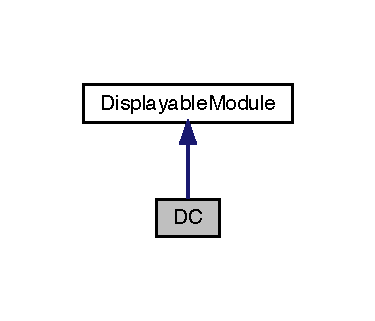
\includegraphics[width=180pt]{class_d_c__inherit__graph}
\end{center}
\end{figure}


Collaboration diagram for DC\+:
\nopagebreak
\begin{figure}[H]
\begin{center}
\leavevmode
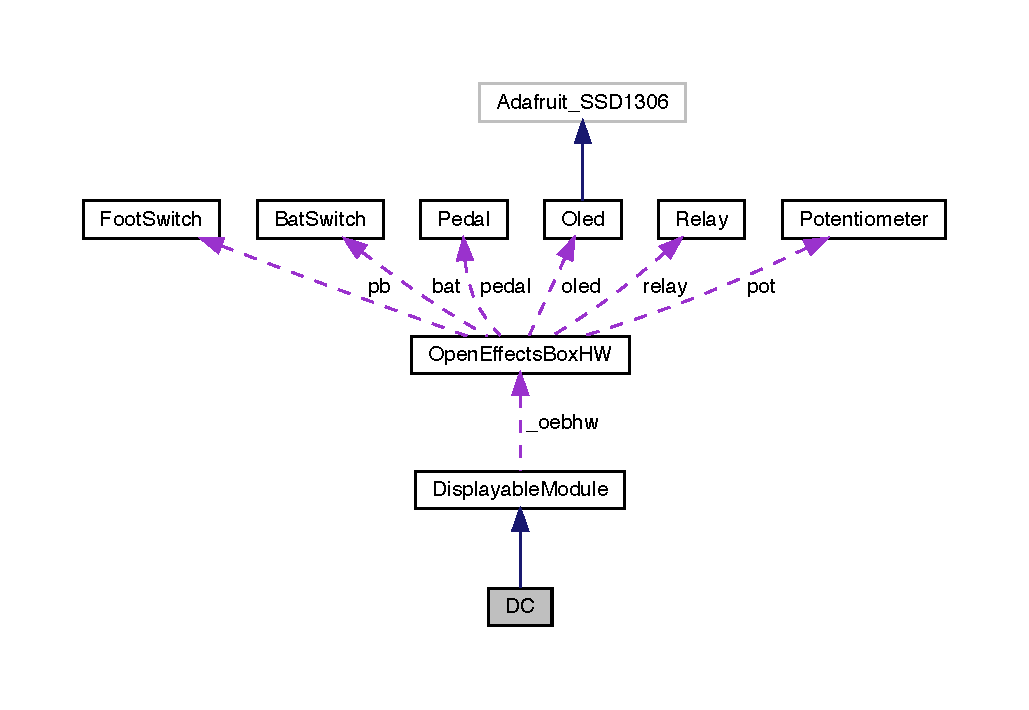
\includegraphics[width=350pt]{class_d_c__coll__graph}
\end{center}
\end{figure}
\subsection*{Public Member Functions}
\begin{DoxyCompactItemize}
\item 
\mbox{\hyperlink{class_d_c_a921648df43516afc9b7ffa044ce6f4a8}{DC}} ()
\item 
void \mbox{\hyperlink{class_d_c_a1fb27467a4ab9013b6b01fb6295ada42}{set\+Verbose}} (int verbose)
\item 
void \mbox{\hyperlink{class_d_c_a767b3f22587703e7f59020d44872f432}{init}} (int id, char $\ast$name, Audio\+Synth\+Waveform\+Dc $\ast$dc, \mbox{\hyperlink{class_open_effects_box_h_w}{Open\+Effects\+Box\+HW}} $\ast$oebhw, int verbose=\mbox{\hyperlink{_d_c_8h_a41fb888bc7c99c6ae3c43304971faeb6}{D\+C\+\_\+\+V\+E\+R\+B\+O\+S\+E\+\_\+\+D\+E\+F\+A\+U\+LT}})
\item 
void \mbox{\hyperlink{class_d_c_a45e51132fbd69668134f3ab13f3668b1}{notify}} (int channel, float value)
\item 
void \mbox{\hyperlink{class_d_c_a006f266e63bdff5042fa2c443e1a04cc}{display}} (int mode, int sub\+Mode, bool force=false)
\item 
void \mbox{\hyperlink{class_d_c_aa7f1c23c91d43443c018cc48ab6db5ef}{set\+Level}} (float level)
\end{DoxyCompactItemize}
\subsection*{Additional Inherited Members}


\subsection{Detailed Description}
Wrapper for Audio Design Tool -\/\+D\+C-\/. 

See \href{https://www.pjrc.com/teensy/gui/}{\tt Paul Stoffregen\textquotesingle{}s Audio Design Tool} 

\subsection{Constructor \& Destructor Documentation}
\mbox{\Hypertarget{class_d_c_a921648df43516afc9b7ffa044ce6f4a8}\label{class_d_c_a921648df43516afc9b7ffa044ce6f4a8}} 
\index{DC@{DC}!DC@{DC}}
\index{DC@{DC}!DC@{DC}}
\subsubsection{\texorpdfstring{D\+C()}{DC()}}
{\footnotesize\ttfamily D\+C\+::\+DC (\begin{DoxyParamCaption}{ }\end{DoxyParamCaption})}



\subsection{Member Function Documentation}
\mbox{\Hypertarget{class_d_c_a006f266e63bdff5042fa2c443e1a04cc}\label{class_d_c_a006f266e63bdff5042fa2c443e1a04cc}} 
\index{DC@{DC}!display@{display}}
\index{display@{display}!DC@{DC}}
\subsubsection{\texorpdfstring{display()}{display()}}
{\footnotesize\ttfamily void D\+C\+::display (\begin{DoxyParamCaption}\item[{int}]{mode,  }\item[{int}]{sub\+Mode,  }\item[{bool}]{force = {\ttfamily false} }\end{DoxyParamCaption})\hspace{0.3cm}{\ttfamily [virtual]}}



Reimplemented from \mbox{\hyperlink{class_displayable_module_a02de26d62ef508cae9ed07920e21784d}{Displayable\+Module}}.

Here is the call graph for this function\+:\nopagebreak
\begin{figure}[H]
\begin{center}
\leavevmode
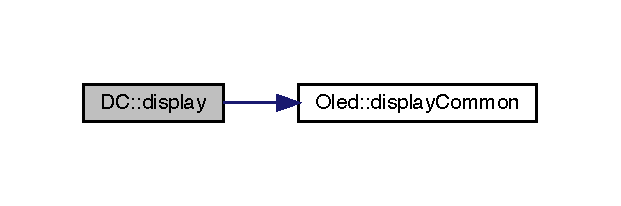
\includegraphics[width=298pt]{class_d_c_a006f266e63bdff5042fa2c443e1a04cc_cgraph}
\end{center}
\end{figure}
\mbox{\Hypertarget{class_d_c_a767b3f22587703e7f59020d44872f432}\label{class_d_c_a767b3f22587703e7f59020d44872f432}} 
\index{DC@{DC}!init@{init}}
\index{init@{init}!DC@{DC}}
\subsubsection{\texorpdfstring{init()}{init()}}
{\footnotesize\ttfamily void D\+C\+::init (\begin{DoxyParamCaption}\item[{int}]{id,  }\item[{char $\ast$}]{name,  }\item[{Audio\+Synth\+Waveform\+Dc $\ast$}]{dc,  }\item[{\mbox{\hyperlink{class_open_effects_box_h_w}{Open\+Effects\+Box\+HW}} $\ast$}]{oebhw,  }\item[{int}]{verbose = {\ttfamily \mbox{\hyperlink{_d_c_8h_a41fb888bc7c99c6ae3c43304971faeb6}{D\+C\+\_\+\+V\+E\+R\+B\+O\+S\+E\+\_\+\+D\+E\+F\+A\+U\+LT}}} }\end{DoxyParamCaption})}

Here is the call graph for this function\+:\nopagebreak
\begin{figure}[H]
\begin{center}
\leavevmode
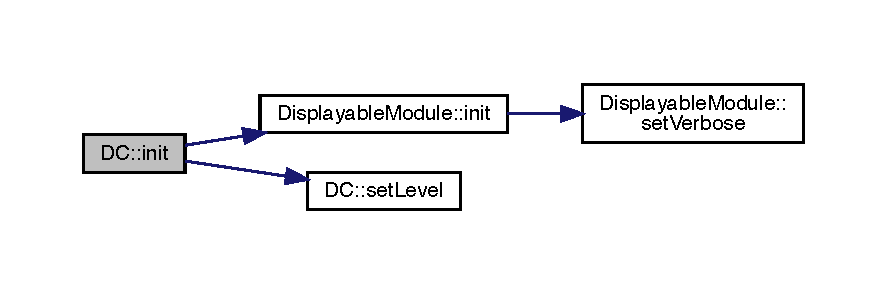
\includegraphics[width=350pt]{class_d_c_a767b3f22587703e7f59020d44872f432_cgraph}
\end{center}
\end{figure}
Here is the caller graph for this function\+:\nopagebreak
\begin{figure}[H]
\begin{center}
\leavevmode
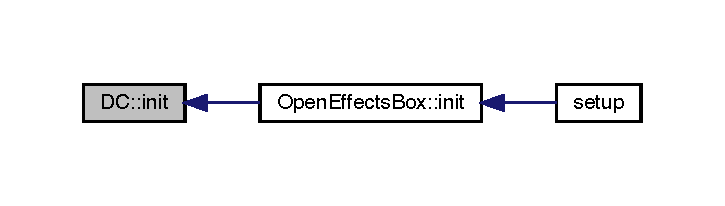
\includegraphics[width=348pt]{class_d_c_a767b3f22587703e7f59020d44872f432_icgraph}
\end{center}
\end{figure}
\mbox{\Hypertarget{class_d_c_a45e51132fbd69668134f3ab13f3668b1}\label{class_d_c_a45e51132fbd69668134f3ab13f3668b1}} 
\index{DC@{DC}!notify@{notify}}
\index{notify@{notify}!DC@{DC}}
\subsubsection{\texorpdfstring{notify()}{notify()}}
{\footnotesize\ttfamily void D\+C\+::notify (\begin{DoxyParamCaption}\item[{int}]{channel,  }\item[{float}]{value }\end{DoxyParamCaption})\hspace{0.3cm}{\ttfamily [virtual]}}



Reimplemented from \mbox{\hyperlink{class_displayable_module_a8ae5383931f10c54cff2feef2bc07dee}{Displayable\+Module}}.

Here is the call graph for this function\+:\nopagebreak
\begin{figure}[H]
\begin{center}
\leavevmode
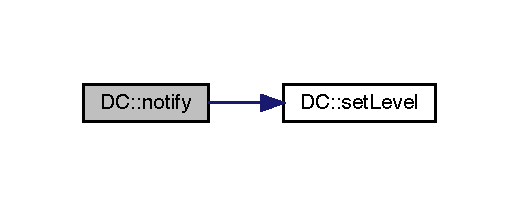
\includegraphics[width=249pt]{class_d_c_a45e51132fbd69668134f3ab13f3668b1_cgraph}
\end{center}
\end{figure}
\mbox{\Hypertarget{class_d_c_aa7f1c23c91d43443c018cc48ab6db5ef}\label{class_d_c_aa7f1c23c91d43443c018cc48ab6db5ef}} 
\index{DC@{DC}!set\+Level@{set\+Level}}
\index{set\+Level@{set\+Level}!DC@{DC}}
\subsubsection{\texorpdfstring{set\+Level()}{setLevel()}}
{\footnotesize\ttfamily void D\+C\+::set\+Level (\begin{DoxyParamCaption}\item[{float}]{level }\end{DoxyParamCaption})}

Here is the caller graph for this function\+:\nopagebreak
\begin{figure}[H]
\begin{center}
\leavevmode
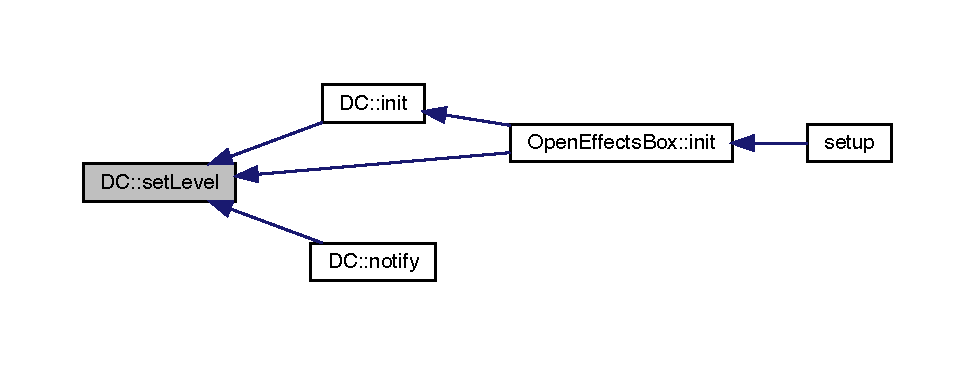
\includegraphics[width=350pt]{class_d_c_aa7f1c23c91d43443c018cc48ab6db5ef_icgraph}
\end{center}
\end{figure}
\mbox{\Hypertarget{class_d_c_a1fb27467a4ab9013b6b01fb6295ada42}\label{class_d_c_a1fb27467a4ab9013b6b01fb6295ada42}} 
\index{DC@{DC}!set\+Verbose@{set\+Verbose}}
\index{set\+Verbose@{set\+Verbose}!DC@{DC}}
\subsubsection{\texorpdfstring{set\+Verbose()}{setVerbose()}}
{\footnotesize\ttfamily void D\+C\+::set\+Verbose (\begin{DoxyParamCaption}\item[{int}]{verbose }\end{DoxyParamCaption})}



The documentation for this class was generated from the following files\+:\begin{DoxyCompactItemize}
\item 
\mbox{\hyperlink{_d_c_8h}{D\+C.\+h}}\item 
\mbox{\hyperlink{_d_c_8cpp}{D\+C.\+cpp}}\end{DoxyCompactItemize}

\hypertarget{class_delay_ext}{}\section{Delay\+Ext Class Reference}
\label{class_delay_ext}\index{Delay\+Ext@{Delay\+Ext}}


Wrapper for Audio Design Tool -\/\+Reverb-\/.  




{\ttfamily \#include $<$Delay\+Ext.\+h$>$}



Inheritance diagram for Delay\+Ext\+:
\nopagebreak
\begin{figure}[H]
\begin{center}
\leavevmode
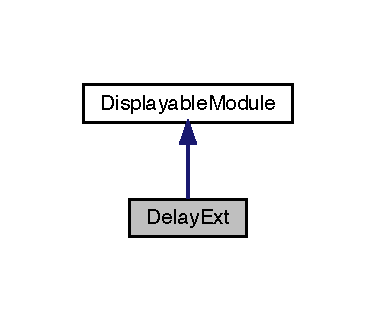
\includegraphics[width=180pt]{class_delay_ext__inherit__graph}
\end{center}
\end{figure}


Collaboration diagram for Delay\+Ext\+:
\nopagebreak
\begin{figure}[H]
\begin{center}
\leavevmode
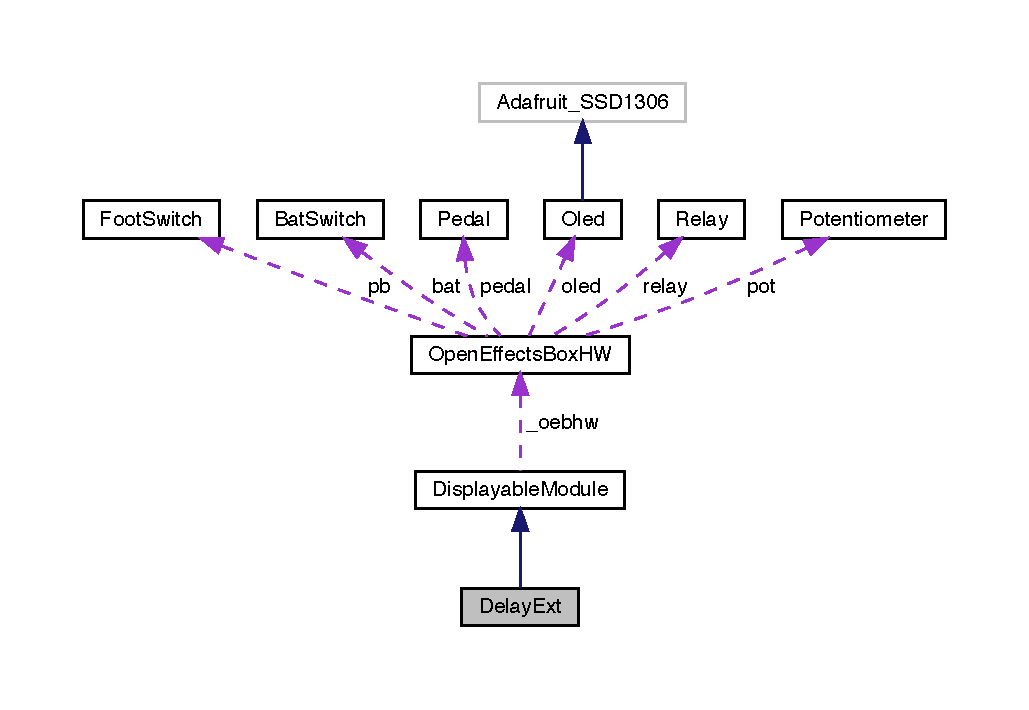
\includegraphics[width=350pt]{class_delay_ext__coll__graph}
\end{center}
\end{figure}
\subsection*{Public Member Functions}
\begin{DoxyCompactItemize}
\item 
\mbox{\hyperlink{class_delay_ext_ad0b56c7a3db3c36dc02ac08ff59ca809}{Delay\+Ext}} ()
\item 
void \mbox{\hyperlink{class_delay_ext_aced3df43297e5f6092fc2a652ab712d2}{set\+Verbose}} (int verbose)
\item 
void \mbox{\hyperlink{class_delay_ext_ac1e47f4764e44f0a623687c7a2a95e6f}{init}} (int id, char $\ast$name, Audio\+Effect\+Delay\+External $\ast$delay\+Ext, \mbox{\hyperlink{class_open_effects_box_h_w}{Open\+Effects\+Box\+HW}} $\ast$oebhw, int verbose=\mbox{\hyperlink{_delay_ext_8h_a1c2b9cd031a3baecf2c7d96325dcb9b1}{Delay\+Ext\+\_\+\+V\+E\+R\+B\+O\+S\+E\+\_\+\+D\+E\+F\+A\+U\+LT}})
\item 
void \mbox{\hyperlink{class_delay_ext_aa7e84d74c1080b5473a7401a5042b305}{init}} (int id, char $\ast$name, Audio\+Effect\+Delay\+External $\ast$delay\+Ext, \mbox{\hyperlink{class_open_effects_box_h_w}{Open\+Effects\+Box\+HW}} $\ast$oebhw, int ch0, int ch1, int ch2, int ch3, int verbose=\mbox{\hyperlink{_delay_ext_8h_a1c2b9cd031a3baecf2c7d96325dcb9b1}{Delay\+Ext\+\_\+\+V\+E\+R\+B\+O\+S\+E\+\_\+\+D\+E\+F\+A\+U\+LT}})
\item 
void \mbox{\hyperlink{class_delay_ext_a76001b2a3aad7ce1a2e1220ab7387be4}{notify}} (int channel, float value)
\item 
void \mbox{\hyperlink{class_delay_ext_a53d22982c98ab7cc1206744304ecd5a9}{display}} (int mode, int sub\+Mode, bool force=false)
\item 
void \mbox{\hyperlink{class_delay_ext_a8b6e5eca2cdca8ea83a71cf57bec96dc}{set\+Delay}} (int channel, int delay\+\_\+ms)
\end{DoxyCompactItemize}
\subsection*{Additional Inherited Members}


\subsection{Detailed Description}
Wrapper for Audio Design Tool -\/\+Reverb-\/. 

See \href{https://www.pjrc.com/teensy/gui/}{\tt Paul Stoffregen\textquotesingle{}s Audio Design Tool}

I have added a 23\+L\+C1024 memory chip to the Open\+Effects Project hardware board where provision was made for it by Øyvind Mjanger, the developer of the project. This chip allows for up to 1 1/2 seconds of delay to be added to the input signal, in each of 8 parallel channels. I\textquotesingle{}ve programmed only four of these. 

\subsection{Constructor \& Destructor Documentation}
\mbox{\Hypertarget{class_delay_ext_ad0b56c7a3db3c36dc02ac08ff59ca809}\label{class_delay_ext_ad0b56c7a3db3c36dc02ac08ff59ca809}} 
\index{Delay\+Ext@{Delay\+Ext}!Delay\+Ext@{Delay\+Ext}}
\index{Delay\+Ext@{Delay\+Ext}!Delay\+Ext@{Delay\+Ext}}
\subsubsection{\texorpdfstring{Delay\+Ext()}{DelayExt()}}
{\footnotesize\ttfamily Delay\+Ext\+::\+Delay\+Ext (\begin{DoxyParamCaption}{ }\end{DoxyParamCaption})}



\subsection{Member Function Documentation}
\mbox{\Hypertarget{class_delay_ext_a53d22982c98ab7cc1206744304ecd5a9}\label{class_delay_ext_a53d22982c98ab7cc1206744304ecd5a9}} 
\index{Delay\+Ext@{Delay\+Ext}!display@{display}}
\index{display@{display}!Delay\+Ext@{Delay\+Ext}}
\subsubsection{\texorpdfstring{display()}{display()}}
{\footnotesize\ttfamily void Delay\+Ext\+::display (\begin{DoxyParamCaption}\item[{int}]{mode,  }\item[{int}]{sub\+Mode,  }\item[{bool}]{force = {\ttfamily false} }\end{DoxyParamCaption})\hspace{0.3cm}{\ttfamily [virtual]}}



Reimplemented from \mbox{\hyperlink{class_displayable_module_a02de26d62ef508cae9ed07920e21784d}{Displayable\+Module}}.

Here is the call graph for this function\+:\nopagebreak
\begin{figure}[H]
\begin{center}
\leavevmode
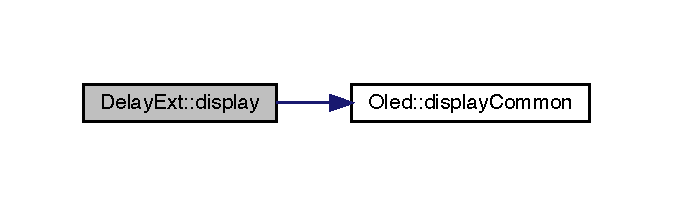
\includegraphics[width=323pt]{class_delay_ext_a53d22982c98ab7cc1206744304ecd5a9_cgraph}
\end{center}
\end{figure}
\mbox{\Hypertarget{class_delay_ext_ac1e47f4764e44f0a623687c7a2a95e6f}\label{class_delay_ext_ac1e47f4764e44f0a623687c7a2a95e6f}} 
\index{Delay\+Ext@{Delay\+Ext}!init@{init}}
\index{init@{init}!Delay\+Ext@{Delay\+Ext}}
\subsubsection{\texorpdfstring{init()}{init()}\hspace{0.1cm}{\footnotesize\ttfamily [1/2]}}
{\footnotesize\ttfamily void Delay\+Ext\+::init (\begin{DoxyParamCaption}\item[{int}]{id,  }\item[{char $\ast$}]{name,  }\item[{Audio\+Effect\+Delay\+External $\ast$}]{delay\+Ext,  }\item[{\mbox{\hyperlink{class_open_effects_box_h_w}{Open\+Effects\+Box\+HW}} $\ast$}]{oebhw,  }\item[{int}]{verbose = {\ttfamily \mbox{\hyperlink{_delay_ext_8h_a1c2b9cd031a3baecf2c7d96325dcb9b1}{Delay\+Ext\+\_\+\+V\+E\+R\+B\+O\+S\+E\+\_\+\+D\+E\+F\+A\+U\+LT}}} }\end{DoxyParamCaption})}

Here is the caller graph for this function\+:\nopagebreak
\begin{figure}[H]
\begin{center}
\leavevmode
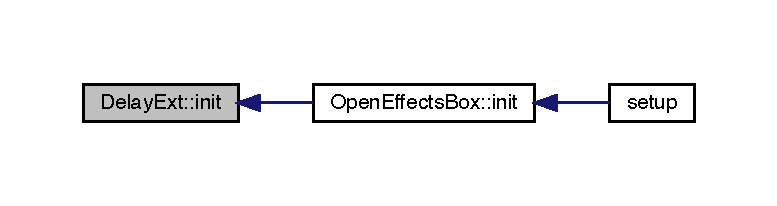
\includegraphics[width=350pt]{class_delay_ext_ac1e47f4764e44f0a623687c7a2a95e6f_icgraph}
\end{center}
\end{figure}
\mbox{\Hypertarget{class_delay_ext_aa7e84d74c1080b5473a7401a5042b305}\label{class_delay_ext_aa7e84d74c1080b5473a7401a5042b305}} 
\index{Delay\+Ext@{Delay\+Ext}!init@{init}}
\index{init@{init}!Delay\+Ext@{Delay\+Ext}}
\subsubsection{\texorpdfstring{init()}{init()}\hspace{0.1cm}{\footnotesize\ttfamily [2/2]}}
{\footnotesize\ttfamily void Delay\+Ext\+::init (\begin{DoxyParamCaption}\item[{int}]{id,  }\item[{char $\ast$}]{name,  }\item[{Audio\+Effect\+Delay\+External $\ast$}]{delay\+Ext,  }\item[{\mbox{\hyperlink{class_open_effects_box_h_w}{Open\+Effects\+Box\+HW}} $\ast$}]{oebhw,  }\item[{int}]{ch0,  }\item[{int}]{ch1,  }\item[{int}]{ch2,  }\item[{int}]{ch3,  }\item[{int}]{verbose = {\ttfamily \mbox{\hyperlink{_delay_ext_8h_a1c2b9cd031a3baecf2c7d96325dcb9b1}{Delay\+Ext\+\_\+\+V\+E\+R\+B\+O\+S\+E\+\_\+\+D\+E\+F\+A\+U\+LT}}} }\end{DoxyParamCaption})}

Here is the call graph for this function\+:\nopagebreak
\begin{figure}[H]
\begin{center}
\leavevmode
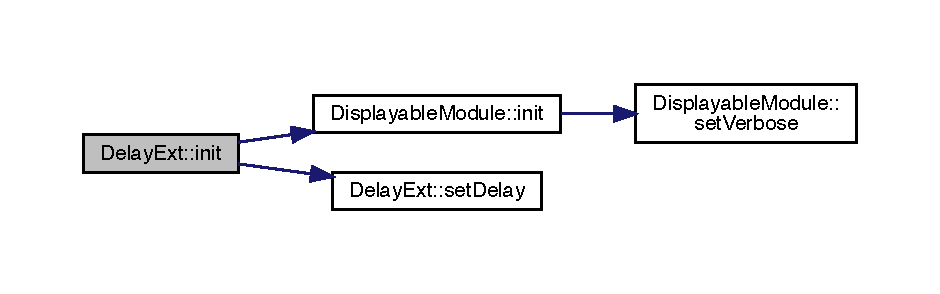
\includegraphics[width=350pt]{class_delay_ext_aa7e84d74c1080b5473a7401a5042b305_cgraph}
\end{center}
\end{figure}
\mbox{\Hypertarget{class_delay_ext_a76001b2a3aad7ce1a2e1220ab7387be4}\label{class_delay_ext_a76001b2a3aad7ce1a2e1220ab7387be4}} 
\index{Delay\+Ext@{Delay\+Ext}!notify@{notify}}
\index{notify@{notify}!Delay\+Ext@{Delay\+Ext}}
\subsubsection{\texorpdfstring{notify()}{notify()}}
{\footnotesize\ttfamily void Delay\+Ext\+::notify (\begin{DoxyParamCaption}\item[{int}]{channel,  }\item[{float}]{value }\end{DoxyParamCaption})\hspace{0.3cm}{\ttfamily [virtual]}}



Reimplemented from \mbox{\hyperlink{class_displayable_module_a8ae5383931f10c54cff2feef2bc07dee}{Displayable\+Module}}.

Here is the call graph for this function\+:\nopagebreak
\begin{figure}[H]
\begin{center}
\leavevmode
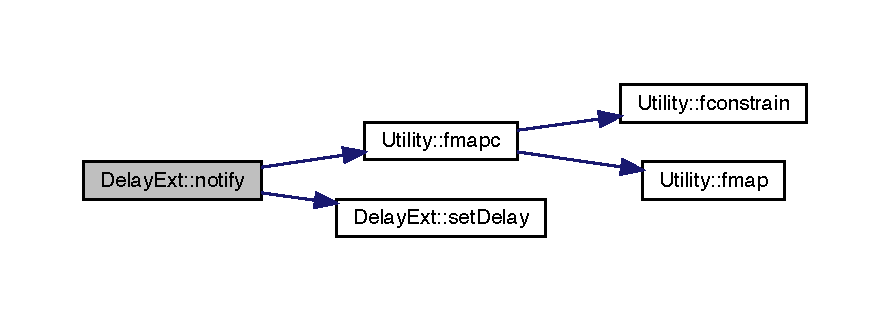
\includegraphics[width=350pt]{class_delay_ext_a76001b2a3aad7ce1a2e1220ab7387be4_cgraph}
\end{center}
\end{figure}
\mbox{\Hypertarget{class_delay_ext_a8b6e5eca2cdca8ea83a71cf57bec96dc}\label{class_delay_ext_a8b6e5eca2cdca8ea83a71cf57bec96dc}} 
\index{Delay\+Ext@{Delay\+Ext}!set\+Delay@{set\+Delay}}
\index{set\+Delay@{set\+Delay}!Delay\+Ext@{Delay\+Ext}}
\subsubsection{\texorpdfstring{set\+Delay()}{setDelay()}}
{\footnotesize\ttfamily void Delay\+Ext\+::set\+Delay (\begin{DoxyParamCaption}\item[{int}]{channel,  }\item[{int}]{delay\+\_\+ms }\end{DoxyParamCaption})}

Here is the caller graph for this function\+:\nopagebreak
\begin{figure}[H]
\begin{center}
\leavevmode
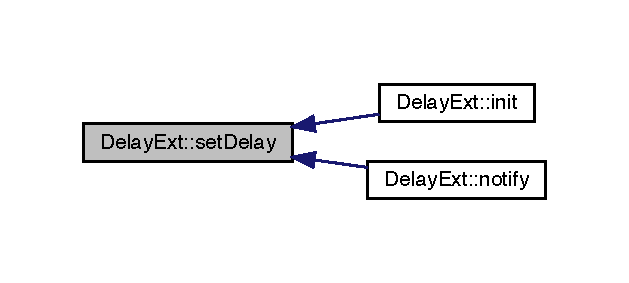
\includegraphics[width=302pt]{class_delay_ext_a8b6e5eca2cdca8ea83a71cf57bec96dc_icgraph}
\end{center}
\end{figure}
\mbox{\Hypertarget{class_delay_ext_aced3df43297e5f6092fc2a652ab712d2}\label{class_delay_ext_aced3df43297e5f6092fc2a652ab712d2}} 
\index{Delay\+Ext@{Delay\+Ext}!set\+Verbose@{set\+Verbose}}
\index{set\+Verbose@{set\+Verbose}!Delay\+Ext@{Delay\+Ext}}
\subsubsection{\texorpdfstring{set\+Verbose()}{setVerbose()}}
{\footnotesize\ttfamily void Delay\+Ext\+::set\+Verbose (\begin{DoxyParamCaption}\item[{int}]{verbose }\end{DoxyParamCaption})}



The documentation for this class was generated from the following files\+:\begin{DoxyCompactItemize}
\item 
\mbox{\hyperlink{_delay_ext_8h}{Delay\+Ext.\+h}}\item 
\mbox{\hyperlink{_delay_ext_8cpp}{Delay\+Ext.\+cpp}}\end{DoxyCompactItemize}

\hypertarget{class_displayable_module}{}\section{Displayable\+Module Class Reference}
\label{class_displayable_module}\index{Displayable\+Module@{Displayable\+Module}}


Base class for any class using the O\+L\+ED display.  




{\ttfamily \#include $<$Displayable\+Module.\+h$>$}



Inheritance diagram for Displayable\+Module\+:
\nopagebreak
\begin{figure}[H]
\begin{center}
\leavevmode
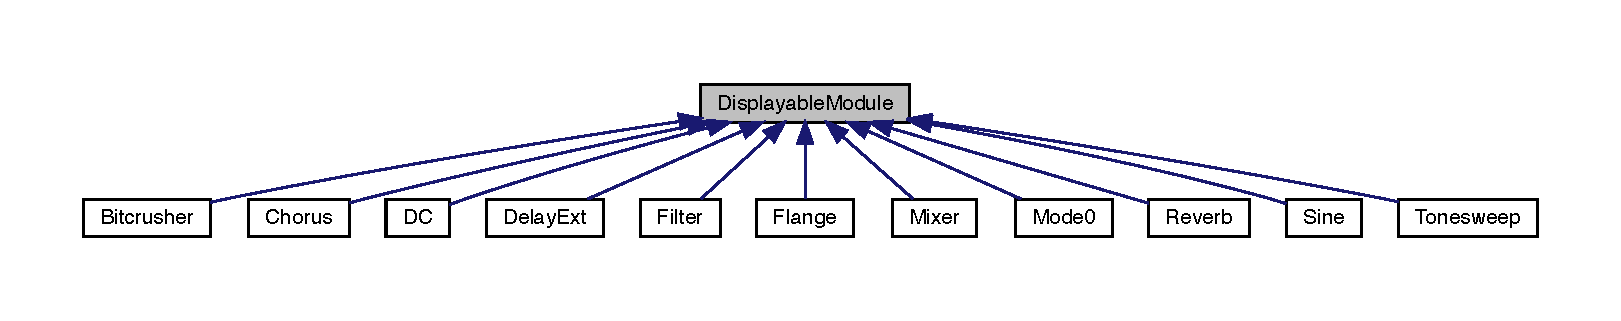
\includegraphics[width=350pt]{class_displayable_module__inherit__graph}
\end{center}
\end{figure}


Collaboration diagram for Displayable\+Module\+:
\nopagebreak
\begin{figure}[H]
\begin{center}
\leavevmode
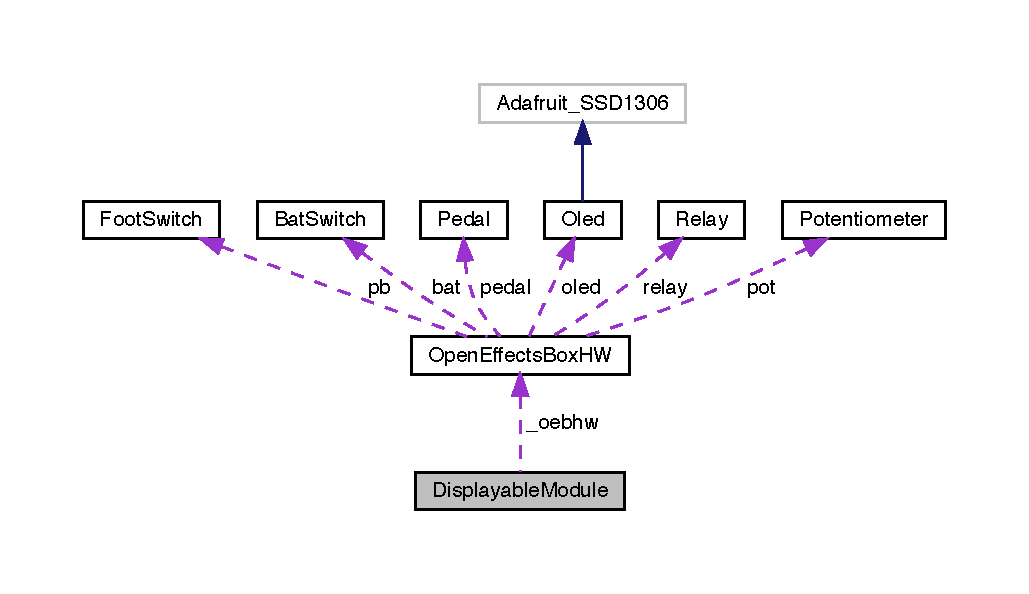
\includegraphics[width=350pt]{class_displayable_module__coll__graph}
\end{center}
\end{figure}
\subsection*{Public Member Functions}
\begin{DoxyCompactItemize}
\item 
\mbox{\hyperlink{class_displayable_module_a2495c334435664dba66160a00193ca7f}{Displayable\+Module}} ()
\item 
void \mbox{\hyperlink{class_displayable_module_a3c659ed0797811970d156ce342cdb187}{set\+Verbose}} (int verbose)
\item 
void \mbox{\hyperlink{class_displayable_module_a12010231a6a049a1110b642cc1c83efd}{init}} (int id, char $\ast$name, \mbox{\hyperlink{class_open_effects_box_h_w}{Open\+Effects\+Box\+HW}} $\ast$oebhw, int verbose=\mbox{\hyperlink{_displayable_module_8h_a483eb167fdc6365824170a77f4900236}{Displayable\+Module\+\_\+\+V\+E\+R\+B\+O\+S\+E\+\_\+\+D\+E\+F\+A\+U\+LT}})
\item 
bool \mbox{\hyperlink{class_displayable_module_ac681bcbdec3aa9daeb1d9ade59f0313c}{is\+Active}} ()
\item 
void \mbox{\hyperlink{class_displayable_module_a829fc6e70ddf9286a0772e3c1d173e7e}{activate}} (bool val)
\item 
virtual void \mbox{\hyperlink{class_displayable_module_a8ae5383931f10c54cff2feef2bc07dee}{notify}} (int channel, float value)
\item 
virtual void \mbox{\hyperlink{class_displayable_module_a02de26d62ef508cae9ed07920e21784d}{display}} (int mode, int sub\+Mode, bool force=false)
\end{DoxyCompactItemize}
\subsection*{Protected Attributes}
\begin{DoxyCompactItemize}
\item 
int \mbox{\hyperlink{class_displayable_module_a1688c41afaaae55f3c9597ee263904d0}{\+\_\+verbose}}
\item 
int \mbox{\hyperlink{class_displayable_module_af06d4fc8c566bb4bb23a46b4c9951826}{\+\_\+id}}
\item 
char \mbox{\hyperlink{class_displayable_module_af26ba38e9f363b6c427c53871ecd6a82}{\+\_\+name}} \mbox{[}\mbox{\hyperlink{_displayable_module_8h_a24a04c2abf64a124761ed400e373354f}{name\+Str\+Len}}\mbox{]}
\item 
\mbox{\hyperlink{class_open_effects_box_h_w}{Open\+Effects\+Box\+HW}} $\ast$ \mbox{\hyperlink{class_displayable_module_a9d2fcd94a6963583f8b4207fb0ee293f}{\+\_\+oebhw}}
\item 
bool \mbox{\hyperlink{class_displayable_module_a3f7442a98e7b99e753270202b2301310}{\+\_\+is\+Active}}
\item 
bool \mbox{\hyperlink{class_displayable_module_add6db9c66946829488facc41a8a9331a}{\+\_\+display\+Is\+Stale}}
\end{DoxyCompactItemize}


\subsection{Detailed Description}
Base class for any class using the O\+L\+ED display. 

In order to limit the delays involved in calling \mbox{\hyperlink{class_displayable_module_a02de26d62ef508cae9ed07920e21784d}{display()}} to the O\+L\+ED, we want to re-\/render the display only when something changes that is reflected on the current display. This base class provides the instance variables to keep track of that. 

\subsection{Constructor \& Destructor Documentation}
\mbox{\Hypertarget{class_displayable_module_a2495c334435664dba66160a00193ca7f}\label{class_displayable_module_a2495c334435664dba66160a00193ca7f}} 
\index{Displayable\+Module@{Displayable\+Module}!Displayable\+Module@{Displayable\+Module}}
\index{Displayable\+Module@{Displayable\+Module}!Displayable\+Module@{Displayable\+Module}}
\subsubsection{\texorpdfstring{Displayable\+Module()}{DisplayableModule()}}
{\footnotesize\ttfamily Displayable\+Module\+::\+Displayable\+Module (\begin{DoxyParamCaption}{ }\end{DoxyParamCaption})}



\subsection{Member Function Documentation}
\mbox{\Hypertarget{class_displayable_module_a829fc6e70ddf9286a0772e3c1d173e7e}\label{class_displayable_module_a829fc6e70ddf9286a0772e3c1d173e7e}} 
\index{Displayable\+Module@{Displayable\+Module}!activate@{activate}}
\index{activate@{activate}!Displayable\+Module@{Displayable\+Module}}
\subsubsection{\texorpdfstring{activate()}{activate()}}
{\footnotesize\ttfamily void Displayable\+Module\+::activate (\begin{DoxyParamCaption}\item[{bool}]{val }\end{DoxyParamCaption})}

\mbox{\Hypertarget{class_displayable_module_a02de26d62ef508cae9ed07920e21784d}\label{class_displayable_module_a02de26d62ef508cae9ed07920e21784d}} 
\index{Displayable\+Module@{Displayable\+Module}!display@{display}}
\index{display@{display}!Displayable\+Module@{Displayable\+Module}}
\subsubsection{\texorpdfstring{display()}{display()}}
{\footnotesize\ttfamily void Displayable\+Module\+::display (\begin{DoxyParamCaption}\item[{int}]{mode,  }\item[{int}]{sub\+Mode,  }\item[{bool}]{force = {\ttfamily false} }\end{DoxyParamCaption})\hspace{0.3cm}{\ttfamily [virtual]}}



Reimplemented in \mbox{\hyperlink{class_delay_ext_a53d22982c98ab7cc1206744304ecd5a9}{Delay\+Ext}}, \mbox{\hyperlink{class_filter_a3a2062c5c576d18cd734546ca41d29ad}{Filter}}, \mbox{\hyperlink{class_mixer_a13c7c7e025c83d2f9a22b4c16b400551}{Mixer}}, \mbox{\hyperlink{class_bitcrusher_aa5d365b3690a76f968465b9e841720f6}{Bitcrusher}}, \mbox{\hyperlink{class_mode0_a7d43e749cfd1831974f36d7d8e54e221}{Mode0}}, \mbox{\hyperlink{class_chorus_a6a28900025c58af59c7eb70f49347422}{Chorus}}, \mbox{\hyperlink{class_d_c_a006f266e63bdff5042fa2c443e1a04cc}{DC}}, \mbox{\hyperlink{class_reverb_aaf90c9b334f7e1c869c5b406ada68135}{Reverb}}, \mbox{\hyperlink{class_flange_afce68b7e8538cf7bfacdcec8d603f602}{Flange}}, \mbox{\hyperlink{class_sine_a1fcdbe7a2ac18201dfc30cb1dca0b3b3}{Sine}}, and \mbox{\hyperlink{class_tonesweep_ad16e1b0c7eb84827c3ee8a6ae43b0e81}{Tonesweep}}.

\mbox{\Hypertarget{class_displayable_module_a12010231a6a049a1110b642cc1c83efd}\label{class_displayable_module_a12010231a6a049a1110b642cc1c83efd}} 
\index{Displayable\+Module@{Displayable\+Module}!init@{init}}
\index{init@{init}!Displayable\+Module@{Displayable\+Module}}
\subsubsection{\texorpdfstring{init()}{init()}}
{\footnotesize\ttfamily void Displayable\+Module\+::init (\begin{DoxyParamCaption}\item[{int}]{id,  }\item[{char $\ast$}]{name,  }\item[{\mbox{\hyperlink{class_open_effects_box_h_w}{Open\+Effects\+Box\+HW}} $\ast$}]{oebhw,  }\item[{int}]{verbose = {\ttfamily \mbox{\hyperlink{_displayable_module_8h_a483eb167fdc6365824170a77f4900236}{Displayable\+Module\+\_\+\+V\+E\+R\+B\+O\+S\+E\+\_\+\+D\+E\+F\+A\+U\+LT}}} }\end{DoxyParamCaption})}

Here is the call graph for this function\+:\nopagebreak
\begin{figure}[H]
\begin{center}
\leavevmode
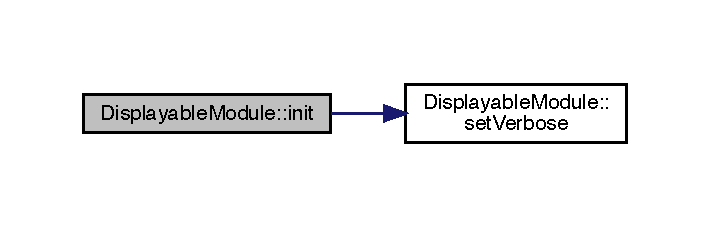
\includegraphics[width=341pt]{class_displayable_module_a12010231a6a049a1110b642cc1c83efd_cgraph}
\end{center}
\end{figure}
Here is the caller graph for this function\+:\nopagebreak
\begin{figure}[H]
\begin{center}
\leavevmode
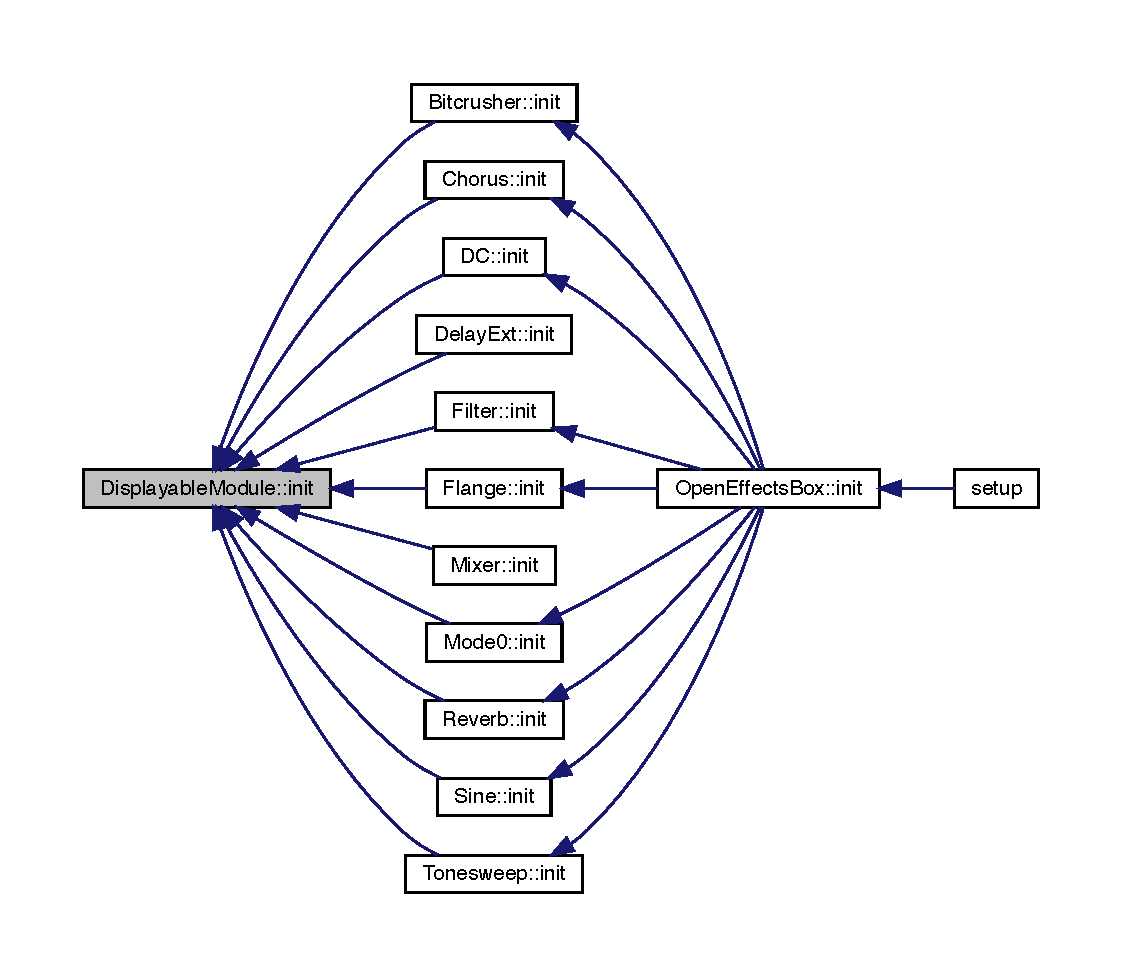
\includegraphics[width=350pt]{class_displayable_module_a12010231a6a049a1110b642cc1c83efd_icgraph}
\end{center}
\end{figure}
\mbox{\Hypertarget{class_displayable_module_ac681bcbdec3aa9daeb1d9ade59f0313c}\label{class_displayable_module_ac681bcbdec3aa9daeb1d9ade59f0313c}} 
\index{Displayable\+Module@{Displayable\+Module}!is\+Active@{is\+Active}}
\index{is\+Active@{is\+Active}!Displayable\+Module@{Displayable\+Module}}
\subsubsection{\texorpdfstring{is\+Active()}{isActive()}}
{\footnotesize\ttfamily bool Displayable\+Module\+::is\+Active (\begin{DoxyParamCaption}{ }\end{DoxyParamCaption})}

\mbox{\Hypertarget{class_displayable_module_a8ae5383931f10c54cff2feef2bc07dee}\label{class_displayable_module_a8ae5383931f10c54cff2feef2bc07dee}} 
\index{Displayable\+Module@{Displayable\+Module}!notify@{notify}}
\index{notify@{notify}!Displayable\+Module@{Displayable\+Module}}
\subsubsection{\texorpdfstring{notify()}{notify()}}
{\footnotesize\ttfamily void Displayable\+Module\+::notify (\begin{DoxyParamCaption}\item[{int}]{channel,  }\item[{float}]{value }\end{DoxyParamCaption})\hspace{0.3cm}{\ttfamily [virtual]}}



Reimplemented in \mbox{\hyperlink{class_delay_ext_a76001b2a3aad7ce1a2e1220ab7387be4}{Delay\+Ext}}, \mbox{\hyperlink{class_filter_a9cdce58ac2fe0b8beb6d561ab3725041}{Filter}}, \mbox{\hyperlink{class_mixer_a73177ee1e071909ef23ff2e913eb6cbc}{Mixer}}, \mbox{\hyperlink{class_bitcrusher_ae392ad4b140a5121df417ece060911f4}{Bitcrusher}}, \mbox{\hyperlink{class_mode0_a743ebe3d0faccc421d06c9114026a099}{Mode0}}, \mbox{\hyperlink{class_chorus_acb22e9cc93011859d1ae02b05a7388f5}{Chorus}}, \mbox{\hyperlink{class_d_c_a45e51132fbd69668134f3ab13f3668b1}{DC}}, \mbox{\hyperlink{class_reverb_a0a4818faef8203311b3c31eb9d59c277}{Reverb}}, \mbox{\hyperlink{class_flange_a10541758c108d92a73e96ed9f8f1377b}{Flange}}, \mbox{\hyperlink{class_sine_a91e8327318758647ea3e0f856eb3eb60}{Sine}}, and \mbox{\hyperlink{class_tonesweep_a26d324fb0de4aac00a04e7e7e9e812c0}{Tonesweep}}.

\mbox{\Hypertarget{class_displayable_module_a3c659ed0797811970d156ce342cdb187}\label{class_displayable_module_a3c659ed0797811970d156ce342cdb187}} 
\index{Displayable\+Module@{Displayable\+Module}!set\+Verbose@{set\+Verbose}}
\index{set\+Verbose@{set\+Verbose}!Displayable\+Module@{Displayable\+Module}}
\subsubsection{\texorpdfstring{set\+Verbose()}{setVerbose()}}
{\footnotesize\ttfamily void Displayable\+Module\+::set\+Verbose (\begin{DoxyParamCaption}\item[{int}]{verbose }\end{DoxyParamCaption})}

Here is the caller graph for this function\+:\nopagebreak
\begin{figure}[H]
\begin{center}
\leavevmode
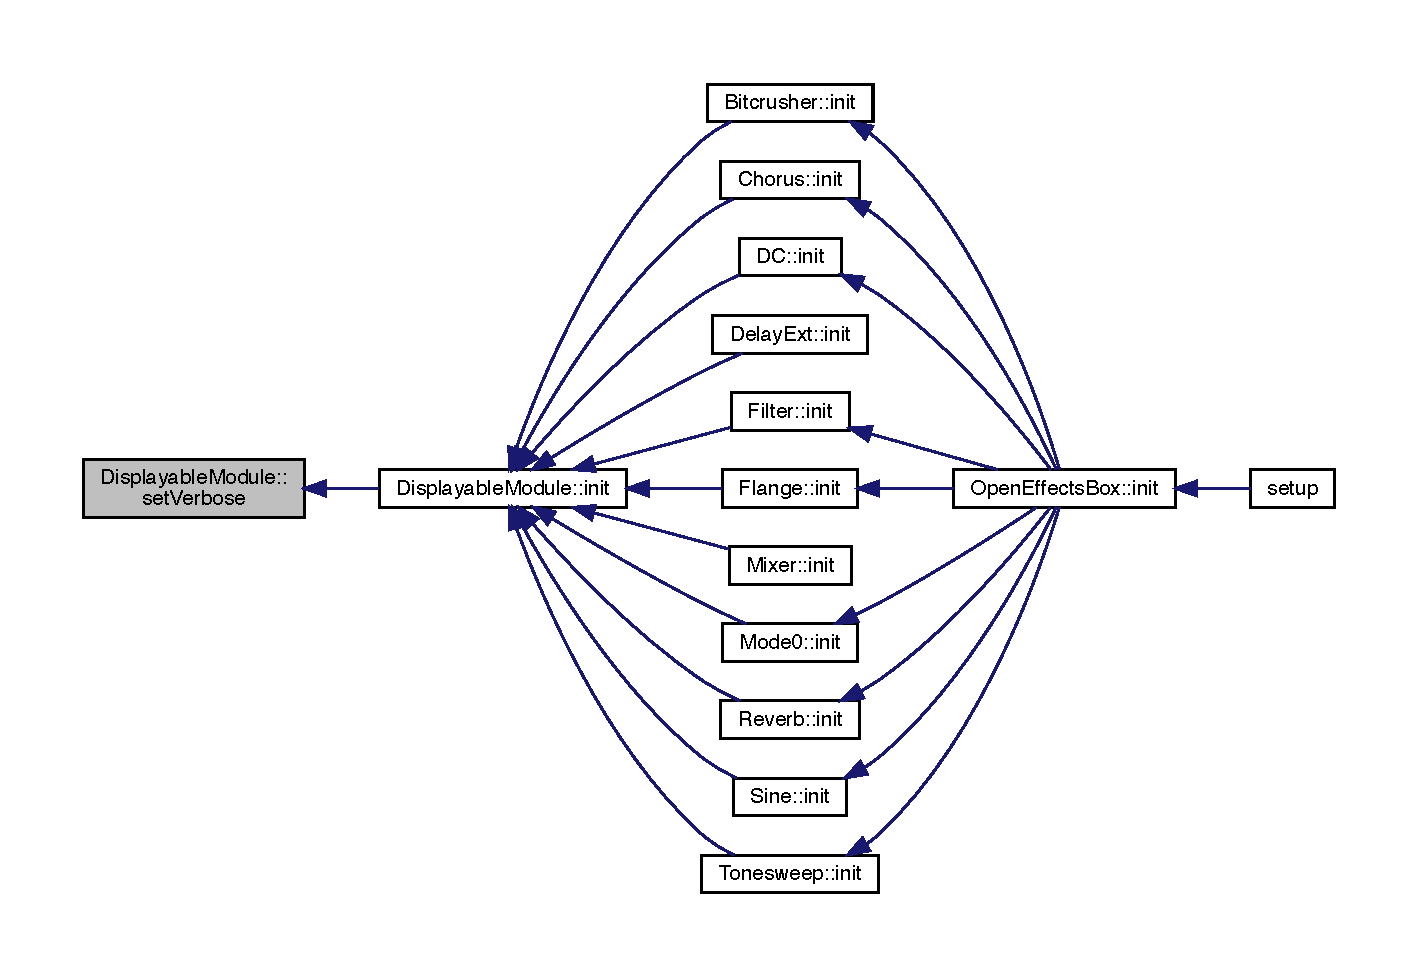
\includegraphics[width=350pt]{class_displayable_module_a3c659ed0797811970d156ce342cdb187_icgraph}
\end{center}
\end{figure}


\subsection{Member Data Documentation}
\mbox{\Hypertarget{class_displayable_module_add6db9c66946829488facc41a8a9331a}\label{class_displayable_module_add6db9c66946829488facc41a8a9331a}} 
\index{Displayable\+Module@{Displayable\+Module}!\+\_\+display\+Is\+Stale@{\+\_\+display\+Is\+Stale}}
\index{\+\_\+display\+Is\+Stale@{\+\_\+display\+Is\+Stale}!Displayable\+Module@{Displayable\+Module}}
\subsubsection{\texorpdfstring{\+\_\+display\+Is\+Stale}{\_displayIsStale}}
{\footnotesize\ttfamily bool Displayable\+Module\+::\+\_\+display\+Is\+Stale\hspace{0.3cm}{\ttfamily [protected]}}

\mbox{\Hypertarget{class_displayable_module_af06d4fc8c566bb4bb23a46b4c9951826}\label{class_displayable_module_af06d4fc8c566bb4bb23a46b4c9951826}} 
\index{Displayable\+Module@{Displayable\+Module}!\+\_\+id@{\+\_\+id}}
\index{\+\_\+id@{\+\_\+id}!Displayable\+Module@{Displayable\+Module}}
\subsubsection{\texorpdfstring{\+\_\+id}{\_id}}
{\footnotesize\ttfamily int Displayable\+Module\+::\+\_\+id\hspace{0.3cm}{\ttfamily [protected]}}

\mbox{\Hypertarget{class_displayable_module_a3f7442a98e7b99e753270202b2301310}\label{class_displayable_module_a3f7442a98e7b99e753270202b2301310}} 
\index{Displayable\+Module@{Displayable\+Module}!\+\_\+is\+Active@{\+\_\+is\+Active}}
\index{\+\_\+is\+Active@{\+\_\+is\+Active}!Displayable\+Module@{Displayable\+Module}}
\subsubsection{\texorpdfstring{\+\_\+is\+Active}{\_isActive}}
{\footnotesize\ttfamily bool Displayable\+Module\+::\+\_\+is\+Active\hspace{0.3cm}{\ttfamily [protected]}}

\mbox{\Hypertarget{class_displayable_module_af26ba38e9f363b6c427c53871ecd6a82}\label{class_displayable_module_af26ba38e9f363b6c427c53871ecd6a82}} 
\index{Displayable\+Module@{Displayable\+Module}!\+\_\+name@{\+\_\+name}}
\index{\+\_\+name@{\+\_\+name}!Displayable\+Module@{Displayable\+Module}}
\subsubsection{\texorpdfstring{\+\_\+name}{\_name}}
{\footnotesize\ttfamily char Displayable\+Module\+::\+\_\+name\mbox{[}\mbox{\hyperlink{_displayable_module_8h_a24a04c2abf64a124761ed400e373354f}{name\+Str\+Len}}\mbox{]}\hspace{0.3cm}{\ttfamily [protected]}}

\mbox{\Hypertarget{class_displayable_module_a9d2fcd94a6963583f8b4207fb0ee293f}\label{class_displayable_module_a9d2fcd94a6963583f8b4207fb0ee293f}} 
\index{Displayable\+Module@{Displayable\+Module}!\+\_\+oebhw@{\+\_\+oebhw}}
\index{\+\_\+oebhw@{\+\_\+oebhw}!Displayable\+Module@{Displayable\+Module}}
\subsubsection{\texorpdfstring{\+\_\+oebhw}{\_oebhw}}
{\footnotesize\ttfamily \mbox{\hyperlink{class_open_effects_box_h_w}{Open\+Effects\+Box\+HW}}$\ast$ Displayable\+Module\+::\+\_\+oebhw\hspace{0.3cm}{\ttfamily [protected]}}

\mbox{\Hypertarget{class_displayable_module_a1688c41afaaae55f3c9597ee263904d0}\label{class_displayable_module_a1688c41afaaae55f3c9597ee263904d0}} 
\index{Displayable\+Module@{Displayable\+Module}!\+\_\+verbose@{\+\_\+verbose}}
\index{\+\_\+verbose@{\+\_\+verbose}!Displayable\+Module@{Displayable\+Module}}
\subsubsection{\texorpdfstring{\+\_\+verbose}{\_verbose}}
{\footnotesize\ttfamily int Displayable\+Module\+::\+\_\+verbose\hspace{0.3cm}{\ttfamily [protected]}}



The documentation for this class was generated from the following files\+:\begin{DoxyCompactItemize}
\item 
\mbox{\hyperlink{_displayable_module_8h}{Displayable\+Module.\+h}}\item 
\mbox{\hyperlink{_displayable_module_8cpp}{Displayable\+Module.\+cpp}}\end{DoxyCompactItemize}

\hypertarget{class_filter}{}\section{Filter Class Reference}
\label{class_filter}\index{Filter@{Filter}}


Wrapper for Audio Design Tool -\/\+Filter-\/.  




{\ttfamily \#include $<$Filter.\+h$>$}



Inheritance diagram for Filter\+:
\nopagebreak
\begin{figure}[H]
\begin{center}
\leavevmode
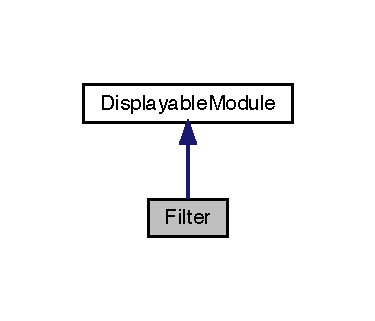
\includegraphics[width=180pt]{class_filter__inherit__graph}
\end{center}
\end{figure}


Collaboration diagram for Filter\+:
\nopagebreak
\begin{figure}[H]
\begin{center}
\leavevmode
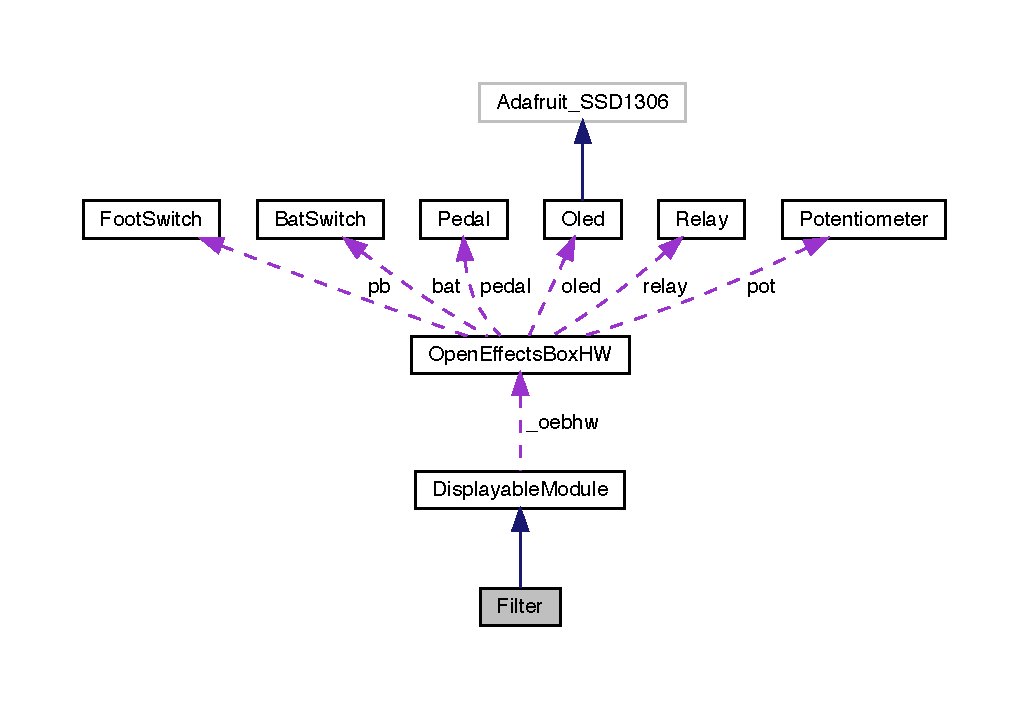
\includegraphics[width=350pt]{class_filter__coll__graph}
\end{center}
\end{figure}
\subsection*{Public Member Functions}
\begin{DoxyCompactItemize}
\item 
\mbox{\hyperlink{class_filter_ad15994c30d497afd567a6445446a249e}{Filter}} ()
\item 
void \mbox{\hyperlink{class_filter_aff18613de2ab3bc90035babc58c7b055}{set\+Verbose}} (int verbose)
\item 
void \mbox{\hyperlink{class_filter_acff0d2a488a223caa11d48a6147c7feb}{init}} (int id, char $\ast$name, Audio\+Filter\+State\+Variable $\ast$filter, \mbox{\hyperlink{class_open_effects_box_h_w}{Open\+Effects\+Box\+HW}} $\ast$oebhw, int verbose=\mbox{\hyperlink{_filter_8h_aeedb664ae18205202837764d021883e7}{Filter\+\_\+\+V\+E\+R\+B\+O\+S\+E\+\_\+\+D\+E\+F\+A\+U\+LT}})
\item 
void \mbox{\hyperlink{class_filter_a9cdce58ac2fe0b8beb6d561ab3725041}{notify}} (int channel, float value)
\item 
void \mbox{\hyperlink{class_filter_a3a2062c5c576d18cd734546ca41d29ad}{display}} (int mode, int sub\+Mode, bool force=false)
\item 
void \mbox{\hyperlink{class_filter_afe0720f8c3ed40208ebe59d894bf0645}{set\+Frequency}} (float frequency)
\item 
void \mbox{\hyperlink{class_filter_a9bd50f058259b8c3bc83daf99cdc9837}{set\+Resonance}} (float resonance)
\item 
void \mbox{\hyperlink{class_filter_ad4e47469cb53f7c7e3f95021c30599cc}{set\+Octave\+Control}} (float octave\+Control)
\end{DoxyCompactItemize}
\subsection*{Additional Inherited Members}


\subsection{Detailed Description}
Wrapper for Audio Design Tool -\/\+Filter-\/. 

See \href{https://www.pjrc.com/teensy/gui/}{\tt Paul Stoffregen\textquotesingle{}s Audio Design Tool}

Also see the Wikipedia article on \href{https://en.wikipedia.org/wiki/Wah-wah_pedal}{\tt Wah-\/wah pedals} I am trying to create a wah-\/wah pedal using an expression pedal routed to control the base frequency of this filter. 

\subsection{Constructor \& Destructor Documentation}
\mbox{\Hypertarget{class_filter_ad15994c30d497afd567a6445446a249e}\label{class_filter_ad15994c30d497afd567a6445446a249e}} 
\index{Filter@{Filter}!Filter@{Filter}}
\index{Filter@{Filter}!Filter@{Filter}}
\subsubsection{\texorpdfstring{Filter()}{Filter()}}
{\footnotesize\ttfamily Filter\+::\+Filter (\begin{DoxyParamCaption}{ }\end{DoxyParamCaption})}



\subsection{Member Function Documentation}
\mbox{\Hypertarget{class_filter_a3a2062c5c576d18cd734546ca41d29ad}\label{class_filter_a3a2062c5c576d18cd734546ca41d29ad}} 
\index{Filter@{Filter}!display@{display}}
\index{display@{display}!Filter@{Filter}}
\subsubsection{\texorpdfstring{display()}{display()}}
{\footnotesize\ttfamily void Filter\+::display (\begin{DoxyParamCaption}\item[{int}]{mode,  }\item[{int}]{sub\+Mode,  }\item[{bool}]{force = {\ttfamily false} }\end{DoxyParamCaption})\hspace{0.3cm}{\ttfamily [virtual]}}



Reimplemented from \mbox{\hyperlink{class_displayable_module_a02de26d62ef508cae9ed07920e21784d}{Displayable\+Module}}.

Here is the call graph for this function\+:\nopagebreak
\begin{figure}[H]
\begin{center}
\leavevmode
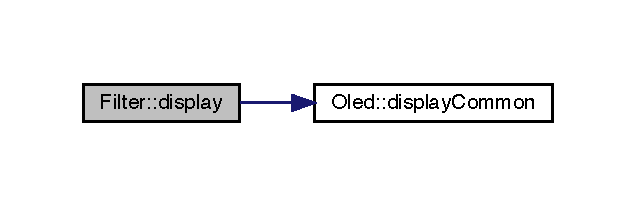
\includegraphics[width=305pt]{class_filter_a3a2062c5c576d18cd734546ca41d29ad_cgraph}
\end{center}
\end{figure}
\mbox{\Hypertarget{class_filter_acff0d2a488a223caa11d48a6147c7feb}\label{class_filter_acff0d2a488a223caa11d48a6147c7feb}} 
\index{Filter@{Filter}!init@{init}}
\index{init@{init}!Filter@{Filter}}
\subsubsection{\texorpdfstring{init()}{init()}}
{\footnotesize\ttfamily void Filter\+::init (\begin{DoxyParamCaption}\item[{int}]{id,  }\item[{char $\ast$}]{name,  }\item[{Audio\+Filter\+State\+Variable $\ast$}]{filter,  }\item[{\mbox{\hyperlink{class_open_effects_box_h_w}{Open\+Effects\+Box\+HW}} $\ast$}]{oebhw,  }\item[{int}]{verbose = {\ttfamily \mbox{\hyperlink{_filter_8h_aeedb664ae18205202837764d021883e7}{Filter\+\_\+\+V\+E\+R\+B\+O\+S\+E\+\_\+\+D\+E\+F\+A\+U\+LT}}} }\end{DoxyParamCaption})}

Here is the call graph for this function\+:\nopagebreak
\begin{figure}[H]
\begin{center}
\leavevmode
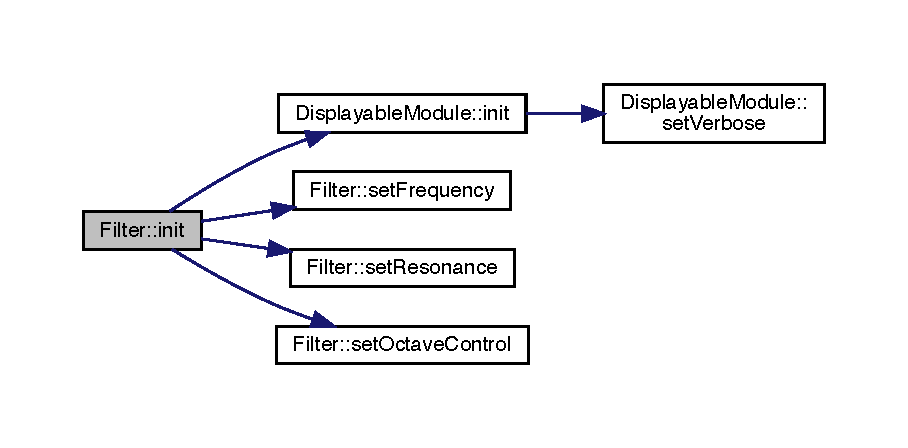
\includegraphics[width=350pt]{class_filter_acff0d2a488a223caa11d48a6147c7feb_cgraph}
\end{center}
\end{figure}
Here is the caller graph for this function\+:\nopagebreak
\begin{figure}[H]
\begin{center}
\leavevmode
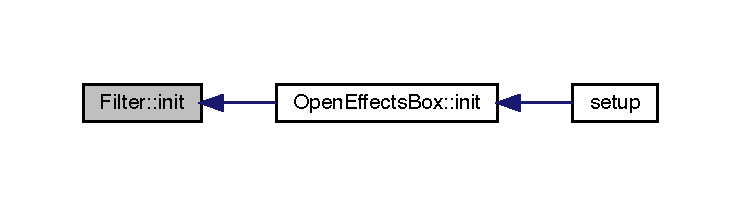
\includegraphics[width=350pt]{class_filter_acff0d2a488a223caa11d48a6147c7feb_icgraph}
\end{center}
\end{figure}
\mbox{\Hypertarget{class_filter_a9cdce58ac2fe0b8beb6d561ab3725041}\label{class_filter_a9cdce58ac2fe0b8beb6d561ab3725041}} 
\index{Filter@{Filter}!notify@{notify}}
\index{notify@{notify}!Filter@{Filter}}
\subsubsection{\texorpdfstring{notify()}{notify()}}
{\footnotesize\ttfamily void Filter\+::notify (\begin{DoxyParamCaption}\item[{int}]{channel,  }\item[{float}]{value }\end{DoxyParamCaption})\hspace{0.3cm}{\ttfamily [virtual]}}



Reimplemented from \mbox{\hyperlink{class_displayable_module_a8ae5383931f10c54cff2feef2bc07dee}{Displayable\+Module}}.

Here is the call graph for this function\+:\nopagebreak
\begin{figure}[H]
\begin{center}
\leavevmode
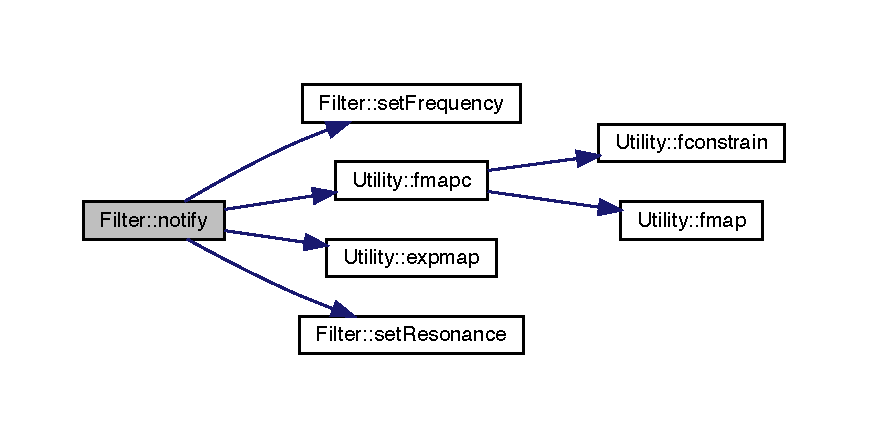
\includegraphics[width=350pt]{class_filter_a9cdce58ac2fe0b8beb6d561ab3725041_cgraph}
\end{center}
\end{figure}
\mbox{\Hypertarget{class_filter_afe0720f8c3ed40208ebe59d894bf0645}\label{class_filter_afe0720f8c3ed40208ebe59d894bf0645}} 
\index{Filter@{Filter}!set\+Frequency@{set\+Frequency}}
\index{set\+Frequency@{set\+Frequency}!Filter@{Filter}}
\subsubsection{\texorpdfstring{set\+Frequency()}{setFrequency()}}
{\footnotesize\ttfamily void Filter\+::set\+Frequency (\begin{DoxyParamCaption}\item[{float}]{frequency }\end{DoxyParamCaption})}

Here is the caller graph for this function\+:\nopagebreak
\begin{figure}[H]
\begin{center}
\leavevmode
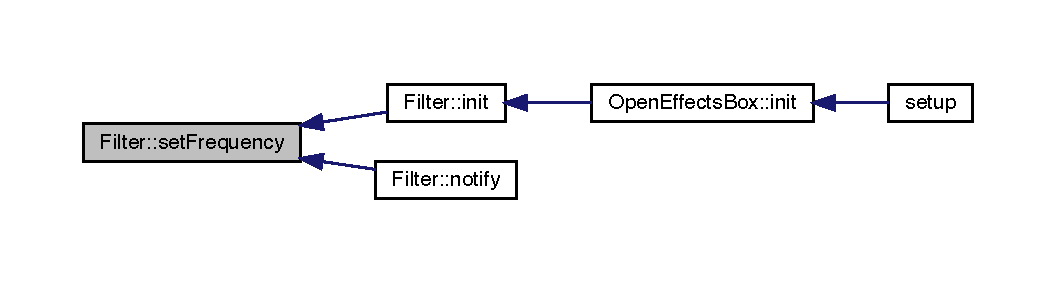
\includegraphics[width=350pt]{class_filter_afe0720f8c3ed40208ebe59d894bf0645_icgraph}
\end{center}
\end{figure}
\mbox{\Hypertarget{class_filter_ad4e47469cb53f7c7e3f95021c30599cc}\label{class_filter_ad4e47469cb53f7c7e3f95021c30599cc}} 
\index{Filter@{Filter}!set\+Octave\+Control@{set\+Octave\+Control}}
\index{set\+Octave\+Control@{set\+Octave\+Control}!Filter@{Filter}}
\subsubsection{\texorpdfstring{set\+Octave\+Control()}{setOctaveControl()}}
{\footnotesize\ttfamily void Filter\+::set\+Octave\+Control (\begin{DoxyParamCaption}\item[{float}]{octave\+Control }\end{DoxyParamCaption})}

Here is the caller graph for this function\+:\nopagebreak
\begin{figure}[H]
\begin{center}
\leavevmode
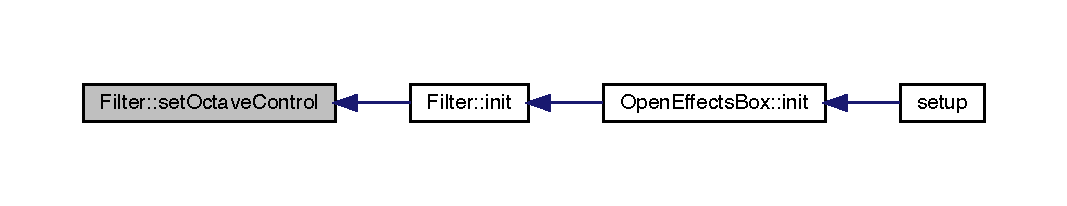
\includegraphics[width=350pt]{class_filter_ad4e47469cb53f7c7e3f95021c30599cc_icgraph}
\end{center}
\end{figure}
\mbox{\Hypertarget{class_filter_a9bd50f058259b8c3bc83daf99cdc9837}\label{class_filter_a9bd50f058259b8c3bc83daf99cdc9837}} 
\index{Filter@{Filter}!set\+Resonance@{set\+Resonance}}
\index{set\+Resonance@{set\+Resonance}!Filter@{Filter}}
\subsubsection{\texorpdfstring{set\+Resonance()}{setResonance()}}
{\footnotesize\ttfamily void Filter\+::set\+Resonance (\begin{DoxyParamCaption}\item[{float}]{resonance }\end{DoxyParamCaption})}

Here is the caller graph for this function\+:\nopagebreak
\begin{figure}[H]
\begin{center}
\leavevmode
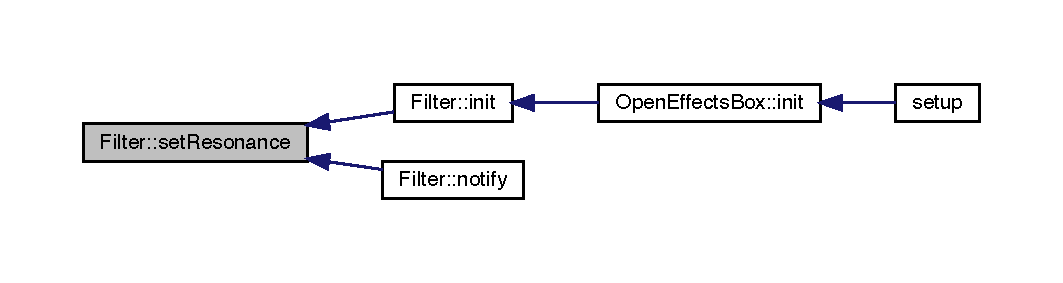
\includegraphics[width=350pt]{class_filter_a9bd50f058259b8c3bc83daf99cdc9837_icgraph}
\end{center}
\end{figure}
\mbox{\Hypertarget{class_filter_aff18613de2ab3bc90035babc58c7b055}\label{class_filter_aff18613de2ab3bc90035babc58c7b055}} 
\index{Filter@{Filter}!set\+Verbose@{set\+Verbose}}
\index{set\+Verbose@{set\+Verbose}!Filter@{Filter}}
\subsubsection{\texorpdfstring{set\+Verbose()}{setVerbose()}}
{\footnotesize\ttfamily void Filter\+::set\+Verbose (\begin{DoxyParamCaption}\item[{int}]{verbose }\end{DoxyParamCaption})}



The documentation for this class was generated from the following files\+:\begin{DoxyCompactItemize}
\item 
\mbox{\hyperlink{_filter_8h}{Filter.\+h}}\item 
\mbox{\hyperlink{_filter_8cpp}{Filter.\+cpp}}\end{DoxyCompactItemize}

\hypertarget{class_flange}{}\section{Flange Class Reference}
\label{class_flange}\index{Flange@{Flange}}


Wrapper for Audio Design Tool -\/\+Flange-\/.  




{\ttfamily \#include $<$Flange.\+h$>$}



Inheritance diagram for Flange\+:
\nopagebreak
\begin{figure}[H]
\begin{center}
\leavevmode
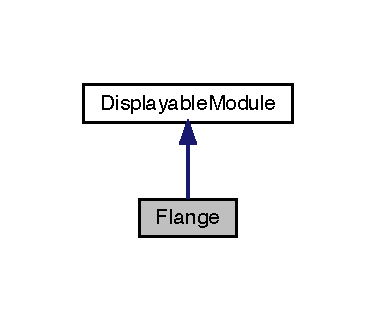
\includegraphics[width=180pt]{class_flange__inherit__graph}
\end{center}
\end{figure}


Collaboration diagram for Flange\+:
\nopagebreak
\begin{figure}[H]
\begin{center}
\leavevmode
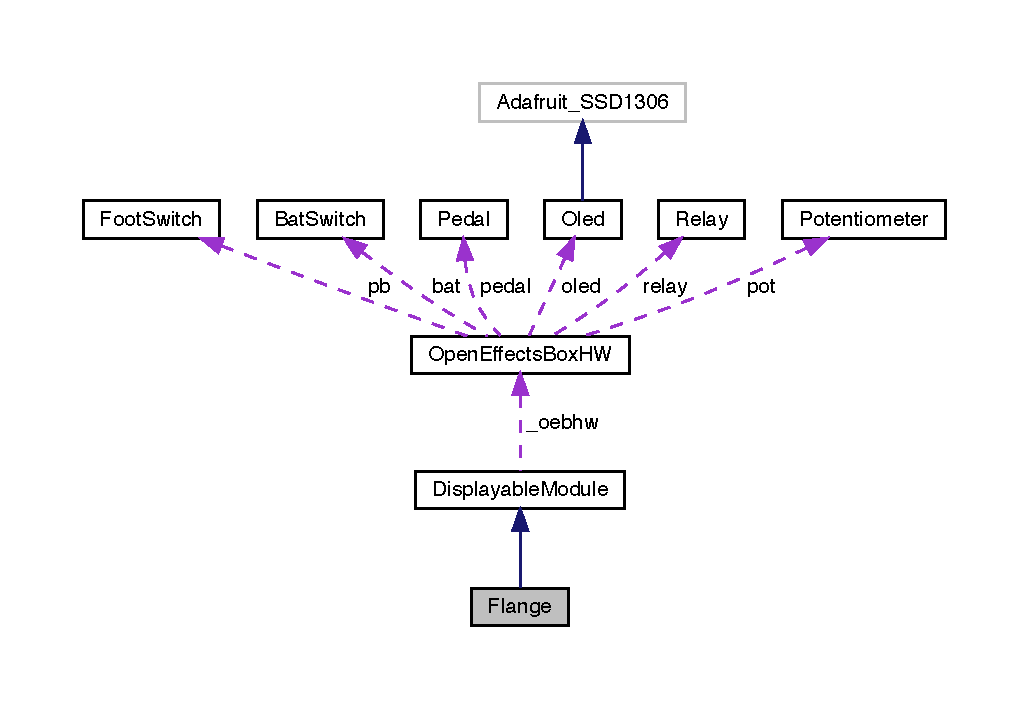
\includegraphics[width=350pt]{class_flange__coll__graph}
\end{center}
\end{figure}
\subsection*{Public Member Functions}
\begin{DoxyCompactItemize}
\item 
\mbox{\hyperlink{class_flange_ab4ec2beb299cf097f76d090545f6e34f}{Flange}} ()
\item 
void \mbox{\hyperlink{class_flange_ac44903a68dbb8a6de019b3f1e7205461}{set\+Verbose}} (int verbose)
\item 
void \mbox{\hyperlink{class_flange_a0b08351febfa39989acb6446c096346e}{init}} (int id, char $\ast$name, Audio\+Effect\+Flange $\ast$flange, \mbox{\hyperlink{class_open_effects_box_h_w}{Open\+Effects\+Box\+HW}} $\ast$oebhw, int verbose=\mbox{\hyperlink{_flange_8h_abe629c5baa4633f9806318a67d486437}{Flange\+\_\+\+V\+E\+R\+B\+O\+S\+E\+\_\+\+D\+E\+F\+A\+U\+LT}})
\item 
void \mbox{\hyperlink{class_flange_a10541758c108d92a73e96ed9f8f1377b}{notify}} (int channel, float value)
\item 
void \mbox{\hyperlink{class_flange_afce68b7e8538cf7bfacdcec8d603f602}{display}} (int mode, int sub\+Mode, bool force=false)
\item 
void \mbox{\hyperlink{class_flange_a733bc8118f327fc4c31c896642ad49ad}{set\+Offset}} (int offset)
\item 
void \mbox{\hyperlink{class_flange_a34ba641893065a297d5fe767a1fa2fc4}{set\+Depth}} (int depth)
\item 
void \mbox{\hyperlink{class_flange_af132f265ce1567691ffa2ce29bb512c6}{set\+Delay\+Freq}} (float delay\+Freq)
\end{DoxyCompactItemize}
\subsection*{Additional Inherited Members}


\subsection{Detailed Description}
Wrapper for Audio Design Tool -\/\+Flange-\/. 

See \href{https://www.pjrc.com/teensy/gui/}{\tt Paul Stoffregen\textquotesingle{}s Audio Design Tool} 

\subsection{Constructor \& Destructor Documentation}
\mbox{\Hypertarget{class_flange_ab4ec2beb299cf097f76d090545f6e34f}\label{class_flange_ab4ec2beb299cf097f76d090545f6e34f}} 
\index{Flange@{Flange}!Flange@{Flange}}
\index{Flange@{Flange}!Flange@{Flange}}
\subsubsection{\texorpdfstring{Flange()}{Flange()}}
{\footnotesize\ttfamily Flange\+::\+Flange (\begin{DoxyParamCaption}{ }\end{DoxyParamCaption})}



\subsection{Member Function Documentation}
\mbox{\Hypertarget{class_flange_afce68b7e8538cf7bfacdcec8d603f602}\label{class_flange_afce68b7e8538cf7bfacdcec8d603f602}} 
\index{Flange@{Flange}!display@{display}}
\index{display@{display}!Flange@{Flange}}
\subsubsection{\texorpdfstring{display()}{display()}}
{\footnotesize\ttfamily void Flange\+::display (\begin{DoxyParamCaption}\item[{int}]{mode,  }\item[{int}]{sub\+Mode,  }\item[{bool}]{force = {\ttfamily false} }\end{DoxyParamCaption})\hspace{0.3cm}{\ttfamily [virtual]}}



Reimplemented from \mbox{\hyperlink{class_displayable_module_a02de26d62ef508cae9ed07920e21784d}{Displayable\+Module}}.

Here is the call graph for this function\+:\nopagebreak
\begin{figure}[H]
\begin{center}
\leavevmode
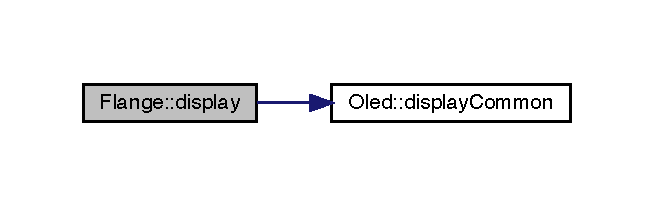
\includegraphics[width=314pt]{class_flange_afce68b7e8538cf7bfacdcec8d603f602_cgraph}
\end{center}
\end{figure}
\mbox{\Hypertarget{class_flange_a0b08351febfa39989acb6446c096346e}\label{class_flange_a0b08351febfa39989acb6446c096346e}} 
\index{Flange@{Flange}!init@{init}}
\index{init@{init}!Flange@{Flange}}
\subsubsection{\texorpdfstring{init()}{init()}}
{\footnotesize\ttfamily void Flange\+::init (\begin{DoxyParamCaption}\item[{int}]{id,  }\item[{char $\ast$}]{name,  }\item[{Audio\+Effect\+Flange $\ast$}]{flange,  }\item[{\mbox{\hyperlink{class_open_effects_box_h_w}{Open\+Effects\+Box\+HW}} $\ast$}]{oebhw,  }\item[{int}]{verbose = {\ttfamily \mbox{\hyperlink{_flange_8h_abe629c5baa4633f9806318a67d486437}{Flange\+\_\+\+V\+E\+R\+B\+O\+S\+E\+\_\+\+D\+E\+F\+A\+U\+LT}}} }\end{DoxyParamCaption})}

Here is the call graph for this function\+:\nopagebreak
\begin{figure}[H]
\begin{center}
\leavevmode
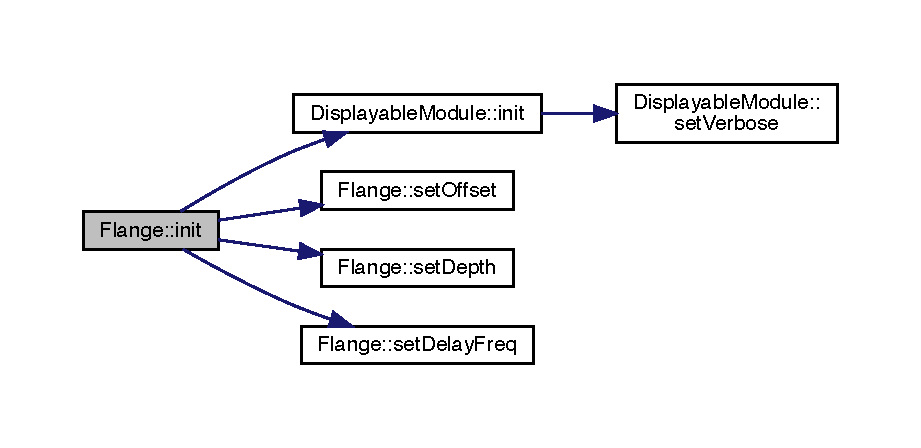
\includegraphics[width=350pt]{class_flange_a0b08351febfa39989acb6446c096346e_cgraph}
\end{center}
\end{figure}
Here is the caller graph for this function\+:\nopagebreak
\begin{figure}[H]
\begin{center}
\leavevmode
\includegraphics[width=350pt]{class_flange_a0b08351febfa39989acb6446c096346e_icgraph}
\end{center}
\end{figure}
\mbox{\Hypertarget{class_flange_a10541758c108d92a73e96ed9f8f1377b}\label{class_flange_a10541758c108d92a73e96ed9f8f1377b}} 
\index{Flange@{Flange}!notify@{notify}}
\index{notify@{notify}!Flange@{Flange}}
\subsubsection{\texorpdfstring{notify()}{notify()}}
{\footnotesize\ttfamily void Flange\+::notify (\begin{DoxyParamCaption}\item[{int}]{channel,  }\item[{float}]{value }\end{DoxyParamCaption})\hspace{0.3cm}{\ttfamily [virtual]}}



Reimplemented from \mbox{\hyperlink{class_displayable_module_a8ae5383931f10c54cff2feef2bc07dee}{Displayable\+Module}}.

Here is the call graph for this function\+:\nopagebreak
\begin{figure}[H]
\begin{center}
\leavevmode
\includegraphics[width=350pt]{class_flange_a10541758c108d92a73e96ed9f8f1377b_cgraph}
\end{center}
\end{figure}
\mbox{\Hypertarget{class_flange_af132f265ce1567691ffa2ce29bb512c6}\label{class_flange_af132f265ce1567691ffa2ce29bb512c6}} 
\index{Flange@{Flange}!set\+Delay\+Freq@{set\+Delay\+Freq}}
\index{set\+Delay\+Freq@{set\+Delay\+Freq}!Flange@{Flange}}
\subsubsection{\texorpdfstring{set\+Delay\+Freq()}{setDelayFreq()}}
{\footnotesize\ttfamily void Flange\+::set\+Delay\+Freq (\begin{DoxyParamCaption}\item[{float}]{delay\+Freq }\end{DoxyParamCaption})}

Here is the caller graph for this function\+:\nopagebreak
\begin{figure}[H]
\begin{center}
\leavevmode
\includegraphics[width=350pt]{class_flange_af132f265ce1567691ffa2ce29bb512c6_icgraph}
\end{center}
\end{figure}
\mbox{\Hypertarget{class_flange_a34ba641893065a297d5fe767a1fa2fc4}\label{class_flange_a34ba641893065a297d5fe767a1fa2fc4}} 
\index{Flange@{Flange}!set\+Depth@{set\+Depth}}
\index{set\+Depth@{set\+Depth}!Flange@{Flange}}
\subsubsection{\texorpdfstring{set\+Depth()}{setDepth()}}
{\footnotesize\ttfamily void Flange\+::set\+Depth (\begin{DoxyParamCaption}\item[{int}]{depth }\end{DoxyParamCaption})}

Here is the caller graph for this function\+:\nopagebreak
\begin{figure}[H]
\begin{center}
\leavevmode
\includegraphics[width=350pt]{class_flange_a34ba641893065a297d5fe767a1fa2fc4_icgraph}
\end{center}
\end{figure}
\mbox{\Hypertarget{class_flange_a733bc8118f327fc4c31c896642ad49ad}\label{class_flange_a733bc8118f327fc4c31c896642ad49ad}} 
\index{Flange@{Flange}!set\+Offset@{set\+Offset}}
\index{set\+Offset@{set\+Offset}!Flange@{Flange}}
\subsubsection{\texorpdfstring{set\+Offset()}{setOffset()}}
{\footnotesize\ttfamily void Flange\+::set\+Offset (\begin{DoxyParamCaption}\item[{int}]{offset }\end{DoxyParamCaption})}

Here is the caller graph for this function\+:\nopagebreak
\begin{figure}[H]
\begin{center}
\leavevmode
\includegraphics[width=350pt]{class_flange_a733bc8118f327fc4c31c896642ad49ad_icgraph}
\end{center}
\end{figure}
\mbox{\Hypertarget{class_flange_ac44903a68dbb8a6de019b3f1e7205461}\label{class_flange_ac44903a68dbb8a6de019b3f1e7205461}} 
\index{Flange@{Flange}!set\+Verbose@{set\+Verbose}}
\index{set\+Verbose@{set\+Verbose}!Flange@{Flange}}
\subsubsection{\texorpdfstring{set\+Verbose()}{setVerbose()}}
{\footnotesize\ttfamily void Flange\+::set\+Verbose (\begin{DoxyParamCaption}\item[{int}]{verbose }\end{DoxyParamCaption})}



The documentation for this class was generated from the following files\+:\begin{DoxyCompactItemize}
\item 
\mbox{\hyperlink{_flange_8h}{Flange.\+h}}\item 
\mbox{\hyperlink{_flange_8cpp}{Flange.\+cpp}}\end{DoxyCompactItemize}

\hypertarget{class_foot_switch}{}\section{Foot\+Switch Class Reference}
\label{class_foot_switch}\index{Foot\+Switch@{Foot\+Switch}}


Wrapper for hardware interface -\/\+Foot\+Switch-\/.  




{\ttfamily \#include $<$Foot\+Switch.\+h$>$}

\subsection*{Public Member Functions}
\begin{DoxyCompactItemize}
\item 
\mbox{\hyperlink{class_foot_switch_ae8a0b76b3a44b865bdcdc3851554ad58}{Foot\+Switch}} ()
\item 
void \mbox{\hyperlink{class_foot_switch_af9db72b8850c90fcd857aa97cdc6cc33}{init}} (int id, int pin)
\item 
void \mbox{\hyperlink{class_foot_switch_a3bda23682bf3dc91fefa3efa98e9cd1f}{update}} ()
\item 
bool \mbox{\hyperlink{class_foot_switch_abc055774bd30c4b6185f323d4e58789e}{changed}} ()
\item 
int \mbox{\hyperlink{class_foot_switch_ae93d6b174a73840c5b4d978435d58114}{get\+Value}} ()
\item 
void \mbox{\hyperlink{class_foot_switch_a2971bbc4bbc9b14001c350d29f8f7ae9}{clear\+State}} ()
\end{DoxyCompactItemize}


\subsection{Detailed Description}
Wrapper for hardware interface -\/\+Foot\+Switch-\/. 

The foot switches are momentary-\/contact switches. We use the Arduino library Bounce2 to debounce these. I wanted to allow autorepeat for these switches, in case I needed to sense when they were being held down. So instead of using the methods rose() and fell(), which are called exactly once, I used the read() method to poll the status of the switch. 

\subsection{Constructor \& Destructor Documentation}
\mbox{\Hypertarget{class_foot_switch_ae8a0b76b3a44b865bdcdc3851554ad58}\label{class_foot_switch_ae8a0b76b3a44b865bdcdc3851554ad58}} 
\index{Foot\+Switch@{Foot\+Switch}!Foot\+Switch@{Foot\+Switch}}
\index{Foot\+Switch@{Foot\+Switch}!Foot\+Switch@{Foot\+Switch}}
\subsubsection{\texorpdfstring{Foot\+Switch()}{FootSwitch()}}
{\footnotesize\ttfamily Foot\+Switch\+::\+Foot\+Switch (\begin{DoxyParamCaption}{ }\end{DoxyParamCaption})}



\subsection{Member Function Documentation}
\mbox{\Hypertarget{class_foot_switch_abc055774bd30c4b6185f323d4e58789e}\label{class_foot_switch_abc055774bd30c4b6185f323d4e58789e}} 
\index{Foot\+Switch@{Foot\+Switch}!changed@{changed}}
\index{changed@{changed}!Foot\+Switch@{Foot\+Switch}}
\subsubsection{\texorpdfstring{changed()}{changed()}}
{\footnotesize\ttfamily bool Foot\+Switch\+::changed (\begin{DoxyParamCaption}{ }\end{DoxyParamCaption})}

Here is the caller graph for this function\+:\nopagebreak
\begin{figure}[H]
\begin{center}
\leavevmode
\includegraphics[width=350pt]{class_foot_switch_abc055774bd30c4b6185f323d4e58789e_icgraph}
\end{center}
\end{figure}
\mbox{\Hypertarget{class_foot_switch_a2971bbc4bbc9b14001c350d29f8f7ae9}\label{class_foot_switch_a2971bbc4bbc9b14001c350d29f8f7ae9}} 
\index{Foot\+Switch@{Foot\+Switch}!clear\+State@{clear\+State}}
\index{clear\+State@{clear\+State}!Foot\+Switch@{Foot\+Switch}}
\subsubsection{\texorpdfstring{clear\+State()}{clearState()}}
{\footnotesize\ttfamily void Foot\+Switch\+::clear\+State (\begin{DoxyParamCaption}{ }\end{DoxyParamCaption})}

\mbox{\Hypertarget{class_foot_switch_ae93d6b174a73840c5b4d978435d58114}\label{class_foot_switch_ae93d6b174a73840c5b4d978435d58114}} 
\index{Foot\+Switch@{Foot\+Switch}!get\+Value@{get\+Value}}
\index{get\+Value@{get\+Value}!Foot\+Switch@{Foot\+Switch}}
\subsubsection{\texorpdfstring{get\+Value()}{getValue()}}
{\footnotesize\ttfamily int Foot\+Switch\+::get\+Value (\begin{DoxyParamCaption}{ }\end{DoxyParamCaption})}

Here is the caller graph for this function\+:\nopagebreak
\begin{figure}[H]
\begin{center}
\leavevmode
\includegraphics[width=350pt]{class_foot_switch_ae93d6b174a73840c5b4d978435d58114_icgraph}
\end{center}
\end{figure}
\mbox{\Hypertarget{class_foot_switch_af9db72b8850c90fcd857aa97cdc6cc33}\label{class_foot_switch_af9db72b8850c90fcd857aa97cdc6cc33}} 
\index{Foot\+Switch@{Foot\+Switch}!init@{init}}
\index{init@{init}!Foot\+Switch@{Foot\+Switch}}
\subsubsection{\texorpdfstring{init()}{init()}}
{\footnotesize\ttfamily void Foot\+Switch\+::init (\begin{DoxyParamCaption}\item[{int}]{id,  }\item[{int}]{pin }\end{DoxyParamCaption})}

Here is the caller graph for this function\+:\nopagebreak
\begin{figure}[H]
\begin{center}
\leavevmode
\includegraphics[width=350pt]{class_foot_switch_af9db72b8850c90fcd857aa97cdc6cc33_icgraph}
\end{center}
\end{figure}
\mbox{\Hypertarget{class_foot_switch_a3bda23682bf3dc91fefa3efa98e9cd1f}\label{class_foot_switch_a3bda23682bf3dc91fefa3efa98e9cd1f}} 
\index{Foot\+Switch@{Foot\+Switch}!update@{update}}
\index{update@{update}!Foot\+Switch@{Foot\+Switch}}
\subsubsection{\texorpdfstring{update()}{update()}}
{\footnotesize\ttfamily void Foot\+Switch\+::update (\begin{DoxyParamCaption}{ }\end{DoxyParamCaption})}



The documentation for this class was generated from the following files\+:\begin{DoxyCompactItemize}
\item 
\mbox{\hyperlink{_foot_switch_8h}{Foot\+Switch.\+h}}\item 
\mbox{\hyperlink{_foot_switch_8cpp}{Foot\+Switch.\+cpp}}\end{DoxyCompactItemize}

\hypertarget{class_mixer}{}\section{Mixer Class Reference}
\label{class_mixer}\index{Mixer@{Mixer}}


Wrapper for Audio Design Tool -\/\+Filter-\/.  




{\ttfamily \#include $<$Mixer.\+h$>$}



Inheritance diagram for Mixer\+:
\nopagebreak
\begin{figure}[H]
\begin{center}
\leavevmode
\includegraphics[width=180pt]{class_mixer__inherit__graph}
\end{center}
\end{figure}


Collaboration diagram for Mixer\+:
\nopagebreak
\begin{figure}[H]
\begin{center}
\leavevmode
\includegraphics[width=350pt]{class_mixer__coll__graph}
\end{center}
\end{figure}
\subsection*{Public Member Functions}
\begin{DoxyCompactItemize}
\item 
\mbox{\hyperlink{class_mixer_aedb32c0b9d526c8c3565311bab44a0fb}{Mixer}} ()
\item 
void \mbox{\hyperlink{class_mixer_ae6922f1a38efc4a5f7bee94841248086}{set\+Verbose}} (int verbose)
\item 
void \mbox{\hyperlink{class_mixer_a2fb26b5f207f864ed15db5ae6ae69850}{init}} (int id, char $\ast$name, Audio\+Mixer4 $\ast$mixer, \mbox{\hyperlink{class_open_effects_box_h_w}{Open\+Effects\+Box\+HW}} $\ast$oebhw, int verbose=\mbox{\hyperlink{_mixer_8h_a7eb69210314d4537532d2124499318b3}{Mixer\+\_\+\+V\+E\+R\+B\+O\+S\+E\+\_\+\+D\+E\+F\+A\+U\+LT}})
\item 
void \mbox{\hyperlink{class_mixer_ac6c290ada657f8325a59f37cafaf0c0c}{init}} (int id, char $\ast$name, Audio\+Mixer4 $\ast$mixer, \mbox{\hyperlink{class_open_effects_box_h_w}{Open\+Effects\+Box\+HW}} $\ast$oebhw, int ch0, int ch1, int ch2, int ch3, int verbose=\mbox{\hyperlink{_mixer_8h_a7eb69210314d4537532d2124499318b3}{Mixer\+\_\+\+V\+E\+R\+B\+O\+S\+E\+\_\+\+D\+E\+F\+A\+U\+LT}})
\item 
void \mbox{\hyperlink{class_mixer_a73177ee1e071909ef23ff2e913eb6cbc}{notify}} (int channel, float value)
\item 
void \mbox{\hyperlink{class_mixer_a13c7c7e025c83d2f9a22b4c16b400551}{display}} (int mode, int sub\+Mode, bool force=false)
\item 
void \mbox{\hyperlink{class_mixer_ab8ff46ce57c3c783de4cefbb6f86b1cc}{set\+Gain}} (int channel, float gain)
\end{DoxyCompactItemize}
\subsection*{Additional Inherited Members}


\subsection{Detailed Description}
Wrapper for Audio Design Tool -\/\+Filter-\/. 

See \href{https://www.pjrc.com/teensy/gui/}{\tt Paul Stoffregen\textquotesingle{}s Audio Design Tool} 

\subsection{Constructor \& Destructor Documentation}
\mbox{\Hypertarget{class_mixer_aedb32c0b9d526c8c3565311bab44a0fb}\label{class_mixer_aedb32c0b9d526c8c3565311bab44a0fb}} 
\index{Mixer@{Mixer}!Mixer@{Mixer}}
\index{Mixer@{Mixer}!Mixer@{Mixer}}
\subsubsection{\texorpdfstring{Mixer()}{Mixer()}}
{\footnotesize\ttfamily Mixer\+::\+Mixer (\begin{DoxyParamCaption}{ }\end{DoxyParamCaption})}



\subsection{Member Function Documentation}
\mbox{\Hypertarget{class_mixer_a13c7c7e025c83d2f9a22b4c16b400551}\label{class_mixer_a13c7c7e025c83d2f9a22b4c16b400551}} 
\index{Mixer@{Mixer}!display@{display}}
\index{display@{display}!Mixer@{Mixer}}
\subsubsection{\texorpdfstring{display()}{display()}}
{\footnotesize\ttfamily void Mixer\+::display (\begin{DoxyParamCaption}\item[{int}]{mode,  }\item[{int}]{sub\+Mode,  }\item[{bool}]{force = {\ttfamily false} }\end{DoxyParamCaption})\hspace{0.3cm}{\ttfamily [virtual]}}



Reimplemented from \mbox{\hyperlink{class_displayable_module_a02de26d62ef508cae9ed07920e21784d}{Displayable\+Module}}.

Here is the call graph for this function\+:\nopagebreak
\begin{figure}[H]
\begin{center}
\leavevmode
\includegraphics[width=308pt]{class_mixer_a13c7c7e025c83d2f9a22b4c16b400551_cgraph}
\end{center}
\end{figure}
\mbox{\Hypertarget{class_mixer_a2fb26b5f207f864ed15db5ae6ae69850}\label{class_mixer_a2fb26b5f207f864ed15db5ae6ae69850}} 
\index{Mixer@{Mixer}!init@{init}}
\index{init@{init}!Mixer@{Mixer}}
\subsubsection{\texorpdfstring{init()}{init()}\hspace{0.1cm}{\footnotesize\ttfamily [1/2]}}
{\footnotesize\ttfamily void Mixer\+::init (\begin{DoxyParamCaption}\item[{int}]{id,  }\item[{char $\ast$}]{name,  }\item[{Audio\+Mixer4 $\ast$}]{mixer,  }\item[{\mbox{\hyperlink{class_open_effects_box_h_w}{Open\+Effects\+Box\+HW}} $\ast$}]{oebhw,  }\item[{int}]{verbose = {\ttfamily \mbox{\hyperlink{_mixer_8h_a7eb69210314d4537532d2124499318b3}{Mixer\+\_\+\+V\+E\+R\+B\+O\+S\+E\+\_\+\+D\+E\+F\+A\+U\+LT}}} }\end{DoxyParamCaption})}

Here is the caller graph for this function\+:\nopagebreak
\begin{figure}[H]
\begin{center}
\leavevmode
\includegraphics[width=350pt]{class_mixer_a2fb26b5f207f864ed15db5ae6ae69850_icgraph}
\end{center}
\end{figure}
\mbox{\Hypertarget{class_mixer_ac6c290ada657f8325a59f37cafaf0c0c}\label{class_mixer_ac6c290ada657f8325a59f37cafaf0c0c}} 
\index{Mixer@{Mixer}!init@{init}}
\index{init@{init}!Mixer@{Mixer}}
\subsubsection{\texorpdfstring{init()}{init()}\hspace{0.1cm}{\footnotesize\ttfamily [2/2]}}
{\footnotesize\ttfamily void Mixer\+::init (\begin{DoxyParamCaption}\item[{int}]{id,  }\item[{char $\ast$}]{name,  }\item[{Audio\+Mixer4 $\ast$}]{mixer,  }\item[{\mbox{\hyperlink{class_open_effects_box_h_w}{Open\+Effects\+Box\+HW}} $\ast$}]{oebhw,  }\item[{int}]{ch0,  }\item[{int}]{ch1,  }\item[{int}]{ch2,  }\item[{int}]{ch3,  }\item[{int}]{verbose = {\ttfamily \mbox{\hyperlink{_mixer_8h_a7eb69210314d4537532d2124499318b3}{Mixer\+\_\+\+V\+E\+R\+B\+O\+S\+E\+\_\+\+D\+E\+F\+A\+U\+LT}}} }\end{DoxyParamCaption})}

Here is the call graph for this function\+:\nopagebreak
\begin{figure}[H]
\begin{center}
\leavevmode
\includegraphics[width=350pt]{class_mixer_ac6c290ada657f8325a59f37cafaf0c0c_cgraph}
\end{center}
\end{figure}
\mbox{\Hypertarget{class_mixer_a73177ee1e071909ef23ff2e913eb6cbc}\label{class_mixer_a73177ee1e071909ef23ff2e913eb6cbc}} 
\index{Mixer@{Mixer}!notify@{notify}}
\index{notify@{notify}!Mixer@{Mixer}}
\subsubsection{\texorpdfstring{notify()}{notify()}}
{\footnotesize\ttfamily void Mixer\+::notify (\begin{DoxyParamCaption}\item[{int}]{channel,  }\item[{float}]{value }\end{DoxyParamCaption})\hspace{0.3cm}{\ttfamily [virtual]}}



Reimplemented from \mbox{\hyperlink{class_displayable_module_a8ae5383931f10c54cff2feef2bc07dee}{Displayable\+Module}}.

Here is the call graph for this function\+:\nopagebreak
\begin{figure}[H]
\begin{center}
\leavevmode
\includegraphics[width=350pt]{class_mixer_a73177ee1e071909ef23ff2e913eb6cbc_cgraph}
\end{center}
\end{figure}
\mbox{\Hypertarget{class_mixer_ab8ff46ce57c3c783de4cefbb6f86b1cc}\label{class_mixer_ab8ff46ce57c3c783de4cefbb6f86b1cc}} 
\index{Mixer@{Mixer}!set\+Gain@{set\+Gain}}
\index{set\+Gain@{set\+Gain}!Mixer@{Mixer}}
\subsubsection{\texorpdfstring{set\+Gain()}{setGain()}}
{\footnotesize\ttfamily void Mixer\+::set\+Gain (\begin{DoxyParamCaption}\item[{int}]{channel,  }\item[{float}]{gain }\end{DoxyParamCaption})}

Here is the caller graph for this function\+:\nopagebreak
\begin{figure}[H]
\begin{center}
\leavevmode
\includegraphics[width=350pt]{class_mixer_ab8ff46ce57c3c783de4cefbb6f86b1cc_icgraph}
\end{center}
\end{figure}
\mbox{\Hypertarget{class_mixer_ae6922f1a38efc4a5f7bee94841248086}\label{class_mixer_ae6922f1a38efc4a5f7bee94841248086}} 
\index{Mixer@{Mixer}!set\+Verbose@{set\+Verbose}}
\index{set\+Verbose@{set\+Verbose}!Mixer@{Mixer}}
\subsubsection{\texorpdfstring{set\+Verbose()}{setVerbose()}}
{\footnotesize\ttfamily void Mixer\+::set\+Verbose (\begin{DoxyParamCaption}\item[{int}]{verbose }\end{DoxyParamCaption})}



The documentation for this class was generated from the following files\+:\begin{DoxyCompactItemize}
\item 
\mbox{\hyperlink{_mixer_8h}{Mixer.\+h}}\item 
\mbox{\hyperlink{_mixer_8cpp}{Mixer.\+cpp}}\end{DoxyCompactItemize}

\hypertarget{class_mode0}{}\section{Mode0 Class Reference}
\label{class_mode0}\index{Mode0@{Mode0}}


Class to instantiate the mode-\/0 screen.  




{\ttfamily \#include $<$Mode0.\+h$>$}



Inheritance diagram for Mode0\+:
\nopagebreak
\begin{figure}[H]
\begin{center}
\leavevmode
\includegraphics[width=180pt]{class_mode0__inherit__graph}
\end{center}
\end{figure}


Collaboration diagram for Mode0\+:
\nopagebreak
\begin{figure}[H]
\begin{center}
\leavevmode
\includegraphics[width=350pt]{class_mode0__coll__graph}
\end{center}
\end{figure}
\subsection*{Public Member Functions}
\begin{DoxyCompactItemize}
\item 
\mbox{\hyperlink{class_mode0_a176e35d58a2f2230fc635bf150a1d35d}{Mode0}} ()
\item 
void \mbox{\hyperlink{class_mode0_af3ee35f532b8110005163207671ece18}{set\+Verbose}} (int verbose)
\item 
void \mbox{\hyperlink{class_mode0_a21802f200c6e3792ca5f8daf91ce910c}{init}} (\mbox{\hyperlink{class_open_effects_box_h_w}{Open\+Effects\+Box\+HW}} $\ast$oebhw, char $\ast$version, float $\ast$output\+Volume, int verbose=\mbox{\hyperlink{_mode0_8h_a1851011771f1e9b90e1ea5dada4cd724}{Mode0\+\_\+\+V\+E\+R\+B\+O\+S\+E\+\_\+\+D\+E\+F\+A\+U\+LT}})
\item 
void \mbox{\hyperlink{class_mode0_a743ebe3d0faccc421d06c9114026a099}{notify}} (int channel, float value)
\item 
void \mbox{\hyperlink{class_mode0_a7d43e749cfd1831974f36d7d8e54e221}{display}} (int mode, int sub\+Mode, bool force=false)
\item 
void \mbox{\hyperlink{class_mode0_ae7c9f24425bf7947b56d9061b353393c}{set\+Volume}} (float volume)
\end{DoxyCompactItemize}
\subsection*{Additional Inherited Members}


\subsection{Detailed Description}
Class to instantiate the mode-\/0 screen. 

Wherein is set the output volume. Alternatively, the volume can be set by an effects pedal plugged into Exp1. 

\subsection{Constructor \& Destructor Documentation}
\mbox{\Hypertarget{class_mode0_a176e35d58a2f2230fc635bf150a1d35d}\label{class_mode0_a176e35d58a2f2230fc635bf150a1d35d}} 
\index{Mode0@{Mode0}!Mode0@{Mode0}}
\index{Mode0@{Mode0}!Mode0@{Mode0}}
\subsubsection{\texorpdfstring{Mode0()}{Mode0()}}
{\footnotesize\ttfamily Mode0\+::\+Mode0 (\begin{DoxyParamCaption}{ }\end{DoxyParamCaption})}



\subsection{Member Function Documentation}
\mbox{\Hypertarget{class_mode0_a7d43e749cfd1831974f36d7d8e54e221}\label{class_mode0_a7d43e749cfd1831974f36d7d8e54e221}} 
\index{Mode0@{Mode0}!display@{display}}
\index{display@{display}!Mode0@{Mode0}}
\subsubsection{\texorpdfstring{display()}{display()}}
{\footnotesize\ttfamily void Mode0\+::display (\begin{DoxyParamCaption}\item[{int}]{mode,  }\item[{int}]{sub\+Mode,  }\item[{bool}]{force = {\ttfamily false} }\end{DoxyParamCaption})\hspace{0.3cm}{\ttfamily [virtual]}}



Reimplemented from \mbox{\hyperlink{class_displayable_module_a02de26d62ef508cae9ed07920e21784d}{Displayable\+Module}}.

Here is the call graph for this function\+:\nopagebreak
\begin{figure}[H]
\begin{center}
\leavevmode
\includegraphics[width=314pt]{class_mode0_a7d43e749cfd1831974f36d7d8e54e221_cgraph}
\end{center}
\end{figure}
\mbox{\Hypertarget{class_mode0_a21802f200c6e3792ca5f8daf91ce910c}\label{class_mode0_a21802f200c6e3792ca5f8daf91ce910c}} 
\index{Mode0@{Mode0}!init@{init}}
\index{init@{init}!Mode0@{Mode0}}
\subsubsection{\texorpdfstring{init()}{init()}}
{\footnotesize\ttfamily void Mode0\+::init (\begin{DoxyParamCaption}\item[{\mbox{\hyperlink{class_open_effects_box_h_w}{Open\+Effects\+Box\+HW}} $\ast$}]{oebhw,  }\item[{char $\ast$}]{version,  }\item[{float $\ast$}]{output\+Volume,  }\item[{int}]{verbose = {\ttfamily \mbox{\hyperlink{_mode0_8h_a1851011771f1e9b90e1ea5dada4cd724}{Mode0\+\_\+\+V\+E\+R\+B\+O\+S\+E\+\_\+\+D\+E\+F\+A\+U\+LT}}} }\end{DoxyParamCaption})}

Here is the call graph for this function\+:\nopagebreak
\begin{figure}[H]
\begin{center}
\leavevmode
\includegraphics[width=350pt]{class_mode0_a21802f200c6e3792ca5f8daf91ce910c_cgraph}
\end{center}
\end{figure}
Here is the caller graph for this function\+:\nopagebreak
\begin{figure}[H]
\begin{center}
\leavevmode
\includegraphics[width=350pt]{class_mode0_a21802f200c6e3792ca5f8daf91ce910c_icgraph}
\end{center}
\end{figure}
\mbox{\Hypertarget{class_mode0_a743ebe3d0faccc421d06c9114026a099}\label{class_mode0_a743ebe3d0faccc421d06c9114026a099}} 
\index{Mode0@{Mode0}!notify@{notify}}
\index{notify@{notify}!Mode0@{Mode0}}
\subsubsection{\texorpdfstring{notify()}{notify()}}
{\footnotesize\ttfamily void Mode0\+::notify (\begin{DoxyParamCaption}\item[{int}]{channel,  }\item[{float}]{value }\end{DoxyParamCaption})\hspace{0.3cm}{\ttfamily [virtual]}}



Reimplemented from \mbox{\hyperlink{class_displayable_module_a8ae5383931f10c54cff2feef2bc07dee}{Displayable\+Module}}.

Here is the call graph for this function\+:\nopagebreak
\begin{figure}[H]
\begin{center}
\leavevmode
\includegraphics[width=291pt]{class_mode0_a743ebe3d0faccc421d06c9114026a099_cgraph}
\end{center}
\end{figure}
\mbox{\Hypertarget{class_mode0_af3ee35f532b8110005163207671ece18}\label{class_mode0_af3ee35f532b8110005163207671ece18}} 
\index{Mode0@{Mode0}!set\+Verbose@{set\+Verbose}}
\index{set\+Verbose@{set\+Verbose}!Mode0@{Mode0}}
\subsubsection{\texorpdfstring{set\+Verbose()}{setVerbose()}}
{\footnotesize\ttfamily void Mode0\+::set\+Verbose (\begin{DoxyParamCaption}\item[{int}]{verbose }\end{DoxyParamCaption})}

\mbox{\Hypertarget{class_mode0_ae7c9f24425bf7947b56d9061b353393c}\label{class_mode0_ae7c9f24425bf7947b56d9061b353393c}} 
\index{Mode0@{Mode0}!set\+Volume@{set\+Volume}}
\index{set\+Volume@{set\+Volume}!Mode0@{Mode0}}
\subsubsection{\texorpdfstring{set\+Volume()}{setVolume()}}
{\footnotesize\ttfamily void Mode0\+::set\+Volume (\begin{DoxyParamCaption}\item[{float}]{volume }\end{DoxyParamCaption})}

Here is the caller graph for this function\+:\nopagebreak
\begin{figure}[H]
\begin{center}
\leavevmode
\includegraphics[width=291pt]{class_mode0_ae7c9f24425bf7947b56d9061b353393c_icgraph}
\end{center}
\end{figure}


The documentation for this class was generated from the following files\+:\begin{DoxyCompactItemize}
\item 
\mbox{\hyperlink{_mode0_8h}{Mode0.\+h}}\item 
\mbox{\hyperlink{_mode0_8cpp}{Mode0.\+cpp}}\end{DoxyCompactItemize}

\hypertarget{class_oled}{}\section{Oled Class Reference}
\label{class_oled}\index{Oled@{Oled}}


Wrapper for hardware interface -\/\+O\+L\+E\+D-\/.  




{\ttfamily \#include $<$Oled.\+h$>$}



Inheritance diagram for Oled\+:\nopagebreak
\begin{figure}[H]
\begin{center}
\leavevmode
\includegraphics[width=179pt]{class_oled__inherit__graph}
\end{center}
\end{figure}


Collaboration diagram for Oled\+:\nopagebreak
\begin{figure}[H]
\begin{center}
\leavevmode
\includegraphics[width=179pt]{class_oled__coll__graph}
\end{center}
\end{figure}
\subsection*{Public Member Functions}
\begin{DoxyCompactItemize}
\item 
\mbox{\hyperlink{class_oled_a32b8b208af4d53455ff88c519eff75da}{Oled}} ()
\item 
void \mbox{\hyperlink{class_oled_ac98607fd013045f3e1b2d015cc1ddb73}{set\+Verbose}} (int verbose)
\item 
void \mbox{\hyperlink{class_oled_a36f0818a7144c6983ae765a7a0659a70}{init}} (int verbose=\mbox{\hyperlink{_oled_8h_a709eafcdb5f29b4e09e40afd3797bf1f}{\+\_\+\+Oled\+\_\+\+V\+E\+R\+B\+O\+S\+E\+\_\+\+D\+E\+F\+A\+U\+LT}})
\item 
void \mbox{\hyperlink{class_oled_a466ecce521b09ac6470aae9836b2f806}{display\+Common}} (int mode, int sub\+Mode)
\end{DoxyCompactItemize}


\subsection{Detailed Description}
Wrapper for hardware interface -\/\+O\+L\+E\+D-\/. 

The Open\+Effects Project hardware includes a small O\+L\+ED graphical display.

I have abstracted some common display elements into this class, so that any other class using the display doesn\textquotesingle{}t have to redundantly define them.

{\itshape N\+O\+TE\+:} Sending information to the O\+L\+ED is reasonably quick, but calling display() ( which actually does the rendering and sends the data to the display controller ) takes close to a second. While this runs on the Teensy and doesn\textquotesingle{}t interrupt the flow of data through the i2s chip, it does affect the Teensy\textquotesingle{}s control of some things ( such as tone sweeps ) and its ability to react expeditiously to control inputs. 

\subsection{Constructor \& Destructor Documentation}
\mbox{\Hypertarget{class_oled_a32b8b208af4d53455ff88c519eff75da}\label{class_oled_a32b8b208af4d53455ff88c519eff75da}} 
\index{Oled@{Oled}!Oled@{Oled}}
\index{Oled@{Oled}!Oled@{Oled}}
\subsubsection{\texorpdfstring{Oled()}{Oled()}}
{\footnotesize\ttfamily Oled\+::\+Oled (\begin{DoxyParamCaption}{ }\end{DoxyParamCaption})}


\begin{DoxyItemize}
\item 
\end{DoxyItemize}

\subsection{Member Function Documentation}
\mbox{\Hypertarget{class_oled_a466ecce521b09ac6470aae9836b2f806}\label{class_oled_a466ecce521b09ac6470aae9836b2f806}} 
\index{Oled@{Oled}!display\+Common@{display\+Common}}
\index{display\+Common@{display\+Common}!Oled@{Oled}}
\subsubsection{\texorpdfstring{display\+Common()}{displayCommon()}}
{\footnotesize\ttfamily void Oled\+::display\+Common (\begin{DoxyParamCaption}\item[{int}]{mode,  }\item[{int}]{sub\+Mode }\end{DoxyParamCaption})}

Here is the caller graph for this function\+:\nopagebreak
\begin{figure}[H]
\begin{center}
\leavevmode
\includegraphics[width=334pt]{class_oled_a466ecce521b09ac6470aae9836b2f806_icgraph}
\end{center}
\end{figure}
\mbox{\Hypertarget{class_oled_a36f0818a7144c6983ae765a7a0659a70}\label{class_oled_a36f0818a7144c6983ae765a7a0659a70}} 
\index{Oled@{Oled}!init@{init}}
\index{init@{init}!Oled@{Oled}}
\subsubsection{\texorpdfstring{init()}{init()}}
{\footnotesize\ttfamily void Oled\+::init (\begin{DoxyParamCaption}\item[{int}]{verbose = {\ttfamily \mbox{\hyperlink{_oled_8h_a709eafcdb5f29b4e09e40afd3797bf1f}{\+\_\+\+Oled\+\_\+\+V\+E\+R\+B\+O\+S\+E\+\_\+\+D\+E\+F\+A\+U\+LT}}} }\end{DoxyParamCaption})}

Here is the caller graph for this function\+:\nopagebreak
\begin{figure}[H]
\begin{center}
\leavevmode
\includegraphics[width=350pt]{class_oled_a36f0818a7144c6983ae765a7a0659a70_icgraph}
\end{center}
\end{figure}
\mbox{\Hypertarget{class_oled_ac98607fd013045f3e1b2d015cc1ddb73}\label{class_oled_ac98607fd013045f3e1b2d015cc1ddb73}} 
\index{Oled@{Oled}!set\+Verbose@{set\+Verbose}}
\index{set\+Verbose@{set\+Verbose}!Oled@{Oled}}
\subsubsection{\texorpdfstring{set\+Verbose()}{setVerbose()}}
{\footnotesize\ttfamily void Oled\+::set\+Verbose (\begin{DoxyParamCaption}\item[{int}]{verbose }\end{DoxyParamCaption})}



The documentation for this class was generated from the following files\+:\begin{DoxyCompactItemize}
\item 
\mbox{\hyperlink{_oled_8h}{Oled.\+h}}\item 
\mbox{\hyperlink{_oled_8cpp}{Oled.\+cpp}}\end{DoxyCompactItemize}

\hypertarget{class_open_effects_box}{}\section{Open\+Effects\+Box Class Reference}
\label{class_open_effects_box}\index{Open\+Effects\+Box@{Open\+Effects\+Box}}


\mbox{\hyperlink{class_open_effects_box}{Open\+Effects\+Box}} -\/ main class to abstract the firmware of the Audio\+Effects web development toolkit for application to the Open\+Effects Project being developed by Øyvind Mjanger.  




{\ttfamily \#include $<$Open\+Effects\+Box.\+h$>$}

\subsection*{Public Member Functions}
\begin{DoxyCompactItemize}
\item 
\mbox{\hyperlink{class_open_effects_box_a20aa735d1c8ea776c6ec21087fc2d23a}{Open\+Effects\+Box}} ()
\item 
void \mbox{\hyperlink{class_open_effects_box_a9e14e8a10c05e2aedacf1f8684e5abab}{set\+Verbose}} (int i)
\item 
void \mbox{\hyperlink{class_open_effects_box_aea127362d5b00701ced70f20f728b60f}{init}} (char $\ast$version, int verbose=\mbox{\hyperlink{_open_effects_box_8h_aa08a10c75cee6b15fc7197be8c849b48}{Open\+Effects\+Box\+\_\+\+V\+E\+R\+B\+O\+S\+E\+\_\+\+D\+E\+F\+A\+U\+LT}})
\item 
void \mbox{\hyperlink{class_open_effects_box_a5ce71cb124645f49096492bc37cc0603}{tickle}} ()
\end{DoxyCompactItemize}


\subsection{Detailed Description}
\mbox{\hyperlink{class_open_effects_box}{Open\+Effects\+Box}} -\/ main class to abstract the firmware of the Audio\+Effects web development toolkit for application to the Open\+Effects Project being developed by Øyvind Mjanger. 

Created by Charles B. Malloch, PhD, January 10, 2018 and released into the public domain

Structure\+:
\begin{DoxyItemize}
\item \mbox{\hyperlink{class_open_effects_box}{Open\+Effects\+Box}} -\/ the overall open effects box
\item \mbox{\hyperlink{class_open_effects_box_h_w}{Open\+Effects\+Box\+HW}} -\/ defines and handles the switches, knobs, etc.
\item Open\+Effects\+Box\+FW -\/ the firmware -\/ runs things, handles events, etc
\item Open\+Effects\+Box\+Module -\/ base type for individual effects 
\end{DoxyItemize}

\subsection{Constructor \& Destructor Documentation}
\mbox{\Hypertarget{class_open_effects_box_a20aa735d1c8ea776c6ec21087fc2d23a}\label{class_open_effects_box_a20aa735d1c8ea776c6ec21087fc2d23a}} 
\index{Open\+Effects\+Box@{Open\+Effects\+Box}!Open\+Effects\+Box@{Open\+Effects\+Box}}
\index{Open\+Effects\+Box@{Open\+Effects\+Box}!Open\+Effects\+Box@{Open\+Effects\+Box}}
\subsubsection{\texorpdfstring{Open\+Effects\+Box()}{OpenEffectsBox()}}
{\footnotesize\ttfamily Open\+Effects\+Box\+::\+Open\+Effects\+Box (\begin{DoxyParamCaption}{ }\end{DoxyParamCaption})}



\subsection{Member Function Documentation}
\mbox{\Hypertarget{class_open_effects_box_aea127362d5b00701ced70f20f728b60f}\label{class_open_effects_box_aea127362d5b00701ced70f20f728b60f}} 
\index{Open\+Effects\+Box@{Open\+Effects\+Box}!init@{init}}
\index{init@{init}!Open\+Effects\+Box@{Open\+Effects\+Box}}
\subsubsection{\texorpdfstring{init()}{init()}}
{\footnotesize\ttfamily void Open\+Effects\+Box\+::init (\begin{DoxyParamCaption}\item[{char $\ast$}]{version,  }\item[{int}]{verbose = {\ttfamily \mbox{\hyperlink{_open_effects_box_8h_aa08a10c75cee6b15fc7197be8c849b48}{Open\+Effects\+Box\+\_\+\+V\+E\+R\+B\+O\+S\+E\+\_\+\+D\+E\+F\+A\+U\+LT}}} }\end{DoxyParamCaption})}

Here is the call graph for this function\+:\nopagebreak
\begin{figure}[H]
\begin{center}
\leavevmode
\includegraphics[width=350pt]{class_open_effects_box_aea127362d5b00701ced70f20f728b60f_cgraph}
\end{center}
\end{figure}
Here is the caller graph for this function\+:\nopagebreak
\begin{figure}[H]
\begin{center}
\leavevmode
\includegraphics[width=263pt]{class_open_effects_box_aea127362d5b00701ced70f20f728b60f_icgraph}
\end{center}
\end{figure}
\mbox{\Hypertarget{class_open_effects_box_a9e14e8a10c05e2aedacf1f8684e5abab}\label{class_open_effects_box_a9e14e8a10c05e2aedacf1f8684e5abab}} 
\index{Open\+Effects\+Box@{Open\+Effects\+Box}!set\+Verbose@{set\+Verbose}}
\index{set\+Verbose@{set\+Verbose}!Open\+Effects\+Box@{Open\+Effects\+Box}}
\subsubsection{\texorpdfstring{set\+Verbose()}{setVerbose()}}
{\footnotesize\ttfamily void Open\+Effects\+Box\+::set\+Verbose (\begin{DoxyParamCaption}\item[{int}]{i }\end{DoxyParamCaption})}

Here is the caller graph for this function\+:\nopagebreak
\begin{figure}[H]
\begin{center}
\leavevmode
\includegraphics[width=350pt]{class_open_effects_box_a9e14e8a10c05e2aedacf1f8684e5abab_icgraph}
\end{center}
\end{figure}
\mbox{\Hypertarget{class_open_effects_box_a5ce71cb124645f49096492bc37cc0603}\label{class_open_effects_box_a5ce71cb124645f49096492bc37cc0603}} 
\index{Open\+Effects\+Box@{Open\+Effects\+Box}!tickle@{tickle}}
\index{tickle@{tickle}!Open\+Effects\+Box@{Open\+Effects\+Box}}
\subsubsection{\texorpdfstring{tickle()}{tickle()}}
{\footnotesize\ttfamily void Open\+Effects\+Box\+::tickle (\begin{DoxyParamCaption}{ }\end{DoxyParamCaption})}

Here is the call graph for this function\+:\nopagebreak
\begin{figure}[H]
\begin{center}
\leavevmode
\includegraphics[width=350pt]{class_open_effects_box_a5ce71cb124645f49096492bc37cc0603_cgraph}
\end{center}
\end{figure}
Here is the caller graph for this function\+:\nopagebreak
\begin{figure}[H]
\begin{center}
\leavevmode
\includegraphics[width=267pt]{class_open_effects_box_a5ce71cb124645f49096492bc37cc0603_icgraph}
\end{center}
\end{figure}


The documentation for this class was generated from the following files\+:\begin{DoxyCompactItemize}
\item 
\mbox{\hyperlink{_open_effects_box_8h}{Open\+Effects\+Box.\+h}}\item 
\mbox{\hyperlink{_open_effects_box_8cpp}{Open\+Effects\+Box.\+cpp}}\end{DoxyCompactItemize}

\hypertarget{class_open_effects_box_h_w}{}\section{Open\+Effects\+Box\+HW Class Reference}
\label{class_open_effects_box_h_w}\index{Open\+Effects\+Box\+HW@{Open\+Effects\+Box\+HW}}


The top-\/level wrapper for the Open\+Effects Project hardware.  




{\ttfamily \#include $<$Open\+Effects\+Box\+H\+W.\+h$>$}



Collaboration diagram for Open\+Effects\+Box\+HW\+:
\nopagebreak
\begin{figure}[H]
\begin{center}
\leavevmode
\includegraphics[width=350pt]{class_open_effects_box_h_w__coll__graph}
\end{center}
\end{figure}
\subsection*{Public Member Functions}
\begin{DoxyCompactItemize}
\item 
\mbox{\hyperlink{class_open_effects_box_h_w_a5cfe531f432bc672dd08b45568bb09ec}{Open\+Effects\+Box\+HW}} ()
\item 
void \mbox{\hyperlink{class_open_effects_box_h_w_a23264e9f5d39eab721501b5a2bd3b190}{set\+Verbose}} (int verbose)
\item 
void \mbox{\hyperlink{class_open_effects_box_h_w_ac070397f7c596522c83c7ff1d540e2df}{init}} (int verbose=\mbox{\hyperlink{_open_effects_box_h_w_8h_ab5b85b536bb3e261f523db8c00ea9605}{Open\+Effects\+Box\+H\+W\+\_\+\+V\+E\+R\+B\+O\+S\+E\+\_\+\+D\+E\+F\+A\+U\+LT}})
\item 
void \mbox{\hyperlink{class_open_effects_box_h_w_a4623ed8f605ab7d6a4abedf6879f06ac}{tickle}} ()
\item 
void \mbox{\hyperlink{class_open_effects_box_h_w_a8bb57e4e28ba7012045ce7adaa15b78b}{set\+L\+ED}} (int led, unsigned long color=0x101010\+U\+L)
\item 
void \mbox{\hyperlink{class_open_effects_box_h_w_a9313d16771542c43c7782c19046caa8d}{set\+VU}} (int n, int mode=1, int warn\+At=1024, unsigned long on\+Color=0x0c4020, unsigned long off\+Color=0x0c0c0c, unsigned long warn\+On\+Color=0x601010, unsigned long warn\+Off\+Color=0x100808)
\end{DoxyCompactItemize}
\subsection*{Public Attributes}
\begin{DoxyCompactItemize}
\item 
\mbox{\hyperlink{class_potentiometer}{Potentiometer}} \mbox{\hyperlink{class_open_effects_box_h_w_a7f9ef97832b111faf82ba832cfa42fe6}{pot}} \mbox{[}\mbox{\hyperlink{_open_effects_box_h_w_8h_a352d1681e96241516bf636a810bd26d9}{n\+Pots}}\mbox{]}
\item 
\mbox{\hyperlink{class_bat_switch}{Bat\+Switch}} \mbox{\hyperlink{class_open_effects_box_h_w_a705b1a8313c014b390897bbc7a7a21a0}{bat}} \mbox{[}\mbox{\hyperlink{_open_effects_box_h_w_8h_a36382b6deaaa10e505e0426701830964}{n\+Bats}}\mbox{]}
\item 
\mbox{\hyperlink{class_foot_switch}{Foot\+Switch}} \mbox{\hyperlink{class_open_effects_box_h_w_a8d03d86b0d55c135f413a86fff56393c}{pb}} \mbox{[}\mbox{\hyperlink{_open_effects_box_h_w_8h_a66b2de1f056e3372214c3244690b509f}{n\+P\+Bs}}\mbox{]}
\item 
\mbox{\hyperlink{class_relay}{Relay}} \mbox{\hyperlink{class_open_effects_box_h_w_a106b87ae726618d5f816ad4e9cfe2cbc}{relay}} \mbox{[}\mbox{\hyperlink{_open_effects_box_h_w_8h_a6da04c873e299e44ccf5a2fe43f50ae1}{n\+Relays}}\mbox{]}
\item 
\mbox{\hyperlink{class_pedal}{Pedal}} \mbox{\hyperlink{class_open_effects_box_h_w_a1a6432eed1b73a5b3cbf18da9085beb1}{pedal}} \mbox{[}\mbox{\hyperlink{_open_effects_box_h_w_8h_a4fea7d8a44c63d401b302fd9ce5964bf}{n\+Pedals}}\mbox{]}
\item 
\mbox{\hyperlink{class_oled}{Oled}} \mbox{\hyperlink{class_open_effects_box_h_w_a567084cd766ac8fa8966e6b8f749f210}{oled}}
\end{DoxyCompactItemize}


\subsection{Detailed Description}
The top-\/level wrapper for the Open\+Effects Project hardware. 

\subsection*{Hardware Definitions}

The hardware includes pots bat switches stomp \char`\"{}pb\char`\"{} pushbuttons relays jacks for expression pedals Neo\+Pixels an O\+L\+ED graphics display

This file is where the pin assignments are made. All of them.

\subsubsection*{N O T E S}

I burned out my original Open\+Effects board. It is now replaced, but I installed {\itshape momentary} switches to the bat switch locations. So now I can digitally change states, but I need to have a debounced read of these switches and maintain the resulting states. Difficulty\+: the bat switches return analog values, which cannot be used to trigger an interrupt.

Here are the voltages at the analog input pin for each of the 3 positions ( L, C, and R ) of the two switches ( left and right )

\tabulinesep=1mm
\begin{longtabu} spread 0pt [c]{*{3}{|X[-1]}|}
\hline
\rowcolor{\tableheadbgcolor}\textbf{ }&\textbf{ left  }&\textbf{ right   }\\\cline{1-3}
\endfirsthead
\hline
\endfoot
\hline
\rowcolor{\tableheadbgcolor}\textbf{ }&\textbf{ left  }&\textbf{ right   }\\\cline{1-3}
\endhead
L  &G\+ND  &Vcc   \\\cline{1-3}
C  &Vcc/2  &Vcc/2   \\\cline{1-3}
R  &Vcc  &G\+ND   \\\cline{1-3}
\end{longtabu}


I also installed the other bank of input/output jacks; the input is on the R and is 1/4\char`\"{} stereo; the output is on the L and is 1/4\char`\"{} stereo; the two center jacks are for expression pedals. Note that the rightmost of these is labeled Exp1 but goes to A11 on the Teensy, which is described in the schematic as being connected to C\+V\+Input2.

{\bfseries I\+M\+P\+O\+R\+T\+A\+NT\+:} The output, incorporating both L and R channels, is {\itshape stereo}. Using a 1/4" TS (mono) plug in this jack will short out the right channel, and may cause damage to the electronics.

The expression pedals divide bewteen Vcc and G\+ND and return a value somewhere in between. The pinout of the 1/4" stereo jacks for these is
\begin{DoxyItemize}
\item T -\/ voltage variably divided by the effects pedal
\item R -\/ 3\+V3
\item S -\/ G\+ND
\end{DoxyItemize}

\subsubsection*{Observations\+: $<$list of hacks I will find during alpha test...$>$}

\subsubsection*{Planned work\+:}


\begin{DoxyItemize}
\item create separate objects for knob, bat, foot switch, relay √
\item create a method of reinitializing the settings, so we can
\begin{DoxyItemize}
\item create a method of creating and activating presets 
\end{DoxyItemize}
\end{DoxyItemize}

\subsection{Constructor \& Destructor Documentation}
\mbox{\Hypertarget{class_open_effects_box_h_w_a5cfe531f432bc672dd08b45568bb09ec}\label{class_open_effects_box_h_w_a5cfe531f432bc672dd08b45568bb09ec}} 
\index{Open\+Effects\+Box\+HW@{Open\+Effects\+Box\+HW}!Open\+Effects\+Box\+HW@{Open\+Effects\+Box\+HW}}
\index{Open\+Effects\+Box\+HW@{Open\+Effects\+Box\+HW}!Open\+Effects\+Box\+HW@{Open\+Effects\+Box\+HW}}
\subsubsection{\texorpdfstring{Open\+Effects\+Box\+H\+W()}{OpenEffectsBoxHW()}}
{\footnotesize\ttfamily Open\+Effects\+Box\+H\+W\+::\+Open\+Effects\+Box\+HW (\begin{DoxyParamCaption}{ }\end{DoxyParamCaption})}



\subsection{Member Function Documentation}
\mbox{\Hypertarget{class_open_effects_box_h_w_ac070397f7c596522c83c7ff1d540e2df}\label{class_open_effects_box_h_w_ac070397f7c596522c83c7ff1d540e2df}} 
\index{Open\+Effects\+Box\+HW@{Open\+Effects\+Box\+HW}!init@{init}}
\index{init@{init}!Open\+Effects\+Box\+HW@{Open\+Effects\+Box\+HW}}
\subsubsection{\texorpdfstring{init()}{init()}}
{\footnotesize\ttfamily void Open\+Effects\+Box\+H\+W\+::init (\begin{DoxyParamCaption}\item[{int}]{verbose = {\ttfamily \mbox{\hyperlink{_open_effects_box_h_w_8h_ab5b85b536bb3e261f523db8c00ea9605}{Open\+Effects\+Box\+H\+W\+\_\+\+V\+E\+R\+B\+O\+S\+E\+\_\+\+D\+E\+F\+A\+U\+LT}}} }\end{DoxyParamCaption})}

Here is the call graph for this function\+:\nopagebreak
\begin{figure}[H]
\begin{center}
\leavevmode
\includegraphics[width=336pt]{class_open_effects_box_h_w_ac070397f7c596522c83c7ff1d540e2df_cgraph}
\end{center}
\end{figure}
Here is the caller graph for this function\+:\nopagebreak
\begin{figure}[H]
\begin{center}
\leavevmode
\includegraphics[width=350pt]{class_open_effects_box_h_w_ac070397f7c596522c83c7ff1d540e2df_icgraph}
\end{center}
\end{figure}
\mbox{\Hypertarget{class_open_effects_box_h_w_a8bb57e4e28ba7012045ce7adaa15b78b}\label{class_open_effects_box_h_w_a8bb57e4e28ba7012045ce7adaa15b78b}} 
\index{Open\+Effects\+Box\+HW@{Open\+Effects\+Box\+HW}!set\+L\+ED@{set\+L\+ED}}
\index{set\+L\+ED@{set\+L\+ED}!Open\+Effects\+Box\+HW@{Open\+Effects\+Box\+HW}}
\subsubsection{\texorpdfstring{set\+L\+E\+D()}{setLED()}}
{\footnotesize\ttfamily void Open\+Effects\+Box\+H\+W\+::set\+L\+ED (\begin{DoxyParamCaption}\item[{int}]{led,  }\item[{unsigned long}]{color = {\ttfamily 0x101010UL} }\end{DoxyParamCaption})}

Here is the caller graph for this function\+:\nopagebreak
\begin{figure}[H]
\begin{center}
\leavevmode
\includegraphics[width=350pt]{class_open_effects_box_h_w_a8bb57e4e28ba7012045ce7adaa15b78b_icgraph}
\end{center}
\end{figure}
\mbox{\Hypertarget{class_open_effects_box_h_w_a23264e9f5d39eab721501b5a2bd3b190}\label{class_open_effects_box_h_w_a23264e9f5d39eab721501b5a2bd3b190}} 
\index{Open\+Effects\+Box\+HW@{Open\+Effects\+Box\+HW}!set\+Verbose@{set\+Verbose}}
\index{set\+Verbose@{set\+Verbose}!Open\+Effects\+Box\+HW@{Open\+Effects\+Box\+HW}}
\subsubsection{\texorpdfstring{set\+Verbose()}{setVerbose()}}
{\footnotesize\ttfamily void Open\+Effects\+Box\+H\+W\+::set\+Verbose (\begin{DoxyParamCaption}\item[{int}]{verbose }\end{DoxyParamCaption})}

\mbox{\Hypertarget{class_open_effects_box_h_w_a9313d16771542c43c7782c19046caa8d}\label{class_open_effects_box_h_w_a9313d16771542c43c7782c19046caa8d}} 
\index{Open\+Effects\+Box\+HW@{Open\+Effects\+Box\+HW}!set\+VU@{set\+VU}}
\index{set\+VU@{set\+VU}!Open\+Effects\+Box\+HW@{Open\+Effects\+Box\+HW}}
\subsubsection{\texorpdfstring{set\+V\+U()}{setVU()}}
{\footnotesize\ttfamily void Open\+Effects\+Box\+H\+W\+::set\+VU (\begin{DoxyParamCaption}\item[{int}]{n,  }\item[{int}]{mode = {\ttfamily 1},  }\item[{int}]{warn\+At = {\ttfamily 1024},  }\item[{unsigned long}]{on\+Color = {\ttfamily 0x0c4020},  }\item[{unsigned long}]{off\+Color = {\ttfamily 0x0c0c0c},  }\item[{unsigned long}]{warn\+On\+Color = {\ttfamily 0x601010},  }\item[{unsigned long}]{warn\+Off\+Color = {\ttfamily 0x100808} }\end{DoxyParamCaption})}

Here is the caller graph for this function\+:\nopagebreak
\begin{figure}[H]
\begin{center}
\leavevmode
\includegraphics[width=350pt]{class_open_effects_box_h_w_a9313d16771542c43c7782c19046caa8d_icgraph}
\end{center}
\end{figure}
\mbox{\Hypertarget{class_open_effects_box_h_w_a4623ed8f605ab7d6a4abedf6879f06ac}\label{class_open_effects_box_h_w_a4623ed8f605ab7d6a4abedf6879f06ac}} 
\index{Open\+Effects\+Box\+HW@{Open\+Effects\+Box\+HW}!tickle@{tickle}}
\index{tickle@{tickle}!Open\+Effects\+Box\+HW@{Open\+Effects\+Box\+HW}}
\subsubsection{\texorpdfstring{tickle()}{tickle()}}
{\footnotesize\ttfamily void Open\+Effects\+Box\+H\+W\+::tickle (\begin{DoxyParamCaption}{ }\end{DoxyParamCaption})}

Here is the caller graph for this function\+:\nopagebreak
\begin{figure}[H]
\begin{center}
\leavevmode
\includegraphics[width=350pt]{class_open_effects_box_h_w_a4623ed8f605ab7d6a4abedf6879f06ac_icgraph}
\end{center}
\end{figure}


\subsection{Member Data Documentation}
\mbox{\Hypertarget{class_open_effects_box_h_w_a705b1a8313c014b390897bbc7a7a21a0}\label{class_open_effects_box_h_w_a705b1a8313c014b390897bbc7a7a21a0}} 
\index{Open\+Effects\+Box\+HW@{Open\+Effects\+Box\+HW}!bat@{bat}}
\index{bat@{bat}!Open\+Effects\+Box\+HW@{Open\+Effects\+Box\+HW}}
\subsubsection{\texorpdfstring{bat}{bat}}
{\footnotesize\ttfamily \mbox{\hyperlink{class_bat_switch}{Bat\+Switch}} Open\+Effects\+Box\+H\+W\+::bat\mbox{[}\mbox{\hyperlink{_open_effects_box_h_w_8h_a36382b6deaaa10e505e0426701830964}{n\+Bats}}\mbox{]}}

\mbox{\Hypertarget{class_open_effects_box_h_w_a567084cd766ac8fa8966e6b8f749f210}\label{class_open_effects_box_h_w_a567084cd766ac8fa8966e6b8f749f210}} 
\index{Open\+Effects\+Box\+HW@{Open\+Effects\+Box\+HW}!oled@{oled}}
\index{oled@{oled}!Open\+Effects\+Box\+HW@{Open\+Effects\+Box\+HW}}
\subsubsection{\texorpdfstring{oled}{oled}}
{\footnotesize\ttfamily \mbox{\hyperlink{class_oled}{Oled}} Open\+Effects\+Box\+H\+W\+::oled}

\mbox{\Hypertarget{class_open_effects_box_h_w_a8d03d86b0d55c135f413a86fff56393c}\label{class_open_effects_box_h_w_a8d03d86b0d55c135f413a86fff56393c}} 
\index{Open\+Effects\+Box\+HW@{Open\+Effects\+Box\+HW}!pb@{pb}}
\index{pb@{pb}!Open\+Effects\+Box\+HW@{Open\+Effects\+Box\+HW}}
\subsubsection{\texorpdfstring{pb}{pb}}
{\footnotesize\ttfamily \mbox{\hyperlink{class_foot_switch}{Foot\+Switch}} Open\+Effects\+Box\+H\+W\+::pb\mbox{[}\mbox{\hyperlink{_open_effects_box_h_w_8h_a66b2de1f056e3372214c3244690b509f}{n\+P\+Bs}}\mbox{]}}

\mbox{\Hypertarget{class_open_effects_box_h_w_a1a6432eed1b73a5b3cbf18da9085beb1}\label{class_open_effects_box_h_w_a1a6432eed1b73a5b3cbf18da9085beb1}} 
\index{Open\+Effects\+Box\+HW@{Open\+Effects\+Box\+HW}!pedal@{pedal}}
\index{pedal@{pedal}!Open\+Effects\+Box\+HW@{Open\+Effects\+Box\+HW}}
\subsubsection{\texorpdfstring{pedal}{pedal}}
{\footnotesize\ttfamily \mbox{\hyperlink{class_pedal}{Pedal}} Open\+Effects\+Box\+H\+W\+::pedal\mbox{[}\mbox{\hyperlink{_open_effects_box_h_w_8h_a4fea7d8a44c63d401b302fd9ce5964bf}{n\+Pedals}}\mbox{]}}

\mbox{\Hypertarget{class_open_effects_box_h_w_a7f9ef97832b111faf82ba832cfa42fe6}\label{class_open_effects_box_h_w_a7f9ef97832b111faf82ba832cfa42fe6}} 
\index{Open\+Effects\+Box\+HW@{Open\+Effects\+Box\+HW}!pot@{pot}}
\index{pot@{pot}!Open\+Effects\+Box\+HW@{Open\+Effects\+Box\+HW}}
\subsubsection{\texorpdfstring{pot}{pot}}
{\footnotesize\ttfamily \mbox{\hyperlink{class_potentiometer}{Potentiometer}} Open\+Effects\+Box\+H\+W\+::pot\mbox{[}\mbox{\hyperlink{_open_effects_box_h_w_8h_a352d1681e96241516bf636a810bd26d9}{n\+Pots}}\mbox{]}}

\mbox{\Hypertarget{class_open_effects_box_h_w_a106b87ae726618d5f816ad4e9cfe2cbc}\label{class_open_effects_box_h_w_a106b87ae726618d5f816ad4e9cfe2cbc}} 
\index{Open\+Effects\+Box\+HW@{Open\+Effects\+Box\+HW}!relay@{relay}}
\index{relay@{relay}!Open\+Effects\+Box\+HW@{Open\+Effects\+Box\+HW}}
\subsubsection{\texorpdfstring{relay}{relay}}
{\footnotesize\ttfamily \mbox{\hyperlink{class_relay}{Relay}} Open\+Effects\+Box\+H\+W\+::relay\mbox{[}\mbox{\hyperlink{_open_effects_box_h_w_8h_a6da04c873e299e44ccf5a2fe43f50ae1}{n\+Relays}}\mbox{]}}



The documentation for this class was generated from the following files\+:\begin{DoxyCompactItemize}
\item 
\mbox{\hyperlink{_open_effects_box_h_w_8h}{Open\+Effects\+Box\+H\+W.\+h}}\item 
\mbox{\hyperlink{_open_effects_box_h_w_8cpp}{Open\+Effects\+Box\+H\+W.\+cpp}}\end{DoxyCompactItemize}

\hypertarget{class_pedal}{}\section{Pedal Class Reference}
\label{class_pedal}\index{Pedal@{Pedal}}


Wrapper for hardware interface -\/\+Pedal-\/.  




{\ttfamily \#include $<$Pedal.\+h$>$}

\subsection*{Public Member Functions}
\begin{DoxyCompactItemize}
\item 
void \mbox{\hyperlink{class_pedal_a26c6025e6e3b8ff839024e76b00effc3}{set\+Verbose}} (int i)
\item 
\mbox{\hyperlink{class_pedal_a7a2bd6bd3f141509e4d20ecf58b18f97}{Pedal}} ()
\item 
void \mbox{\hyperlink{class_pedal_aff27b41419b893be77fcdbbc7c1c623d}{init}} (int id, int pin, int verbose=\mbox{\hyperlink{_pedal_8h_aef931352995575197c1519d764ea7ef6}{\+\_\+\+Pedal\+\_\+\+V\+E\+R\+B\+O\+S\+E\+\_\+\+D\+E\+F\+A\+U\+LT}})
\item 
void \mbox{\hyperlink{class_pedal_aa696e50f79dc3723a9b434f9895a8e81}{update}} ()
\item 
bool \mbox{\hyperlink{class_pedal_ac80c8219516f356b764f998d6a135d13}{changed}} ()
\item 
float \mbox{\hyperlink{class_pedal_a4eb87f8ea643d6723bb468e01b3179df}{get\+Value}} ()
\item 
void \mbox{\hyperlink{class_pedal_a2d8c1db9ddf3d92b354d0f9937802bc6}{clear\+State}} ()
\end{DoxyCompactItemize}


\subsection{Detailed Description}
Wrapper for hardware interface -\/\+Pedal-\/. 

A note on the \href{http://cbmalloch.umasscreate.net/wp/uncategorized/the-overloading-of-potentiometers/}{\tt handling of potentiometers}, which applies also to the potentiometers used in expression pedals. 

\subsection{Constructor \& Destructor Documentation}
\mbox{\Hypertarget{class_pedal_a7a2bd6bd3f141509e4d20ecf58b18f97}\label{class_pedal_a7a2bd6bd3f141509e4d20ecf58b18f97}} 
\index{Pedal@{Pedal}!Pedal@{Pedal}}
\index{Pedal@{Pedal}!Pedal@{Pedal}}
\subsubsection{\texorpdfstring{Pedal()}{Pedal()}}
{\footnotesize\ttfamily Pedal\+::\+Pedal (\begin{DoxyParamCaption}{ }\end{DoxyParamCaption})}



\subsection{Member Function Documentation}
\mbox{\Hypertarget{class_pedal_ac80c8219516f356b764f998d6a135d13}\label{class_pedal_ac80c8219516f356b764f998d6a135d13}} 
\index{Pedal@{Pedal}!changed@{changed}}
\index{changed@{changed}!Pedal@{Pedal}}
\subsubsection{\texorpdfstring{changed()}{changed()}}
{\footnotesize\ttfamily bool Pedal\+::changed (\begin{DoxyParamCaption}{ }\end{DoxyParamCaption})}

Here is the caller graph for this function\+:\nopagebreak
\begin{figure}[H]
\begin{center}
\leavevmode
\includegraphics[width=350pt]{class_pedal_ac80c8219516f356b764f998d6a135d13_icgraph}
\end{center}
\end{figure}
\mbox{\Hypertarget{class_pedal_a2d8c1db9ddf3d92b354d0f9937802bc6}\label{class_pedal_a2d8c1db9ddf3d92b354d0f9937802bc6}} 
\index{Pedal@{Pedal}!clear\+State@{clear\+State}}
\index{clear\+State@{clear\+State}!Pedal@{Pedal}}
\subsubsection{\texorpdfstring{clear\+State()}{clearState()}}
{\footnotesize\ttfamily void Pedal\+::clear\+State (\begin{DoxyParamCaption}{ }\end{DoxyParamCaption})}

\mbox{\Hypertarget{class_pedal_a4eb87f8ea643d6723bb468e01b3179df}\label{class_pedal_a4eb87f8ea643d6723bb468e01b3179df}} 
\index{Pedal@{Pedal}!get\+Value@{get\+Value}}
\index{get\+Value@{get\+Value}!Pedal@{Pedal}}
\subsubsection{\texorpdfstring{get\+Value()}{getValue()}}
{\footnotesize\ttfamily float Pedal\+::get\+Value (\begin{DoxyParamCaption}{ }\end{DoxyParamCaption})}

Here is the caller graph for this function\+:\nopagebreak
\begin{figure}[H]
\begin{center}
\leavevmode
\includegraphics[width=350pt]{class_pedal_a4eb87f8ea643d6723bb468e01b3179df_icgraph}
\end{center}
\end{figure}
\mbox{\Hypertarget{class_pedal_aff27b41419b893be77fcdbbc7c1c623d}\label{class_pedal_aff27b41419b893be77fcdbbc7c1c623d}} 
\index{Pedal@{Pedal}!init@{init}}
\index{init@{init}!Pedal@{Pedal}}
\subsubsection{\texorpdfstring{init()}{init()}}
{\footnotesize\ttfamily void Pedal\+::init (\begin{DoxyParamCaption}\item[{int}]{id,  }\item[{int}]{pin,  }\item[{int}]{verbose = {\ttfamily \mbox{\hyperlink{_pedal_8h_aef931352995575197c1519d764ea7ef6}{\+\_\+\+Pedal\+\_\+\+V\+E\+R\+B\+O\+S\+E\+\_\+\+D\+E\+F\+A\+U\+LT}}} }\end{DoxyParamCaption})}

Here is the caller graph for this function\+:\nopagebreak
\begin{figure}[H]
\begin{center}
\leavevmode
\includegraphics[width=350pt]{class_pedal_aff27b41419b893be77fcdbbc7c1c623d_icgraph}
\end{center}
\end{figure}
\mbox{\Hypertarget{class_pedal_a26c6025e6e3b8ff839024e76b00effc3}\label{class_pedal_a26c6025e6e3b8ff839024e76b00effc3}} 
\index{Pedal@{Pedal}!set\+Verbose@{set\+Verbose}}
\index{set\+Verbose@{set\+Verbose}!Pedal@{Pedal}}
\subsubsection{\texorpdfstring{set\+Verbose()}{setVerbose()}}
{\footnotesize\ttfamily void Pedal\+::set\+Verbose (\begin{DoxyParamCaption}\item[{int}]{i }\end{DoxyParamCaption})}

\mbox{\Hypertarget{class_pedal_aa696e50f79dc3723a9b434f9895a8e81}\label{class_pedal_aa696e50f79dc3723a9b434f9895a8e81}} 
\index{Pedal@{Pedal}!update@{update}}
\index{update@{update}!Pedal@{Pedal}}
\subsubsection{\texorpdfstring{update()}{update()}}
{\footnotesize\ttfamily void Pedal\+::update (\begin{DoxyParamCaption}{ }\end{DoxyParamCaption})}



The documentation for this class was generated from the following files\+:\begin{DoxyCompactItemize}
\item 
\mbox{\hyperlink{_pedal_8h}{Pedal.\+h}}\item 
\mbox{\hyperlink{_pedal_8cpp}{Pedal.\+cpp}}\end{DoxyCompactItemize}

\hypertarget{class_potentiometer}{}\section{Potentiometer Class Reference}
\label{class_potentiometer}\index{Potentiometer@{Potentiometer}}


Wrapper for hardware interface -\/\+Potentiometer-\/.  




{\ttfamily \#include $<$Potentiometer.\+h$>$}

\subsection*{Public Member Functions}
\begin{DoxyCompactItemize}
\item 
\mbox{\hyperlink{class_potentiometer_a266317bbba4856942985925d044b969a}{Potentiometer}} ()
\item 
void \mbox{\hyperlink{class_potentiometer_ab1c2e1513f98952487482eb48406f1bb}{init}} (int id, int pin, int verbose=\mbox{\hyperlink{_potentiometer_8h_ada534779e17a276eadfea81c53d6bd03}{\+\_\+\+Potentiometer\+\_\+\+V\+E\+R\+B\+O\+S\+E\+\_\+\+D\+E\+F\+A\+U\+LT}})
\item 
void \mbox{\hyperlink{class_potentiometer_a56e36ed55abee08cbe81ce01687f82ad}{update}} ()
\item 
bool \mbox{\hyperlink{class_potentiometer_a518a49f1d9d85ae9bfea32fe6caff3e7}{changed}} ()
\item 
float \mbox{\hyperlink{class_potentiometer_a88c44aecdfce24a5dd0e719b94267dc6}{get\+Value}} ()
\item 
void \mbox{\hyperlink{class_potentiometer_a7307a8f883fb934f0440b2b4dc47b823}{clear\+State}} ()
\end{DoxyCompactItemize}


\subsection{Detailed Description}
Wrapper for hardware interface -\/\+Potentiometer-\/. 

\subsubsection*{Handling of potentiometers}

Since this design overloads the potentiometers ( for each settings mode, a given potentiometer controls some aspect of a different effect module ), I had to think long and hard about what should happen when a new mode is selected, since the pot can\textquotesingle{}t move to reflect the ( different ) setting of the ( different ) parameter of the ( different ) effect module. I chose to ignore each pot until it is moved, at which time the related effect module setting will ( unfortunately ) jump to the current pot setting. $\ast$(Note to Paul -\/ consider offering a rotary-\/encoder option here...)$\ast$ This brings up a {\itshape different} gotcha. Reading a voltage several times will often yield different values. This will cause the pot value to be perceived as changed. Rats. So I had to add a guard band around the current setting, considering any reading within the guard band to be unchanged. I also added an \href{https://en.wikipedia.org/wiki/Moving_average}{\tt E\+W\+MA smoothing algorithm} to minimize the required size of the guard band. The larger the guard band, the more one has to move the pot in order for the change to be noticed. The longer the averaging period, the more sluggishly the reaction to a change occurs and settles. I had to split the difference. 

\subsection{Constructor \& Destructor Documentation}
\mbox{\Hypertarget{class_potentiometer_a266317bbba4856942985925d044b969a}\label{class_potentiometer_a266317bbba4856942985925d044b969a}} 
\index{Potentiometer@{Potentiometer}!Potentiometer@{Potentiometer}}
\index{Potentiometer@{Potentiometer}!Potentiometer@{Potentiometer}}
\subsubsection{\texorpdfstring{Potentiometer()}{Potentiometer()}}
{\footnotesize\ttfamily Potentiometer\+::\+Potentiometer (\begin{DoxyParamCaption}{ }\end{DoxyParamCaption})}



\subsection{Member Function Documentation}
\mbox{\Hypertarget{class_potentiometer_a518a49f1d9d85ae9bfea32fe6caff3e7}\label{class_potentiometer_a518a49f1d9d85ae9bfea32fe6caff3e7}} 
\index{Potentiometer@{Potentiometer}!changed@{changed}}
\index{changed@{changed}!Potentiometer@{Potentiometer}}
\subsubsection{\texorpdfstring{changed()}{changed()}}
{\footnotesize\ttfamily bool Potentiometer\+::changed (\begin{DoxyParamCaption}{ }\end{DoxyParamCaption})}

Here is the caller graph for this function\+:\nopagebreak
\begin{figure}[H]
\begin{center}
\leavevmode
\includegraphics[width=350pt]{class_potentiometer_a518a49f1d9d85ae9bfea32fe6caff3e7_icgraph}
\end{center}
\end{figure}
\mbox{\Hypertarget{class_potentiometer_a7307a8f883fb934f0440b2b4dc47b823}\label{class_potentiometer_a7307a8f883fb934f0440b2b4dc47b823}} 
\index{Potentiometer@{Potentiometer}!clear\+State@{clear\+State}}
\index{clear\+State@{clear\+State}!Potentiometer@{Potentiometer}}
\subsubsection{\texorpdfstring{clear\+State()}{clearState()}}
{\footnotesize\ttfamily void Potentiometer\+::clear\+State (\begin{DoxyParamCaption}{ }\end{DoxyParamCaption})}

\mbox{\Hypertarget{class_potentiometer_a88c44aecdfce24a5dd0e719b94267dc6}\label{class_potentiometer_a88c44aecdfce24a5dd0e719b94267dc6}} 
\index{Potentiometer@{Potentiometer}!get\+Value@{get\+Value}}
\index{get\+Value@{get\+Value}!Potentiometer@{Potentiometer}}
\subsubsection{\texorpdfstring{get\+Value()}{getValue()}}
{\footnotesize\ttfamily float Potentiometer\+::get\+Value (\begin{DoxyParamCaption}{ }\end{DoxyParamCaption})}

Here is the caller graph for this function\+:\nopagebreak
\begin{figure}[H]
\begin{center}
\leavevmode
\includegraphics[width=350pt]{class_potentiometer_a88c44aecdfce24a5dd0e719b94267dc6_icgraph}
\end{center}
\end{figure}
\mbox{\Hypertarget{class_potentiometer_ab1c2e1513f98952487482eb48406f1bb}\label{class_potentiometer_ab1c2e1513f98952487482eb48406f1bb}} 
\index{Potentiometer@{Potentiometer}!init@{init}}
\index{init@{init}!Potentiometer@{Potentiometer}}
\subsubsection{\texorpdfstring{init()}{init()}}
{\footnotesize\ttfamily void Potentiometer\+::init (\begin{DoxyParamCaption}\item[{int}]{id,  }\item[{int}]{pin,  }\item[{int}]{verbose = {\ttfamily \mbox{\hyperlink{_potentiometer_8h_ada534779e17a276eadfea81c53d6bd03}{\+\_\+\+Potentiometer\+\_\+\+V\+E\+R\+B\+O\+S\+E\+\_\+\+D\+E\+F\+A\+U\+LT}}} }\end{DoxyParamCaption})}

Here is the caller graph for this function\+:\nopagebreak
\begin{figure}[H]
\begin{center}
\leavevmode
\includegraphics[width=350pt]{class_potentiometer_ab1c2e1513f98952487482eb48406f1bb_icgraph}
\end{center}
\end{figure}
\mbox{\Hypertarget{class_potentiometer_a56e36ed55abee08cbe81ce01687f82ad}\label{class_potentiometer_a56e36ed55abee08cbe81ce01687f82ad}} 
\index{Potentiometer@{Potentiometer}!update@{update}}
\index{update@{update}!Potentiometer@{Potentiometer}}
\subsubsection{\texorpdfstring{update()}{update()}}
{\footnotesize\ttfamily void Potentiometer\+::update (\begin{DoxyParamCaption}{ }\end{DoxyParamCaption})}



The documentation for this class was generated from the following files\+:\begin{DoxyCompactItemize}
\item 
\mbox{\hyperlink{_potentiometer_8h}{Potentiometer.\+h}}\item 
\mbox{\hyperlink{_potentiometer_8cpp}{Potentiometer.\+cpp}}\end{DoxyCompactItemize}

\hypertarget{class_relay}{}\section{Relay Class Reference}
\label{class_relay}\index{Relay@{Relay}}


Wrapper for hardware interface -\/\+Relay-\/.  




{\ttfamily \#include $<$Relay.\+h$>$}

\subsection*{Public Member Functions}
\begin{DoxyCompactItemize}
\item 
\mbox{\hyperlink{class_relay_a8c3f19e1e845315418003cd41d2a6a87}{Relay}} ()
\item 
void \mbox{\hyperlink{class_relay_af8403e742823980f606c09e9508cbf07}{init}} (int id, int pin)
\item 
void \mbox{\hyperlink{class_relay_ad503697efacdaeb980a9e580a3ae8def}{set\+Value}} (int val)
\item 
int \mbox{\hyperlink{class_relay_a79282f246d1314dbd8d1935dbe7dfe44}{get\+Value}} ()
\end{DoxyCompactItemize}


\subsection{Detailed Description}
Wrapper for hardware interface -\/\+Relay-\/. 

The relays in the Open\+Effects Project hardware select either direct pass-\/through of the signal ( relay not energized ) or routing the signal through the i2s chip ( relay energized ) where it is available to be modified by the firmware. There is one relay each for the R and L channels. The relays are not wired to the foot switches -\/ they are entirely under control of the firmware. 

\subsection{Constructor \& Destructor Documentation}
\mbox{\Hypertarget{class_relay_a8c3f19e1e845315418003cd41d2a6a87}\label{class_relay_a8c3f19e1e845315418003cd41d2a6a87}} 
\index{Relay@{Relay}!Relay@{Relay}}
\index{Relay@{Relay}!Relay@{Relay}}
\subsubsection{\texorpdfstring{Relay()}{Relay()}}
{\footnotesize\ttfamily Relay\+::\+Relay (\begin{DoxyParamCaption}{ }\end{DoxyParamCaption})}



\subsection{Member Function Documentation}
\mbox{\Hypertarget{class_relay_a79282f246d1314dbd8d1935dbe7dfe44}\label{class_relay_a79282f246d1314dbd8d1935dbe7dfe44}} 
\index{Relay@{Relay}!get\+Value@{get\+Value}}
\index{get\+Value@{get\+Value}!Relay@{Relay}}
\subsubsection{\texorpdfstring{get\+Value()}{getValue()}}
{\footnotesize\ttfamily int Relay\+::get\+Value (\begin{DoxyParamCaption}{ }\end{DoxyParamCaption})}

\mbox{\Hypertarget{class_relay_af8403e742823980f606c09e9508cbf07}\label{class_relay_af8403e742823980f606c09e9508cbf07}} 
\index{Relay@{Relay}!init@{init}}
\index{init@{init}!Relay@{Relay}}
\subsubsection{\texorpdfstring{init()}{init()}}
{\footnotesize\ttfamily void Relay\+::init (\begin{DoxyParamCaption}\item[{int}]{id,  }\item[{int}]{pin }\end{DoxyParamCaption})}

Here is the caller graph for this function\+:\nopagebreak
\begin{figure}[H]
\begin{center}
\leavevmode
\includegraphics[width=350pt]{class_relay_af8403e742823980f606c09e9508cbf07_icgraph}
\end{center}
\end{figure}
\mbox{\Hypertarget{class_relay_ad503697efacdaeb980a9e580a3ae8def}\label{class_relay_ad503697efacdaeb980a9e580a3ae8def}} 
\index{Relay@{Relay}!set\+Value@{set\+Value}}
\index{set\+Value@{set\+Value}!Relay@{Relay}}
\subsubsection{\texorpdfstring{set\+Value()}{setValue()}}
{\footnotesize\ttfamily void Relay\+::set\+Value (\begin{DoxyParamCaption}\item[{int}]{val }\end{DoxyParamCaption})}

Here is the caller graph for this function\+:\nopagebreak
\begin{figure}[H]
\begin{center}
\leavevmode
\includegraphics[width=350pt]{class_relay_ad503697efacdaeb980a9e580a3ae8def_icgraph}
\end{center}
\end{figure}


The documentation for this class was generated from the following files\+:\begin{DoxyCompactItemize}
\item 
\mbox{\hyperlink{_relay_8h}{Relay.\+h}}\item 
\mbox{\hyperlink{_relay_8cpp}{Relay.\+cpp}}\end{DoxyCompactItemize}

\hypertarget{class_reverb}{}\section{Reverb Class Reference}
\label{class_reverb}\index{Reverb@{Reverb}}


Wrapper for Audio Design Tool -\/\+Reverb-\/.  




{\ttfamily \#include $<$Reverb.\+h$>$}



Inheritance diagram for Reverb\+:
\nopagebreak
\begin{figure}[H]
\begin{center}
\leavevmode
\includegraphics[width=180pt]{class_reverb__inherit__graph}
\end{center}
\end{figure}


Collaboration diagram for Reverb\+:
\nopagebreak
\begin{figure}[H]
\begin{center}
\leavevmode
\includegraphics[width=350pt]{class_reverb__coll__graph}
\end{center}
\end{figure}
\subsection*{Public Member Functions}
\begin{DoxyCompactItemize}
\item 
\mbox{\hyperlink{class_reverb_a765b925557df7e43bf5ed275fc6950d1}{Reverb}} ()
\item 
void \mbox{\hyperlink{class_reverb_a9b0d44b54237d7eec20b6e6de4befa6a}{set\+Verbose}} (int verbose)
\item 
void \mbox{\hyperlink{class_reverb_ae82272ebf02fe46091a72eb04132a1c6}{init}} (int id, char $\ast$name, Audio\+Effect\+Reverb $\ast$reverb, \mbox{\hyperlink{class_open_effects_box_h_w}{Open\+Effects\+Box\+HW}} $\ast$oebhw, int verbose=\mbox{\hyperlink{_reverb_8h_a4d31e478011f0f65e621d80f142d6f8f}{Reverb\+\_\+\+V\+E\+R\+B\+O\+S\+E\+\_\+\+D\+E\+F\+A\+U\+LT}})
\item 
void \mbox{\hyperlink{class_reverb_a0a4818faef8203311b3c31eb9d59c277}{notify}} (int channel, float value)
\item 
void \mbox{\hyperlink{class_reverb_aaf90c9b334f7e1c869c5b406ada68135}{display}} (int mode, int sub\+Mode, bool force=false)
\item 
void \mbox{\hyperlink{class_reverb_a6bc52d8dde1853a63a8e01e7d20a678e}{set\+Reverb\+Time}} (float reverb\+Time\+\_\+s)
\end{DoxyCompactItemize}
\subsection*{Additional Inherited Members}


\subsection{Detailed Description}
Wrapper for Audio Design Tool -\/\+Reverb-\/. 

See \href{https://www.pjrc.com/teensy/gui/}{\tt Paul Stoffregen\textquotesingle{}s Audio Design Tool} 

\subsection{Constructor \& Destructor Documentation}
\mbox{\Hypertarget{class_reverb_a765b925557df7e43bf5ed275fc6950d1}\label{class_reverb_a765b925557df7e43bf5ed275fc6950d1}} 
\index{Reverb@{Reverb}!Reverb@{Reverb}}
\index{Reverb@{Reverb}!Reverb@{Reverb}}
\subsubsection{\texorpdfstring{Reverb()}{Reverb()}}
{\footnotesize\ttfamily Reverb\+::\+Reverb (\begin{DoxyParamCaption}{ }\end{DoxyParamCaption})}



\subsection{Member Function Documentation}
\mbox{\Hypertarget{class_reverb_aaf90c9b334f7e1c869c5b406ada68135}\label{class_reverb_aaf90c9b334f7e1c869c5b406ada68135}} 
\index{Reverb@{Reverb}!display@{display}}
\index{display@{display}!Reverb@{Reverb}}
\subsubsection{\texorpdfstring{display()}{display()}}
{\footnotesize\ttfamily void Reverb\+::display (\begin{DoxyParamCaption}\item[{int}]{mode,  }\item[{int}]{sub\+Mode,  }\item[{bool}]{force = {\ttfamily false} }\end{DoxyParamCaption})\hspace{0.3cm}{\ttfamily [virtual]}}



Reimplemented from \mbox{\hyperlink{class_displayable_module_a02de26d62ef508cae9ed07920e21784d}{Displayable\+Module}}.

Here is the call graph for this function\+:\nopagebreak
\begin{figure}[H]
\begin{center}
\leavevmode
\includegraphics[width=315pt]{class_reverb_aaf90c9b334f7e1c869c5b406ada68135_cgraph}
\end{center}
\end{figure}
\mbox{\Hypertarget{class_reverb_ae82272ebf02fe46091a72eb04132a1c6}\label{class_reverb_ae82272ebf02fe46091a72eb04132a1c6}} 
\index{Reverb@{Reverb}!init@{init}}
\index{init@{init}!Reverb@{Reverb}}
\subsubsection{\texorpdfstring{init()}{init()}}
{\footnotesize\ttfamily void Reverb\+::init (\begin{DoxyParamCaption}\item[{int}]{id,  }\item[{char $\ast$}]{name,  }\item[{Audio\+Effect\+Reverb $\ast$}]{reverb,  }\item[{\mbox{\hyperlink{class_open_effects_box_h_w}{Open\+Effects\+Box\+HW}} $\ast$}]{oebhw,  }\item[{int}]{verbose = {\ttfamily \mbox{\hyperlink{_reverb_8h_a4d31e478011f0f65e621d80f142d6f8f}{Reverb\+\_\+\+V\+E\+R\+B\+O\+S\+E\+\_\+\+D\+E\+F\+A\+U\+LT}}} }\end{DoxyParamCaption})}

Here is the call graph for this function\+:\nopagebreak
\begin{figure}[H]
\begin{center}
\leavevmode
\includegraphics[width=350pt]{class_reverb_ae82272ebf02fe46091a72eb04132a1c6_cgraph}
\end{center}
\end{figure}
Here is the caller graph for this function\+:\nopagebreak
\begin{figure}[H]
\begin{center}
\leavevmode
\includegraphics[width=350pt]{class_reverb_ae82272ebf02fe46091a72eb04132a1c6_icgraph}
\end{center}
\end{figure}
\mbox{\Hypertarget{class_reverb_a0a4818faef8203311b3c31eb9d59c277}\label{class_reverb_a0a4818faef8203311b3c31eb9d59c277}} 
\index{Reverb@{Reverb}!notify@{notify}}
\index{notify@{notify}!Reverb@{Reverb}}
\subsubsection{\texorpdfstring{notify()}{notify()}}
{\footnotesize\ttfamily void Reverb\+::notify (\begin{DoxyParamCaption}\item[{int}]{channel,  }\item[{float}]{value }\end{DoxyParamCaption})\hspace{0.3cm}{\ttfamily [virtual]}}



Reimplemented from \mbox{\hyperlink{class_displayable_module_a8ae5383931f10c54cff2feef2bc07dee}{Displayable\+Module}}.

Here is the call graph for this function\+:\nopagebreak
\begin{figure}[H]
\begin{center}
\leavevmode
\includegraphics[width=350pt]{class_reverb_a0a4818faef8203311b3c31eb9d59c277_cgraph}
\end{center}
\end{figure}
\mbox{\Hypertarget{class_reverb_a6bc52d8dde1853a63a8e01e7d20a678e}\label{class_reverb_a6bc52d8dde1853a63a8e01e7d20a678e}} 
\index{Reverb@{Reverb}!set\+Reverb\+Time@{set\+Reverb\+Time}}
\index{set\+Reverb\+Time@{set\+Reverb\+Time}!Reverb@{Reverb}}
\subsubsection{\texorpdfstring{set\+Reverb\+Time()}{setReverbTime()}}
{\footnotesize\ttfamily void Reverb\+::set\+Reverb\+Time (\begin{DoxyParamCaption}\item[{float}]{reverb\+Time\+\_\+s }\end{DoxyParamCaption})}

Here is the caller graph for this function\+:\nopagebreak
\begin{figure}[H]
\begin{center}
\leavevmode
\includegraphics[width=350pt]{class_reverb_a6bc52d8dde1853a63a8e01e7d20a678e_icgraph}
\end{center}
\end{figure}
\mbox{\Hypertarget{class_reverb_a9b0d44b54237d7eec20b6e6de4befa6a}\label{class_reverb_a9b0d44b54237d7eec20b6e6de4befa6a}} 
\index{Reverb@{Reverb}!set\+Verbose@{set\+Verbose}}
\index{set\+Verbose@{set\+Verbose}!Reverb@{Reverb}}
\subsubsection{\texorpdfstring{set\+Verbose()}{setVerbose()}}
{\footnotesize\ttfamily void Reverb\+::set\+Verbose (\begin{DoxyParamCaption}\item[{int}]{verbose }\end{DoxyParamCaption})}



The documentation for this class was generated from the following files\+:\begin{DoxyCompactItemize}
\item 
\mbox{\hyperlink{_reverb_8h}{Reverb.\+h}}\item 
\mbox{\hyperlink{_reverb_8cpp}{Reverb.\+cpp}}\end{DoxyCompactItemize}

\hypertarget{class_sine}{}\section{Sine Class Reference}
\label{class_sine}\index{Sine@{Sine}}


Wrapper for Audio Design Tool -\/\+Sine-\/.  




{\ttfamily \#include $<$Sine.\+h$>$}



Inheritance diagram for Sine\+:
\nopagebreak
\begin{figure}[H]
\begin{center}
\leavevmode
\includegraphics[width=180pt]{class_sine__inherit__graph}
\end{center}
\end{figure}


Collaboration diagram for Sine\+:
\nopagebreak
\begin{figure}[H]
\begin{center}
\leavevmode
\includegraphics[width=350pt]{class_sine__coll__graph}
\end{center}
\end{figure}
\subsection*{Public Member Functions}
\begin{DoxyCompactItemize}
\item 
\mbox{\hyperlink{class_sine_ac6f77168f7f50d200dc4b2d222c00608}{Sine}} ()
\item 
void \mbox{\hyperlink{class_sine_a84981bef49077a86ec953298d9e3e1d1}{set\+Verbose}} (int verbose)
\item 
void \mbox{\hyperlink{class_sine_a14a59e91ed90f357c3d28bd9f0433ddb}{init}} (int id, char $\ast$name, Audio\+Synth\+Waveform\+Sine $\ast$sine, \mbox{\hyperlink{class_open_effects_box_h_w}{Open\+Effects\+Box\+HW}} $\ast$oebhw, int verbose=\mbox{\hyperlink{_sine_8h_a368eacda00e5651e3e1243efe524c54d}{Sine\+\_\+\+V\+E\+R\+B\+O\+S\+E\+\_\+\+D\+E\+F\+A\+U\+LT}})
\item 
void \mbox{\hyperlink{class_sine_a91e8327318758647ea3e0f856eb3eb60}{notify}} (int channel, float value)
\item 
void \mbox{\hyperlink{class_sine_a1fcdbe7a2ac18201dfc30cb1dca0b3b3}{display}} (int mode, int sub\+Mode, bool force=false)
\item 
void \mbox{\hyperlink{class_sine_a9a82b09716b1f52440162af589f3fc56}{set\+Frequency}} (float frequency)
\end{DoxyCompactItemize}
\subsection*{Additional Inherited Members}


\subsection{Detailed Description}
Wrapper for Audio Design Tool -\/\+Sine-\/. 

See \href{https://www.pjrc.com/teensy/gui/}{\tt Paul Stoffregen\textquotesingle{}s Audio Design Tool} 

\subsection{Constructor \& Destructor Documentation}
\mbox{\Hypertarget{class_sine_ac6f77168f7f50d200dc4b2d222c00608}\label{class_sine_ac6f77168f7f50d200dc4b2d222c00608}} 
\index{Sine@{Sine}!Sine@{Sine}}
\index{Sine@{Sine}!Sine@{Sine}}
\subsubsection{\texorpdfstring{Sine()}{Sine()}}
{\footnotesize\ttfamily Sine\+::\+Sine (\begin{DoxyParamCaption}{ }\end{DoxyParamCaption})}



\subsection{Member Function Documentation}
\mbox{\Hypertarget{class_sine_a1fcdbe7a2ac18201dfc30cb1dca0b3b3}\label{class_sine_a1fcdbe7a2ac18201dfc30cb1dca0b3b3}} 
\index{Sine@{Sine}!display@{display}}
\index{display@{display}!Sine@{Sine}}
\subsubsection{\texorpdfstring{display()}{display()}}
{\footnotesize\ttfamily void Sine\+::display (\begin{DoxyParamCaption}\item[{int}]{mode,  }\item[{int}]{sub\+Mode,  }\item[{bool}]{force = {\ttfamily false} }\end{DoxyParamCaption})\hspace{0.3cm}{\ttfamily [virtual]}}



Reimplemented from \mbox{\hyperlink{class_displayable_module_a02de26d62ef508cae9ed07920e21784d}{Displayable\+Module}}.

Here is the call graph for this function\+:\nopagebreak
\begin{figure}[H]
\begin{center}
\leavevmode
\includegraphics[width=303pt]{class_sine_a1fcdbe7a2ac18201dfc30cb1dca0b3b3_cgraph}
\end{center}
\end{figure}
\mbox{\Hypertarget{class_sine_a14a59e91ed90f357c3d28bd9f0433ddb}\label{class_sine_a14a59e91ed90f357c3d28bd9f0433ddb}} 
\index{Sine@{Sine}!init@{init}}
\index{init@{init}!Sine@{Sine}}
\subsubsection{\texorpdfstring{init()}{init()}}
{\footnotesize\ttfamily void Sine\+::init (\begin{DoxyParamCaption}\item[{int}]{id,  }\item[{char $\ast$}]{name,  }\item[{Audio\+Synth\+Waveform\+Sine $\ast$}]{sine,  }\item[{\mbox{\hyperlink{class_open_effects_box_h_w}{Open\+Effects\+Box\+HW}} $\ast$}]{oebhw,  }\item[{int}]{verbose = {\ttfamily \mbox{\hyperlink{_sine_8h_a368eacda00e5651e3e1243efe524c54d}{Sine\+\_\+\+V\+E\+R\+B\+O\+S\+E\+\_\+\+D\+E\+F\+A\+U\+LT}}} }\end{DoxyParamCaption})}

Here is the call graph for this function\+:\nopagebreak
\begin{figure}[H]
\begin{center}
\leavevmode
\includegraphics[width=350pt]{class_sine_a14a59e91ed90f357c3d28bd9f0433ddb_cgraph}
\end{center}
\end{figure}
Here is the caller graph for this function\+:\nopagebreak
\begin{figure}[H]
\begin{center}
\leavevmode
\includegraphics[width=350pt]{class_sine_a14a59e91ed90f357c3d28bd9f0433ddb_icgraph}
\end{center}
\end{figure}
\mbox{\Hypertarget{class_sine_a91e8327318758647ea3e0f856eb3eb60}\label{class_sine_a91e8327318758647ea3e0f856eb3eb60}} 
\index{Sine@{Sine}!notify@{notify}}
\index{notify@{notify}!Sine@{Sine}}
\subsubsection{\texorpdfstring{notify()}{notify()}}
{\footnotesize\ttfamily void Sine\+::notify (\begin{DoxyParamCaption}\item[{int}]{channel,  }\item[{float}]{value }\end{DoxyParamCaption})\hspace{0.3cm}{\ttfamily [virtual]}}



Reimplemented from \mbox{\hyperlink{class_displayable_module_a8ae5383931f10c54cff2feef2bc07dee}{Displayable\+Module}}.

Here is the call graph for this function\+:\nopagebreak
\begin{figure}[H]
\begin{center}
\leavevmode
\includegraphics[width=350pt]{class_sine_a91e8327318758647ea3e0f856eb3eb60_cgraph}
\end{center}
\end{figure}
\mbox{\Hypertarget{class_sine_a9a82b09716b1f52440162af589f3fc56}\label{class_sine_a9a82b09716b1f52440162af589f3fc56}} 
\index{Sine@{Sine}!set\+Frequency@{set\+Frequency}}
\index{set\+Frequency@{set\+Frequency}!Sine@{Sine}}
\subsubsection{\texorpdfstring{set\+Frequency()}{setFrequency()}}
{\footnotesize\ttfamily void Sine\+::set\+Frequency (\begin{DoxyParamCaption}\item[{float}]{frequency }\end{DoxyParamCaption})}

Here is the caller graph for this function\+:\nopagebreak
\begin{figure}[H]
\begin{center}
\leavevmode
\includegraphics[width=350pt]{class_sine_a9a82b09716b1f52440162af589f3fc56_icgraph}
\end{center}
\end{figure}
\mbox{\Hypertarget{class_sine_a84981bef49077a86ec953298d9e3e1d1}\label{class_sine_a84981bef49077a86ec953298d9e3e1d1}} 
\index{Sine@{Sine}!set\+Verbose@{set\+Verbose}}
\index{set\+Verbose@{set\+Verbose}!Sine@{Sine}}
\subsubsection{\texorpdfstring{set\+Verbose()}{setVerbose()}}
{\footnotesize\ttfamily void Sine\+::set\+Verbose (\begin{DoxyParamCaption}\item[{int}]{verbose }\end{DoxyParamCaption})}



The documentation for this class was generated from the following files\+:\begin{DoxyCompactItemize}
\item 
\mbox{\hyperlink{_sine_8h}{Sine.\+h}}\item 
\mbox{\hyperlink{_sine_8cpp}{Sine.\+cpp}}\end{DoxyCompactItemize}

\hypertarget{class_tonesweep}{}\section{Tonesweep Class Reference}
\label{class_tonesweep}\index{Tonesweep@{Tonesweep}}


Wrapper for Audio Design Tool -\/\+Tonesweep-\/.  




{\ttfamily \#include $<$Tonesweep.\+h$>$}



Inheritance diagram for Tonesweep\+:
\nopagebreak
\begin{figure}[H]
\begin{center}
\leavevmode
\includegraphics[width=180pt]{class_tonesweep__inherit__graph}
\end{center}
\end{figure}


Collaboration diagram for Tonesweep\+:
\nopagebreak
\begin{figure}[H]
\begin{center}
\leavevmode
\includegraphics[width=350pt]{class_tonesweep__coll__graph}
\end{center}
\end{figure}
\subsection*{Public Member Functions}
\begin{DoxyCompactItemize}
\item 
\mbox{\hyperlink{class_tonesweep_a72bce7be13a86848579bf58e8dc28dee}{Tonesweep}} ()
\item 
void \mbox{\hyperlink{class_tonesweep_aff2c8c7535cffc8b273bc6c24c3199f4}{set\+Verbose}} (int verbose)
\item 
void \mbox{\hyperlink{class_tonesweep_ae427b7379a9f769aa05aeca6ad77bdd5}{init}} (int id, char $\ast$name, Audio\+Synth\+Tone\+Sweep $\ast$sine, \mbox{\hyperlink{class_open_effects_box_h_w}{Open\+Effects\+Box\+HW}} $\ast$oebhw, int verbose=\mbox{\hyperlink{_tonesweep_8h_aea3aceb167682523467a7c0df63856ae}{Tonesweep\+\_\+\+V\+E\+R\+B\+O\+S\+E\+\_\+\+D\+E\+F\+A\+U\+LT}})
\item 
void \mbox{\hyperlink{class_tonesweep_a26d324fb0de4aac00a04e7e7e9e812c0}{notify}} (int channel, float value)
\item 
void \mbox{\hyperlink{class_tonesweep_ad16e1b0c7eb84827c3ee8a6ae43b0e81}{display}} (int mode, int sub\+Mode, bool force=false)
\item 
void \mbox{\hyperlink{class_tonesweep_a1c3ce513e5c8cff6f7489643a622f254}{set\+L\+Frequency}} (float frequency)
\item 
void \mbox{\hyperlink{class_tonesweep_aa4f50b9008e57267144ed3ac20ed977e}{set\+H\+Frequency}} (float frequency)
\item 
void \mbox{\hyperlink{class_tonesweep_af9a80c36bb303972c91fe12cddcb1a49}{set\+Sweep\+Time}} (float sweep\+\_\+time)
\item 
void \mbox{\hyperlink{class_tonesweep_a7b07248587a39ca50a852c38912512ec}{tickle}} ()
\end{DoxyCompactItemize}
\subsection*{Additional Inherited Members}


\subsection{Detailed Description}
Wrapper for Audio Design Tool -\/\+Tonesweep-\/. 

See \href{https://www.pjrc.com/teensy/gui/}{\tt Paul Stoffregen\textquotesingle{}s Audio Design Tool} 

\subsection{Constructor \& Destructor Documentation}
\mbox{\Hypertarget{class_tonesweep_a72bce7be13a86848579bf58e8dc28dee}\label{class_tonesweep_a72bce7be13a86848579bf58e8dc28dee}} 
\index{Tonesweep@{Tonesweep}!Tonesweep@{Tonesweep}}
\index{Tonesweep@{Tonesweep}!Tonesweep@{Tonesweep}}
\subsubsection{\texorpdfstring{Tonesweep()}{Tonesweep()}}
{\footnotesize\ttfamily Tonesweep\+::\+Tonesweep (\begin{DoxyParamCaption}{ }\end{DoxyParamCaption})}



\subsection{Member Function Documentation}
\mbox{\Hypertarget{class_tonesweep_ad16e1b0c7eb84827c3ee8a6ae43b0e81}\label{class_tonesweep_ad16e1b0c7eb84827c3ee8a6ae43b0e81}} 
\index{Tonesweep@{Tonesweep}!display@{display}}
\index{display@{display}!Tonesweep@{Tonesweep}}
\subsubsection{\texorpdfstring{display()}{display()}}
{\footnotesize\ttfamily void Tonesweep\+::display (\begin{DoxyParamCaption}\item[{int}]{mode,  }\item[{int}]{sub\+Mode,  }\item[{bool}]{force = {\ttfamily false} }\end{DoxyParamCaption})\hspace{0.3cm}{\ttfamily [virtual]}}



Reimplemented from \mbox{\hyperlink{class_displayable_module_a02de26d62ef508cae9ed07920e21784d}{Displayable\+Module}}.

Here is the call graph for this function\+:\nopagebreak
\begin{figure}[H]
\begin{center}
\leavevmode
\includegraphics[width=334pt]{class_tonesweep_ad16e1b0c7eb84827c3ee8a6ae43b0e81_cgraph}
\end{center}
\end{figure}
\mbox{\Hypertarget{class_tonesweep_ae427b7379a9f769aa05aeca6ad77bdd5}\label{class_tonesweep_ae427b7379a9f769aa05aeca6ad77bdd5}} 
\index{Tonesweep@{Tonesweep}!init@{init}}
\index{init@{init}!Tonesweep@{Tonesweep}}
\subsubsection{\texorpdfstring{init()}{init()}}
{\footnotesize\ttfamily void Tonesweep\+::init (\begin{DoxyParamCaption}\item[{int}]{id,  }\item[{char $\ast$}]{name,  }\item[{Audio\+Synth\+Tone\+Sweep $\ast$}]{sine,  }\item[{\mbox{\hyperlink{class_open_effects_box_h_w}{Open\+Effects\+Box\+HW}} $\ast$}]{oebhw,  }\item[{int}]{verbose = {\ttfamily \mbox{\hyperlink{_tonesweep_8h_aea3aceb167682523467a7c0df63856ae}{Tonesweep\+\_\+\+V\+E\+R\+B\+O\+S\+E\+\_\+\+D\+E\+F\+A\+U\+LT}}} }\end{DoxyParamCaption})}

Here is the call graph for this function\+:\nopagebreak
\begin{figure}[H]
\begin{center}
\leavevmode
\includegraphics[width=350pt]{class_tonesweep_ae427b7379a9f769aa05aeca6ad77bdd5_cgraph}
\end{center}
\end{figure}
Here is the caller graph for this function\+:\nopagebreak
\begin{figure}[H]
\begin{center}
\leavevmode
\includegraphics[width=350pt]{class_tonesweep_ae427b7379a9f769aa05aeca6ad77bdd5_icgraph}
\end{center}
\end{figure}
\mbox{\Hypertarget{class_tonesweep_a26d324fb0de4aac00a04e7e7e9e812c0}\label{class_tonesweep_a26d324fb0de4aac00a04e7e7e9e812c0}} 
\index{Tonesweep@{Tonesweep}!notify@{notify}}
\index{notify@{notify}!Tonesweep@{Tonesweep}}
\subsubsection{\texorpdfstring{notify()}{notify()}}
{\footnotesize\ttfamily void Tonesweep\+::notify (\begin{DoxyParamCaption}\item[{int}]{channel,  }\item[{float}]{value }\end{DoxyParamCaption})\hspace{0.3cm}{\ttfamily [virtual]}}



Reimplemented from \mbox{\hyperlink{class_displayable_module_a8ae5383931f10c54cff2feef2bc07dee}{Displayable\+Module}}.

Here is the call graph for this function\+:\nopagebreak
\begin{figure}[H]
\begin{center}
\leavevmode
\includegraphics[width=350pt]{class_tonesweep_a26d324fb0de4aac00a04e7e7e9e812c0_cgraph}
\end{center}
\end{figure}
\mbox{\Hypertarget{class_tonesweep_aa4f50b9008e57267144ed3ac20ed977e}\label{class_tonesweep_aa4f50b9008e57267144ed3ac20ed977e}} 
\index{Tonesweep@{Tonesweep}!set\+H\+Frequency@{set\+H\+Frequency}}
\index{set\+H\+Frequency@{set\+H\+Frequency}!Tonesweep@{Tonesweep}}
\subsubsection{\texorpdfstring{set\+H\+Frequency()}{setHFrequency()}}
{\footnotesize\ttfamily void Tonesweep\+::set\+H\+Frequency (\begin{DoxyParamCaption}\item[{float}]{frequency }\end{DoxyParamCaption})}

Here is the caller graph for this function\+:\nopagebreak
\begin{figure}[H]
\begin{center}
\leavevmode
\includegraphics[width=350pt]{class_tonesweep_aa4f50b9008e57267144ed3ac20ed977e_icgraph}
\end{center}
\end{figure}
\mbox{\Hypertarget{class_tonesweep_a1c3ce513e5c8cff6f7489643a622f254}\label{class_tonesweep_a1c3ce513e5c8cff6f7489643a622f254}} 
\index{Tonesweep@{Tonesweep}!set\+L\+Frequency@{set\+L\+Frequency}}
\index{set\+L\+Frequency@{set\+L\+Frequency}!Tonesweep@{Tonesweep}}
\subsubsection{\texorpdfstring{set\+L\+Frequency()}{setLFrequency()}}
{\footnotesize\ttfamily void Tonesweep\+::set\+L\+Frequency (\begin{DoxyParamCaption}\item[{float}]{frequency }\end{DoxyParamCaption})}

Here is the caller graph for this function\+:\nopagebreak
\begin{figure}[H]
\begin{center}
\leavevmode
\includegraphics[width=350pt]{class_tonesweep_a1c3ce513e5c8cff6f7489643a622f254_icgraph}
\end{center}
\end{figure}
\mbox{\Hypertarget{class_tonesweep_af9a80c36bb303972c91fe12cddcb1a49}\label{class_tonesweep_af9a80c36bb303972c91fe12cddcb1a49}} 
\index{Tonesweep@{Tonesweep}!set\+Sweep\+Time@{set\+Sweep\+Time}}
\index{set\+Sweep\+Time@{set\+Sweep\+Time}!Tonesweep@{Tonesweep}}
\subsubsection{\texorpdfstring{set\+Sweep\+Time()}{setSweepTime()}}
{\footnotesize\ttfamily void Tonesweep\+::set\+Sweep\+Time (\begin{DoxyParamCaption}\item[{float}]{sweep\+\_\+time }\end{DoxyParamCaption})}

Here is the caller graph for this function\+:\nopagebreak
\begin{figure}[H]
\begin{center}
\leavevmode
\includegraphics[width=350pt]{class_tonesweep_af9a80c36bb303972c91fe12cddcb1a49_icgraph}
\end{center}
\end{figure}
\mbox{\Hypertarget{class_tonesweep_aff2c8c7535cffc8b273bc6c24c3199f4}\label{class_tonesweep_aff2c8c7535cffc8b273bc6c24c3199f4}} 
\index{Tonesweep@{Tonesweep}!set\+Verbose@{set\+Verbose}}
\index{set\+Verbose@{set\+Verbose}!Tonesweep@{Tonesweep}}
\subsubsection{\texorpdfstring{set\+Verbose()}{setVerbose()}}
{\footnotesize\ttfamily void Tonesweep\+::set\+Verbose (\begin{DoxyParamCaption}\item[{int}]{verbose }\end{DoxyParamCaption})}

\mbox{\Hypertarget{class_tonesweep_a7b07248587a39ca50a852c38912512ec}\label{class_tonesweep_a7b07248587a39ca50a852c38912512ec}} 
\index{Tonesweep@{Tonesweep}!tickle@{tickle}}
\index{tickle@{tickle}!Tonesweep@{Tonesweep}}
\subsubsection{\texorpdfstring{tickle()}{tickle()}}
{\footnotesize\ttfamily void Tonesweep\+::tickle (\begin{DoxyParamCaption}{ }\end{DoxyParamCaption})}

Here is the caller graph for this function\+:\nopagebreak
\begin{figure}[H]
\begin{center}
\leavevmode
\includegraphics[width=350pt]{class_tonesweep_a7b07248587a39ca50a852c38912512ec_icgraph}
\end{center}
\end{figure}


The documentation for this class was generated from the following files\+:\begin{DoxyCompactItemize}
\item 
\mbox{\hyperlink{_tonesweep_8h}{Tonesweep.\+h}}\item 
\mbox{\hyperlink{_tonesweep_8cpp}{Tonesweep.\+cpp}}\end{DoxyCompactItemize}

\hypertarget{class_utility}{}\section{Utility Class Reference}
\label{class_utility}\index{Utility@{Utility}}


\mbox{\hyperlink{class_utility}{Utility}} subroutines.  




{\ttfamily \#include $<$Utility.\+h$>$}

\subsection*{Public Member Functions}
\begin{DoxyCompactItemize}
\item 
\mbox{\hyperlink{class_utility_ac7af3e1642ac8d53ef180180a08fbd00}{Utility}} ()
\item 
void \mbox{\hyperlink{class_utility_a46bd6f349ac360fa663dce98a102c805}{set\+Verbose}} (int verbose)
\end{DoxyCompactItemize}
\subsection*{Static Public Member Functions}
\begin{DoxyCompactItemize}
\item 
static float \mbox{\hyperlink{class_utility_ad35eff6790f16f4afcd546cb5de861c2}{fmap}} (float n, float n0, float n9, float y1, float y9)
\item 
static float \mbox{\hyperlink{class_utility_af50f94cc1c9126f9f2334686158f617f}{fconstrain}} (float x, float y1, float y9)
\item 
static float \mbox{\hyperlink{class_utility_abee51df02bf586bd7d6bc36481152402}{fmapc}} (float n, float n0, float n9, float y1, float y9)
\item 
static float \mbox{\hyperlink{class_utility_ae1259b03eaff875dfb05b040a6fb11b1}{expmap}} (float x, float fifty\+\_\+pct\+\_\+value=0.\+2)
\end{DoxyCompactItemize}


\subsection{Detailed Description}
\mbox{\hyperlink{class_utility}{Utility}} subroutines. 



\subsection{Constructor \& Destructor Documentation}
\mbox{\Hypertarget{class_utility_ac7af3e1642ac8d53ef180180a08fbd00}\label{class_utility_ac7af3e1642ac8d53ef180180a08fbd00}} 
\index{Utility@{Utility}!Utility@{Utility}}
\index{Utility@{Utility}!Utility@{Utility}}
\subsubsection{\texorpdfstring{Utility()}{Utility()}}
{\footnotesize\ttfamily Utility\+::\+Utility (\begin{DoxyParamCaption}{ }\end{DoxyParamCaption})}



\subsection{Member Function Documentation}
\mbox{\Hypertarget{class_utility_ae1259b03eaff875dfb05b040a6fb11b1}\label{class_utility_ae1259b03eaff875dfb05b040a6fb11b1}} 
\index{Utility@{Utility}!expmap@{expmap}}
\index{expmap@{expmap}!Utility@{Utility}}
\subsubsection{\texorpdfstring{expmap()}{expmap()}}
{\footnotesize\ttfamily float Utility\+::expmap (\begin{DoxyParamCaption}\item[{float}]{x,  }\item[{float}]{fifty\+\_\+pct\+\_\+value = {\ttfamily 0.2} }\end{DoxyParamCaption})\hspace{0.3cm}{\ttfamily [static]}}

Simulation of the action of an audio-\/taper pot Here is the caller graph for this function\+:\nopagebreak
\begin{figure}[H]
\begin{center}
\leavevmode
\includegraphics[width=294pt]{class_utility_ae1259b03eaff875dfb05b040a6fb11b1_icgraph}
\end{center}
\end{figure}
\mbox{\Hypertarget{class_utility_af50f94cc1c9126f9f2334686158f617f}\label{class_utility_af50f94cc1c9126f9f2334686158f617f}} 
\index{Utility@{Utility}!fconstrain@{fconstrain}}
\index{fconstrain@{fconstrain}!Utility@{Utility}}
\subsubsection{\texorpdfstring{fconstrain()}{fconstrain()}}
{\footnotesize\ttfamily float Utility\+::fconstrain (\begin{DoxyParamCaption}\item[{float}]{x,  }\item[{float}]{y1,  }\item[{float}]{y9 }\end{DoxyParamCaption})\hspace{0.3cm}{\ttfamily [static]}}

Here is the caller graph for this function\+:\nopagebreak
\begin{figure}[H]
\begin{center}
\leavevmode
\includegraphics[width=350pt]{class_utility_af50f94cc1c9126f9f2334686158f617f_icgraph}
\end{center}
\end{figure}
\mbox{\Hypertarget{class_utility_ad35eff6790f16f4afcd546cb5de861c2}\label{class_utility_ad35eff6790f16f4afcd546cb5de861c2}} 
\index{Utility@{Utility}!fmap@{fmap}}
\index{fmap@{fmap}!Utility@{Utility}}
\subsubsection{\texorpdfstring{fmap()}{fmap()}}
{\footnotesize\ttfamily float Utility\+::fmap (\begin{DoxyParamCaption}\item[{float}]{n,  }\item[{float}]{n0,  }\item[{float}]{n9,  }\item[{float}]{y1,  }\item[{float}]{y9 }\end{DoxyParamCaption})\hspace{0.3cm}{\ttfamily [static]}}

Here is the caller graph for this function\+:\nopagebreak
\begin{figure}[H]
\begin{center}
\leavevmode
\includegraphics[width=350pt]{class_utility_ad35eff6790f16f4afcd546cb5de861c2_icgraph}
\end{center}
\end{figure}
\mbox{\Hypertarget{class_utility_abee51df02bf586bd7d6bc36481152402}\label{class_utility_abee51df02bf586bd7d6bc36481152402}} 
\index{Utility@{Utility}!fmapc@{fmapc}}
\index{fmapc@{fmapc}!Utility@{Utility}}
\subsubsection{\texorpdfstring{fmapc()}{fmapc()}}
{\footnotesize\ttfamily float Utility\+::fmapc (\begin{DoxyParamCaption}\item[{float}]{n,  }\item[{float}]{n0,  }\item[{float}]{n9,  }\item[{float}]{y1,  }\item[{float}]{y9 }\end{DoxyParamCaption})\hspace{0.3cm}{\ttfamily [static]}}

Here is the call graph for this function\+:\nopagebreak
\begin{figure}[H]
\begin{center}
\leavevmode
\includegraphics[width=279pt]{class_utility_abee51df02bf586bd7d6bc36481152402_cgraph}
\end{center}
\end{figure}
Here is the caller graph for this function\+:\nopagebreak
\begin{figure}[H]
\begin{center}
\leavevmode
\includegraphics[width=285pt]{class_utility_abee51df02bf586bd7d6bc36481152402_icgraph}
\end{center}
\end{figure}
\mbox{\Hypertarget{class_utility_a46bd6f349ac360fa663dce98a102c805}\label{class_utility_a46bd6f349ac360fa663dce98a102c805}} 
\index{Utility@{Utility}!set\+Verbose@{set\+Verbose}}
\index{set\+Verbose@{set\+Verbose}!Utility@{Utility}}
\subsubsection{\texorpdfstring{set\+Verbose()}{setVerbose()}}
{\footnotesize\ttfamily void Utility\+::set\+Verbose (\begin{DoxyParamCaption}\item[{int}]{verbose }\end{DoxyParamCaption})}



The documentation for this class was generated from the following files\+:\begin{DoxyCompactItemize}
\item 
\mbox{\hyperlink{_utility_8h}{Utility.\+h}}\item 
\mbox{\hyperlink{_utility_8cpp}{Utility.\+cpp}}\end{DoxyCompactItemize}

\chapter{File Documentation}
\hypertarget{_bat_switch_8cpp}{}\section{Bat\+Switch.\+cpp File Reference}
\label{_bat_switch_8cpp}\index{Bat\+Switch.\+cpp@{Bat\+Switch.\+cpp}}
{\ttfamily \#include \char`\"{}Bat\+Switch.\+h\char`\"{}}\newline
Include dependency graph for Bat\+Switch.\+cpp\+:\nopagebreak
\begin{figure}[H]
\begin{center}
\leavevmode
\includegraphics[width=202pt]{_bat_switch_8cpp__incl}
\end{center}
\end{figure}
\subsection*{Variables}
\begin{DoxyCompactItemize}
\item 
const int \mbox{\hyperlink{_bat_switch_8cpp_a4a20323806e186f80a443d377d400e69}{V\+E\+R\+B\+O\+SE}} = 2
\end{DoxyCompactItemize}


\subsection{Variable Documentation}
\mbox{\Hypertarget{_bat_switch_8cpp_a4a20323806e186f80a443d377d400e69}\label{_bat_switch_8cpp_a4a20323806e186f80a443d377d400e69}} 
\index{Bat\+Switch.\+cpp@{Bat\+Switch.\+cpp}!V\+E\+R\+B\+O\+SE@{V\+E\+R\+B\+O\+SE}}
\index{V\+E\+R\+B\+O\+SE@{V\+E\+R\+B\+O\+SE}!Bat\+Switch.\+cpp@{Bat\+Switch.\+cpp}}
\subsubsection{\texorpdfstring{V\+E\+R\+B\+O\+SE}{VERBOSE}}
{\footnotesize\ttfamily const int V\+E\+R\+B\+O\+SE = 2}


\hypertarget{_bat_switch_8h}{}\section{Bat\+Switch.\+h File Reference}
\label{_bat_switch_8h}\index{Bat\+Switch.\+h@{Bat\+Switch.\+h}}
{\ttfamily \#include $<$Arduino.\+h$>$}\newline
{\ttfamily \#include $<$Print.\+h$>$}\newline
Include dependency graph for Bat\+Switch.\+h\+:\nopagebreak
\begin{figure}[H]
\begin{center}
\leavevmode
\includegraphics[width=202pt]{_bat_switch_8h__incl}
\end{center}
\end{figure}
This graph shows which files directly or indirectly include this file\+:\nopagebreak
\begin{figure}[H]
\begin{center}
\leavevmode
\includegraphics[width=350pt]{_bat_switch_8h__dep__incl}
\end{center}
\end{figure}
\subsection*{Classes}
\begin{DoxyCompactItemize}
\item 
class \mbox{\hyperlink{class_bat_switch}{Bat\+Switch}}
\begin{DoxyCompactList}\small\item\em Wrapper for hardware interface -\/\+Bat\+Switch-\/. \end{DoxyCompactList}\end{DoxyCompactItemize}
\subsection*{Macros}
\begin{DoxyCompactItemize}
\item 
\#define \mbox{\hyperlink{_bat_switch_8h_a39df91b70898638860c8fdc89f1bd177}{Bat\+Switch\+\_\+\+V\+E\+R\+S\+I\+ON}}~\char`\"{}0.\+001.\+000\char`\"{}
\end{DoxyCompactItemize}


\subsection{Macro Definition Documentation}
\mbox{\Hypertarget{_bat_switch_8h_a39df91b70898638860c8fdc89f1bd177}\label{_bat_switch_8h_a39df91b70898638860c8fdc89f1bd177}} 
\index{Bat\+Switch.\+h@{Bat\+Switch.\+h}!Bat\+Switch\+\_\+\+V\+E\+R\+S\+I\+ON@{Bat\+Switch\+\_\+\+V\+E\+R\+S\+I\+ON}}
\index{Bat\+Switch\+\_\+\+V\+E\+R\+S\+I\+ON@{Bat\+Switch\+\_\+\+V\+E\+R\+S\+I\+ON}!Bat\+Switch.\+h@{Bat\+Switch.\+h}}
\subsubsection{\texorpdfstring{Bat\+Switch\+\_\+\+V\+E\+R\+S\+I\+ON}{BatSwitch\_VERSION}}
{\footnotesize\ttfamily \#define Bat\+Switch\+\_\+\+V\+E\+R\+S\+I\+ON~\char`\"{}0.\+001.\+000\char`\"{}}


\hypertarget{_bitcrusher_8cpp}{}\section{Bitcrusher.\+cpp File Reference}
\label{_bitcrusher_8cpp}\index{Bitcrusher.\+cpp@{Bitcrusher.\+cpp}}
{\ttfamily \#include \char`\"{}Bitcrusher.\+h\char`\"{}}\newline
Include dependency graph for Bitcrusher.\+cpp\+:\nopagebreak
\begin{figure}[H]
\begin{center}
\leavevmode
\includegraphics[width=350pt]{_bitcrusher_8cpp__incl}
\end{center}
\end{figure}

\hypertarget{_bitcrusher_8h}{}\section{Bitcrusher.\+h File Reference}
\label{_bitcrusher_8h}\index{Bitcrusher.\+h@{Bitcrusher.\+h}}
{\ttfamily \#include \char`\"{}Displayable\+Module.\+h\char`\"{}}\newline
Include dependency graph for Bitcrusher.\+h\+:\nopagebreak
\begin{figure}[H]
\begin{center}
\leavevmode
\includegraphics[width=350pt]{_bitcrusher_8h__incl}
\end{center}
\end{figure}
This graph shows which files directly or indirectly include this file\+:\nopagebreak
\begin{figure}[H]
\begin{center}
\leavevmode
\includegraphics[width=345pt]{_bitcrusher_8h__dep__incl}
\end{center}
\end{figure}
\subsection*{Classes}
\begin{DoxyCompactItemize}
\item 
class \mbox{\hyperlink{class_bitcrusher}{Bitcrusher}}
\begin{DoxyCompactList}\small\item\em Wrapper for Audio Design Tool -\/\+Bitcrusher-\/. \end{DoxyCompactList}\end{DoxyCompactItemize}
\subsection*{Macros}
\begin{DoxyCompactItemize}
\item 
\#define \mbox{\hyperlink{_bitcrusher_8h_adc7139f465431e5f804f061a202db022}{Bitcrusher\+\_\+\+V\+E\+R\+S\+I\+ON}}~\char`\"{}0.\+001.\+000\char`\"{}
\item 
\#define \mbox{\hyperlink{_bitcrusher_8h_a11f2932e6b24f27a8025c6bfe4e234c0}{Bitcrusher\+\_\+\+V\+E\+R\+B\+O\+S\+E\+\_\+\+D\+E\+F\+A\+U\+LT}}~12
\end{DoxyCompactItemize}


\subsection{Macro Definition Documentation}
\mbox{\Hypertarget{_bitcrusher_8h_a11f2932e6b24f27a8025c6bfe4e234c0}\label{_bitcrusher_8h_a11f2932e6b24f27a8025c6bfe4e234c0}} 
\index{Bitcrusher.\+h@{Bitcrusher.\+h}!Bitcrusher\+\_\+\+V\+E\+R\+B\+O\+S\+E\+\_\+\+D\+E\+F\+A\+U\+LT@{Bitcrusher\+\_\+\+V\+E\+R\+B\+O\+S\+E\+\_\+\+D\+E\+F\+A\+U\+LT}}
\index{Bitcrusher\+\_\+\+V\+E\+R\+B\+O\+S\+E\+\_\+\+D\+E\+F\+A\+U\+LT@{Bitcrusher\+\_\+\+V\+E\+R\+B\+O\+S\+E\+\_\+\+D\+E\+F\+A\+U\+LT}!Bitcrusher.\+h@{Bitcrusher.\+h}}
\subsubsection{\texorpdfstring{Bitcrusher\+\_\+\+V\+E\+R\+B\+O\+S\+E\+\_\+\+D\+E\+F\+A\+U\+LT}{Bitcrusher\_VERBOSE\_DEFAULT}}
{\footnotesize\ttfamily \#define Bitcrusher\+\_\+\+V\+E\+R\+B\+O\+S\+E\+\_\+\+D\+E\+F\+A\+U\+LT~12}

\mbox{\Hypertarget{_bitcrusher_8h_adc7139f465431e5f804f061a202db022}\label{_bitcrusher_8h_adc7139f465431e5f804f061a202db022}} 
\index{Bitcrusher.\+h@{Bitcrusher.\+h}!Bitcrusher\+\_\+\+V\+E\+R\+S\+I\+ON@{Bitcrusher\+\_\+\+V\+E\+R\+S\+I\+ON}}
\index{Bitcrusher\+\_\+\+V\+E\+R\+S\+I\+ON@{Bitcrusher\+\_\+\+V\+E\+R\+S\+I\+ON}!Bitcrusher.\+h@{Bitcrusher.\+h}}
\subsubsection{\texorpdfstring{Bitcrusher\+\_\+\+V\+E\+R\+S\+I\+ON}{Bitcrusher\_VERSION}}
{\footnotesize\ttfamily \#define Bitcrusher\+\_\+\+V\+E\+R\+S\+I\+ON~\char`\"{}0.\+001.\+000\char`\"{}}


\hypertarget{_chorus_8cpp}{}\section{Chorus.\+cpp File Reference}
\label{_chorus_8cpp}\index{Chorus.\+cpp@{Chorus.\+cpp}}
{\ttfamily \#include \char`\"{}Chorus.\+h\char`\"{}}\newline
Include dependency graph for Chorus.\+cpp\+:\nopagebreak
\begin{figure}[H]
\begin{center}
\leavevmode
\includegraphics[width=350pt]{_chorus_8cpp__incl}
\end{center}
\end{figure}

\hypertarget{_chorus_8h}{}\section{Chorus.\+h File Reference}
\label{_chorus_8h}\index{Chorus.\+h@{Chorus.\+h}}
{\ttfamily \#include \char`\"{}Displayable\+Module.\+h\char`\"{}}\newline
Include dependency graph for Chorus.\+h\+:\nopagebreak
\begin{figure}[H]
\begin{center}
\leavevmode
\includegraphics[width=350pt]{_chorus_8h__incl}
\end{center}
\end{figure}
This graph shows which files directly or indirectly include this file\+:\nopagebreak
\begin{figure}[H]
\begin{center}
\leavevmode
\includegraphics[width=333pt]{_chorus_8h__dep__incl}
\end{center}
\end{figure}
\subsection*{Classes}
\begin{DoxyCompactItemize}
\item 
class \mbox{\hyperlink{class_chorus}{Chorus}}
\begin{DoxyCompactList}\small\item\em Wrapper for Audio Design Tool -\/\+Chorus-\/. \end{DoxyCompactList}\end{DoxyCompactItemize}
\subsection*{Macros}
\begin{DoxyCompactItemize}
\item 
\#define \mbox{\hyperlink{_chorus_8h_a8908b96ff075e41f853c109a133dc7a8}{Chorus\+\_\+\+V\+E\+R\+S\+I\+ON}}~\char`\"{}0.\+000.\+001\char`\"{}
\item 
\#define \mbox{\hyperlink{_chorus_8h_ab3779d2226e8ab06fa78da0c6161597a}{Chorus\+\_\+\+V\+E\+R\+B\+O\+S\+E\+\_\+\+D\+E\+F\+A\+U\+LT}}~12
\end{DoxyCompactItemize}


\subsection{Macro Definition Documentation}
\mbox{\Hypertarget{_chorus_8h_ab3779d2226e8ab06fa78da0c6161597a}\label{_chorus_8h_ab3779d2226e8ab06fa78da0c6161597a}} 
\index{Chorus.\+h@{Chorus.\+h}!Chorus\+\_\+\+V\+E\+R\+B\+O\+S\+E\+\_\+\+D\+E\+F\+A\+U\+LT@{Chorus\+\_\+\+V\+E\+R\+B\+O\+S\+E\+\_\+\+D\+E\+F\+A\+U\+LT}}
\index{Chorus\+\_\+\+V\+E\+R\+B\+O\+S\+E\+\_\+\+D\+E\+F\+A\+U\+LT@{Chorus\+\_\+\+V\+E\+R\+B\+O\+S\+E\+\_\+\+D\+E\+F\+A\+U\+LT}!Chorus.\+h@{Chorus.\+h}}
\subsubsection{\texorpdfstring{Chorus\+\_\+\+V\+E\+R\+B\+O\+S\+E\+\_\+\+D\+E\+F\+A\+U\+LT}{Chorus\_VERBOSE\_DEFAULT}}
{\footnotesize\ttfamily \#define Chorus\+\_\+\+V\+E\+R\+B\+O\+S\+E\+\_\+\+D\+E\+F\+A\+U\+LT~12}

\mbox{\Hypertarget{_chorus_8h_a8908b96ff075e41f853c109a133dc7a8}\label{_chorus_8h_a8908b96ff075e41f853c109a133dc7a8}} 
\index{Chorus.\+h@{Chorus.\+h}!Chorus\+\_\+\+V\+E\+R\+S\+I\+ON@{Chorus\+\_\+\+V\+E\+R\+S\+I\+ON}}
\index{Chorus\+\_\+\+V\+E\+R\+S\+I\+ON@{Chorus\+\_\+\+V\+E\+R\+S\+I\+ON}!Chorus.\+h@{Chorus.\+h}}
\subsubsection{\texorpdfstring{Chorus\+\_\+\+V\+E\+R\+S\+I\+ON}{Chorus\_VERSION}}
{\footnotesize\ttfamily \#define Chorus\+\_\+\+V\+E\+R\+S\+I\+ON~\char`\"{}0.\+000.\+001\char`\"{}}


\hypertarget{_d_c_8cpp}{}\section{D\+C.\+cpp File Reference}
\label{_d_c_8cpp}\index{D\+C.\+cpp@{D\+C.\+cpp}}
{\ttfamily \#include \char`\"{}D\+C.\+h\char`\"{}}\newline
Include dependency graph for D\+C.\+cpp\+:\nopagebreak
\begin{figure}[H]
\begin{center}
\leavevmode
\includegraphics[width=350pt]{_d_c_8cpp__incl}
\end{center}
\end{figure}

\hypertarget{_d_c_8h}{}\section{D\+C.\+h File Reference}
\label{_d_c_8h}\index{D\+C.\+h@{D\+C.\+h}}
{\ttfamily \#include \char`\"{}Displayable\+Module.\+h\char`\"{}}\newline
Include dependency graph for D\+C.\+h\+:\nopagebreak
\begin{figure}[H]
\begin{center}
\leavevmode
\includegraphics[width=350pt]{_d_c_8h__incl}
\end{center}
\end{figure}
This graph shows which files directly or indirectly include this file\+:\nopagebreak
\begin{figure}[H]
\begin{center}
\leavevmode
\includegraphics[width=326pt]{_d_c_8h__dep__incl}
\end{center}
\end{figure}
\subsection*{Classes}
\begin{DoxyCompactItemize}
\item 
class \mbox{\hyperlink{class_d_c}{DC}}
\begin{DoxyCompactList}\small\item\em Wrapper for Audio Design Tool -\/\+D\+C-\/. \end{DoxyCompactList}\end{DoxyCompactItemize}
\subsection*{Macros}
\begin{DoxyCompactItemize}
\item 
\#define \mbox{\hyperlink{_d_c_8h_a35c5228f0c5ad2cada7ea819786e9f39}{D\+C\+\_\+\+V\+E\+R\+S\+I\+ON}}~\char`\"{}0.\+000.\+001\char`\"{}
\item 
\#define \mbox{\hyperlink{_d_c_8h_a41fb888bc7c99c6ae3c43304971faeb6}{D\+C\+\_\+\+V\+E\+R\+B\+O\+S\+E\+\_\+\+D\+E\+F\+A\+U\+LT}}~12
\end{DoxyCompactItemize}


\subsection{Macro Definition Documentation}
\mbox{\Hypertarget{_d_c_8h_a41fb888bc7c99c6ae3c43304971faeb6}\label{_d_c_8h_a41fb888bc7c99c6ae3c43304971faeb6}} 
\index{D\+C.\+h@{D\+C.\+h}!D\+C\+\_\+\+V\+E\+R\+B\+O\+S\+E\+\_\+\+D\+E\+F\+A\+U\+LT@{D\+C\+\_\+\+V\+E\+R\+B\+O\+S\+E\+\_\+\+D\+E\+F\+A\+U\+LT}}
\index{D\+C\+\_\+\+V\+E\+R\+B\+O\+S\+E\+\_\+\+D\+E\+F\+A\+U\+LT@{D\+C\+\_\+\+V\+E\+R\+B\+O\+S\+E\+\_\+\+D\+E\+F\+A\+U\+LT}!D\+C.\+h@{D\+C.\+h}}
\subsubsection{\texorpdfstring{D\+C\+\_\+\+V\+E\+R\+B\+O\+S\+E\+\_\+\+D\+E\+F\+A\+U\+LT}{DC\_VERBOSE\_DEFAULT}}
{\footnotesize\ttfamily \#define D\+C\+\_\+\+V\+E\+R\+B\+O\+S\+E\+\_\+\+D\+E\+F\+A\+U\+LT~12}

\mbox{\Hypertarget{_d_c_8h_a35c5228f0c5ad2cada7ea819786e9f39}\label{_d_c_8h_a35c5228f0c5ad2cada7ea819786e9f39}} 
\index{D\+C.\+h@{D\+C.\+h}!D\+C\+\_\+\+V\+E\+R\+S\+I\+ON@{D\+C\+\_\+\+V\+E\+R\+S\+I\+ON}}
\index{D\+C\+\_\+\+V\+E\+R\+S\+I\+ON@{D\+C\+\_\+\+V\+E\+R\+S\+I\+ON}!D\+C.\+h@{D\+C.\+h}}
\subsubsection{\texorpdfstring{D\+C\+\_\+\+V\+E\+R\+S\+I\+ON}{DC\_VERSION}}
{\footnotesize\ttfamily \#define D\+C\+\_\+\+V\+E\+R\+S\+I\+ON~\char`\"{}0.\+000.\+001\char`\"{}}


\hypertarget{_delay_ext_8cpp}{}\section{Delay\+Ext.\+cpp File Reference}
\label{_delay_ext_8cpp}\index{Delay\+Ext.\+cpp@{Delay\+Ext.\+cpp}}
{\ttfamily \#include \char`\"{}Delay\+Ext.\+h\char`\"{}}\newline
Include dependency graph for Delay\+Ext.\+cpp\+:\nopagebreak
\begin{figure}[H]
\begin{center}
\leavevmode
\includegraphics[width=350pt]{_delay_ext_8cpp__incl}
\end{center}
\end{figure}

\hypertarget{_delay_ext_8h}{}\section{Delay\+Ext.\+h File Reference}
\label{_delay_ext_8h}\index{Delay\+Ext.\+h@{Delay\+Ext.\+h}}
{\ttfamily \#include \char`\"{}Displayable\+Module.\+h\char`\"{}}\newline
Include dependency graph for Delay\+Ext.\+h\+:\nopagebreak
\begin{figure}[H]
\begin{center}
\leavevmode
\includegraphics[width=350pt]{_delay_ext_8h__incl}
\end{center}
\end{figure}
This graph shows which files directly or indirectly include this file\+:\nopagebreak
\begin{figure}[H]
\begin{center}
\leavevmode
\includegraphics[width=341pt]{_delay_ext_8h__dep__incl}
\end{center}
\end{figure}
\subsection*{Classes}
\begin{DoxyCompactItemize}
\item 
class \mbox{\hyperlink{class_delay_ext}{Delay\+Ext}}
\begin{DoxyCompactList}\small\item\em Wrapper for Audio Design Tool -\/\+Reverb-\/. \end{DoxyCompactList}\end{DoxyCompactItemize}
\subsection*{Macros}
\begin{DoxyCompactItemize}
\item 
\#define \mbox{\hyperlink{_delay_ext_8h_a535f167b22232920cd8d11208a43cf5c}{Delay\+Ext\+\_\+\+V\+E\+R\+S\+I\+ON}}~\char`\"{}0.\+001.\+002\char`\"{}
\item 
\#define \mbox{\hyperlink{_delay_ext_8h_a1c2b9cd031a3baecf2c7d96325dcb9b1}{Delay\+Ext\+\_\+\+V\+E\+R\+B\+O\+S\+E\+\_\+\+D\+E\+F\+A\+U\+LT}}~12
\end{DoxyCompactItemize}


\subsection{Macro Definition Documentation}
\mbox{\Hypertarget{_delay_ext_8h_a1c2b9cd031a3baecf2c7d96325dcb9b1}\label{_delay_ext_8h_a1c2b9cd031a3baecf2c7d96325dcb9b1}} 
\index{Delay\+Ext.\+h@{Delay\+Ext.\+h}!Delay\+Ext\+\_\+\+V\+E\+R\+B\+O\+S\+E\+\_\+\+D\+E\+F\+A\+U\+LT@{Delay\+Ext\+\_\+\+V\+E\+R\+B\+O\+S\+E\+\_\+\+D\+E\+F\+A\+U\+LT}}
\index{Delay\+Ext\+\_\+\+V\+E\+R\+B\+O\+S\+E\+\_\+\+D\+E\+F\+A\+U\+LT@{Delay\+Ext\+\_\+\+V\+E\+R\+B\+O\+S\+E\+\_\+\+D\+E\+F\+A\+U\+LT}!Delay\+Ext.\+h@{Delay\+Ext.\+h}}
\subsubsection{\texorpdfstring{Delay\+Ext\+\_\+\+V\+E\+R\+B\+O\+S\+E\+\_\+\+D\+E\+F\+A\+U\+LT}{DelayExt\_VERBOSE\_DEFAULT}}
{\footnotesize\ttfamily \#define Delay\+Ext\+\_\+\+V\+E\+R\+B\+O\+S\+E\+\_\+\+D\+E\+F\+A\+U\+LT~12}

\mbox{\Hypertarget{_delay_ext_8h_a535f167b22232920cd8d11208a43cf5c}\label{_delay_ext_8h_a535f167b22232920cd8d11208a43cf5c}} 
\index{Delay\+Ext.\+h@{Delay\+Ext.\+h}!Delay\+Ext\+\_\+\+V\+E\+R\+S\+I\+ON@{Delay\+Ext\+\_\+\+V\+E\+R\+S\+I\+ON}}
\index{Delay\+Ext\+\_\+\+V\+E\+R\+S\+I\+ON@{Delay\+Ext\+\_\+\+V\+E\+R\+S\+I\+ON}!Delay\+Ext.\+h@{Delay\+Ext.\+h}}
\subsubsection{\texorpdfstring{Delay\+Ext\+\_\+\+V\+E\+R\+S\+I\+ON}{DelayExt\_VERSION}}
{\footnotesize\ttfamily \#define Delay\+Ext\+\_\+\+V\+E\+R\+S\+I\+ON~\char`\"{}0.\+001.\+002\char`\"{}}


\hypertarget{_displayable_module_8cpp}{}\section{Displayable\+Module.\+cpp File Reference}
\label{_displayable_module_8cpp}\index{Displayable\+Module.\+cpp@{Displayable\+Module.\+cpp}}
{\ttfamily \#include \char`\"{}Displayable\+Module.\+h\char`\"{}}\newline
Include dependency graph for Displayable\+Module.\+cpp\+:\nopagebreak
\begin{figure}[H]
\begin{center}
\leavevmode
\includegraphics[width=350pt]{_displayable_module_8cpp__incl}
\end{center}
\end{figure}

\hypertarget{_displayable_module_8h}{}\section{Displayable\+Module.\+h File Reference}
\label{_displayable_module_8h}\index{Displayable\+Module.\+h@{Displayable\+Module.\+h}}
{\ttfamily \#include $<$Arduino.\+h$>$}\newline
{\ttfamily \#include $<$Print.\+h$>$}\newline
{\ttfamily \#include $<$Audio.\+h$>$}\newline
{\ttfamily \#include \char`\"{}Open\+Effects\+Box\+H\+W.\+h\char`\"{}}\newline
{\ttfamily \#include \char`\"{}Utility.\+h\char`\"{}}\newline
Include dependency graph for Displayable\+Module.\+h\+:\nopagebreak
\begin{figure}[H]
\begin{center}
\leavevmode
\includegraphics[width=350pt]{_displayable_module_8h__incl}
\end{center}
\end{figure}
This graph shows which files directly or indirectly include this file\+:\nopagebreak
\begin{figure}[H]
\begin{center}
\leavevmode
\includegraphics[width=350pt]{_displayable_module_8h__dep__incl}
\end{center}
\end{figure}
\subsection*{Classes}
\begin{DoxyCompactItemize}
\item 
class \mbox{\hyperlink{class_displayable_module}{Displayable\+Module}}
\begin{DoxyCompactList}\small\item\em Base class for any class using the O\+L\+ED display. \end{DoxyCompactList}\end{DoxyCompactItemize}
\subsection*{Macros}
\begin{DoxyCompactItemize}
\item 
\#define \mbox{\hyperlink{_displayable_module_8h_a2ab632dce96ae12467d06e0763c0fd77}{Displayable\+Module\+\_\+\+V\+E\+R\+S\+I\+ON}}~\char`\"{}0.\+001.\+000\char`\"{}
\item 
\#define \mbox{\hyperlink{_displayable_module_8h_a483eb167fdc6365824170a77f4900236}{Displayable\+Module\+\_\+\+V\+E\+R\+B\+O\+S\+E\+\_\+\+D\+E\+F\+A\+U\+LT}}~12
\item 
\#define \mbox{\hyperlink{_displayable_module_8h_a3da363a9adf1ffbb41cf0336b58d154e}{\+\_\+\+Displayable\+Module\+\_\+\+V\+E\+R\+B\+O\+S\+E\+\_\+\+D\+E\+F\+A\+U\+LT}}~2
\item 
\#define \mbox{\hyperlink{_displayable_module_8h_a24a04c2abf64a124761ed400e373354f}{name\+Str\+Len}}~8
\end{DoxyCompactItemize}


\subsection{Macro Definition Documentation}
\mbox{\Hypertarget{_displayable_module_8h_a3da363a9adf1ffbb41cf0336b58d154e}\label{_displayable_module_8h_a3da363a9adf1ffbb41cf0336b58d154e}} 
\index{Displayable\+Module.\+h@{Displayable\+Module.\+h}!\+\_\+\+Displayable\+Module\+\_\+\+V\+E\+R\+B\+O\+S\+E\+\_\+\+D\+E\+F\+A\+U\+LT@{\+\_\+\+Displayable\+Module\+\_\+\+V\+E\+R\+B\+O\+S\+E\+\_\+\+D\+E\+F\+A\+U\+LT}}
\index{\+\_\+\+Displayable\+Module\+\_\+\+V\+E\+R\+B\+O\+S\+E\+\_\+\+D\+E\+F\+A\+U\+LT@{\+\_\+\+Displayable\+Module\+\_\+\+V\+E\+R\+B\+O\+S\+E\+\_\+\+D\+E\+F\+A\+U\+LT}!Displayable\+Module.\+h@{Displayable\+Module.\+h}}
\subsubsection{\texorpdfstring{\+\_\+\+Displayable\+Module\+\_\+\+V\+E\+R\+B\+O\+S\+E\+\_\+\+D\+E\+F\+A\+U\+LT}{\_DisplayableModule\_VERBOSE\_DEFAULT}}
{\footnotesize\ttfamily \#define \+\_\+\+Displayable\+Module\+\_\+\+V\+E\+R\+B\+O\+S\+E\+\_\+\+D\+E\+F\+A\+U\+LT~2}

\mbox{\Hypertarget{_displayable_module_8h_a483eb167fdc6365824170a77f4900236}\label{_displayable_module_8h_a483eb167fdc6365824170a77f4900236}} 
\index{Displayable\+Module.\+h@{Displayable\+Module.\+h}!Displayable\+Module\+\_\+\+V\+E\+R\+B\+O\+S\+E\+\_\+\+D\+E\+F\+A\+U\+LT@{Displayable\+Module\+\_\+\+V\+E\+R\+B\+O\+S\+E\+\_\+\+D\+E\+F\+A\+U\+LT}}
\index{Displayable\+Module\+\_\+\+V\+E\+R\+B\+O\+S\+E\+\_\+\+D\+E\+F\+A\+U\+LT@{Displayable\+Module\+\_\+\+V\+E\+R\+B\+O\+S\+E\+\_\+\+D\+E\+F\+A\+U\+LT}!Displayable\+Module.\+h@{Displayable\+Module.\+h}}
\subsubsection{\texorpdfstring{Displayable\+Module\+\_\+\+V\+E\+R\+B\+O\+S\+E\+\_\+\+D\+E\+F\+A\+U\+LT}{DisplayableModule\_VERBOSE\_DEFAULT}}
{\footnotesize\ttfamily \#define Displayable\+Module\+\_\+\+V\+E\+R\+B\+O\+S\+E\+\_\+\+D\+E\+F\+A\+U\+LT~12}

\mbox{\Hypertarget{_displayable_module_8h_a2ab632dce96ae12467d06e0763c0fd77}\label{_displayable_module_8h_a2ab632dce96ae12467d06e0763c0fd77}} 
\index{Displayable\+Module.\+h@{Displayable\+Module.\+h}!Displayable\+Module\+\_\+\+V\+E\+R\+S\+I\+ON@{Displayable\+Module\+\_\+\+V\+E\+R\+S\+I\+ON}}
\index{Displayable\+Module\+\_\+\+V\+E\+R\+S\+I\+ON@{Displayable\+Module\+\_\+\+V\+E\+R\+S\+I\+ON}!Displayable\+Module.\+h@{Displayable\+Module.\+h}}
\subsubsection{\texorpdfstring{Displayable\+Module\+\_\+\+V\+E\+R\+S\+I\+ON}{DisplayableModule\_VERSION}}
{\footnotesize\ttfamily \#define Displayable\+Module\+\_\+\+V\+E\+R\+S\+I\+ON~\char`\"{}0.\+001.\+000\char`\"{}}

\mbox{\Hypertarget{_displayable_module_8h_a24a04c2abf64a124761ed400e373354f}\label{_displayable_module_8h_a24a04c2abf64a124761ed400e373354f}} 
\index{Displayable\+Module.\+h@{Displayable\+Module.\+h}!name\+Str\+Len@{name\+Str\+Len}}
\index{name\+Str\+Len@{name\+Str\+Len}!Displayable\+Module.\+h@{Displayable\+Module.\+h}}
\subsubsection{\texorpdfstring{name\+Str\+Len}{nameStrLen}}
{\footnotesize\ttfamily \#define name\+Str\+Len~8}


\hypertarget{_filter_8cpp}{}\section{Filter.\+cpp File Reference}
\label{_filter_8cpp}\index{Filter.\+cpp@{Filter.\+cpp}}
{\ttfamily \#include \char`\"{}Filter.\+h\char`\"{}}\newline
Include dependency graph for Filter.\+cpp\+:\nopagebreak
\begin{figure}[H]
\begin{center}
\leavevmode
\includegraphics[width=350pt]{_filter_8cpp__incl}
\end{center}
\end{figure}

\hypertarget{_filter_8h}{}\section{Filter.\+h File Reference}
\label{_filter_8h}\index{Filter.\+h@{Filter.\+h}}
{\ttfamily \#include \char`\"{}Displayable\+Module.\+h\char`\"{}}\newline
Include dependency graph for Filter.\+h\+:\nopagebreak
\begin{figure}[H]
\begin{center}
\leavevmode
\includegraphics[width=350pt]{_filter_8h__incl}
\end{center}
\end{figure}
This graph shows which files directly or indirectly include this file\+:\nopagebreak
\begin{figure}[H]
\begin{center}
\leavevmode
\includegraphics[width=326pt]{_filter_8h__dep__incl}
\end{center}
\end{figure}
\subsection*{Classes}
\begin{DoxyCompactItemize}
\item 
class \mbox{\hyperlink{class_filter}{Filter}}
\begin{DoxyCompactList}\small\item\em Wrapper for Audio Design Tool -\/\+Filter-\/. \end{DoxyCompactList}\end{DoxyCompactItemize}
\subsection*{Macros}
\begin{DoxyCompactItemize}
\item 
\#define \mbox{\hyperlink{_filter_8h_a8e2d828ffcd600498f45a765347f1e16}{Filter\+\_\+\+V\+E\+R\+S\+I\+ON}}~\char`\"{}0.\+000.\+001\char`\"{}
\item 
\#define \mbox{\hyperlink{_filter_8h_aeedb664ae18205202837764d021883e7}{Filter\+\_\+\+V\+E\+R\+B\+O\+S\+E\+\_\+\+D\+E\+F\+A\+U\+LT}}~12
\end{DoxyCompactItemize}


\subsection{Macro Definition Documentation}
\mbox{\Hypertarget{_filter_8h_aeedb664ae18205202837764d021883e7}\label{_filter_8h_aeedb664ae18205202837764d021883e7}} 
\index{Filter.\+h@{Filter.\+h}!Filter\+\_\+\+V\+E\+R\+B\+O\+S\+E\+\_\+\+D\+E\+F\+A\+U\+LT@{Filter\+\_\+\+V\+E\+R\+B\+O\+S\+E\+\_\+\+D\+E\+F\+A\+U\+LT}}
\index{Filter\+\_\+\+V\+E\+R\+B\+O\+S\+E\+\_\+\+D\+E\+F\+A\+U\+LT@{Filter\+\_\+\+V\+E\+R\+B\+O\+S\+E\+\_\+\+D\+E\+F\+A\+U\+LT}!Filter.\+h@{Filter.\+h}}
\subsubsection{\texorpdfstring{Filter\+\_\+\+V\+E\+R\+B\+O\+S\+E\+\_\+\+D\+E\+F\+A\+U\+LT}{Filter\_VERBOSE\_DEFAULT}}
{\footnotesize\ttfamily \#define Filter\+\_\+\+V\+E\+R\+B\+O\+S\+E\+\_\+\+D\+E\+F\+A\+U\+LT~12}

\mbox{\Hypertarget{_filter_8h_a8e2d828ffcd600498f45a765347f1e16}\label{_filter_8h_a8e2d828ffcd600498f45a765347f1e16}} 
\index{Filter.\+h@{Filter.\+h}!Filter\+\_\+\+V\+E\+R\+S\+I\+ON@{Filter\+\_\+\+V\+E\+R\+S\+I\+ON}}
\index{Filter\+\_\+\+V\+E\+R\+S\+I\+ON@{Filter\+\_\+\+V\+E\+R\+S\+I\+ON}!Filter.\+h@{Filter.\+h}}
\subsubsection{\texorpdfstring{Filter\+\_\+\+V\+E\+R\+S\+I\+ON}{Filter\_VERSION}}
{\footnotesize\ttfamily \#define Filter\+\_\+\+V\+E\+R\+S\+I\+ON~\char`\"{}0.\+000.\+001\char`\"{}}


\hypertarget{_flange_8cpp}{}\section{Flange.\+cpp File Reference}
\label{_flange_8cpp}\index{Flange.\+cpp@{Flange.\+cpp}}
{\ttfamily \#include \char`\"{}Flange.\+h\char`\"{}}\newline
Include dependency graph for Flange.\+cpp\+:\nopagebreak
\begin{figure}[H]
\begin{center}
\leavevmode
\includegraphics[width=350pt]{_flange_8cpp__incl}
\end{center}
\end{figure}

\hypertarget{_flange_8h}{}\section{Flange.\+h File Reference}
\label{_flange_8h}\index{Flange.\+h@{Flange.\+h}}
{\ttfamily \#include \char`\"{}Displayable\+Module.\+h\char`\"{}}\newline
Include dependency graph for Flange.\+h\+:\nopagebreak
\begin{figure}[H]
\begin{center}
\leavevmode
\includegraphics[width=350pt]{_flange_8h__incl}
\end{center}
\end{figure}
This graph shows which files directly or indirectly include this file\+:\nopagebreak
\begin{figure}[H]
\begin{center}
\leavevmode
\includegraphics[width=331pt]{_flange_8h__dep__incl}
\end{center}
\end{figure}
\subsection*{Classes}
\begin{DoxyCompactItemize}
\item 
class \mbox{\hyperlink{class_flange}{Flange}}
\begin{DoxyCompactList}\small\item\em Wrapper for Audio Design Tool -\/\+Flange-\/. \end{DoxyCompactList}\end{DoxyCompactItemize}
\subsection*{Macros}
\begin{DoxyCompactItemize}
\item 
\#define \mbox{\hyperlink{_flange_8h_a832b20cf1f0586f56a590176ca84dd7a}{Flange\+\_\+\+V\+E\+R\+S\+I\+ON}}~\char`\"{}0.\+000.\+001\char`\"{}
\item 
\#define \mbox{\hyperlink{_flange_8h_abe629c5baa4633f9806318a67d486437}{Flange\+\_\+\+V\+E\+R\+B\+O\+S\+E\+\_\+\+D\+E\+F\+A\+U\+LT}}~12
\end{DoxyCompactItemize}


\subsection{Macro Definition Documentation}
\mbox{\Hypertarget{_flange_8h_abe629c5baa4633f9806318a67d486437}\label{_flange_8h_abe629c5baa4633f9806318a67d486437}} 
\index{Flange.\+h@{Flange.\+h}!Flange\+\_\+\+V\+E\+R\+B\+O\+S\+E\+\_\+\+D\+E\+F\+A\+U\+LT@{Flange\+\_\+\+V\+E\+R\+B\+O\+S\+E\+\_\+\+D\+E\+F\+A\+U\+LT}}
\index{Flange\+\_\+\+V\+E\+R\+B\+O\+S\+E\+\_\+\+D\+E\+F\+A\+U\+LT@{Flange\+\_\+\+V\+E\+R\+B\+O\+S\+E\+\_\+\+D\+E\+F\+A\+U\+LT}!Flange.\+h@{Flange.\+h}}
\subsubsection{\texorpdfstring{Flange\+\_\+\+V\+E\+R\+B\+O\+S\+E\+\_\+\+D\+E\+F\+A\+U\+LT}{Flange\_VERBOSE\_DEFAULT}}
{\footnotesize\ttfamily \#define Flange\+\_\+\+V\+E\+R\+B\+O\+S\+E\+\_\+\+D\+E\+F\+A\+U\+LT~12}

\mbox{\Hypertarget{_flange_8h_a832b20cf1f0586f56a590176ca84dd7a}\label{_flange_8h_a832b20cf1f0586f56a590176ca84dd7a}} 
\index{Flange.\+h@{Flange.\+h}!Flange\+\_\+\+V\+E\+R\+S\+I\+ON@{Flange\+\_\+\+V\+E\+R\+S\+I\+ON}}
\index{Flange\+\_\+\+V\+E\+R\+S\+I\+ON@{Flange\+\_\+\+V\+E\+R\+S\+I\+ON}!Flange.\+h@{Flange.\+h}}
\subsubsection{\texorpdfstring{Flange\+\_\+\+V\+E\+R\+S\+I\+ON}{Flange\_VERSION}}
{\footnotesize\ttfamily \#define Flange\+\_\+\+V\+E\+R\+S\+I\+ON~\char`\"{}0.\+000.\+001\char`\"{}}


\hypertarget{_foot_switch_8cpp}{}\section{Foot\+Switch.\+cpp File Reference}
\label{_foot_switch_8cpp}\index{Foot\+Switch.\+cpp@{Foot\+Switch.\+cpp}}
{\ttfamily \#include \char`\"{}Foot\+Switch.\+h\char`\"{}}\newline
Include dependency graph for Foot\+Switch.\+cpp\+:\nopagebreak
\begin{figure}[H]
\begin{center}
\leavevmode
\includegraphics[width=283pt]{_foot_switch_8cpp__incl}
\end{center}
\end{figure}
\subsection*{Variables}
\begin{DoxyCompactItemize}
\item 
const int \mbox{\hyperlink{_foot_switch_8cpp_a4a20323806e186f80a443d377d400e69}{V\+E\+R\+B\+O\+SE}} = 2
\end{DoxyCompactItemize}


\subsection{Variable Documentation}
\mbox{\Hypertarget{_foot_switch_8cpp_a4a20323806e186f80a443d377d400e69}\label{_foot_switch_8cpp_a4a20323806e186f80a443d377d400e69}} 
\index{Foot\+Switch.\+cpp@{Foot\+Switch.\+cpp}!V\+E\+R\+B\+O\+SE@{V\+E\+R\+B\+O\+SE}}
\index{V\+E\+R\+B\+O\+SE@{V\+E\+R\+B\+O\+SE}!Foot\+Switch.\+cpp@{Foot\+Switch.\+cpp}}
\subsubsection{\texorpdfstring{V\+E\+R\+B\+O\+SE}{VERBOSE}}
{\footnotesize\ttfamily const int V\+E\+R\+B\+O\+SE = 2}


\hypertarget{_foot_switch_8h}{}\section{Foot\+Switch.\+h File Reference}
\label{_foot_switch_8h}\index{Foot\+Switch.\+h@{Foot\+Switch.\+h}}
{\ttfamily \#include $<$Arduino.\+h$>$}\newline
{\ttfamily \#include $<$Print.\+h$>$}\newline
{\ttfamily \#include $<$Bounce2.\+h$>$}\newline
Include dependency graph for Foot\+Switch.\+h\+:\nopagebreak
\begin{figure}[H]
\begin{center}
\leavevmode
\includegraphics[width=283pt]{_foot_switch_8h__incl}
\end{center}
\end{figure}
This graph shows which files directly or indirectly include this file\+:\nopagebreak
\begin{figure}[H]
\begin{center}
\leavevmode
\includegraphics[width=350pt]{_foot_switch_8h__dep__incl}
\end{center}
\end{figure}
\subsection*{Classes}
\begin{DoxyCompactItemize}
\item 
class \mbox{\hyperlink{class_foot_switch}{Foot\+Switch}}
\begin{DoxyCompactList}\small\item\em Wrapper for hardware interface -\/\+Foot\+Switch-\/. \end{DoxyCompactList}\end{DoxyCompactItemize}
\subsection*{Macros}
\begin{DoxyCompactItemize}
\item 
\#define \mbox{\hyperlink{_foot_switch_8h_a345a663a9aa9dc5919f46fac2f55867f}{Foot\+Switch\+\_\+\+V\+E\+R\+S\+I\+ON}}~\char`\"{}0.\+001.\+002\char`\"{}
\end{DoxyCompactItemize}


\subsection{Macro Definition Documentation}
\mbox{\Hypertarget{_foot_switch_8h_a345a663a9aa9dc5919f46fac2f55867f}\label{_foot_switch_8h_a345a663a9aa9dc5919f46fac2f55867f}} 
\index{Foot\+Switch.\+h@{Foot\+Switch.\+h}!Foot\+Switch\+\_\+\+V\+E\+R\+S\+I\+ON@{Foot\+Switch\+\_\+\+V\+E\+R\+S\+I\+ON}}
\index{Foot\+Switch\+\_\+\+V\+E\+R\+S\+I\+ON@{Foot\+Switch\+\_\+\+V\+E\+R\+S\+I\+ON}!Foot\+Switch.\+h@{Foot\+Switch.\+h}}
\subsubsection{\texorpdfstring{Foot\+Switch\+\_\+\+V\+E\+R\+S\+I\+ON}{FootSwitch\_VERSION}}
{\footnotesize\ttfamily \#define Foot\+Switch\+\_\+\+V\+E\+R\+S\+I\+ON~\char`\"{}0.\+001.\+002\char`\"{}}


\hypertarget{general_open_effects_box__v4_8ino}{}\section{general\+Open\+Effects\+Box\+\_\+v4.\+ino File Reference}
\label{general_open_effects_box__v4_8ino}\index{general\+Open\+Effects\+Box\+\_\+v4.\+ino@{general\+Open\+Effects\+Box\+\_\+v4.\+ino}}
{\ttfamily \#include $<$S\+P\+I.\+h$>$}\newline
{\ttfamily \#include $<$Wire.\+h$>$}\newline
{\ttfamily \#include $<$Adafruit\+\_\+\+G\+F\+X.\+h$>$}\newline
{\ttfamily \#include $<$Adafruit\+\_\+\+S\+S\+D1306.\+h$>$}\newline
{\ttfamily \#include $<$Adafruit\+\_\+\+Neo\+Pixel.\+h$>$}\newline
{\ttfamily \#include $<$Bounce2.\+h$>$}\newline
{\ttfamily \#include \char`\"{}Open\+Effects\+Box.\+h\char`\"{}}\newline
Include dependency graph for general\+Open\+Effects\+Box\+\_\+v4.\+ino\+:\nopagebreak
\begin{figure}[H]
\begin{center}
\leavevmode
\includegraphics[width=350pt]{general_open_effects_box__v4_8ino__incl}
\end{center}
\end{figure}
\subsection*{Macros}
\begin{DoxyCompactItemize}
\item 
\#define \mbox{\hyperlink{general_open_effects_box__v4_8ino_a8c9afb758de9a0355c93fc926b8ce6b1}{P\+R\+O\+G\+N\+A\+ME}}~\char`\"{}general\+Open\+Effects\+Box\+\_\+v4\char`\"{}
\item 
\#define \mbox{\hyperlink{general_open_effects_box__v4_8ino_a1c6d5de492ac61ad29aec7aa9a436bbf}{V\+E\+R\+S\+I\+ON}}~\char`\"{}0.\+2.\+1\char`\"{}
\item 
\#define \mbox{\hyperlink{general_open_effects_box__v4_8ino_a35c89e6edf9f55057ac7f4dc0e808fc3}{V\+E\+R\+D\+A\+TE}}~\char`\"{}2018-\/01-\/24\char`\"{}
\item 
\#define \mbox{\hyperlink{general_open_effects_box__v4_8ino_a734bbab06e1a9fd2e5522db0221ff6e3}{B\+A\+U\+D\+R\+A\+TE}}~115200
\end{DoxyCompactItemize}
\subsection*{Functions}
\begin{DoxyCompactItemize}
\item 
void \mbox{\hyperlink{general_open_effects_box__v4_8ino_a4fc01d736fe50cf5b977f755b675f11d}{setup}} ()
\item 
void \mbox{\hyperlink{general_open_effects_box__v4_8ino_afe461d27b9c48d5921c00d521181f12f}{loop}} ()
\end{DoxyCompactItemize}
\subsection*{Variables}
\begin{DoxyCompactItemize}
\item 
\mbox{\hyperlink{class_open_effects_box}{Open\+Effects\+Box}} \mbox{\hyperlink{general_open_effects_box__v4_8ino_adce890e5fa7a55c1ce4cd2e3da12afa8}{oeb}}
\begin{DoxyCompactList}\small\item\em Firmware for Onkart\+Gromt Open Effects Project Hardware. \end{DoxyCompactList}\end{DoxyCompactItemize}


\subsection{Macro Definition Documentation}
\mbox{\Hypertarget{general_open_effects_box__v4_8ino_a734bbab06e1a9fd2e5522db0221ff6e3}\label{general_open_effects_box__v4_8ino_a734bbab06e1a9fd2e5522db0221ff6e3}} 
\index{general\+Open\+Effects\+Box\+\_\+v4.\+ino@{general\+Open\+Effects\+Box\+\_\+v4.\+ino}!B\+A\+U\+D\+R\+A\+TE@{B\+A\+U\+D\+R\+A\+TE}}
\index{B\+A\+U\+D\+R\+A\+TE@{B\+A\+U\+D\+R\+A\+TE}!general\+Open\+Effects\+Box\+\_\+v4.\+ino@{general\+Open\+Effects\+Box\+\_\+v4.\+ino}}
\subsubsection{\texorpdfstring{B\+A\+U\+D\+R\+A\+TE}{BAUDRATE}}
{\footnotesize\ttfamily \#define B\+A\+U\+D\+R\+A\+TE~115200}

\mbox{\Hypertarget{general_open_effects_box__v4_8ino_a8c9afb758de9a0355c93fc926b8ce6b1}\label{general_open_effects_box__v4_8ino_a8c9afb758de9a0355c93fc926b8ce6b1}} 
\index{general\+Open\+Effects\+Box\+\_\+v4.\+ino@{general\+Open\+Effects\+Box\+\_\+v4.\+ino}!P\+R\+O\+G\+N\+A\+ME@{P\+R\+O\+G\+N\+A\+ME}}
\index{P\+R\+O\+G\+N\+A\+ME@{P\+R\+O\+G\+N\+A\+ME}!general\+Open\+Effects\+Box\+\_\+v4.\+ino@{general\+Open\+Effects\+Box\+\_\+v4.\+ino}}
\subsubsection{\texorpdfstring{P\+R\+O\+G\+N\+A\+ME}{PROGNAME}}
{\footnotesize\ttfamily \#define P\+R\+O\+G\+N\+A\+ME~\char`\"{}general\+Open\+Effects\+Box\+\_\+v4\char`\"{}}

\mbox{\Hypertarget{general_open_effects_box__v4_8ino_a35c89e6edf9f55057ac7f4dc0e808fc3}\label{general_open_effects_box__v4_8ino_a35c89e6edf9f55057ac7f4dc0e808fc3}} 
\index{general\+Open\+Effects\+Box\+\_\+v4.\+ino@{general\+Open\+Effects\+Box\+\_\+v4.\+ino}!V\+E\+R\+D\+A\+TE@{V\+E\+R\+D\+A\+TE}}
\index{V\+E\+R\+D\+A\+TE@{V\+E\+R\+D\+A\+TE}!general\+Open\+Effects\+Box\+\_\+v4.\+ino@{general\+Open\+Effects\+Box\+\_\+v4.\+ino}}
\subsubsection{\texorpdfstring{V\+E\+R\+D\+A\+TE}{VERDATE}}
{\footnotesize\ttfamily \#define V\+E\+R\+D\+A\+TE~\char`\"{}2018-\/01-\/24\char`\"{}}

\mbox{\Hypertarget{general_open_effects_box__v4_8ino_a1c6d5de492ac61ad29aec7aa9a436bbf}\label{general_open_effects_box__v4_8ino_a1c6d5de492ac61ad29aec7aa9a436bbf}} 
\index{general\+Open\+Effects\+Box\+\_\+v4.\+ino@{general\+Open\+Effects\+Box\+\_\+v4.\+ino}!V\+E\+R\+S\+I\+ON@{V\+E\+R\+S\+I\+ON}}
\index{V\+E\+R\+S\+I\+ON@{V\+E\+R\+S\+I\+ON}!general\+Open\+Effects\+Box\+\_\+v4.\+ino@{general\+Open\+Effects\+Box\+\_\+v4.\+ino}}
\subsubsection{\texorpdfstring{V\+E\+R\+S\+I\+ON}{VERSION}}
{\footnotesize\ttfamily \#define V\+E\+R\+S\+I\+ON~\char`\"{}0.\+2.\+1\char`\"{}}



\subsection{Function Documentation}
\mbox{\Hypertarget{general_open_effects_box__v4_8ino_afe461d27b9c48d5921c00d521181f12f}\label{general_open_effects_box__v4_8ino_afe461d27b9c48d5921c00d521181f12f}} 
\index{general\+Open\+Effects\+Box\+\_\+v4.\+ino@{general\+Open\+Effects\+Box\+\_\+v4.\+ino}!loop@{loop}}
\index{loop@{loop}!general\+Open\+Effects\+Box\+\_\+v4.\+ino@{general\+Open\+Effects\+Box\+\_\+v4.\+ino}}
\subsubsection{\texorpdfstring{loop()}{loop()}}
{\footnotesize\ttfamily void loop (\begin{DoxyParamCaption}{ }\end{DoxyParamCaption})}

Here is the call graph for this function\+:\nopagebreak
\begin{figure}[H]
\begin{center}
\leavevmode
\includegraphics[width=350pt]{general_open_effects_box__v4_8ino_afe461d27b9c48d5921c00d521181f12f_cgraph}
\end{center}
\end{figure}
\mbox{\Hypertarget{general_open_effects_box__v4_8ino_a4fc01d736fe50cf5b977f755b675f11d}\label{general_open_effects_box__v4_8ino_a4fc01d736fe50cf5b977f755b675f11d}} 
\index{general\+Open\+Effects\+Box\+\_\+v4.\+ino@{general\+Open\+Effects\+Box\+\_\+v4.\+ino}!setup@{setup}}
\index{setup@{setup}!general\+Open\+Effects\+Box\+\_\+v4.\+ino@{general\+Open\+Effects\+Box\+\_\+v4.\+ino}}
\subsubsection{\texorpdfstring{setup()}{setup()}}
{\footnotesize\ttfamily void setup (\begin{DoxyParamCaption}{ }\end{DoxyParamCaption})}

Here is the call graph for this function\+:\nopagebreak
\begin{figure}[H]
\begin{center}
\leavevmode
\includegraphics[width=350pt]{general_open_effects_box__v4_8ino_a4fc01d736fe50cf5b977f755b675f11d_cgraph}
\end{center}
\end{figure}


\subsection{Variable Documentation}
\mbox{\Hypertarget{general_open_effects_box__v4_8ino_adce890e5fa7a55c1ce4cd2e3da12afa8}\label{general_open_effects_box__v4_8ino_adce890e5fa7a55c1ce4cd2e3da12afa8}} 
\index{general\+Open\+Effects\+Box\+\_\+v4.\+ino@{general\+Open\+Effects\+Box\+\_\+v4.\+ino}!oeb@{oeb}}
\index{oeb@{oeb}!general\+Open\+Effects\+Box\+\_\+v4.\+ino@{general\+Open\+Effects\+Box\+\_\+v4.\+ino}}
\subsubsection{\texorpdfstring{oeb}{oeb}}
{\footnotesize\ttfamily \mbox{\hyperlink{class_open_effects_box}{Open\+Effects\+Box}} oeb}



Firmware for Onkart\+Gromt Open Effects Project Hardware. 

\#\+References\+: \href{http://openeffectsproject.com/}{\tt The Open\+Effects Project – the source of the open effects boxes}

\href{https://www.pjrc.com/}{\tt The boxes are powered by Teensy microcontrollers from Paul Stoffregen} … and use \href{https://www.pjrc.com/store/teensy3_audio.html}{\tt the same chip found on the Teensy Audio Shield}

\href{https://www.pjrc.com/teensy/gui/}{\tt Paul Stoffregen\textquotesingle{}s Audio Design Tool which generates the starting framework for Teensy audio effects}

\#\+Acknowledgements\+: Many thanks to Øyvind Mjanger, who developed the Open\+Effects Project hardware and to Paul Stoffregen, who developed the Teensy and especially its audio processing capabilities 
\hypertarget{_mixer_8cpp}{}\section{Mixer.\+cpp File Reference}
\label{_mixer_8cpp}\index{Mixer.\+cpp@{Mixer.\+cpp}}
{\ttfamily \#include \char`\"{}Mixer.\+h\char`\"{}}\newline
Include dependency graph for Mixer.\+cpp\+:\nopagebreak
\begin{figure}[H]
\begin{center}
\leavevmode
\includegraphics[width=350pt]{_mixer_8cpp__incl}
\end{center}
\end{figure}

\hypertarget{_mixer_8h}{}\section{Mixer.\+h File Reference}
\label{_mixer_8h}\index{Mixer.\+h@{Mixer.\+h}}
{\ttfamily \#include \char`\"{}Displayable\+Module.\+h\char`\"{}}\newline
Include dependency graph for Mixer.\+h\+:\nopagebreak
\begin{figure}[H]
\begin{center}
\leavevmode
\includegraphics[width=350pt]{_mixer_8h__incl}
\end{center}
\end{figure}
This graph shows which files directly or indirectly include this file\+:\nopagebreak
\begin{figure}[H]
\begin{center}
\leavevmode
\includegraphics[width=332pt]{_mixer_8h__dep__incl}
\end{center}
\end{figure}
\subsection*{Classes}
\begin{DoxyCompactItemize}
\item 
class \mbox{\hyperlink{class_mixer}{Mixer}}
\begin{DoxyCompactList}\small\item\em Wrapper for Audio Design Tool -\/\+Filter-\/. \end{DoxyCompactList}\end{DoxyCompactItemize}
\subsection*{Macros}
\begin{DoxyCompactItemize}
\item 
\#define \mbox{\hyperlink{_mixer_8h_ad79e18a42d0cd7d76edcd5332cc998ba}{Mixer\+\_\+\+V\+E\+R\+S\+I\+ON}}~\char`\"{}0.\+001.\+002\char`\"{}
\item 
\#define \mbox{\hyperlink{_mixer_8h_a7eb69210314d4537532d2124499318b3}{Mixer\+\_\+\+V\+E\+R\+B\+O\+S\+E\+\_\+\+D\+E\+F\+A\+U\+LT}}~12
\end{DoxyCompactItemize}


\subsection{Macro Definition Documentation}
\mbox{\Hypertarget{_mixer_8h_a7eb69210314d4537532d2124499318b3}\label{_mixer_8h_a7eb69210314d4537532d2124499318b3}} 
\index{Mixer.\+h@{Mixer.\+h}!Mixer\+\_\+\+V\+E\+R\+B\+O\+S\+E\+\_\+\+D\+E\+F\+A\+U\+LT@{Mixer\+\_\+\+V\+E\+R\+B\+O\+S\+E\+\_\+\+D\+E\+F\+A\+U\+LT}}
\index{Mixer\+\_\+\+V\+E\+R\+B\+O\+S\+E\+\_\+\+D\+E\+F\+A\+U\+LT@{Mixer\+\_\+\+V\+E\+R\+B\+O\+S\+E\+\_\+\+D\+E\+F\+A\+U\+LT}!Mixer.\+h@{Mixer.\+h}}
\subsubsection{\texorpdfstring{Mixer\+\_\+\+V\+E\+R\+B\+O\+S\+E\+\_\+\+D\+E\+F\+A\+U\+LT}{Mixer\_VERBOSE\_DEFAULT}}
{\footnotesize\ttfamily \#define Mixer\+\_\+\+V\+E\+R\+B\+O\+S\+E\+\_\+\+D\+E\+F\+A\+U\+LT~12}

\mbox{\Hypertarget{_mixer_8h_ad79e18a42d0cd7d76edcd5332cc998ba}\label{_mixer_8h_ad79e18a42d0cd7d76edcd5332cc998ba}} 
\index{Mixer.\+h@{Mixer.\+h}!Mixer\+\_\+\+V\+E\+R\+S\+I\+ON@{Mixer\+\_\+\+V\+E\+R\+S\+I\+ON}}
\index{Mixer\+\_\+\+V\+E\+R\+S\+I\+ON@{Mixer\+\_\+\+V\+E\+R\+S\+I\+ON}!Mixer.\+h@{Mixer.\+h}}
\subsubsection{\texorpdfstring{Mixer\+\_\+\+V\+E\+R\+S\+I\+ON}{Mixer\_VERSION}}
{\footnotesize\ttfamily \#define Mixer\+\_\+\+V\+E\+R\+S\+I\+ON~\char`\"{}0.\+001.\+002\char`\"{}}


\hypertarget{_mode0_8cpp}{}\section{Mode0.\+cpp File Reference}
\label{_mode0_8cpp}\index{Mode0.\+cpp@{Mode0.\+cpp}}
{\ttfamily \#include \char`\"{}Mode0.\+h\char`\"{}}\newline
Include dependency graph for Mode0.\+cpp\+:\nopagebreak
\begin{figure}[H]
\begin{center}
\leavevmode
\includegraphics[width=350pt]{_mode0_8cpp__incl}
\end{center}
\end{figure}

\hypertarget{_mode0_8h}{}\section{Mode0.\+h File Reference}
\label{_mode0_8h}\index{Mode0.\+h@{Mode0.\+h}}
{\ttfamily \#include \char`\"{}Displayable\+Module.\+h\char`\"{}}\newline
Include dependency graph for Mode0.\+h\+:\nopagebreak
\begin{figure}[H]
\begin{center}
\leavevmode
\includegraphics[width=350pt]{_mode0_8h__incl}
\end{center}
\end{figure}
This graph shows which files directly or indirectly include this file\+:\nopagebreak
\begin{figure}[H]
\begin{center}
\leavevmode
\includegraphics[width=338pt]{_mode0_8h__dep__incl}
\end{center}
\end{figure}
\subsection*{Classes}
\begin{DoxyCompactItemize}
\item 
class \mbox{\hyperlink{class_mode0}{Mode0}}
\begin{DoxyCompactList}\small\item\em Class to instantiate the mode-\/0 screen. \end{DoxyCompactList}\end{DoxyCompactItemize}
\subsection*{Macros}
\begin{DoxyCompactItemize}
\item 
\#define \mbox{\hyperlink{_mode0_8h_a4a0c8d924b43ba70f45e7c7108ce6527}{Mode0\+\_\+\+V\+E\+R\+S\+I\+ON}}~\char`\"{}0.\+000.\+001\char`\"{}
\item 
\#define \mbox{\hyperlink{_mode0_8h_a1851011771f1e9b90e1ea5dada4cd724}{Mode0\+\_\+\+V\+E\+R\+B\+O\+S\+E\+\_\+\+D\+E\+F\+A\+U\+LT}}~12
\item 
\#define \mbox{\hyperlink{_mode0_8h_af4733a1448f9485ae76a9660b462a374}{\+\_\+version\+Str\+Len}}~20
\end{DoxyCompactItemize}


\subsection{Macro Definition Documentation}
\mbox{\Hypertarget{_mode0_8h_af4733a1448f9485ae76a9660b462a374}\label{_mode0_8h_af4733a1448f9485ae76a9660b462a374}} 
\index{Mode0.\+h@{Mode0.\+h}!\+\_\+version\+Str\+Len@{\+\_\+version\+Str\+Len}}
\index{\+\_\+version\+Str\+Len@{\+\_\+version\+Str\+Len}!Mode0.\+h@{Mode0.\+h}}
\subsubsection{\texorpdfstring{\+\_\+version\+Str\+Len}{\_versionStrLen}}
{\footnotesize\ttfamily \#define \+\_\+version\+Str\+Len~20}

\mbox{\Hypertarget{_mode0_8h_a1851011771f1e9b90e1ea5dada4cd724}\label{_mode0_8h_a1851011771f1e9b90e1ea5dada4cd724}} 
\index{Mode0.\+h@{Mode0.\+h}!Mode0\+\_\+\+V\+E\+R\+B\+O\+S\+E\+\_\+\+D\+E\+F\+A\+U\+LT@{Mode0\+\_\+\+V\+E\+R\+B\+O\+S\+E\+\_\+\+D\+E\+F\+A\+U\+LT}}
\index{Mode0\+\_\+\+V\+E\+R\+B\+O\+S\+E\+\_\+\+D\+E\+F\+A\+U\+LT@{Mode0\+\_\+\+V\+E\+R\+B\+O\+S\+E\+\_\+\+D\+E\+F\+A\+U\+LT}!Mode0.\+h@{Mode0.\+h}}
\subsubsection{\texorpdfstring{Mode0\+\_\+\+V\+E\+R\+B\+O\+S\+E\+\_\+\+D\+E\+F\+A\+U\+LT}{Mode0\_VERBOSE\_DEFAULT}}
{\footnotesize\ttfamily \#define Mode0\+\_\+\+V\+E\+R\+B\+O\+S\+E\+\_\+\+D\+E\+F\+A\+U\+LT~12}

\mbox{\Hypertarget{_mode0_8h_a4a0c8d924b43ba70f45e7c7108ce6527}\label{_mode0_8h_a4a0c8d924b43ba70f45e7c7108ce6527}} 
\index{Mode0.\+h@{Mode0.\+h}!Mode0\+\_\+\+V\+E\+R\+S\+I\+ON@{Mode0\+\_\+\+V\+E\+R\+S\+I\+ON}}
\index{Mode0\+\_\+\+V\+E\+R\+S\+I\+ON@{Mode0\+\_\+\+V\+E\+R\+S\+I\+ON}!Mode0.\+h@{Mode0.\+h}}
\subsubsection{\texorpdfstring{Mode0\+\_\+\+V\+E\+R\+S\+I\+ON}{Mode0\_VERSION}}
{\footnotesize\ttfamily \#define Mode0\+\_\+\+V\+E\+R\+S\+I\+ON~\char`\"{}0.\+000.\+001\char`\"{}}


\hypertarget{_oled_8cpp}{}\section{Oled.\+cpp File Reference}
\label{_oled_8cpp}\index{Oled.\+cpp@{Oled.\+cpp}}
{\ttfamily \#include \char`\"{}Oled.\+h\char`\"{}}\newline
Include dependency graph for Oled.\+cpp\+:\nopagebreak
\begin{figure}[H]
\begin{center}
\leavevmode
\includegraphics[width=350pt]{_oled_8cpp__incl}
\end{center}
\end{figure}

\hypertarget{_oled_8h}{}\section{Oled.\+h File Reference}
\label{_oled_8h}\index{Oled.\+h@{Oled.\+h}}
{\ttfamily \#include $<$Arduino.\+h$>$}\newline
{\ttfamily \#include $<$Print.\+h$>$}\newline
{\ttfamily \#include $<$Audio.\+h$>$}\newline
{\ttfamily \#include $<$Adafruit\+\_\+\+G\+F\+X.\+h$>$}\newline
{\ttfamily \#include $<$Adafruit\+\_\+\+S\+S\+D1306.\+h$>$}\newline
Include dependency graph for Oled.\+h\+:\nopagebreak
\begin{figure}[H]
\begin{center}
\leavevmode
\includegraphics[width=350pt]{_oled_8h__incl}
\end{center}
\end{figure}
This graph shows which files directly or indirectly include this file\+:\nopagebreak
\begin{figure}[H]
\begin{center}
\leavevmode
\includegraphics[width=350pt]{_oled_8h__dep__incl}
\end{center}
\end{figure}
\subsection*{Classes}
\begin{DoxyCompactItemize}
\item 
class \mbox{\hyperlink{class_oled}{Oled}}
\begin{DoxyCompactList}\small\item\em Wrapper for hardware interface -\/\+O\+L\+E\+D-\/. \end{DoxyCompactList}\end{DoxyCompactItemize}
\subsection*{Macros}
\begin{DoxyCompactItemize}
\item 
\#define \mbox{\hyperlink{_oled_8h_a2ec15bde02990638a3d349630e2c5855}{Oled\+\_\+\+V\+E\+R\+S\+I\+ON}}~\char`\"{}0.\+000.\+002\char`\"{}
\item 
\#define \mbox{\hyperlink{_oled_8h_a709eafcdb5f29b4e09e40afd3797bf1f}{\+\_\+\+Oled\+\_\+\+V\+E\+R\+B\+O\+S\+E\+\_\+\+D\+E\+F\+A\+U\+LT}}~12
\end{DoxyCompactItemize}


\subsection{Macro Definition Documentation}
\mbox{\Hypertarget{_oled_8h_a709eafcdb5f29b4e09e40afd3797bf1f}\label{_oled_8h_a709eafcdb5f29b4e09e40afd3797bf1f}} 
\index{Oled.\+h@{Oled.\+h}!\+\_\+\+Oled\+\_\+\+V\+E\+R\+B\+O\+S\+E\+\_\+\+D\+E\+F\+A\+U\+LT@{\+\_\+\+Oled\+\_\+\+V\+E\+R\+B\+O\+S\+E\+\_\+\+D\+E\+F\+A\+U\+LT}}
\index{\+\_\+\+Oled\+\_\+\+V\+E\+R\+B\+O\+S\+E\+\_\+\+D\+E\+F\+A\+U\+LT@{\+\_\+\+Oled\+\_\+\+V\+E\+R\+B\+O\+S\+E\+\_\+\+D\+E\+F\+A\+U\+LT}!Oled.\+h@{Oled.\+h}}
\subsubsection{\texorpdfstring{\+\_\+\+Oled\+\_\+\+V\+E\+R\+B\+O\+S\+E\+\_\+\+D\+E\+F\+A\+U\+LT}{\_Oled\_VERBOSE\_DEFAULT}}
{\footnotesize\ttfamily \#define \+\_\+\+Oled\+\_\+\+V\+E\+R\+B\+O\+S\+E\+\_\+\+D\+E\+F\+A\+U\+LT~12}

\mbox{\Hypertarget{_oled_8h_a2ec15bde02990638a3d349630e2c5855}\label{_oled_8h_a2ec15bde02990638a3d349630e2c5855}} 
\index{Oled.\+h@{Oled.\+h}!Oled\+\_\+\+V\+E\+R\+S\+I\+ON@{Oled\+\_\+\+V\+E\+R\+S\+I\+ON}}
\index{Oled\+\_\+\+V\+E\+R\+S\+I\+ON@{Oled\+\_\+\+V\+E\+R\+S\+I\+ON}!Oled.\+h@{Oled.\+h}}
\subsubsection{\texorpdfstring{Oled\+\_\+\+V\+E\+R\+S\+I\+ON}{Oled\_VERSION}}
{\footnotesize\ttfamily \#define Oled\+\_\+\+V\+E\+R\+S\+I\+ON~\char`\"{}0.\+000.\+002\char`\"{}}


\hypertarget{_open_effects_box_8cpp}{}\section{Open\+Effects\+Box.\+cpp File Reference}
\label{_open_effects_box_8cpp}\index{Open\+Effects\+Box.\+cpp@{Open\+Effects\+Box.\+cpp}}
{\ttfamily \#include \char`\"{}Open\+Effects\+Box.\+h\char`\"{}}\newline
Include dependency graph for Open\+Effects\+Box.\+cpp\+:\nopagebreak
\begin{figure}[H]
\begin{center}
\leavevmode
\includegraphics[width=350pt]{_open_effects_box_8cpp__incl}
\end{center}
\end{figure}
\subsection*{Functions}
\begin{DoxyCompactItemize}
\item 
Audio\+Connection \mbox{\hyperlink{_open_effects_box_8cpp_a1f4f198aec0a6589b69a4ffca0ac3ed8}{patch\+Cord1}} (\mbox{\hyperlink{_open_effects_box_8cpp_adc620fa810202b98d00e0be74b561875}{i2s1}}, 0, \mbox{\hyperlink{_open_effects_box_8cpp_a944f9245036dd7810b370f97880eb8ad}{mixer1}}, 0)
\item 
Audio\+Connection \mbox{\hyperlink{_open_effects_box_8cpp_a44a31d400a853e975591cdda4f8351cf}{patch\+Cord2}} (\mbox{\hyperlink{_open_effects_box_8cpp_adc620fa810202b98d00e0be74b561875}{i2s1}}, 1, \mbox{\hyperlink{_open_effects_box_8cpp_a944f9245036dd7810b370f97880eb8ad}{mixer1}}, 1)
\item 
Audio\+Connection \mbox{\hyperlink{_open_effects_box_8cpp_ae227bb4f328b42c69cc3d535c26657f5}{patch\+Cord3}} (\mbox{\hyperlink{_open_effects_box_8cpp_a2ef69be88bf2e1d7edcf57ee36171921}{sine1}}, 0, \mbox{\hyperlink{_open_effects_box_8cpp_a944f9245036dd7810b370f97880eb8ad}{mixer1}}, 2)
\item 
Audio\+Connection \mbox{\hyperlink{_open_effects_box_8cpp_acb149c8ab409d3f8e8b3f2da0bea78b5}{patch\+Cord4}} (\mbox{\hyperlink{_open_effects_box_8cpp_ae0228519b8bd5aa1e9c7a07b3a3ca525}{tonesweep1}}, 0, \mbox{\hyperlink{_open_effects_box_8cpp_a944f9245036dd7810b370f97880eb8ad}{mixer1}}, 3)
\item 
Audio\+Connection \mbox{\hyperlink{_open_effects_box_8cpp_ab7113e6b76778835b8afafd828edf52f}{patch\+Cord5}} (\mbox{\hyperlink{_open_effects_box_8cpp_a5f7738cbf5533fbb3c7b0b740a391e3b}{sine2}}, 0, \mbox{\hyperlink{_open_effects_box_8cpp_a4cdaaf33c9b4ab3030041b37ab5fe7c4}{mixer3}}, 1)
\item 
Audio\+Connection \mbox{\hyperlink{_open_effects_box_8cpp_aa7ff7a0cd92c08e1a0ec91af2ae7bf87}{patch\+Cord6}} (\mbox{\hyperlink{_open_effects_box_8cpp_a4a9d63abb95cc0149cc83986a0597e60}{dc1}}, 0, \mbox{\hyperlink{_open_effects_box_8cpp_a4cdaaf33c9b4ab3030041b37ab5fe7c4}{mixer3}}, 0)
\item 
Audio\+Connection \mbox{\hyperlink{_open_effects_box_8cpp_a55f9233292abed3cf6bfd1627771994b}{patch\+Cord7}} (\mbox{\hyperlink{_open_effects_box_8cpp_a6aa6bb357075f109aa8eae50a6ebc14d}{waveform1}}, 0, \mbox{\hyperlink{_open_effects_box_8cpp_a4cdaaf33c9b4ab3030041b37ab5fe7c4}{mixer3}}, 3)
\item 
Audio\+Connection \mbox{\hyperlink{_open_effects_box_8cpp_a44413b77fdddb9f78caff1d786c4bfed}{patch\+Cord8}} (\mbox{\hyperlink{_open_effects_box_8cpp_aa361224599efc06b7633b429a03ef625}{tonesweep2}}, 0, \mbox{\hyperlink{_open_effects_box_8cpp_a4cdaaf33c9b4ab3030041b37ab5fe7c4}{mixer3}}, 2)
\item 
Audio\+Connection \mbox{\hyperlink{_open_effects_box_8cpp_a62ab0eec2dd4574997dd34e83361971d}{patch\+Cord9}} (\mbox{\hyperlink{_open_effects_box_8cpp_a944f9245036dd7810b370f97880eb8ad}{mixer1}}, \mbox{\hyperlink{_open_effects_box_8cpp_a42e2c4d652afde4bd57899241041cebf}{bitcrusher1}})
\item 
Audio\+Connection \mbox{\hyperlink{_open_effects_box_8cpp_a98efac846224b39769bbe3f7026b83b7}{patch\+Cord10}} (\mbox{\hyperlink{_open_effects_box_8cpp_a944f9245036dd7810b370f97880eb8ad}{mixer1}}, \mbox{\hyperlink{_open_effects_box_8cpp_abc912fd45fb08a5d97d84f2a0bde0dff}{peak1}})
\item 
Audio\+Connection \mbox{\hyperlink{_open_effects_box_8cpp_a6356831945c01eefc374031d1106dc28}{patch\+Cord11}} (\mbox{\hyperlink{_open_effects_box_8cpp_a4cdaaf33c9b4ab3030041b37ab5fe7c4}{mixer3}}, 0, \mbox{\hyperlink{_open_effects_box_8cpp_a50483bb20572de660de7900e1c9e7f5e}{multiply1}}, 1)
\item 
Audio\+Connection \mbox{\hyperlink{_open_effects_box_8cpp_a43354297c2265e228bebbf7c51570f32}{patch\+Cord12}} (\mbox{\hyperlink{_open_effects_box_8cpp_a42e2c4d652afde4bd57899241041cebf}{bitcrusher1}}, 0, \mbox{\hyperlink{_open_effects_box_8cpp_a50483bb20572de660de7900e1c9e7f5e}{multiply1}}, 0)
\item 
Audio\+Connection \mbox{\hyperlink{_open_effects_box_8cpp_a19023fc9b8e5c6b090cda0431bb19df9}{patch\+Cord13}} (\mbox{\hyperlink{_open_effects_box_8cpp_a115143b31b75fd44a416980d30832979}{flange1}}, 0, \mbox{\hyperlink{_open_effects_box_8cpp_a6146cd2ba94bcc9e2a76483ca5032f58}{mixer4}}, 0)
\item 
Audio\+Connection \mbox{\hyperlink{_open_effects_box_8cpp_a8ab5cae4088e110ccd1f8e4dcf8e7891}{patch\+Cord14}} (\mbox{\hyperlink{_open_effects_box_8cpp_a50483bb20572de660de7900e1c9e7f5e}{multiply1}}, \mbox{\hyperlink{_open_effects_box_8cpp_a2143e834dd8c43e21668011e86f42bc6}{chorus1}})
\item 
Audio\+Connection \mbox{\hyperlink{_open_effects_box_8cpp_a660f1457e819762a5fedc113bed1abff}{patch\+Cord15}} (\mbox{\hyperlink{_open_effects_box_8cpp_a2143e834dd8c43e21668011e86f42bc6}{chorus1}}, \mbox{\hyperlink{_open_effects_box_8cpp_a115143b31b75fd44a416980d30832979}{flange1}})
\item 
Audio\+Connection \mbox{\hyperlink{_open_effects_box_8cpp_abbee8333a199421fc52d99c6e27d4bdc}{patch\+Cord16}} (\mbox{\hyperlink{_open_effects_box_8cpp_a115143b31b75fd44a416980d30832979}{flange1}}, 0, \mbox{\hyperlink{_open_effects_box_8cpp_ae01dc8d0e54026515f6dc5dc02dfed53}{filter1}}, 0)
\item 
Audio\+Connection \mbox{\hyperlink{_open_effects_box_8cpp_a02664529cf13e32d844804a497afaf6c}{patch\+Cord17}} (\mbox{\hyperlink{_open_effects_box_8cpp_a115143b31b75fd44a416980d30832979}{flange1}}, 0, \mbox{\hyperlink{_open_effects_box_8cpp_ac5987118ecd3bc2b3da84d4f9c03ecd1}{mixer5}}, 0)
\item 
Audio\+Connection \mbox{\hyperlink{_open_effects_box_8cpp_affad8f1b2eb2adae06088832441ce7f0}{patch\+Cord18}} (\mbox{\hyperlink{_open_effects_box_8cpp_ae01dc8d0e54026515f6dc5dc02dfed53}{filter1}}, 0, \mbox{\hyperlink{_open_effects_box_8cpp_ac5987118ecd3bc2b3da84d4f9c03ecd1}{mixer5}}, 1)
\item 
Audio\+Connection \mbox{\hyperlink{_open_effects_box_8cpp_a8417eda06a186cc03b33e7da1a212b9f}{patch\+Cord19}} (\mbox{\hyperlink{_open_effects_box_8cpp_ae01dc8d0e54026515f6dc5dc02dfed53}{filter1}}, 1, \mbox{\hyperlink{_open_effects_box_8cpp_ac5987118ecd3bc2b3da84d4f9c03ecd1}{mixer5}}, 2)
\item 
Audio\+Connection \mbox{\hyperlink{_open_effects_box_8cpp_a28073f8a50b6d959ba1ce011c54b3075}{patch\+Cord20}} (\mbox{\hyperlink{_open_effects_box_8cpp_ae01dc8d0e54026515f6dc5dc02dfed53}{filter1}}, 2, \mbox{\hyperlink{_open_effects_box_8cpp_ac5987118ecd3bc2b3da84d4f9c03ecd1}{mixer5}}, 3)
\item 
Audio\+Connection \mbox{\hyperlink{_open_effects_box_8cpp_ad0e3afc26408e7c968d8c75c073fb15c}{patch\+Cord21}} (\mbox{\hyperlink{_open_effects_box_8cpp_ac5987118ecd3bc2b3da84d4f9c03ecd1}{mixer5}}, \mbox{\hyperlink{_open_effects_box_8cpp_ae60f7dd4adc9a3c14b2e1a38505c9075}{reverb1}})
\item 
Audio\+Connection \mbox{\hyperlink{_open_effects_box_8cpp_a6d1ed190f8a22c16f23ba9b9384aa6ae}{patch\+Cord22}} (\mbox{\hyperlink{_open_effects_box_8cpp_ae60f7dd4adc9a3c14b2e1a38505c9075}{reverb1}}, \mbox{\hyperlink{_open_effects_box_8cpp_a82476be5adc5f2f3d3e402e6ed58f06b}{delay\+Ext1}})
\item 
Audio\+Connection \mbox{\hyperlink{_open_effects_box_8cpp_a589eff300aefc394a2975b98e4e808a5}{patch\+Cord23}} (\mbox{\hyperlink{_open_effects_box_8cpp_a82476be5adc5f2f3d3e402e6ed58f06b}{delay\+Ext1}}, 0, \mbox{\hyperlink{_open_effects_box_8cpp_a3c0204e65337860df0c96a0a51680623}{mixer2}}, 0)
\item 
Audio\+Connection \mbox{\hyperlink{_open_effects_box_8cpp_abdb89c095f1157b29347eb6658db2f10}{patch\+Cord24}} (\mbox{\hyperlink{_open_effects_box_8cpp_a82476be5adc5f2f3d3e402e6ed58f06b}{delay\+Ext1}}, 1, \mbox{\hyperlink{_open_effects_box_8cpp_a3c0204e65337860df0c96a0a51680623}{mixer2}}, 1)
\item 
Audio\+Connection \mbox{\hyperlink{_open_effects_box_8cpp_a7fb0e845ad127ef73ea85acfc09d01dc}{patch\+Cord25}} (\mbox{\hyperlink{_open_effects_box_8cpp_a82476be5adc5f2f3d3e402e6ed58f06b}{delay\+Ext1}}, 2, \mbox{\hyperlink{_open_effects_box_8cpp_a3c0204e65337860df0c96a0a51680623}{mixer2}}, 2)
\item 
Audio\+Connection \mbox{\hyperlink{_open_effects_box_8cpp_a62aa9e5b74cba12e09d89a7756209c83}{patch\+Cord26}} (\mbox{\hyperlink{_open_effects_box_8cpp_a82476be5adc5f2f3d3e402e6ed58f06b}{delay\+Ext1}}, 3, \mbox{\hyperlink{_open_effects_box_8cpp_a3c0204e65337860df0c96a0a51680623}{mixer2}}, 3)
\item 
Audio\+Connection \mbox{\hyperlink{_open_effects_box_8cpp_a583ebbf9d1331dc234296cc539aceba3}{patch\+Cord27}} (\mbox{\hyperlink{_open_effects_box_8cpp_a6146cd2ba94bcc9e2a76483ca5032f58}{mixer4}}, 0, \mbox{\hyperlink{_open_effects_box_8cpp_aabc0904680e6c43790f1f126ca9cdc31}{i2s2}}, 0)
\item 
Audio\+Connection \mbox{\hyperlink{_open_effects_box_8cpp_aae091836e4378b6d9e2c9ed2cd392c32}{patch\+Cord28}} (\mbox{\hyperlink{_open_effects_box_8cpp_a6146cd2ba94bcc9e2a76483ca5032f58}{mixer4}}, 0, \mbox{\hyperlink{_open_effects_box_8cpp_aabc0904680e6c43790f1f126ca9cdc31}{i2s2}}, 1)
\item 
Audio\+Connection \mbox{\hyperlink{_open_effects_box_8cpp_a224329e4d52dbbdee079a3aa6d8ded19}{patch\+Cord29}} (\mbox{\hyperlink{_open_effects_box_8cpp_a3c0204e65337860df0c96a0a51680623}{mixer2}}, 0, \mbox{\hyperlink{_open_effects_box_8cpp_a6146cd2ba94bcc9e2a76483ca5032f58}{mixer4}}, 0)
\end{DoxyCompactItemize}
\subsection*{Variables}
\begin{DoxyCompactItemize}
\item 
Audio\+Synth\+Karplus\+Strong \mbox{\hyperlink{_open_effects_box_8cpp_af26e49087200c29d6683027fe617defb}{string1}}
\item 
Audio\+Input\+I2S \mbox{\hyperlink{_open_effects_box_8cpp_adc620fa810202b98d00e0be74b561875}{i2s1}}
\item 
Audio\+Synth\+Waveform\+Sine \mbox{\hyperlink{_open_effects_box_8cpp_a2ef69be88bf2e1d7edcf57ee36171921}{sine1}}
\item 
Audio\+Synth\+Tone\+Sweep \mbox{\hyperlink{_open_effects_box_8cpp_ae0228519b8bd5aa1e9c7a07b3a3ca525}{tonesweep1}}
\item 
Audio\+Synth\+Waveform\+Sine \mbox{\hyperlink{_open_effects_box_8cpp_a5f7738cbf5533fbb3c7b0b740a391e3b}{sine2}}
\item 
Audio\+Synth\+Waveform\+Dc \mbox{\hyperlink{_open_effects_box_8cpp_a4a9d63abb95cc0149cc83986a0597e60}{dc1}}
\item 
Audio\+Synth\+Waveform \mbox{\hyperlink{_open_effects_box_8cpp_a6aa6bb357075f109aa8eae50a6ebc14d}{waveform1}}
\item 
Audio\+Synth\+Tone\+Sweep \mbox{\hyperlink{_open_effects_box_8cpp_aa361224599efc06b7633b429a03ef625}{tonesweep2}}
\item 
Audio\+Mixer4 \mbox{\hyperlink{_open_effects_box_8cpp_a944f9245036dd7810b370f97880eb8ad}{mixer1}}
\item 
Audio\+Mixer4 \mbox{\hyperlink{_open_effects_box_8cpp_a4cdaaf33c9b4ab3030041b37ab5fe7c4}{mixer3}}
\item 
Audio\+Effect\+Bitcrusher \mbox{\hyperlink{_open_effects_box_8cpp_a42e2c4d652afde4bd57899241041cebf}{bitcrusher1}}
\item 
Audio\+Effect\+Waveshaper \mbox{\hyperlink{_open_effects_box_8cpp_ac1a6ff6294492f9b49c1e9190efbd726}{waveshape1}}
\item 
Audio\+Analyze\+Peak \mbox{\hyperlink{_open_effects_box_8cpp_abc912fd45fb08a5d97d84f2a0bde0dff}{peak1}}
\item 
Audio\+Effect\+Multiply \mbox{\hyperlink{_open_effects_box_8cpp_a50483bb20572de660de7900e1c9e7f5e}{multiply1}}
\item 
Audio\+Effect\+Chorus \mbox{\hyperlink{_open_effects_box_8cpp_a2143e834dd8c43e21668011e86f42bc6}{chorus1}}
\item 
Audio\+Effect\+Flange \mbox{\hyperlink{_open_effects_box_8cpp_a115143b31b75fd44a416980d30832979}{flange1}}
\item 
Audio\+Filter\+State\+Variable \mbox{\hyperlink{_open_effects_box_8cpp_ae01dc8d0e54026515f6dc5dc02dfed53}{filter1}}
\item 
Audio\+Mixer4 \mbox{\hyperlink{_open_effects_box_8cpp_ac5987118ecd3bc2b3da84d4f9c03ecd1}{mixer5}}
\item 
Audio\+Effect\+Reverb \mbox{\hyperlink{_open_effects_box_8cpp_ae60f7dd4adc9a3c14b2e1a38505c9075}{reverb1}}
\item 
Audio\+Effect\+Delay\+External \mbox{\hyperlink{_open_effects_box_8cpp_a82476be5adc5f2f3d3e402e6ed58f06b}{delay\+Ext1}}
\item 
Audio\+Mixer4 \mbox{\hyperlink{_open_effects_box_8cpp_a6146cd2ba94bcc9e2a76483ca5032f58}{mixer4}}
\item 
Audio\+Mixer4 \mbox{\hyperlink{_open_effects_box_8cpp_a3c0204e65337860df0c96a0a51680623}{mixer2}}
\item 
Audio\+Output\+I2S \mbox{\hyperlink{_open_effects_box_8cpp_aabc0904680e6c43790f1f126ca9cdc31}{i2s2}}
\item 
Audio\+Control\+S\+G\+T\+L5000 \mbox{\hyperlink{_open_effects_box_8cpp_a1fb049ca206a68b2317683de6b110e48}{sgtl5000\+\_\+1}}
\end{DoxyCompactItemize}


\subsection{Function Documentation}
\mbox{\Hypertarget{_open_effects_box_8cpp_a1f4f198aec0a6589b69a4ffca0ac3ed8}\label{_open_effects_box_8cpp_a1f4f198aec0a6589b69a4ffca0ac3ed8}} 
\index{Open\+Effects\+Box.\+cpp@{Open\+Effects\+Box.\+cpp}!patch\+Cord1@{patch\+Cord1}}
\index{patch\+Cord1@{patch\+Cord1}!Open\+Effects\+Box.\+cpp@{Open\+Effects\+Box.\+cpp}}
\subsubsection{\texorpdfstring{patch\+Cord1()}{patchCord1()}}
{\footnotesize\ttfamily Audio\+Connection patch\+Cord1 (\begin{DoxyParamCaption}\item[{\mbox{\hyperlink{_open_effects_box_8cpp_adc620fa810202b98d00e0be74b561875}{i2s1}}}]{,  }\item[{0}]{,  }\item[{\mbox{\hyperlink{_open_effects_box_8cpp_a944f9245036dd7810b370f97880eb8ad}{mixer1}}}]{,  }\item[{0}]{ }\end{DoxyParamCaption})}

\mbox{\Hypertarget{_open_effects_box_8cpp_a98efac846224b39769bbe3f7026b83b7}\label{_open_effects_box_8cpp_a98efac846224b39769bbe3f7026b83b7}} 
\index{Open\+Effects\+Box.\+cpp@{Open\+Effects\+Box.\+cpp}!patch\+Cord10@{patch\+Cord10}}
\index{patch\+Cord10@{patch\+Cord10}!Open\+Effects\+Box.\+cpp@{Open\+Effects\+Box.\+cpp}}
\subsubsection{\texorpdfstring{patch\+Cord10()}{patchCord10()}}
{\footnotesize\ttfamily Audio\+Connection patch\+Cord10 (\begin{DoxyParamCaption}\item[{\mbox{\hyperlink{_open_effects_box_8cpp_a944f9245036dd7810b370f97880eb8ad}{mixer1}}}]{,  }\item[{\mbox{\hyperlink{_open_effects_box_8cpp_abc912fd45fb08a5d97d84f2a0bde0dff}{peak1}}}]{ }\end{DoxyParamCaption})}

\mbox{\Hypertarget{_open_effects_box_8cpp_a6356831945c01eefc374031d1106dc28}\label{_open_effects_box_8cpp_a6356831945c01eefc374031d1106dc28}} 
\index{Open\+Effects\+Box.\+cpp@{Open\+Effects\+Box.\+cpp}!patch\+Cord11@{patch\+Cord11}}
\index{patch\+Cord11@{patch\+Cord11}!Open\+Effects\+Box.\+cpp@{Open\+Effects\+Box.\+cpp}}
\subsubsection{\texorpdfstring{patch\+Cord11()}{patchCord11()}}
{\footnotesize\ttfamily Audio\+Connection patch\+Cord11 (\begin{DoxyParamCaption}\item[{\mbox{\hyperlink{_open_effects_box_8cpp_a4cdaaf33c9b4ab3030041b37ab5fe7c4}{mixer3}}}]{,  }\item[{0}]{,  }\item[{\mbox{\hyperlink{_open_effects_box_8cpp_a50483bb20572de660de7900e1c9e7f5e}{multiply1}}}]{,  }\item[{1}]{ }\end{DoxyParamCaption})}

\mbox{\Hypertarget{_open_effects_box_8cpp_a43354297c2265e228bebbf7c51570f32}\label{_open_effects_box_8cpp_a43354297c2265e228bebbf7c51570f32}} 
\index{Open\+Effects\+Box.\+cpp@{Open\+Effects\+Box.\+cpp}!patch\+Cord12@{patch\+Cord12}}
\index{patch\+Cord12@{patch\+Cord12}!Open\+Effects\+Box.\+cpp@{Open\+Effects\+Box.\+cpp}}
\subsubsection{\texorpdfstring{patch\+Cord12()}{patchCord12()}}
{\footnotesize\ttfamily Audio\+Connection patch\+Cord12 (\begin{DoxyParamCaption}\item[{\mbox{\hyperlink{_open_effects_box_8cpp_a42e2c4d652afde4bd57899241041cebf}{bitcrusher1}}}]{,  }\item[{0}]{,  }\item[{\mbox{\hyperlink{_open_effects_box_8cpp_a50483bb20572de660de7900e1c9e7f5e}{multiply1}}}]{,  }\item[{0}]{ }\end{DoxyParamCaption})}

\mbox{\Hypertarget{_open_effects_box_8cpp_a19023fc9b8e5c6b090cda0431bb19df9}\label{_open_effects_box_8cpp_a19023fc9b8e5c6b090cda0431bb19df9}} 
\index{Open\+Effects\+Box.\+cpp@{Open\+Effects\+Box.\+cpp}!patch\+Cord13@{patch\+Cord13}}
\index{patch\+Cord13@{patch\+Cord13}!Open\+Effects\+Box.\+cpp@{Open\+Effects\+Box.\+cpp}}
\subsubsection{\texorpdfstring{patch\+Cord13()}{patchCord13()}}
{\footnotesize\ttfamily Audio\+Connection patch\+Cord13 (\begin{DoxyParamCaption}\item[{\mbox{\hyperlink{_open_effects_box_8cpp_a115143b31b75fd44a416980d30832979}{flange1}}}]{,  }\item[{0}]{,  }\item[{\mbox{\hyperlink{_open_effects_box_8cpp_a6146cd2ba94bcc9e2a76483ca5032f58}{mixer4}}}]{,  }\item[{0}]{ }\end{DoxyParamCaption})}

\mbox{\Hypertarget{_open_effects_box_8cpp_a8ab5cae4088e110ccd1f8e4dcf8e7891}\label{_open_effects_box_8cpp_a8ab5cae4088e110ccd1f8e4dcf8e7891}} 
\index{Open\+Effects\+Box.\+cpp@{Open\+Effects\+Box.\+cpp}!patch\+Cord14@{patch\+Cord14}}
\index{patch\+Cord14@{patch\+Cord14}!Open\+Effects\+Box.\+cpp@{Open\+Effects\+Box.\+cpp}}
\subsubsection{\texorpdfstring{patch\+Cord14()}{patchCord14()}}
{\footnotesize\ttfamily Audio\+Connection patch\+Cord14 (\begin{DoxyParamCaption}\item[{\mbox{\hyperlink{_open_effects_box_8cpp_a50483bb20572de660de7900e1c9e7f5e}{multiply1}}}]{,  }\item[{\mbox{\hyperlink{_open_effects_box_8cpp_a2143e834dd8c43e21668011e86f42bc6}{chorus1}}}]{ }\end{DoxyParamCaption})}

\mbox{\Hypertarget{_open_effects_box_8cpp_a660f1457e819762a5fedc113bed1abff}\label{_open_effects_box_8cpp_a660f1457e819762a5fedc113bed1abff}} 
\index{Open\+Effects\+Box.\+cpp@{Open\+Effects\+Box.\+cpp}!patch\+Cord15@{patch\+Cord15}}
\index{patch\+Cord15@{patch\+Cord15}!Open\+Effects\+Box.\+cpp@{Open\+Effects\+Box.\+cpp}}
\subsubsection{\texorpdfstring{patch\+Cord15()}{patchCord15()}}
{\footnotesize\ttfamily Audio\+Connection patch\+Cord15 (\begin{DoxyParamCaption}\item[{\mbox{\hyperlink{_open_effects_box_8cpp_a2143e834dd8c43e21668011e86f42bc6}{chorus1}}}]{,  }\item[{\mbox{\hyperlink{_open_effects_box_8cpp_a115143b31b75fd44a416980d30832979}{flange1}}}]{ }\end{DoxyParamCaption})}

\mbox{\Hypertarget{_open_effects_box_8cpp_abbee8333a199421fc52d99c6e27d4bdc}\label{_open_effects_box_8cpp_abbee8333a199421fc52d99c6e27d4bdc}} 
\index{Open\+Effects\+Box.\+cpp@{Open\+Effects\+Box.\+cpp}!patch\+Cord16@{patch\+Cord16}}
\index{patch\+Cord16@{patch\+Cord16}!Open\+Effects\+Box.\+cpp@{Open\+Effects\+Box.\+cpp}}
\subsubsection{\texorpdfstring{patch\+Cord16()}{patchCord16()}}
{\footnotesize\ttfamily Audio\+Connection patch\+Cord16 (\begin{DoxyParamCaption}\item[{\mbox{\hyperlink{_open_effects_box_8cpp_a115143b31b75fd44a416980d30832979}{flange1}}}]{,  }\item[{0}]{,  }\item[{\mbox{\hyperlink{_open_effects_box_8cpp_ae01dc8d0e54026515f6dc5dc02dfed53}{filter1}}}]{,  }\item[{0}]{ }\end{DoxyParamCaption})}

\mbox{\Hypertarget{_open_effects_box_8cpp_a02664529cf13e32d844804a497afaf6c}\label{_open_effects_box_8cpp_a02664529cf13e32d844804a497afaf6c}} 
\index{Open\+Effects\+Box.\+cpp@{Open\+Effects\+Box.\+cpp}!patch\+Cord17@{patch\+Cord17}}
\index{patch\+Cord17@{patch\+Cord17}!Open\+Effects\+Box.\+cpp@{Open\+Effects\+Box.\+cpp}}
\subsubsection{\texorpdfstring{patch\+Cord17()}{patchCord17()}}
{\footnotesize\ttfamily Audio\+Connection patch\+Cord17 (\begin{DoxyParamCaption}\item[{\mbox{\hyperlink{_open_effects_box_8cpp_a115143b31b75fd44a416980d30832979}{flange1}}}]{,  }\item[{0}]{,  }\item[{\mbox{\hyperlink{_open_effects_box_8cpp_ac5987118ecd3bc2b3da84d4f9c03ecd1}{mixer5}}}]{,  }\item[{0}]{ }\end{DoxyParamCaption})}

\mbox{\Hypertarget{_open_effects_box_8cpp_affad8f1b2eb2adae06088832441ce7f0}\label{_open_effects_box_8cpp_affad8f1b2eb2adae06088832441ce7f0}} 
\index{Open\+Effects\+Box.\+cpp@{Open\+Effects\+Box.\+cpp}!patch\+Cord18@{patch\+Cord18}}
\index{patch\+Cord18@{patch\+Cord18}!Open\+Effects\+Box.\+cpp@{Open\+Effects\+Box.\+cpp}}
\subsubsection{\texorpdfstring{patch\+Cord18()}{patchCord18()}}
{\footnotesize\ttfamily Audio\+Connection patch\+Cord18 (\begin{DoxyParamCaption}\item[{\mbox{\hyperlink{_open_effects_box_8cpp_ae01dc8d0e54026515f6dc5dc02dfed53}{filter1}}}]{,  }\item[{0}]{,  }\item[{\mbox{\hyperlink{_open_effects_box_8cpp_ac5987118ecd3bc2b3da84d4f9c03ecd1}{mixer5}}}]{,  }\item[{1}]{ }\end{DoxyParamCaption})}

\mbox{\Hypertarget{_open_effects_box_8cpp_a8417eda06a186cc03b33e7da1a212b9f}\label{_open_effects_box_8cpp_a8417eda06a186cc03b33e7da1a212b9f}} 
\index{Open\+Effects\+Box.\+cpp@{Open\+Effects\+Box.\+cpp}!patch\+Cord19@{patch\+Cord19}}
\index{patch\+Cord19@{patch\+Cord19}!Open\+Effects\+Box.\+cpp@{Open\+Effects\+Box.\+cpp}}
\subsubsection{\texorpdfstring{patch\+Cord19()}{patchCord19()}}
{\footnotesize\ttfamily Audio\+Connection patch\+Cord19 (\begin{DoxyParamCaption}\item[{\mbox{\hyperlink{_open_effects_box_8cpp_ae01dc8d0e54026515f6dc5dc02dfed53}{filter1}}}]{,  }\item[{1}]{,  }\item[{\mbox{\hyperlink{_open_effects_box_8cpp_ac5987118ecd3bc2b3da84d4f9c03ecd1}{mixer5}}}]{,  }\item[{2}]{ }\end{DoxyParamCaption})}

\mbox{\Hypertarget{_open_effects_box_8cpp_a44a31d400a853e975591cdda4f8351cf}\label{_open_effects_box_8cpp_a44a31d400a853e975591cdda4f8351cf}} 
\index{Open\+Effects\+Box.\+cpp@{Open\+Effects\+Box.\+cpp}!patch\+Cord2@{patch\+Cord2}}
\index{patch\+Cord2@{patch\+Cord2}!Open\+Effects\+Box.\+cpp@{Open\+Effects\+Box.\+cpp}}
\subsubsection{\texorpdfstring{patch\+Cord2()}{patchCord2()}}
{\footnotesize\ttfamily Audio\+Connection patch\+Cord2 (\begin{DoxyParamCaption}\item[{\mbox{\hyperlink{_open_effects_box_8cpp_adc620fa810202b98d00e0be74b561875}{i2s1}}}]{,  }\item[{1}]{,  }\item[{\mbox{\hyperlink{_open_effects_box_8cpp_a944f9245036dd7810b370f97880eb8ad}{mixer1}}}]{,  }\item[{1}]{ }\end{DoxyParamCaption})}

\mbox{\Hypertarget{_open_effects_box_8cpp_a28073f8a50b6d959ba1ce011c54b3075}\label{_open_effects_box_8cpp_a28073f8a50b6d959ba1ce011c54b3075}} 
\index{Open\+Effects\+Box.\+cpp@{Open\+Effects\+Box.\+cpp}!patch\+Cord20@{patch\+Cord20}}
\index{patch\+Cord20@{patch\+Cord20}!Open\+Effects\+Box.\+cpp@{Open\+Effects\+Box.\+cpp}}
\subsubsection{\texorpdfstring{patch\+Cord20()}{patchCord20()}}
{\footnotesize\ttfamily Audio\+Connection patch\+Cord20 (\begin{DoxyParamCaption}\item[{\mbox{\hyperlink{_open_effects_box_8cpp_ae01dc8d0e54026515f6dc5dc02dfed53}{filter1}}}]{,  }\item[{2}]{,  }\item[{\mbox{\hyperlink{_open_effects_box_8cpp_ac5987118ecd3bc2b3da84d4f9c03ecd1}{mixer5}}}]{,  }\item[{3}]{ }\end{DoxyParamCaption})}

\mbox{\Hypertarget{_open_effects_box_8cpp_ad0e3afc26408e7c968d8c75c073fb15c}\label{_open_effects_box_8cpp_ad0e3afc26408e7c968d8c75c073fb15c}} 
\index{Open\+Effects\+Box.\+cpp@{Open\+Effects\+Box.\+cpp}!patch\+Cord21@{patch\+Cord21}}
\index{patch\+Cord21@{patch\+Cord21}!Open\+Effects\+Box.\+cpp@{Open\+Effects\+Box.\+cpp}}
\subsubsection{\texorpdfstring{patch\+Cord21()}{patchCord21()}}
{\footnotesize\ttfamily Audio\+Connection patch\+Cord21 (\begin{DoxyParamCaption}\item[{\mbox{\hyperlink{_open_effects_box_8cpp_ac5987118ecd3bc2b3da84d4f9c03ecd1}{mixer5}}}]{,  }\item[{\mbox{\hyperlink{_open_effects_box_8cpp_ae60f7dd4adc9a3c14b2e1a38505c9075}{reverb1}}}]{ }\end{DoxyParamCaption})}

\mbox{\Hypertarget{_open_effects_box_8cpp_a6d1ed190f8a22c16f23ba9b9384aa6ae}\label{_open_effects_box_8cpp_a6d1ed190f8a22c16f23ba9b9384aa6ae}} 
\index{Open\+Effects\+Box.\+cpp@{Open\+Effects\+Box.\+cpp}!patch\+Cord22@{patch\+Cord22}}
\index{patch\+Cord22@{patch\+Cord22}!Open\+Effects\+Box.\+cpp@{Open\+Effects\+Box.\+cpp}}
\subsubsection{\texorpdfstring{patch\+Cord22()}{patchCord22()}}
{\footnotesize\ttfamily Audio\+Connection patch\+Cord22 (\begin{DoxyParamCaption}\item[{\mbox{\hyperlink{_open_effects_box_8cpp_ae60f7dd4adc9a3c14b2e1a38505c9075}{reverb1}}}]{,  }\item[{\mbox{\hyperlink{_open_effects_box_8cpp_a82476be5adc5f2f3d3e402e6ed58f06b}{delay\+Ext1}}}]{ }\end{DoxyParamCaption})}

\mbox{\Hypertarget{_open_effects_box_8cpp_a589eff300aefc394a2975b98e4e808a5}\label{_open_effects_box_8cpp_a589eff300aefc394a2975b98e4e808a5}} 
\index{Open\+Effects\+Box.\+cpp@{Open\+Effects\+Box.\+cpp}!patch\+Cord23@{patch\+Cord23}}
\index{patch\+Cord23@{patch\+Cord23}!Open\+Effects\+Box.\+cpp@{Open\+Effects\+Box.\+cpp}}
\subsubsection{\texorpdfstring{patch\+Cord23()}{patchCord23()}}
{\footnotesize\ttfamily Audio\+Connection patch\+Cord23 (\begin{DoxyParamCaption}\item[{\mbox{\hyperlink{_open_effects_box_8cpp_a82476be5adc5f2f3d3e402e6ed58f06b}{delay\+Ext1}}}]{,  }\item[{0}]{,  }\item[{\mbox{\hyperlink{_open_effects_box_8cpp_a3c0204e65337860df0c96a0a51680623}{mixer2}}}]{,  }\item[{0}]{ }\end{DoxyParamCaption})}

\mbox{\Hypertarget{_open_effects_box_8cpp_abdb89c095f1157b29347eb6658db2f10}\label{_open_effects_box_8cpp_abdb89c095f1157b29347eb6658db2f10}} 
\index{Open\+Effects\+Box.\+cpp@{Open\+Effects\+Box.\+cpp}!patch\+Cord24@{patch\+Cord24}}
\index{patch\+Cord24@{patch\+Cord24}!Open\+Effects\+Box.\+cpp@{Open\+Effects\+Box.\+cpp}}
\subsubsection{\texorpdfstring{patch\+Cord24()}{patchCord24()}}
{\footnotesize\ttfamily Audio\+Connection patch\+Cord24 (\begin{DoxyParamCaption}\item[{\mbox{\hyperlink{_open_effects_box_8cpp_a82476be5adc5f2f3d3e402e6ed58f06b}{delay\+Ext1}}}]{,  }\item[{1}]{,  }\item[{\mbox{\hyperlink{_open_effects_box_8cpp_a3c0204e65337860df0c96a0a51680623}{mixer2}}}]{,  }\item[{1}]{ }\end{DoxyParamCaption})}

\mbox{\Hypertarget{_open_effects_box_8cpp_a7fb0e845ad127ef73ea85acfc09d01dc}\label{_open_effects_box_8cpp_a7fb0e845ad127ef73ea85acfc09d01dc}} 
\index{Open\+Effects\+Box.\+cpp@{Open\+Effects\+Box.\+cpp}!patch\+Cord25@{patch\+Cord25}}
\index{patch\+Cord25@{patch\+Cord25}!Open\+Effects\+Box.\+cpp@{Open\+Effects\+Box.\+cpp}}
\subsubsection{\texorpdfstring{patch\+Cord25()}{patchCord25()}}
{\footnotesize\ttfamily Audio\+Connection patch\+Cord25 (\begin{DoxyParamCaption}\item[{\mbox{\hyperlink{_open_effects_box_8cpp_a82476be5adc5f2f3d3e402e6ed58f06b}{delay\+Ext1}}}]{,  }\item[{2}]{,  }\item[{\mbox{\hyperlink{_open_effects_box_8cpp_a3c0204e65337860df0c96a0a51680623}{mixer2}}}]{,  }\item[{2}]{ }\end{DoxyParamCaption})}

\mbox{\Hypertarget{_open_effects_box_8cpp_a62aa9e5b74cba12e09d89a7756209c83}\label{_open_effects_box_8cpp_a62aa9e5b74cba12e09d89a7756209c83}} 
\index{Open\+Effects\+Box.\+cpp@{Open\+Effects\+Box.\+cpp}!patch\+Cord26@{patch\+Cord26}}
\index{patch\+Cord26@{patch\+Cord26}!Open\+Effects\+Box.\+cpp@{Open\+Effects\+Box.\+cpp}}
\subsubsection{\texorpdfstring{patch\+Cord26()}{patchCord26()}}
{\footnotesize\ttfamily Audio\+Connection patch\+Cord26 (\begin{DoxyParamCaption}\item[{\mbox{\hyperlink{_open_effects_box_8cpp_a82476be5adc5f2f3d3e402e6ed58f06b}{delay\+Ext1}}}]{,  }\item[{3}]{,  }\item[{\mbox{\hyperlink{_open_effects_box_8cpp_a3c0204e65337860df0c96a0a51680623}{mixer2}}}]{,  }\item[{3}]{ }\end{DoxyParamCaption})}

\mbox{\Hypertarget{_open_effects_box_8cpp_a583ebbf9d1331dc234296cc539aceba3}\label{_open_effects_box_8cpp_a583ebbf9d1331dc234296cc539aceba3}} 
\index{Open\+Effects\+Box.\+cpp@{Open\+Effects\+Box.\+cpp}!patch\+Cord27@{patch\+Cord27}}
\index{patch\+Cord27@{patch\+Cord27}!Open\+Effects\+Box.\+cpp@{Open\+Effects\+Box.\+cpp}}
\subsubsection{\texorpdfstring{patch\+Cord27()}{patchCord27()}}
{\footnotesize\ttfamily Audio\+Connection patch\+Cord27 (\begin{DoxyParamCaption}\item[{\mbox{\hyperlink{_open_effects_box_8cpp_a6146cd2ba94bcc9e2a76483ca5032f58}{mixer4}}}]{,  }\item[{0}]{,  }\item[{\mbox{\hyperlink{_open_effects_box_8cpp_aabc0904680e6c43790f1f126ca9cdc31}{i2s2}}}]{,  }\item[{0}]{ }\end{DoxyParamCaption})}

\mbox{\Hypertarget{_open_effects_box_8cpp_aae091836e4378b6d9e2c9ed2cd392c32}\label{_open_effects_box_8cpp_aae091836e4378b6d9e2c9ed2cd392c32}} 
\index{Open\+Effects\+Box.\+cpp@{Open\+Effects\+Box.\+cpp}!patch\+Cord28@{patch\+Cord28}}
\index{patch\+Cord28@{patch\+Cord28}!Open\+Effects\+Box.\+cpp@{Open\+Effects\+Box.\+cpp}}
\subsubsection{\texorpdfstring{patch\+Cord28()}{patchCord28()}}
{\footnotesize\ttfamily Audio\+Connection patch\+Cord28 (\begin{DoxyParamCaption}\item[{\mbox{\hyperlink{_open_effects_box_8cpp_a6146cd2ba94bcc9e2a76483ca5032f58}{mixer4}}}]{,  }\item[{0}]{,  }\item[{\mbox{\hyperlink{_open_effects_box_8cpp_aabc0904680e6c43790f1f126ca9cdc31}{i2s2}}}]{,  }\item[{1}]{ }\end{DoxyParamCaption})}

\mbox{\Hypertarget{_open_effects_box_8cpp_a224329e4d52dbbdee079a3aa6d8ded19}\label{_open_effects_box_8cpp_a224329e4d52dbbdee079a3aa6d8ded19}} 
\index{Open\+Effects\+Box.\+cpp@{Open\+Effects\+Box.\+cpp}!patch\+Cord29@{patch\+Cord29}}
\index{patch\+Cord29@{patch\+Cord29}!Open\+Effects\+Box.\+cpp@{Open\+Effects\+Box.\+cpp}}
\subsubsection{\texorpdfstring{patch\+Cord29()}{patchCord29()}}
{\footnotesize\ttfamily Audio\+Connection patch\+Cord29 (\begin{DoxyParamCaption}\item[{\mbox{\hyperlink{_open_effects_box_8cpp_a3c0204e65337860df0c96a0a51680623}{mixer2}}}]{,  }\item[{0}]{,  }\item[{\mbox{\hyperlink{_open_effects_box_8cpp_a6146cd2ba94bcc9e2a76483ca5032f58}{mixer4}}}]{,  }\item[{0}]{ }\end{DoxyParamCaption})}

\mbox{\Hypertarget{_open_effects_box_8cpp_ae227bb4f328b42c69cc3d535c26657f5}\label{_open_effects_box_8cpp_ae227bb4f328b42c69cc3d535c26657f5}} 
\index{Open\+Effects\+Box.\+cpp@{Open\+Effects\+Box.\+cpp}!patch\+Cord3@{patch\+Cord3}}
\index{patch\+Cord3@{patch\+Cord3}!Open\+Effects\+Box.\+cpp@{Open\+Effects\+Box.\+cpp}}
\subsubsection{\texorpdfstring{patch\+Cord3()}{patchCord3()}}
{\footnotesize\ttfamily Audio\+Connection patch\+Cord3 (\begin{DoxyParamCaption}\item[{\mbox{\hyperlink{_open_effects_box_8cpp_a2ef69be88bf2e1d7edcf57ee36171921}{sine1}}}]{,  }\item[{0}]{,  }\item[{\mbox{\hyperlink{_open_effects_box_8cpp_a944f9245036dd7810b370f97880eb8ad}{mixer1}}}]{,  }\item[{2}]{ }\end{DoxyParamCaption})}

\mbox{\Hypertarget{_open_effects_box_8cpp_acb149c8ab409d3f8e8b3f2da0bea78b5}\label{_open_effects_box_8cpp_acb149c8ab409d3f8e8b3f2da0bea78b5}} 
\index{Open\+Effects\+Box.\+cpp@{Open\+Effects\+Box.\+cpp}!patch\+Cord4@{patch\+Cord4}}
\index{patch\+Cord4@{patch\+Cord4}!Open\+Effects\+Box.\+cpp@{Open\+Effects\+Box.\+cpp}}
\subsubsection{\texorpdfstring{patch\+Cord4()}{patchCord4()}}
{\footnotesize\ttfamily Audio\+Connection patch\+Cord4 (\begin{DoxyParamCaption}\item[{\mbox{\hyperlink{_open_effects_box_8cpp_ae0228519b8bd5aa1e9c7a07b3a3ca525}{tonesweep1}}}]{,  }\item[{0}]{,  }\item[{\mbox{\hyperlink{_open_effects_box_8cpp_a944f9245036dd7810b370f97880eb8ad}{mixer1}}}]{,  }\item[{3}]{ }\end{DoxyParamCaption})}

\mbox{\Hypertarget{_open_effects_box_8cpp_ab7113e6b76778835b8afafd828edf52f}\label{_open_effects_box_8cpp_ab7113e6b76778835b8afafd828edf52f}} 
\index{Open\+Effects\+Box.\+cpp@{Open\+Effects\+Box.\+cpp}!patch\+Cord5@{patch\+Cord5}}
\index{patch\+Cord5@{patch\+Cord5}!Open\+Effects\+Box.\+cpp@{Open\+Effects\+Box.\+cpp}}
\subsubsection{\texorpdfstring{patch\+Cord5()}{patchCord5()}}
{\footnotesize\ttfamily Audio\+Connection patch\+Cord5 (\begin{DoxyParamCaption}\item[{\mbox{\hyperlink{_open_effects_box_8cpp_a5f7738cbf5533fbb3c7b0b740a391e3b}{sine2}}}]{,  }\item[{0}]{,  }\item[{\mbox{\hyperlink{_open_effects_box_8cpp_a4cdaaf33c9b4ab3030041b37ab5fe7c4}{mixer3}}}]{,  }\item[{1}]{ }\end{DoxyParamCaption})}

\mbox{\Hypertarget{_open_effects_box_8cpp_aa7ff7a0cd92c08e1a0ec91af2ae7bf87}\label{_open_effects_box_8cpp_aa7ff7a0cd92c08e1a0ec91af2ae7bf87}} 
\index{Open\+Effects\+Box.\+cpp@{Open\+Effects\+Box.\+cpp}!patch\+Cord6@{patch\+Cord6}}
\index{patch\+Cord6@{patch\+Cord6}!Open\+Effects\+Box.\+cpp@{Open\+Effects\+Box.\+cpp}}
\subsubsection{\texorpdfstring{patch\+Cord6()}{patchCord6()}}
{\footnotesize\ttfamily Audio\+Connection patch\+Cord6 (\begin{DoxyParamCaption}\item[{\mbox{\hyperlink{_open_effects_box_8cpp_a4a9d63abb95cc0149cc83986a0597e60}{dc1}}}]{,  }\item[{0}]{,  }\item[{\mbox{\hyperlink{_open_effects_box_8cpp_a4cdaaf33c9b4ab3030041b37ab5fe7c4}{mixer3}}}]{,  }\item[{0}]{ }\end{DoxyParamCaption})}

\mbox{\Hypertarget{_open_effects_box_8cpp_a55f9233292abed3cf6bfd1627771994b}\label{_open_effects_box_8cpp_a55f9233292abed3cf6bfd1627771994b}} 
\index{Open\+Effects\+Box.\+cpp@{Open\+Effects\+Box.\+cpp}!patch\+Cord7@{patch\+Cord7}}
\index{patch\+Cord7@{patch\+Cord7}!Open\+Effects\+Box.\+cpp@{Open\+Effects\+Box.\+cpp}}
\subsubsection{\texorpdfstring{patch\+Cord7()}{patchCord7()}}
{\footnotesize\ttfamily Audio\+Connection patch\+Cord7 (\begin{DoxyParamCaption}\item[{\mbox{\hyperlink{_open_effects_box_8cpp_a6aa6bb357075f109aa8eae50a6ebc14d}{waveform1}}}]{,  }\item[{0}]{,  }\item[{\mbox{\hyperlink{_open_effects_box_8cpp_a4cdaaf33c9b4ab3030041b37ab5fe7c4}{mixer3}}}]{,  }\item[{3}]{ }\end{DoxyParamCaption})}

\mbox{\Hypertarget{_open_effects_box_8cpp_a44413b77fdddb9f78caff1d786c4bfed}\label{_open_effects_box_8cpp_a44413b77fdddb9f78caff1d786c4bfed}} 
\index{Open\+Effects\+Box.\+cpp@{Open\+Effects\+Box.\+cpp}!patch\+Cord8@{patch\+Cord8}}
\index{patch\+Cord8@{patch\+Cord8}!Open\+Effects\+Box.\+cpp@{Open\+Effects\+Box.\+cpp}}
\subsubsection{\texorpdfstring{patch\+Cord8()}{patchCord8()}}
{\footnotesize\ttfamily Audio\+Connection patch\+Cord8 (\begin{DoxyParamCaption}\item[{\mbox{\hyperlink{_open_effects_box_8cpp_aa361224599efc06b7633b429a03ef625}{tonesweep2}}}]{,  }\item[{0}]{,  }\item[{\mbox{\hyperlink{_open_effects_box_8cpp_a4cdaaf33c9b4ab3030041b37ab5fe7c4}{mixer3}}}]{,  }\item[{2}]{ }\end{DoxyParamCaption})}

\mbox{\Hypertarget{_open_effects_box_8cpp_a62ab0eec2dd4574997dd34e83361971d}\label{_open_effects_box_8cpp_a62ab0eec2dd4574997dd34e83361971d}} 
\index{Open\+Effects\+Box.\+cpp@{Open\+Effects\+Box.\+cpp}!patch\+Cord9@{patch\+Cord9}}
\index{patch\+Cord9@{patch\+Cord9}!Open\+Effects\+Box.\+cpp@{Open\+Effects\+Box.\+cpp}}
\subsubsection{\texorpdfstring{patch\+Cord9()}{patchCord9()}}
{\footnotesize\ttfamily Audio\+Connection patch\+Cord9 (\begin{DoxyParamCaption}\item[{\mbox{\hyperlink{_open_effects_box_8cpp_a944f9245036dd7810b370f97880eb8ad}{mixer1}}}]{,  }\item[{\mbox{\hyperlink{_open_effects_box_8cpp_a42e2c4d652afde4bd57899241041cebf}{bitcrusher1}}}]{ }\end{DoxyParamCaption})}



\subsection{Variable Documentation}
\mbox{\Hypertarget{_open_effects_box_8cpp_a42e2c4d652afde4bd57899241041cebf}\label{_open_effects_box_8cpp_a42e2c4d652afde4bd57899241041cebf}} 
\index{Open\+Effects\+Box.\+cpp@{Open\+Effects\+Box.\+cpp}!bitcrusher1@{bitcrusher1}}
\index{bitcrusher1@{bitcrusher1}!Open\+Effects\+Box.\+cpp@{Open\+Effects\+Box.\+cpp}}
\subsubsection{\texorpdfstring{bitcrusher1}{bitcrusher1}}
{\footnotesize\ttfamily Audio\+Effect\+Bitcrusher bitcrusher1}

\mbox{\Hypertarget{_open_effects_box_8cpp_a2143e834dd8c43e21668011e86f42bc6}\label{_open_effects_box_8cpp_a2143e834dd8c43e21668011e86f42bc6}} 
\index{Open\+Effects\+Box.\+cpp@{Open\+Effects\+Box.\+cpp}!chorus1@{chorus1}}
\index{chorus1@{chorus1}!Open\+Effects\+Box.\+cpp@{Open\+Effects\+Box.\+cpp}}
\subsubsection{\texorpdfstring{chorus1}{chorus1}}
{\footnotesize\ttfamily Audio\+Effect\+Chorus chorus1}

\mbox{\Hypertarget{_open_effects_box_8cpp_a4a9d63abb95cc0149cc83986a0597e60}\label{_open_effects_box_8cpp_a4a9d63abb95cc0149cc83986a0597e60}} 
\index{Open\+Effects\+Box.\+cpp@{Open\+Effects\+Box.\+cpp}!dc1@{dc1}}
\index{dc1@{dc1}!Open\+Effects\+Box.\+cpp@{Open\+Effects\+Box.\+cpp}}
\subsubsection{\texorpdfstring{dc1}{dc1}}
{\footnotesize\ttfamily Audio\+Synth\+Waveform\+Dc dc1}

\mbox{\Hypertarget{_open_effects_box_8cpp_a82476be5adc5f2f3d3e402e6ed58f06b}\label{_open_effects_box_8cpp_a82476be5adc5f2f3d3e402e6ed58f06b}} 
\index{Open\+Effects\+Box.\+cpp@{Open\+Effects\+Box.\+cpp}!delay\+Ext1@{delay\+Ext1}}
\index{delay\+Ext1@{delay\+Ext1}!Open\+Effects\+Box.\+cpp@{Open\+Effects\+Box.\+cpp}}
\subsubsection{\texorpdfstring{delay\+Ext1}{delayExt1}}
{\footnotesize\ttfamily Audio\+Effect\+Delay\+External delay\+Ext1}

\mbox{\Hypertarget{_open_effects_box_8cpp_ae01dc8d0e54026515f6dc5dc02dfed53}\label{_open_effects_box_8cpp_ae01dc8d0e54026515f6dc5dc02dfed53}} 
\index{Open\+Effects\+Box.\+cpp@{Open\+Effects\+Box.\+cpp}!filter1@{filter1}}
\index{filter1@{filter1}!Open\+Effects\+Box.\+cpp@{Open\+Effects\+Box.\+cpp}}
\subsubsection{\texorpdfstring{filter1}{filter1}}
{\footnotesize\ttfamily Audio\+Filter\+State\+Variable filter1}

\mbox{\Hypertarget{_open_effects_box_8cpp_a115143b31b75fd44a416980d30832979}\label{_open_effects_box_8cpp_a115143b31b75fd44a416980d30832979}} 
\index{Open\+Effects\+Box.\+cpp@{Open\+Effects\+Box.\+cpp}!flange1@{flange1}}
\index{flange1@{flange1}!Open\+Effects\+Box.\+cpp@{Open\+Effects\+Box.\+cpp}}
\subsubsection{\texorpdfstring{flange1}{flange1}}
{\footnotesize\ttfamily Audio\+Effect\+Flange flange1}

\mbox{\Hypertarget{_open_effects_box_8cpp_adc620fa810202b98d00e0be74b561875}\label{_open_effects_box_8cpp_adc620fa810202b98d00e0be74b561875}} 
\index{Open\+Effects\+Box.\+cpp@{Open\+Effects\+Box.\+cpp}!i2s1@{i2s1}}
\index{i2s1@{i2s1}!Open\+Effects\+Box.\+cpp@{Open\+Effects\+Box.\+cpp}}
\subsubsection{\texorpdfstring{i2s1}{i2s1}}
{\footnotesize\ttfamily Audio\+Input\+I2S i2s1}

\mbox{\Hypertarget{_open_effects_box_8cpp_aabc0904680e6c43790f1f126ca9cdc31}\label{_open_effects_box_8cpp_aabc0904680e6c43790f1f126ca9cdc31}} 
\index{Open\+Effects\+Box.\+cpp@{Open\+Effects\+Box.\+cpp}!i2s2@{i2s2}}
\index{i2s2@{i2s2}!Open\+Effects\+Box.\+cpp@{Open\+Effects\+Box.\+cpp}}
\subsubsection{\texorpdfstring{i2s2}{i2s2}}
{\footnotesize\ttfamily Audio\+Output\+I2S i2s2}

\mbox{\Hypertarget{_open_effects_box_8cpp_a944f9245036dd7810b370f97880eb8ad}\label{_open_effects_box_8cpp_a944f9245036dd7810b370f97880eb8ad}} 
\index{Open\+Effects\+Box.\+cpp@{Open\+Effects\+Box.\+cpp}!mixer1@{mixer1}}
\index{mixer1@{mixer1}!Open\+Effects\+Box.\+cpp@{Open\+Effects\+Box.\+cpp}}
\subsubsection{\texorpdfstring{mixer1}{mixer1}}
{\footnotesize\ttfamily Audio\+Mixer4 mixer1}

\mbox{\Hypertarget{_open_effects_box_8cpp_a3c0204e65337860df0c96a0a51680623}\label{_open_effects_box_8cpp_a3c0204e65337860df0c96a0a51680623}} 
\index{Open\+Effects\+Box.\+cpp@{Open\+Effects\+Box.\+cpp}!mixer2@{mixer2}}
\index{mixer2@{mixer2}!Open\+Effects\+Box.\+cpp@{Open\+Effects\+Box.\+cpp}}
\subsubsection{\texorpdfstring{mixer2}{mixer2}}
{\footnotesize\ttfamily Audio\+Mixer4 mixer2}

\mbox{\Hypertarget{_open_effects_box_8cpp_a4cdaaf33c9b4ab3030041b37ab5fe7c4}\label{_open_effects_box_8cpp_a4cdaaf33c9b4ab3030041b37ab5fe7c4}} 
\index{Open\+Effects\+Box.\+cpp@{Open\+Effects\+Box.\+cpp}!mixer3@{mixer3}}
\index{mixer3@{mixer3}!Open\+Effects\+Box.\+cpp@{Open\+Effects\+Box.\+cpp}}
\subsubsection{\texorpdfstring{mixer3}{mixer3}}
{\footnotesize\ttfamily Audio\+Mixer4 mixer3}

\mbox{\Hypertarget{_open_effects_box_8cpp_a6146cd2ba94bcc9e2a76483ca5032f58}\label{_open_effects_box_8cpp_a6146cd2ba94bcc9e2a76483ca5032f58}} 
\index{Open\+Effects\+Box.\+cpp@{Open\+Effects\+Box.\+cpp}!mixer4@{mixer4}}
\index{mixer4@{mixer4}!Open\+Effects\+Box.\+cpp@{Open\+Effects\+Box.\+cpp}}
\subsubsection{\texorpdfstring{mixer4}{mixer4}}
{\footnotesize\ttfamily Audio\+Mixer4 mixer4}

\mbox{\Hypertarget{_open_effects_box_8cpp_ac5987118ecd3bc2b3da84d4f9c03ecd1}\label{_open_effects_box_8cpp_ac5987118ecd3bc2b3da84d4f9c03ecd1}} 
\index{Open\+Effects\+Box.\+cpp@{Open\+Effects\+Box.\+cpp}!mixer5@{mixer5}}
\index{mixer5@{mixer5}!Open\+Effects\+Box.\+cpp@{Open\+Effects\+Box.\+cpp}}
\subsubsection{\texorpdfstring{mixer5}{mixer5}}
{\footnotesize\ttfamily Audio\+Mixer4 mixer5}

\mbox{\Hypertarget{_open_effects_box_8cpp_a50483bb20572de660de7900e1c9e7f5e}\label{_open_effects_box_8cpp_a50483bb20572de660de7900e1c9e7f5e}} 
\index{Open\+Effects\+Box.\+cpp@{Open\+Effects\+Box.\+cpp}!multiply1@{multiply1}}
\index{multiply1@{multiply1}!Open\+Effects\+Box.\+cpp@{Open\+Effects\+Box.\+cpp}}
\subsubsection{\texorpdfstring{multiply1}{multiply1}}
{\footnotesize\ttfamily Audio\+Effect\+Multiply multiply1}

\mbox{\Hypertarget{_open_effects_box_8cpp_abc912fd45fb08a5d97d84f2a0bde0dff}\label{_open_effects_box_8cpp_abc912fd45fb08a5d97d84f2a0bde0dff}} 
\index{Open\+Effects\+Box.\+cpp@{Open\+Effects\+Box.\+cpp}!peak1@{peak1}}
\index{peak1@{peak1}!Open\+Effects\+Box.\+cpp@{Open\+Effects\+Box.\+cpp}}
\subsubsection{\texorpdfstring{peak1}{peak1}}
{\footnotesize\ttfamily Audio\+Analyze\+Peak peak1}

\mbox{\Hypertarget{_open_effects_box_8cpp_ae60f7dd4adc9a3c14b2e1a38505c9075}\label{_open_effects_box_8cpp_ae60f7dd4adc9a3c14b2e1a38505c9075}} 
\index{Open\+Effects\+Box.\+cpp@{Open\+Effects\+Box.\+cpp}!reverb1@{reverb1}}
\index{reverb1@{reverb1}!Open\+Effects\+Box.\+cpp@{Open\+Effects\+Box.\+cpp}}
\subsubsection{\texorpdfstring{reverb1}{reverb1}}
{\footnotesize\ttfamily Audio\+Effect\+Reverb reverb1}

\mbox{\Hypertarget{_open_effects_box_8cpp_a1fb049ca206a68b2317683de6b110e48}\label{_open_effects_box_8cpp_a1fb049ca206a68b2317683de6b110e48}} 
\index{Open\+Effects\+Box.\+cpp@{Open\+Effects\+Box.\+cpp}!sgtl5000\+\_\+1@{sgtl5000\+\_\+1}}
\index{sgtl5000\+\_\+1@{sgtl5000\+\_\+1}!Open\+Effects\+Box.\+cpp@{Open\+Effects\+Box.\+cpp}}
\subsubsection{\texorpdfstring{sgtl5000\+\_\+1}{sgtl5000\_1}}
{\footnotesize\ttfamily Audio\+Control\+S\+G\+T\+L5000 sgtl5000\+\_\+1}

\mbox{\Hypertarget{_open_effects_box_8cpp_a2ef69be88bf2e1d7edcf57ee36171921}\label{_open_effects_box_8cpp_a2ef69be88bf2e1d7edcf57ee36171921}} 
\index{Open\+Effects\+Box.\+cpp@{Open\+Effects\+Box.\+cpp}!sine1@{sine1}}
\index{sine1@{sine1}!Open\+Effects\+Box.\+cpp@{Open\+Effects\+Box.\+cpp}}
\subsubsection{\texorpdfstring{sine1}{sine1}}
{\footnotesize\ttfamily Audio\+Synth\+Waveform\+Sine sine1}

\mbox{\Hypertarget{_open_effects_box_8cpp_a5f7738cbf5533fbb3c7b0b740a391e3b}\label{_open_effects_box_8cpp_a5f7738cbf5533fbb3c7b0b740a391e3b}} 
\index{Open\+Effects\+Box.\+cpp@{Open\+Effects\+Box.\+cpp}!sine2@{sine2}}
\index{sine2@{sine2}!Open\+Effects\+Box.\+cpp@{Open\+Effects\+Box.\+cpp}}
\subsubsection{\texorpdfstring{sine2}{sine2}}
{\footnotesize\ttfamily Audio\+Synth\+Waveform\+Sine sine2}

\mbox{\Hypertarget{_open_effects_box_8cpp_af26e49087200c29d6683027fe617defb}\label{_open_effects_box_8cpp_af26e49087200c29d6683027fe617defb}} 
\index{Open\+Effects\+Box.\+cpp@{Open\+Effects\+Box.\+cpp}!string1@{string1}}
\index{string1@{string1}!Open\+Effects\+Box.\+cpp@{Open\+Effects\+Box.\+cpp}}
\subsubsection{\texorpdfstring{string1}{string1}}
{\footnotesize\ttfamily Audio\+Synth\+Karplus\+Strong string1}

\mbox{\Hypertarget{_open_effects_box_8cpp_ae0228519b8bd5aa1e9c7a07b3a3ca525}\label{_open_effects_box_8cpp_ae0228519b8bd5aa1e9c7a07b3a3ca525}} 
\index{Open\+Effects\+Box.\+cpp@{Open\+Effects\+Box.\+cpp}!tonesweep1@{tonesweep1}}
\index{tonesweep1@{tonesweep1}!Open\+Effects\+Box.\+cpp@{Open\+Effects\+Box.\+cpp}}
\subsubsection{\texorpdfstring{tonesweep1}{tonesweep1}}
{\footnotesize\ttfamily Audio\+Synth\+Tone\+Sweep tonesweep1}

\mbox{\Hypertarget{_open_effects_box_8cpp_aa361224599efc06b7633b429a03ef625}\label{_open_effects_box_8cpp_aa361224599efc06b7633b429a03ef625}} 
\index{Open\+Effects\+Box.\+cpp@{Open\+Effects\+Box.\+cpp}!tonesweep2@{tonesweep2}}
\index{tonesweep2@{tonesweep2}!Open\+Effects\+Box.\+cpp@{Open\+Effects\+Box.\+cpp}}
\subsubsection{\texorpdfstring{tonesweep2}{tonesweep2}}
{\footnotesize\ttfamily Audio\+Synth\+Tone\+Sweep tonesweep2}

\mbox{\Hypertarget{_open_effects_box_8cpp_a6aa6bb357075f109aa8eae50a6ebc14d}\label{_open_effects_box_8cpp_a6aa6bb357075f109aa8eae50a6ebc14d}} 
\index{Open\+Effects\+Box.\+cpp@{Open\+Effects\+Box.\+cpp}!waveform1@{waveform1}}
\index{waveform1@{waveform1}!Open\+Effects\+Box.\+cpp@{Open\+Effects\+Box.\+cpp}}
\subsubsection{\texorpdfstring{waveform1}{waveform1}}
{\footnotesize\ttfamily Audio\+Synth\+Waveform waveform1}

\mbox{\Hypertarget{_open_effects_box_8cpp_ac1a6ff6294492f9b49c1e9190efbd726}\label{_open_effects_box_8cpp_ac1a6ff6294492f9b49c1e9190efbd726}} 
\index{Open\+Effects\+Box.\+cpp@{Open\+Effects\+Box.\+cpp}!waveshape1@{waveshape1}}
\index{waveshape1@{waveshape1}!Open\+Effects\+Box.\+cpp@{Open\+Effects\+Box.\+cpp}}
\subsubsection{\texorpdfstring{waveshape1}{waveshape1}}
{\footnotesize\ttfamily Audio\+Effect\+Waveshaper waveshape1}


\hypertarget{_open_effects_box_8h}{}\section{Open\+Effects\+Box.\+h File Reference}
\label{_open_effects_box_8h}\index{Open\+Effects\+Box.\+h@{Open\+Effects\+Box.\+h}}
{\ttfamily \#include \char`\"{}Open\+Effects\+Box\+H\+W.\+h\char`\"{}}\newline
{\ttfamily \#include $<$Arduino.\+h$>$}\newline
{\ttfamily \#include $<$Print.\+h$>$}\newline
{\ttfamily \#include $<$Audio.\+h$>$}\newline
{\ttfamily \#include $<$Wire.\+h$>$}\newline
{\ttfamily \#include $<$S\+P\+I.\+h$>$}\newline
{\ttfamily \#include $<$S\+D.\+h$>$}\newline
{\ttfamily \#include $<$Serial\+Flash.\+h$>$}\newline
{\ttfamily \#include \char`\"{}Mode0.\+h\char`\"{}}\newline
{\ttfamily \#include \char`\"{}Mixer.\+h\char`\"{}}\newline
{\ttfamily \#include \char`\"{}Sine.\+h\char`\"{}}\newline
{\ttfamily \#include \char`\"{}Tonesweep.\+h\char`\"{}}\newline
{\ttfamily \#include \char`\"{}Bitcrusher.\+h\char`\"{}}\newline
{\ttfamily \#include \char`\"{}D\+C.\+h\char`\"{}}\newline
{\ttfamily \#include \char`\"{}Chorus.\+h\char`\"{}}\newline
{\ttfamily \#include \char`\"{}Flange.\+h\char`\"{}}\newline
{\ttfamily \#include \char`\"{}Filter.\+h\char`\"{}}\newline
{\ttfamily \#include \char`\"{}Reverb.\+h\char`\"{}}\newline
{\ttfamily \#include \char`\"{}Delay\+Ext.\+h\char`\"{}}\newline
Include dependency graph for Open\+Effects\+Box.\+h\+:\nopagebreak
\begin{figure}[H]
\begin{center}
\leavevmode
\includegraphics[width=350pt]{_open_effects_box_8h__incl}
\end{center}
\end{figure}
This graph shows which files directly or indirectly include this file\+:\nopagebreak
\begin{figure}[H]
\begin{center}
\leavevmode
\includegraphics[width=326pt]{_open_effects_box_8h__dep__incl}
\end{center}
\end{figure}
\subsection*{Classes}
\begin{DoxyCompactItemize}
\item 
class \mbox{\hyperlink{class_open_effects_box}{Open\+Effects\+Box}}
\begin{DoxyCompactList}\small\item\em \mbox{\hyperlink{class_open_effects_box}{Open\+Effects\+Box}} -\/ main class to abstract the firmware of the Audio\+Effects web development toolkit for application to the Open\+Effects Project being developed by Øyvind Mjanger. \end{DoxyCompactList}\end{DoxyCompactItemize}
\subsection*{Macros}
\begin{DoxyCompactItemize}
\item 
\#define \mbox{\hyperlink{_open_effects_box_8h_a25210229a37e68d325b3e7b7cc5c822b}{Open\+Effects\+Box\+\_\+\+V\+E\+R\+S\+I\+ON}}~\char`\"{}4.\+000.\+007\char`\"{}
\item 
\#define \mbox{\hyperlink{_open_effects_box_8h_aa08a10c75cee6b15fc7197be8c849b48}{Open\+Effects\+Box\+\_\+\+V\+E\+R\+B\+O\+S\+E\+\_\+\+D\+E\+F\+A\+U\+LT}}~12
\item 
\#define \mbox{\hyperlink{_open_effects_box_8h_a032cd0d08597e21c3d40a97b0fdc3bfa}{Open\+Effects\+Box\+\_\+\+N\+M\+O\+D\+ES}}~11
\item 
\#define \mbox{\hyperlink{_open_effects_box_8h_a4519f2ed1c5bb1b18f8a0e36b12d8668}{\+\_\+n\+Modes}}~\mbox{\hyperlink{_open_effects_box_8h_a032cd0d08597e21c3d40a97b0fdc3bfa}{Open\+Effects\+Box\+\_\+\+N\+M\+O\+D\+ES}}
\item 
\#define \mbox{\hyperlink{_open_effects_box_8h_a445d92ee18d2309cef3816f1672e3eca}{\+\_\+n\+Mixers}}~5
\item 
\#define \mbox{\hyperlink{_open_effects_box_8h_a14466abf042237876ce15bb696a1a952}{\+\_\+n\+Sines}}~2
\item 
\#define \mbox{\hyperlink{_open_effects_box_8h_aeddb458f808d14325a627272ee457128}{\+\_\+n\+Tonesweeps}}~2
\item 
\#define \mbox{\hyperlink{_open_effects_box_8h_a6866005ca1476a84689a4b4822001859}{\+\_\+n\+Bitcrushers}}~1
\item 
\#define \mbox{\hyperlink{_open_effects_box_8h_aa58523ed5257983a510c8c52678dabe5}{\+\_\+n\+D\+Cs}}~1
\item 
\#define \mbox{\hyperlink{_open_effects_box_8h_a64c8b5e314b0d39888fb63be22f6f840}{\+\_\+n\+Chori}}~1
\item 
\#define \mbox{\hyperlink{_open_effects_box_8h_ac6b7a40d935daf1f693e16e1a72e5333}{\+\_\+n\+Flanges}}~1
\item 
\#define \mbox{\hyperlink{_open_effects_box_8h_a814a6789ab21ad1ee3ca00f3288a38b3}{\+\_\+n\+Filters}}~1
\item 
\#define \mbox{\hyperlink{_open_effects_box_8h_a5aa0cd3061ef9838572df0d15a249530}{\+\_\+n\+Reverbs}}~1
\item 
\#define \mbox{\hyperlink{_open_effects_box_8h_ab3c78d5b372c798b12f38912843bf9c1}{\+\_\+n\+Delay\+Exts}}~1
\end{DoxyCompactItemize}


\subsection{Macro Definition Documentation}
\mbox{\Hypertarget{_open_effects_box_8h_a6866005ca1476a84689a4b4822001859}\label{_open_effects_box_8h_a6866005ca1476a84689a4b4822001859}} 
\index{Open\+Effects\+Box.\+h@{Open\+Effects\+Box.\+h}!\+\_\+n\+Bitcrushers@{\+\_\+n\+Bitcrushers}}
\index{\+\_\+n\+Bitcrushers@{\+\_\+n\+Bitcrushers}!Open\+Effects\+Box.\+h@{Open\+Effects\+Box.\+h}}
\subsubsection{\texorpdfstring{\+\_\+n\+Bitcrushers}{\_nBitcrushers}}
{\footnotesize\ttfamily \#define \+\_\+n\+Bitcrushers~1}

\mbox{\Hypertarget{_open_effects_box_8h_a64c8b5e314b0d39888fb63be22f6f840}\label{_open_effects_box_8h_a64c8b5e314b0d39888fb63be22f6f840}} 
\index{Open\+Effects\+Box.\+h@{Open\+Effects\+Box.\+h}!\+\_\+n\+Chori@{\+\_\+n\+Chori}}
\index{\+\_\+n\+Chori@{\+\_\+n\+Chori}!Open\+Effects\+Box.\+h@{Open\+Effects\+Box.\+h}}
\subsubsection{\texorpdfstring{\+\_\+n\+Chori}{\_nChori}}
{\footnotesize\ttfamily \#define \+\_\+n\+Chori~1}

\mbox{\Hypertarget{_open_effects_box_8h_aa58523ed5257983a510c8c52678dabe5}\label{_open_effects_box_8h_aa58523ed5257983a510c8c52678dabe5}} 
\index{Open\+Effects\+Box.\+h@{Open\+Effects\+Box.\+h}!\+\_\+n\+D\+Cs@{\+\_\+n\+D\+Cs}}
\index{\+\_\+n\+D\+Cs@{\+\_\+n\+D\+Cs}!Open\+Effects\+Box.\+h@{Open\+Effects\+Box.\+h}}
\subsubsection{\texorpdfstring{\+\_\+n\+D\+Cs}{\_nDCs}}
{\footnotesize\ttfamily \#define \+\_\+n\+D\+Cs~1}

\mbox{\Hypertarget{_open_effects_box_8h_ab3c78d5b372c798b12f38912843bf9c1}\label{_open_effects_box_8h_ab3c78d5b372c798b12f38912843bf9c1}} 
\index{Open\+Effects\+Box.\+h@{Open\+Effects\+Box.\+h}!\+\_\+n\+Delay\+Exts@{\+\_\+n\+Delay\+Exts}}
\index{\+\_\+n\+Delay\+Exts@{\+\_\+n\+Delay\+Exts}!Open\+Effects\+Box.\+h@{Open\+Effects\+Box.\+h}}
\subsubsection{\texorpdfstring{\+\_\+n\+Delay\+Exts}{\_nDelayExts}}
{\footnotesize\ttfamily \#define \+\_\+n\+Delay\+Exts~1}

\mbox{\Hypertarget{_open_effects_box_8h_a814a6789ab21ad1ee3ca00f3288a38b3}\label{_open_effects_box_8h_a814a6789ab21ad1ee3ca00f3288a38b3}} 
\index{Open\+Effects\+Box.\+h@{Open\+Effects\+Box.\+h}!\+\_\+n\+Filters@{\+\_\+n\+Filters}}
\index{\+\_\+n\+Filters@{\+\_\+n\+Filters}!Open\+Effects\+Box.\+h@{Open\+Effects\+Box.\+h}}
\subsubsection{\texorpdfstring{\+\_\+n\+Filters}{\_nFilters}}
{\footnotesize\ttfamily \#define \+\_\+n\+Filters~1}

\mbox{\Hypertarget{_open_effects_box_8h_ac6b7a40d935daf1f693e16e1a72e5333}\label{_open_effects_box_8h_ac6b7a40d935daf1f693e16e1a72e5333}} 
\index{Open\+Effects\+Box.\+h@{Open\+Effects\+Box.\+h}!\+\_\+n\+Flanges@{\+\_\+n\+Flanges}}
\index{\+\_\+n\+Flanges@{\+\_\+n\+Flanges}!Open\+Effects\+Box.\+h@{Open\+Effects\+Box.\+h}}
\subsubsection{\texorpdfstring{\+\_\+n\+Flanges}{\_nFlanges}}
{\footnotesize\ttfamily \#define \+\_\+n\+Flanges~1}

\mbox{\Hypertarget{_open_effects_box_8h_a445d92ee18d2309cef3816f1672e3eca}\label{_open_effects_box_8h_a445d92ee18d2309cef3816f1672e3eca}} 
\index{Open\+Effects\+Box.\+h@{Open\+Effects\+Box.\+h}!\+\_\+n\+Mixers@{\+\_\+n\+Mixers}}
\index{\+\_\+n\+Mixers@{\+\_\+n\+Mixers}!Open\+Effects\+Box.\+h@{Open\+Effects\+Box.\+h}}
\subsubsection{\texorpdfstring{\+\_\+n\+Mixers}{\_nMixers}}
{\footnotesize\ttfamily \#define \+\_\+n\+Mixers~5}

\mbox{\Hypertarget{_open_effects_box_8h_a4519f2ed1c5bb1b18f8a0e36b12d8668}\label{_open_effects_box_8h_a4519f2ed1c5bb1b18f8a0e36b12d8668}} 
\index{Open\+Effects\+Box.\+h@{Open\+Effects\+Box.\+h}!\+\_\+n\+Modes@{\+\_\+n\+Modes}}
\index{\+\_\+n\+Modes@{\+\_\+n\+Modes}!Open\+Effects\+Box.\+h@{Open\+Effects\+Box.\+h}}
\subsubsection{\texorpdfstring{\+\_\+n\+Modes}{\_nModes}}
{\footnotesize\ttfamily \#define \+\_\+n\+Modes~\mbox{\hyperlink{_open_effects_box_8h_a032cd0d08597e21c3d40a97b0fdc3bfa}{Open\+Effects\+Box\+\_\+\+N\+M\+O\+D\+ES}}}

\mbox{\Hypertarget{_open_effects_box_8h_a5aa0cd3061ef9838572df0d15a249530}\label{_open_effects_box_8h_a5aa0cd3061ef9838572df0d15a249530}} 
\index{Open\+Effects\+Box.\+h@{Open\+Effects\+Box.\+h}!\+\_\+n\+Reverbs@{\+\_\+n\+Reverbs}}
\index{\+\_\+n\+Reverbs@{\+\_\+n\+Reverbs}!Open\+Effects\+Box.\+h@{Open\+Effects\+Box.\+h}}
\subsubsection{\texorpdfstring{\+\_\+n\+Reverbs}{\_nReverbs}}
{\footnotesize\ttfamily \#define \+\_\+n\+Reverbs~1}

\mbox{\Hypertarget{_open_effects_box_8h_a14466abf042237876ce15bb696a1a952}\label{_open_effects_box_8h_a14466abf042237876ce15bb696a1a952}} 
\index{Open\+Effects\+Box.\+h@{Open\+Effects\+Box.\+h}!\+\_\+n\+Sines@{\+\_\+n\+Sines}}
\index{\+\_\+n\+Sines@{\+\_\+n\+Sines}!Open\+Effects\+Box.\+h@{Open\+Effects\+Box.\+h}}
\subsubsection{\texorpdfstring{\+\_\+n\+Sines}{\_nSines}}
{\footnotesize\ttfamily \#define \+\_\+n\+Sines~2}

\mbox{\Hypertarget{_open_effects_box_8h_aeddb458f808d14325a627272ee457128}\label{_open_effects_box_8h_aeddb458f808d14325a627272ee457128}} 
\index{Open\+Effects\+Box.\+h@{Open\+Effects\+Box.\+h}!\+\_\+n\+Tonesweeps@{\+\_\+n\+Tonesweeps}}
\index{\+\_\+n\+Tonesweeps@{\+\_\+n\+Tonesweeps}!Open\+Effects\+Box.\+h@{Open\+Effects\+Box.\+h}}
\subsubsection{\texorpdfstring{\+\_\+n\+Tonesweeps}{\_nTonesweeps}}
{\footnotesize\ttfamily \#define \+\_\+n\+Tonesweeps~2}

\mbox{\Hypertarget{_open_effects_box_8h_a032cd0d08597e21c3d40a97b0fdc3bfa}\label{_open_effects_box_8h_a032cd0d08597e21c3d40a97b0fdc3bfa}} 
\index{Open\+Effects\+Box.\+h@{Open\+Effects\+Box.\+h}!Open\+Effects\+Box\+\_\+\+N\+M\+O\+D\+ES@{Open\+Effects\+Box\+\_\+\+N\+M\+O\+D\+ES}}
\index{Open\+Effects\+Box\+\_\+\+N\+M\+O\+D\+ES@{Open\+Effects\+Box\+\_\+\+N\+M\+O\+D\+ES}!Open\+Effects\+Box.\+h@{Open\+Effects\+Box.\+h}}
\subsubsection{\texorpdfstring{Open\+Effects\+Box\+\_\+\+N\+M\+O\+D\+ES}{OpenEffectsBox\_NMODES}}
{\footnotesize\ttfamily \#define Open\+Effects\+Box\+\_\+\+N\+M\+O\+D\+ES~11}

\mbox{\Hypertarget{_open_effects_box_8h_aa08a10c75cee6b15fc7197be8c849b48}\label{_open_effects_box_8h_aa08a10c75cee6b15fc7197be8c849b48}} 
\index{Open\+Effects\+Box.\+h@{Open\+Effects\+Box.\+h}!Open\+Effects\+Box\+\_\+\+V\+E\+R\+B\+O\+S\+E\+\_\+\+D\+E\+F\+A\+U\+LT@{Open\+Effects\+Box\+\_\+\+V\+E\+R\+B\+O\+S\+E\+\_\+\+D\+E\+F\+A\+U\+LT}}
\index{Open\+Effects\+Box\+\_\+\+V\+E\+R\+B\+O\+S\+E\+\_\+\+D\+E\+F\+A\+U\+LT@{Open\+Effects\+Box\+\_\+\+V\+E\+R\+B\+O\+S\+E\+\_\+\+D\+E\+F\+A\+U\+LT}!Open\+Effects\+Box.\+h@{Open\+Effects\+Box.\+h}}
\subsubsection{\texorpdfstring{Open\+Effects\+Box\+\_\+\+V\+E\+R\+B\+O\+S\+E\+\_\+\+D\+E\+F\+A\+U\+LT}{OpenEffectsBox\_VERBOSE\_DEFAULT}}
{\footnotesize\ttfamily \#define Open\+Effects\+Box\+\_\+\+V\+E\+R\+B\+O\+S\+E\+\_\+\+D\+E\+F\+A\+U\+LT~12}

\mbox{\Hypertarget{_open_effects_box_8h_a25210229a37e68d325b3e7b7cc5c822b}\label{_open_effects_box_8h_a25210229a37e68d325b3e7b7cc5c822b}} 
\index{Open\+Effects\+Box.\+h@{Open\+Effects\+Box.\+h}!Open\+Effects\+Box\+\_\+\+V\+E\+R\+S\+I\+ON@{Open\+Effects\+Box\+\_\+\+V\+E\+R\+S\+I\+ON}}
\index{Open\+Effects\+Box\+\_\+\+V\+E\+R\+S\+I\+ON@{Open\+Effects\+Box\+\_\+\+V\+E\+R\+S\+I\+ON}!Open\+Effects\+Box.\+h@{Open\+Effects\+Box.\+h}}
\subsubsection{\texorpdfstring{Open\+Effects\+Box\+\_\+\+V\+E\+R\+S\+I\+ON}{OpenEffectsBox\_VERSION}}
{\footnotesize\ttfamily \#define Open\+Effects\+Box\+\_\+\+V\+E\+R\+S\+I\+ON~\char`\"{}4.\+000.\+007\char`\"{}}


\hypertarget{_open_effects_box_h_w_8cpp}{}\section{Open\+Effects\+Box\+H\+W.\+cpp File Reference}
\label{_open_effects_box_h_w_8cpp}\index{Open\+Effects\+Box\+H\+W.\+cpp@{Open\+Effects\+Box\+H\+W.\+cpp}}
{\ttfamily \#include \char`\"{}Open\+Effects\+Box\+H\+W.\+h\char`\"{}}\newline
Include dependency graph for Open\+Effects\+Box\+H\+W.\+cpp\+:\nopagebreak
\begin{figure}[H]
\begin{center}
\leavevmode
\includegraphics[width=350pt]{_open_effects_box_h_w_8cpp__incl}
\end{center}
\end{figure}

\hypertarget{_open_effects_box_h_w_8h}{}\section{Open\+Effects\+Box\+H\+W.\+h File Reference}
\label{_open_effects_box_h_w_8h}\index{Open\+Effects\+Box\+H\+W.\+h@{Open\+Effects\+Box\+H\+W.\+h}}
{\ttfamily \#include $<$Arduino.\+h$>$}\newline
{\ttfamily \#include $<$Print.\+h$>$}\newline
{\ttfamily \#include $<$S\+P\+I.\+h$>$}\newline
{\ttfamily \#include $<$Wire.\+h$>$}\newline
{\ttfamily \#include $<$Adafruit\+\_\+\+Neo\+Pixel.\+h$>$}\newline
{\ttfamily \#include \char`\"{}Potentiometer.\+h\char`\"{}}\newline
{\ttfamily \#include \char`\"{}Bat\+Switch.\+h\char`\"{}}\newline
{\ttfamily \#include \char`\"{}Foot\+Switch.\+h\char`\"{}}\newline
{\ttfamily \#include \char`\"{}Pedal.\+h\char`\"{}}\newline
{\ttfamily \#include \char`\"{}Relay.\+h\char`\"{}}\newline
{\ttfamily \#include \char`\"{}Oled.\+h\char`\"{}}\newline
Include dependency graph for Open\+Effects\+Box\+H\+W.\+h\+:\nopagebreak
\begin{figure}[H]
\begin{center}
\leavevmode
\includegraphics[width=350pt]{_open_effects_box_h_w_8h__incl}
\end{center}
\end{figure}
This graph shows which files directly or indirectly include this file\+:\nopagebreak
\begin{figure}[H]
\begin{center}
\leavevmode
\includegraphics[width=350pt]{_open_effects_box_h_w_8h__dep__incl}
\end{center}
\end{figure}
\subsection*{Classes}
\begin{DoxyCompactItemize}
\item 
class \mbox{\hyperlink{class_open_effects_box_h_w}{Open\+Effects\+Box\+HW}}
\begin{DoxyCompactList}\small\item\em The top-\/level wrapper for the Open\+Effects Project hardware. \end{DoxyCompactList}\end{DoxyCompactItemize}
\subsection*{Macros}
\begin{DoxyCompactItemize}
\item 
\#define \mbox{\hyperlink{_open_effects_box_h_w_8h_ab9f492e1d8e097753570d91172c14d28}{Open\+Effects\+Box\+H\+W\+\_\+\+V\+E\+R\+S\+I\+ON}}~\char`\"{}0.\+000.\+005\char`\"{}
\item 
\#define \mbox{\hyperlink{_open_effects_box_h_w_8h_ab5b85b536bb3e261f523db8c00ea9605}{Open\+Effects\+Box\+H\+W\+\_\+\+V\+E\+R\+B\+O\+S\+E\+\_\+\+D\+E\+F\+A\+U\+LT}}~12
\end{DoxyCompactItemize}
\subsection*{Variables}
\begin{DoxyCompactItemize}
\item 
const int \mbox{\hyperlink{_open_effects_box_h_w_8h_ac7b297322d69c94f5426b801cdf53038}{pa\+\_\+pots}} \mbox{[}$\,$\mbox{]} = \{ A6, A3, A2, A1 \}
\item 
const int \mbox{\hyperlink{_open_effects_box_h_w_8h_af540c794f45c4178df47e0272ea7a774}{pa\+\_\+bats}} \mbox{[}$\,$\mbox{]} = \{ A12, A13 \}
\item 
const int \mbox{\hyperlink{_open_effects_box_h_w_8h_a2e15fedfc72c74c3fab3b689daedfff5}{pd\+\_\+pbs}} \mbox{[}$\,$\mbox{]} = \{ 2, 3 \}
\item 
const int \mbox{\hyperlink{_open_effects_box_h_w_8h_aea829853f52242a90e980774f58cffca}{pd\+\_\+relays}} \mbox{[}$\,$\mbox{]} = \{ 4, 5 \}
\item 
const int \mbox{\hyperlink{_open_effects_box_h_w_8h_ab5d02799c70f1ca32ac8c34f75447f2b}{pa\+\_\+pedals}} \mbox{[}$\,$\mbox{]} = \{ A11, A10 \}
\item 
const int \mbox{\hyperlink{_open_effects_box_h_w_8h_aeb99b1510152fdd19483f83af7114675}{pd\+W\+S2812}} = 8
\item 
const int \mbox{\hyperlink{_open_effects_box_h_w_8h_a352d1681e96241516bf636a810bd26d9}{n\+Pots}} = 4
\item 
const int \mbox{\hyperlink{_open_effects_box_h_w_8h_a36382b6deaaa10e505e0426701830964}{n\+Bats}} = 2
\item 
const int \mbox{\hyperlink{_open_effects_box_h_w_8h_afaaff94d97f0b724ed681defbcd3cf36}{batL}} = 0
\item 
const int \mbox{\hyperlink{_open_effects_box_h_w_8h_a2c1664bd796274a19a033db11cbeeaa2}{batR}} = 1
\item 
const int \mbox{\hyperlink{_open_effects_box_h_w_8h_a66b2de1f056e3372214c3244690b509f}{n\+P\+Bs}} = 2
\item 
const int \mbox{\hyperlink{_open_effects_box_h_w_8h_ac3467d1c9edbca2357cd4b15abb9f045}{pbL}} = 0
\item 
const int \mbox{\hyperlink{_open_effects_box_h_w_8h_a6ccfd7ab5e98aef246fc9941ac963502}{pbR}} = 1
\item 
const int \mbox{\hyperlink{_open_effects_box_h_w_8h_a6da04c873e299e44ccf5a2fe43f50ae1}{n\+Relays}} = 2
\item 
const int \mbox{\hyperlink{_open_effects_box_h_w_8h_a3791e78fae1a2a6456f489041472e257}{relayL}} = 0
\item 
const int \mbox{\hyperlink{_open_effects_box_h_w_8h_a94457884c3522f06190385ed478d133e}{relayR}} = 1
\item 
const int \mbox{\hyperlink{_open_effects_box_h_w_8h_a4fea7d8a44c63d401b302fd9ce5964bf}{n\+Pedals}} = 2
\item 
const int \mbox{\hyperlink{_open_effects_box_h_w_8h_a362b502481a2a365d641f1b706c502d1}{pedal0}} = 0
\item 
const int \mbox{\hyperlink{_open_effects_box_h_w_8h_a5b2eaef31885fc6b08373a41cbcbf1b1}{pedal1}} = 1
\item 
const int \mbox{\hyperlink{_open_effects_box_h_w_8h_ae22d43e1fceffbf06fe0925e01f89ec0}{n\+Neo\+Pixels}} = 10
\item 
const int \mbox{\hyperlink{_open_effects_box_h_w_8h_a2d63c8dcd8eeb00647fc6e28c55f9560}{led\+Singleton}} = 0
\item 
const int \mbox{\hyperlink{_open_effects_box_h_w_8h_a6ab52247947096fdc3f862091b52aab0}{led\+On\+Off}} = 2
\item 
const int \mbox{\hyperlink{_open_effects_box_h_w_8h_a8ef83ba4cfbf151fd3b6244f8d502088}{led\+Boost}} = 1
\item 
const int \mbox{\hyperlink{_open_effects_box_h_w_8h_a9029f8bbd940ad84d2a73158122fd026}{V\+Ufirst\+Pixel}} = 3
\item 
const int \mbox{\hyperlink{_open_effects_box_h_w_8h_aebd87e6fe95e110d4771bb672a6d42d1}{n\+V\+Upixels}} = 7
\end{DoxyCompactItemize}


\subsection{Macro Definition Documentation}
\mbox{\Hypertarget{_open_effects_box_h_w_8h_ab5b85b536bb3e261f523db8c00ea9605}\label{_open_effects_box_h_w_8h_ab5b85b536bb3e261f523db8c00ea9605}} 
\index{Open\+Effects\+Box\+H\+W.\+h@{Open\+Effects\+Box\+H\+W.\+h}!Open\+Effects\+Box\+H\+W\+\_\+\+V\+E\+R\+B\+O\+S\+E\+\_\+\+D\+E\+F\+A\+U\+LT@{Open\+Effects\+Box\+H\+W\+\_\+\+V\+E\+R\+B\+O\+S\+E\+\_\+\+D\+E\+F\+A\+U\+LT}}
\index{Open\+Effects\+Box\+H\+W\+\_\+\+V\+E\+R\+B\+O\+S\+E\+\_\+\+D\+E\+F\+A\+U\+LT@{Open\+Effects\+Box\+H\+W\+\_\+\+V\+E\+R\+B\+O\+S\+E\+\_\+\+D\+E\+F\+A\+U\+LT}!Open\+Effects\+Box\+H\+W.\+h@{Open\+Effects\+Box\+H\+W.\+h}}
\subsubsection{\texorpdfstring{Open\+Effects\+Box\+H\+W\+\_\+\+V\+E\+R\+B\+O\+S\+E\+\_\+\+D\+E\+F\+A\+U\+LT}{OpenEffectsBoxHW\_VERBOSE\_DEFAULT}}
{\footnotesize\ttfamily \#define Open\+Effects\+Box\+H\+W\+\_\+\+V\+E\+R\+B\+O\+S\+E\+\_\+\+D\+E\+F\+A\+U\+LT~12}

\mbox{\Hypertarget{_open_effects_box_h_w_8h_ab9f492e1d8e097753570d91172c14d28}\label{_open_effects_box_h_w_8h_ab9f492e1d8e097753570d91172c14d28}} 
\index{Open\+Effects\+Box\+H\+W.\+h@{Open\+Effects\+Box\+H\+W.\+h}!Open\+Effects\+Box\+H\+W\+\_\+\+V\+E\+R\+S\+I\+ON@{Open\+Effects\+Box\+H\+W\+\_\+\+V\+E\+R\+S\+I\+ON}}
\index{Open\+Effects\+Box\+H\+W\+\_\+\+V\+E\+R\+S\+I\+ON@{Open\+Effects\+Box\+H\+W\+\_\+\+V\+E\+R\+S\+I\+ON}!Open\+Effects\+Box\+H\+W.\+h@{Open\+Effects\+Box\+H\+W.\+h}}
\subsubsection{\texorpdfstring{Open\+Effects\+Box\+H\+W\+\_\+\+V\+E\+R\+S\+I\+ON}{OpenEffectsBoxHW\_VERSION}}
{\footnotesize\ttfamily \#define Open\+Effects\+Box\+H\+W\+\_\+\+V\+E\+R\+S\+I\+ON~\char`\"{}0.\+000.\+005\char`\"{}}



\subsection{Variable Documentation}
\mbox{\Hypertarget{_open_effects_box_h_w_8h_afaaff94d97f0b724ed681defbcd3cf36}\label{_open_effects_box_h_w_8h_afaaff94d97f0b724ed681defbcd3cf36}} 
\index{Open\+Effects\+Box\+H\+W.\+h@{Open\+Effects\+Box\+H\+W.\+h}!batL@{batL}}
\index{batL@{batL}!Open\+Effects\+Box\+H\+W.\+h@{Open\+Effects\+Box\+H\+W.\+h}}
\subsubsection{\texorpdfstring{batL}{batL}}
{\footnotesize\ttfamily const int batL = 0}

\mbox{\Hypertarget{_open_effects_box_h_w_8h_a2c1664bd796274a19a033db11cbeeaa2}\label{_open_effects_box_h_w_8h_a2c1664bd796274a19a033db11cbeeaa2}} 
\index{Open\+Effects\+Box\+H\+W.\+h@{Open\+Effects\+Box\+H\+W.\+h}!batR@{batR}}
\index{batR@{batR}!Open\+Effects\+Box\+H\+W.\+h@{Open\+Effects\+Box\+H\+W.\+h}}
\subsubsection{\texorpdfstring{batR}{batR}}
{\footnotesize\ttfamily const int batR = 1}

\mbox{\Hypertarget{_open_effects_box_h_w_8h_a8ef83ba4cfbf151fd3b6244f8d502088}\label{_open_effects_box_h_w_8h_a8ef83ba4cfbf151fd3b6244f8d502088}} 
\index{Open\+Effects\+Box\+H\+W.\+h@{Open\+Effects\+Box\+H\+W.\+h}!led\+Boost@{led\+Boost}}
\index{led\+Boost@{led\+Boost}!Open\+Effects\+Box\+H\+W.\+h@{Open\+Effects\+Box\+H\+W.\+h}}
\subsubsection{\texorpdfstring{led\+Boost}{ledBoost}}
{\footnotesize\ttfamily const int led\+Boost = 1}

\mbox{\Hypertarget{_open_effects_box_h_w_8h_a6ab52247947096fdc3f862091b52aab0}\label{_open_effects_box_h_w_8h_a6ab52247947096fdc3f862091b52aab0}} 
\index{Open\+Effects\+Box\+H\+W.\+h@{Open\+Effects\+Box\+H\+W.\+h}!led\+On\+Off@{led\+On\+Off}}
\index{led\+On\+Off@{led\+On\+Off}!Open\+Effects\+Box\+H\+W.\+h@{Open\+Effects\+Box\+H\+W.\+h}}
\subsubsection{\texorpdfstring{led\+On\+Off}{ledOnOff}}
{\footnotesize\ttfamily const int led\+On\+Off = 2}

\mbox{\Hypertarget{_open_effects_box_h_w_8h_a2d63c8dcd8eeb00647fc6e28c55f9560}\label{_open_effects_box_h_w_8h_a2d63c8dcd8eeb00647fc6e28c55f9560}} 
\index{Open\+Effects\+Box\+H\+W.\+h@{Open\+Effects\+Box\+H\+W.\+h}!led\+Singleton@{led\+Singleton}}
\index{led\+Singleton@{led\+Singleton}!Open\+Effects\+Box\+H\+W.\+h@{Open\+Effects\+Box\+H\+W.\+h}}
\subsubsection{\texorpdfstring{led\+Singleton}{ledSingleton}}
{\footnotesize\ttfamily const int led\+Singleton = 0}

\mbox{\Hypertarget{_open_effects_box_h_w_8h_a36382b6deaaa10e505e0426701830964}\label{_open_effects_box_h_w_8h_a36382b6deaaa10e505e0426701830964}} 
\index{Open\+Effects\+Box\+H\+W.\+h@{Open\+Effects\+Box\+H\+W.\+h}!n\+Bats@{n\+Bats}}
\index{n\+Bats@{n\+Bats}!Open\+Effects\+Box\+H\+W.\+h@{Open\+Effects\+Box\+H\+W.\+h}}
\subsubsection{\texorpdfstring{n\+Bats}{nBats}}
{\footnotesize\ttfamily const int n\+Bats = 2}

\mbox{\Hypertarget{_open_effects_box_h_w_8h_ae22d43e1fceffbf06fe0925e01f89ec0}\label{_open_effects_box_h_w_8h_ae22d43e1fceffbf06fe0925e01f89ec0}} 
\index{Open\+Effects\+Box\+H\+W.\+h@{Open\+Effects\+Box\+H\+W.\+h}!n\+Neo\+Pixels@{n\+Neo\+Pixels}}
\index{n\+Neo\+Pixels@{n\+Neo\+Pixels}!Open\+Effects\+Box\+H\+W.\+h@{Open\+Effects\+Box\+H\+W.\+h}}
\subsubsection{\texorpdfstring{n\+Neo\+Pixels}{nNeoPixels}}
{\footnotesize\ttfamily const int n\+Neo\+Pixels = 10}

\mbox{\Hypertarget{_open_effects_box_h_w_8h_a66b2de1f056e3372214c3244690b509f}\label{_open_effects_box_h_w_8h_a66b2de1f056e3372214c3244690b509f}} 
\index{Open\+Effects\+Box\+H\+W.\+h@{Open\+Effects\+Box\+H\+W.\+h}!n\+P\+Bs@{n\+P\+Bs}}
\index{n\+P\+Bs@{n\+P\+Bs}!Open\+Effects\+Box\+H\+W.\+h@{Open\+Effects\+Box\+H\+W.\+h}}
\subsubsection{\texorpdfstring{n\+P\+Bs}{nPBs}}
{\footnotesize\ttfamily const int n\+P\+Bs = 2}

\mbox{\Hypertarget{_open_effects_box_h_w_8h_a4fea7d8a44c63d401b302fd9ce5964bf}\label{_open_effects_box_h_w_8h_a4fea7d8a44c63d401b302fd9ce5964bf}} 
\index{Open\+Effects\+Box\+H\+W.\+h@{Open\+Effects\+Box\+H\+W.\+h}!n\+Pedals@{n\+Pedals}}
\index{n\+Pedals@{n\+Pedals}!Open\+Effects\+Box\+H\+W.\+h@{Open\+Effects\+Box\+H\+W.\+h}}
\subsubsection{\texorpdfstring{n\+Pedals}{nPedals}}
{\footnotesize\ttfamily const int n\+Pedals = 2}

\mbox{\Hypertarget{_open_effects_box_h_w_8h_a352d1681e96241516bf636a810bd26d9}\label{_open_effects_box_h_w_8h_a352d1681e96241516bf636a810bd26d9}} 
\index{Open\+Effects\+Box\+H\+W.\+h@{Open\+Effects\+Box\+H\+W.\+h}!n\+Pots@{n\+Pots}}
\index{n\+Pots@{n\+Pots}!Open\+Effects\+Box\+H\+W.\+h@{Open\+Effects\+Box\+H\+W.\+h}}
\subsubsection{\texorpdfstring{n\+Pots}{nPots}}
{\footnotesize\ttfamily const int n\+Pots = 4}

\mbox{\Hypertarget{_open_effects_box_h_w_8h_a6da04c873e299e44ccf5a2fe43f50ae1}\label{_open_effects_box_h_w_8h_a6da04c873e299e44ccf5a2fe43f50ae1}} 
\index{Open\+Effects\+Box\+H\+W.\+h@{Open\+Effects\+Box\+H\+W.\+h}!n\+Relays@{n\+Relays}}
\index{n\+Relays@{n\+Relays}!Open\+Effects\+Box\+H\+W.\+h@{Open\+Effects\+Box\+H\+W.\+h}}
\subsubsection{\texorpdfstring{n\+Relays}{nRelays}}
{\footnotesize\ttfamily const int n\+Relays = 2}

\mbox{\Hypertarget{_open_effects_box_h_w_8h_aebd87e6fe95e110d4771bb672a6d42d1}\label{_open_effects_box_h_w_8h_aebd87e6fe95e110d4771bb672a6d42d1}} 
\index{Open\+Effects\+Box\+H\+W.\+h@{Open\+Effects\+Box\+H\+W.\+h}!n\+V\+Upixels@{n\+V\+Upixels}}
\index{n\+V\+Upixels@{n\+V\+Upixels}!Open\+Effects\+Box\+H\+W.\+h@{Open\+Effects\+Box\+H\+W.\+h}}
\subsubsection{\texorpdfstring{n\+V\+Upixels}{nVUpixels}}
{\footnotesize\ttfamily const int n\+V\+Upixels = 7}

\mbox{\Hypertarget{_open_effects_box_h_w_8h_af540c794f45c4178df47e0272ea7a774}\label{_open_effects_box_h_w_8h_af540c794f45c4178df47e0272ea7a774}} 
\index{Open\+Effects\+Box\+H\+W.\+h@{Open\+Effects\+Box\+H\+W.\+h}!pa\+\_\+bats@{pa\+\_\+bats}}
\index{pa\+\_\+bats@{pa\+\_\+bats}!Open\+Effects\+Box\+H\+W.\+h@{Open\+Effects\+Box\+H\+W.\+h}}
\subsubsection{\texorpdfstring{pa\+\_\+bats}{pa\_bats}}
{\footnotesize\ttfamily const int pa\+\_\+bats\mbox{[}$\,$\mbox{]} = \{ A12, A13 \}}

\mbox{\Hypertarget{_open_effects_box_h_w_8h_ab5d02799c70f1ca32ac8c34f75447f2b}\label{_open_effects_box_h_w_8h_ab5d02799c70f1ca32ac8c34f75447f2b}} 
\index{Open\+Effects\+Box\+H\+W.\+h@{Open\+Effects\+Box\+H\+W.\+h}!pa\+\_\+pedals@{pa\+\_\+pedals}}
\index{pa\+\_\+pedals@{pa\+\_\+pedals}!Open\+Effects\+Box\+H\+W.\+h@{Open\+Effects\+Box\+H\+W.\+h}}
\subsubsection{\texorpdfstring{pa\+\_\+pedals}{pa\_pedals}}
{\footnotesize\ttfamily const int pa\+\_\+pedals\mbox{[}$\,$\mbox{]} = \{ A11, A10 \}}

\mbox{\Hypertarget{_open_effects_box_h_w_8h_ac7b297322d69c94f5426b801cdf53038}\label{_open_effects_box_h_w_8h_ac7b297322d69c94f5426b801cdf53038}} 
\index{Open\+Effects\+Box\+H\+W.\+h@{Open\+Effects\+Box\+H\+W.\+h}!pa\+\_\+pots@{pa\+\_\+pots}}
\index{pa\+\_\+pots@{pa\+\_\+pots}!Open\+Effects\+Box\+H\+W.\+h@{Open\+Effects\+Box\+H\+W.\+h}}
\subsubsection{\texorpdfstring{pa\+\_\+pots}{pa\_pots}}
{\footnotesize\ttfamily const int pa\+\_\+pots\mbox{[}$\,$\mbox{]} = \{ A6, A3, A2, A1 \}}

\mbox{\Hypertarget{_open_effects_box_h_w_8h_ac3467d1c9edbca2357cd4b15abb9f045}\label{_open_effects_box_h_w_8h_ac3467d1c9edbca2357cd4b15abb9f045}} 
\index{Open\+Effects\+Box\+H\+W.\+h@{Open\+Effects\+Box\+H\+W.\+h}!pbL@{pbL}}
\index{pbL@{pbL}!Open\+Effects\+Box\+H\+W.\+h@{Open\+Effects\+Box\+H\+W.\+h}}
\subsubsection{\texorpdfstring{pbL}{pbL}}
{\footnotesize\ttfamily const int pbL = 0}

\mbox{\Hypertarget{_open_effects_box_h_w_8h_a6ccfd7ab5e98aef246fc9941ac963502}\label{_open_effects_box_h_w_8h_a6ccfd7ab5e98aef246fc9941ac963502}} 
\index{Open\+Effects\+Box\+H\+W.\+h@{Open\+Effects\+Box\+H\+W.\+h}!pbR@{pbR}}
\index{pbR@{pbR}!Open\+Effects\+Box\+H\+W.\+h@{Open\+Effects\+Box\+H\+W.\+h}}
\subsubsection{\texorpdfstring{pbR}{pbR}}
{\footnotesize\ttfamily const int pbR = 1}

\mbox{\Hypertarget{_open_effects_box_h_w_8h_a2e15fedfc72c74c3fab3b689daedfff5}\label{_open_effects_box_h_w_8h_a2e15fedfc72c74c3fab3b689daedfff5}} 
\index{Open\+Effects\+Box\+H\+W.\+h@{Open\+Effects\+Box\+H\+W.\+h}!pd\+\_\+pbs@{pd\+\_\+pbs}}
\index{pd\+\_\+pbs@{pd\+\_\+pbs}!Open\+Effects\+Box\+H\+W.\+h@{Open\+Effects\+Box\+H\+W.\+h}}
\subsubsection{\texorpdfstring{pd\+\_\+pbs}{pd\_pbs}}
{\footnotesize\ttfamily const int pd\+\_\+pbs\mbox{[}$\,$\mbox{]} = \{ 2, 3 \}}

\mbox{\Hypertarget{_open_effects_box_h_w_8h_aea829853f52242a90e980774f58cffca}\label{_open_effects_box_h_w_8h_aea829853f52242a90e980774f58cffca}} 
\index{Open\+Effects\+Box\+H\+W.\+h@{Open\+Effects\+Box\+H\+W.\+h}!pd\+\_\+relays@{pd\+\_\+relays}}
\index{pd\+\_\+relays@{pd\+\_\+relays}!Open\+Effects\+Box\+H\+W.\+h@{Open\+Effects\+Box\+H\+W.\+h}}
\subsubsection{\texorpdfstring{pd\+\_\+relays}{pd\_relays}}
{\footnotesize\ttfamily const int pd\+\_\+relays\mbox{[}$\,$\mbox{]} = \{ 4, 5 \}}

\mbox{\Hypertarget{_open_effects_box_h_w_8h_aeb99b1510152fdd19483f83af7114675}\label{_open_effects_box_h_w_8h_aeb99b1510152fdd19483f83af7114675}} 
\index{Open\+Effects\+Box\+H\+W.\+h@{Open\+Effects\+Box\+H\+W.\+h}!pd\+W\+S2812@{pd\+W\+S2812}}
\index{pd\+W\+S2812@{pd\+W\+S2812}!Open\+Effects\+Box\+H\+W.\+h@{Open\+Effects\+Box\+H\+W.\+h}}
\subsubsection{\texorpdfstring{pd\+W\+S2812}{pdWS2812}}
{\footnotesize\ttfamily const int pd\+W\+S2812 = 8}

\mbox{\Hypertarget{_open_effects_box_h_w_8h_a362b502481a2a365d641f1b706c502d1}\label{_open_effects_box_h_w_8h_a362b502481a2a365d641f1b706c502d1}} 
\index{Open\+Effects\+Box\+H\+W.\+h@{Open\+Effects\+Box\+H\+W.\+h}!pedal0@{pedal0}}
\index{pedal0@{pedal0}!Open\+Effects\+Box\+H\+W.\+h@{Open\+Effects\+Box\+H\+W.\+h}}
\subsubsection{\texorpdfstring{pedal0}{pedal0}}
{\footnotesize\ttfamily const int pedal0 = 0}

\mbox{\Hypertarget{_open_effects_box_h_w_8h_a5b2eaef31885fc6b08373a41cbcbf1b1}\label{_open_effects_box_h_w_8h_a5b2eaef31885fc6b08373a41cbcbf1b1}} 
\index{Open\+Effects\+Box\+H\+W.\+h@{Open\+Effects\+Box\+H\+W.\+h}!pedal1@{pedal1}}
\index{pedal1@{pedal1}!Open\+Effects\+Box\+H\+W.\+h@{Open\+Effects\+Box\+H\+W.\+h}}
\subsubsection{\texorpdfstring{pedal1}{pedal1}}
{\footnotesize\ttfamily const int pedal1 = 1}

\mbox{\Hypertarget{_open_effects_box_h_w_8h_a3791e78fae1a2a6456f489041472e257}\label{_open_effects_box_h_w_8h_a3791e78fae1a2a6456f489041472e257}} 
\index{Open\+Effects\+Box\+H\+W.\+h@{Open\+Effects\+Box\+H\+W.\+h}!relayL@{relayL}}
\index{relayL@{relayL}!Open\+Effects\+Box\+H\+W.\+h@{Open\+Effects\+Box\+H\+W.\+h}}
\subsubsection{\texorpdfstring{relayL}{relayL}}
{\footnotesize\ttfamily const int relayL = 0}

\mbox{\Hypertarget{_open_effects_box_h_w_8h_a94457884c3522f06190385ed478d133e}\label{_open_effects_box_h_w_8h_a94457884c3522f06190385ed478d133e}} 
\index{Open\+Effects\+Box\+H\+W.\+h@{Open\+Effects\+Box\+H\+W.\+h}!relayR@{relayR}}
\index{relayR@{relayR}!Open\+Effects\+Box\+H\+W.\+h@{Open\+Effects\+Box\+H\+W.\+h}}
\subsubsection{\texorpdfstring{relayR}{relayR}}
{\footnotesize\ttfamily const int relayR = 1}

\mbox{\Hypertarget{_open_effects_box_h_w_8h_a9029f8bbd940ad84d2a73158122fd026}\label{_open_effects_box_h_w_8h_a9029f8bbd940ad84d2a73158122fd026}} 
\index{Open\+Effects\+Box\+H\+W.\+h@{Open\+Effects\+Box\+H\+W.\+h}!V\+Ufirst\+Pixel@{V\+Ufirst\+Pixel}}
\index{V\+Ufirst\+Pixel@{V\+Ufirst\+Pixel}!Open\+Effects\+Box\+H\+W.\+h@{Open\+Effects\+Box\+H\+W.\+h}}
\subsubsection{\texorpdfstring{V\+Ufirst\+Pixel}{VUfirstPixel}}
{\footnotesize\ttfamily const int V\+Ufirst\+Pixel = 3}


\hypertarget{_pedal_8cpp}{}\section{Pedal.\+cpp File Reference}
\label{_pedal_8cpp}\index{Pedal.\+cpp@{Pedal.\+cpp}}
{\ttfamily \#include \char`\"{}Pedal.\+h\char`\"{}}\newline
Include dependency graph for Pedal.\+cpp\+:\nopagebreak
\begin{figure}[H]
\begin{center}
\leavevmode
\includegraphics[width=210pt]{_pedal_8cpp__incl}
\end{center}
\end{figure}

\hypertarget{_pedal_8h}{}\section{Pedal.\+h File Reference}
\label{_pedal_8h}\index{Pedal.\+h@{Pedal.\+h}}
{\ttfamily \#include $<$Arduino.\+h$>$}\newline
{\ttfamily \#include $<$Print.\+h$>$}\newline
{\ttfamily \#include \char`\"{}Utility.\+h\char`\"{}}\newline
Include dependency graph for Pedal.\+h\+:\nopagebreak
\begin{figure}[H]
\begin{center}
\leavevmode
\includegraphics[width=210pt]{_pedal_8h__incl}
\end{center}
\end{figure}
This graph shows which files directly or indirectly include this file\+:\nopagebreak
\begin{figure}[H]
\begin{center}
\leavevmode
\includegraphics[width=350pt]{_pedal_8h__dep__incl}
\end{center}
\end{figure}
\subsection*{Classes}
\begin{DoxyCompactItemize}
\item 
class \mbox{\hyperlink{class_pedal}{Pedal}}
\begin{DoxyCompactList}\small\item\em Wrapper for hardware interface -\/\+Pedal-\/. \end{DoxyCompactList}\end{DoxyCompactItemize}
\subsection*{Macros}
\begin{DoxyCompactItemize}
\item 
\#define \mbox{\hyperlink{_pedal_8h_ac427b34765b96fddeebd66fd197cfc81}{Pedal\+\_\+\+V\+E\+R\+S\+I\+ON}}~\char`\"{}0.\+001.\+000\char`\"{}
\item 
\#define \mbox{\hyperlink{_pedal_8h_aef931352995575197c1519d764ea7ef6}{\+\_\+\+Pedal\+\_\+\+V\+E\+R\+B\+O\+S\+E\+\_\+\+D\+E\+F\+A\+U\+LT}}~12
\end{DoxyCompactItemize}


\subsection{Macro Definition Documentation}
\mbox{\Hypertarget{_pedal_8h_aef931352995575197c1519d764ea7ef6}\label{_pedal_8h_aef931352995575197c1519d764ea7ef6}} 
\index{Pedal.\+h@{Pedal.\+h}!\+\_\+\+Pedal\+\_\+\+V\+E\+R\+B\+O\+S\+E\+\_\+\+D\+E\+F\+A\+U\+LT@{\+\_\+\+Pedal\+\_\+\+V\+E\+R\+B\+O\+S\+E\+\_\+\+D\+E\+F\+A\+U\+LT}}
\index{\+\_\+\+Pedal\+\_\+\+V\+E\+R\+B\+O\+S\+E\+\_\+\+D\+E\+F\+A\+U\+LT@{\+\_\+\+Pedal\+\_\+\+V\+E\+R\+B\+O\+S\+E\+\_\+\+D\+E\+F\+A\+U\+LT}!Pedal.\+h@{Pedal.\+h}}
\subsubsection{\texorpdfstring{\+\_\+\+Pedal\+\_\+\+V\+E\+R\+B\+O\+S\+E\+\_\+\+D\+E\+F\+A\+U\+LT}{\_Pedal\_VERBOSE\_DEFAULT}}
{\footnotesize\ttfamily \#define \+\_\+\+Pedal\+\_\+\+V\+E\+R\+B\+O\+S\+E\+\_\+\+D\+E\+F\+A\+U\+LT~12}

\mbox{\Hypertarget{_pedal_8h_ac427b34765b96fddeebd66fd197cfc81}\label{_pedal_8h_ac427b34765b96fddeebd66fd197cfc81}} 
\index{Pedal.\+h@{Pedal.\+h}!Pedal\+\_\+\+V\+E\+R\+S\+I\+ON@{Pedal\+\_\+\+V\+E\+R\+S\+I\+ON}}
\index{Pedal\+\_\+\+V\+E\+R\+S\+I\+ON@{Pedal\+\_\+\+V\+E\+R\+S\+I\+ON}!Pedal.\+h@{Pedal.\+h}}
\subsubsection{\texorpdfstring{Pedal\+\_\+\+V\+E\+R\+S\+I\+ON}{Pedal\_VERSION}}
{\footnotesize\ttfamily \#define Pedal\+\_\+\+V\+E\+R\+S\+I\+ON~\char`\"{}0.\+001.\+000\char`\"{}}


\hypertarget{_potentiometer_8cpp}{}\section{Potentiometer.\+cpp File Reference}
\label{_potentiometer_8cpp}\index{Potentiometer.\+cpp@{Potentiometer.\+cpp}}
{\ttfamily \#include \char`\"{}Potentiometer.\+h\char`\"{}}\newline
Include dependency graph for Potentiometer.\+cpp\+:\nopagebreak
\begin{figure}[H]
\begin{center}
\leavevmode
\includegraphics[width=210pt]{_potentiometer_8cpp__incl}
\end{center}
\end{figure}

\hypertarget{_potentiometer_8h}{}\section{Potentiometer.\+h File Reference}
\label{_potentiometer_8h}\index{Potentiometer.\+h@{Potentiometer.\+h}}
{\ttfamily \#include $<$Arduino.\+h$>$}\newline
{\ttfamily \#include $<$Print.\+h$>$}\newline
{\ttfamily \#include \char`\"{}Utility.\+h\char`\"{}}\newline
Include dependency graph for Potentiometer.\+h\+:\nopagebreak
\begin{figure}[H]
\begin{center}
\leavevmode
\includegraphics[width=210pt]{_potentiometer_8h__incl}
\end{center}
\end{figure}
This graph shows which files directly or indirectly include this file\+:\nopagebreak
\begin{figure}[H]
\begin{center}
\leavevmode
\includegraphics[width=350pt]{_potentiometer_8h__dep__incl}
\end{center}
\end{figure}
\subsection*{Classes}
\begin{DoxyCompactItemize}
\item 
class \mbox{\hyperlink{class_potentiometer}{Potentiometer}}
\begin{DoxyCompactList}\small\item\em Wrapper for hardware interface -\/\+Potentiometer-\/. \end{DoxyCompactList}\end{DoxyCompactItemize}
\subsection*{Macros}
\begin{DoxyCompactItemize}
\item 
\#define \mbox{\hyperlink{_potentiometer_8h_a71e8a64be9bb2300d842dceee8451d84}{Potentiometer\+\_\+\+V\+E\+R\+S\+I\+ON}}~\char`\"{}0.\+001.\+001\char`\"{}
\item 
\#define \mbox{\hyperlink{_potentiometer_8h_ada534779e17a276eadfea81c53d6bd03}{\+\_\+\+Potentiometer\+\_\+\+V\+E\+R\+B\+O\+S\+E\+\_\+\+D\+E\+F\+A\+U\+LT}}~12
\end{DoxyCompactItemize}


\subsection{Macro Definition Documentation}
\mbox{\Hypertarget{_potentiometer_8h_ada534779e17a276eadfea81c53d6bd03}\label{_potentiometer_8h_ada534779e17a276eadfea81c53d6bd03}} 
\index{Potentiometer.\+h@{Potentiometer.\+h}!\+\_\+\+Potentiometer\+\_\+\+V\+E\+R\+B\+O\+S\+E\+\_\+\+D\+E\+F\+A\+U\+LT@{\+\_\+\+Potentiometer\+\_\+\+V\+E\+R\+B\+O\+S\+E\+\_\+\+D\+E\+F\+A\+U\+LT}}
\index{\+\_\+\+Potentiometer\+\_\+\+V\+E\+R\+B\+O\+S\+E\+\_\+\+D\+E\+F\+A\+U\+LT@{\+\_\+\+Potentiometer\+\_\+\+V\+E\+R\+B\+O\+S\+E\+\_\+\+D\+E\+F\+A\+U\+LT}!Potentiometer.\+h@{Potentiometer.\+h}}
\subsubsection{\texorpdfstring{\+\_\+\+Potentiometer\+\_\+\+V\+E\+R\+B\+O\+S\+E\+\_\+\+D\+E\+F\+A\+U\+LT}{\_Potentiometer\_VERBOSE\_DEFAULT}}
{\footnotesize\ttfamily \#define \+\_\+\+Potentiometer\+\_\+\+V\+E\+R\+B\+O\+S\+E\+\_\+\+D\+E\+F\+A\+U\+LT~12}

\mbox{\Hypertarget{_potentiometer_8h_a71e8a64be9bb2300d842dceee8451d84}\label{_potentiometer_8h_a71e8a64be9bb2300d842dceee8451d84}} 
\index{Potentiometer.\+h@{Potentiometer.\+h}!Potentiometer\+\_\+\+V\+E\+R\+S\+I\+ON@{Potentiometer\+\_\+\+V\+E\+R\+S\+I\+ON}}
\index{Potentiometer\+\_\+\+V\+E\+R\+S\+I\+ON@{Potentiometer\+\_\+\+V\+E\+R\+S\+I\+ON}!Potentiometer.\+h@{Potentiometer.\+h}}
\subsubsection{\texorpdfstring{Potentiometer\+\_\+\+V\+E\+R\+S\+I\+ON}{Potentiometer\_VERSION}}
{\footnotesize\ttfamily \#define Potentiometer\+\_\+\+V\+E\+R\+S\+I\+ON~\char`\"{}0.\+001.\+001\char`\"{}}


\hypertarget{_relay_8cpp}{}\section{Relay.\+cpp File Reference}
\label{_relay_8cpp}\index{Relay.\+cpp@{Relay.\+cpp}}
{\ttfamily \#include \char`\"{}Relay.\+h\char`\"{}}\newline
Include dependency graph for Relay.\+cpp\+:\nopagebreak
\begin{figure}[H]
\begin{center}
\leavevmode
\includegraphics[width=202pt]{_relay_8cpp__incl}
\end{center}
\end{figure}
\subsection*{Variables}
\begin{DoxyCompactItemize}
\item 
const int \mbox{\hyperlink{_relay_8cpp_a4a20323806e186f80a443d377d400e69}{V\+E\+R\+B\+O\+SE}} = 2
\end{DoxyCompactItemize}


\subsection{Variable Documentation}
\mbox{\Hypertarget{_relay_8cpp_a4a20323806e186f80a443d377d400e69}\label{_relay_8cpp_a4a20323806e186f80a443d377d400e69}} 
\index{Relay.\+cpp@{Relay.\+cpp}!V\+E\+R\+B\+O\+SE@{V\+E\+R\+B\+O\+SE}}
\index{V\+E\+R\+B\+O\+SE@{V\+E\+R\+B\+O\+SE}!Relay.\+cpp@{Relay.\+cpp}}
\subsubsection{\texorpdfstring{V\+E\+R\+B\+O\+SE}{VERBOSE}}
{\footnotesize\ttfamily const int V\+E\+R\+B\+O\+SE = 2}


\hypertarget{_relay_8h}{}\section{Relay.\+h File Reference}
\label{_relay_8h}\index{Relay.\+h@{Relay.\+h}}
{\ttfamily \#include $<$Arduino.\+h$>$}\newline
{\ttfamily \#include $<$Print.\+h$>$}\newline
Include dependency graph for Relay.\+h\+:\nopagebreak
\begin{figure}[H]
\begin{center}
\leavevmode
\includegraphics[width=202pt]{_relay_8h__incl}
\end{center}
\end{figure}
This graph shows which files directly or indirectly include this file\+:\nopagebreak
\begin{figure}[H]
\begin{center}
\leavevmode
\includegraphics[width=350pt]{_relay_8h__dep__incl}
\end{center}
\end{figure}
\subsection*{Classes}
\begin{DoxyCompactItemize}
\item 
class \mbox{\hyperlink{class_relay}{Relay}}
\begin{DoxyCompactList}\small\item\em Wrapper for hardware interface -\/\+Relay-\/. \end{DoxyCompactList}\end{DoxyCompactItemize}
\subsection*{Macros}
\begin{DoxyCompactItemize}
\item 
\#define \mbox{\hyperlink{_relay_8h_aad8b75072d21797cc2ac16eda4827494}{Relay\+\_\+\+V\+E\+R\+S\+I\+ON}}~\char`\"{}0.\+001.\+000\char`\"{}
\end{DoxyCompactItemize}


\subsection{Macro Definition Documentation}
\mbox{\Hypertarget{_relay_8h_aad8b75072d21797cc2ac16eda4827494}\label{_relay_8h_aad8b75072d21797cc2ac16eda4827494}} 
\index{Relay.\+h@{Relay.\+h}!Relay\+\_\+\+V\+E\+R\+S\+I\+ON@{Relay\+\_\+\+V\+E\+R\+S\+I\+ON}}
\index{Relay\+\_\+\+V\+E\+R\+S\+I\+ON@{Relay\+\_\+\+V\+E\+R\+S\+I\+ON}!Relay.\+h@{Relay.\+h}}
\subsubsection{\texorpdfstring{Relay\+\_\+\+V\+E\+R\+S\+I\+ON}{Relay\_VERSION}}
{\footnotesize\ttfamily \#define Relay\+\_\+\+V\+E\+R\+S\+I\+ON~\char`\"{}0.\+001.\+000\char`\"{}}


\hypertarget{_reverb_8cpp}{}\section{Reverb.\+cpp File Reference}
\label{_reverb_8cpp}\index{Reverb.\+cpp@{Reverb.\+cpp}}
{\ttfamily \#include \char`\"{}Reverb.\+h\char`\"{}}\newline
Include dependency graph for Reverb.\+cpp\+:\nopagebreak
\begin{figure}[H]
\begin{center}
\leavevmode
\includegraphics[width=350pt]{_reverb_8cpp__incl}
\end{center}
\end{figure}

\hypertarget{_reverb_8h}{}\section{Reverb.\+h File Reference}
\label{_reverb_8h}\index{Reverb.\+h@{Reverb.\+h}}
{\ttfamily \#include \char`\"{}Displayable\+Module.\+h\char`\"{}}\newline
Include dependency graph for Reverb.\+h\+:\nopagebreak
\begin{figure}[H]
\begin{center}
\leavevmode
\includegraphics[width=350pt]{_reverb_8h__incl}
\end{center}
\end{figure}
This graph shows which files directly or indirectly include this file\+:\nopagebreak
\begin{figure}[H]
\begin{center}
\leavevmode
\includegraphics[width=340pt]{_reverb_8h__dep__incl}
\end{center}
\end{figure}
\subsection*{Classes}
\begin{DoxyCompactItemize}
\item 
class \mbox{\hyperlink{class_reverb}{Reverb}}
\begin{DoxyCompactList}\small\item\em Wrapper for Audio Design Tool -\/\+Reverb-\/. \end{DoxyCompactList}\end{DoxyCompactItemize}
\subsection*{Macros}
\begin{DoxyCompactItemize}
\item 
\#define \mbox{\hyperlink{_reverb_8h_a26cd2128023bd9427b29da3cc934d87a}{Reverb\+\_\+\+V\+E\+R\+S\+I\+ON}}~\char`\"{}0.\+000.\+002\char`\"{}
\item 
\#define \mbox{\hyperlink{_reverb_8h_a4d31e478011f0f65e621d80f142d6f8f}{Reverb\+\_\+\+V\+E\+R\+B\+O\+S\+E\+\_\+\+D\+E\+F\+A\+U\+LT}}~12
\end{DoxyCompactItemize}


\subsection{Macro Definition Documentation}
\mbox{\Hypertarget{_reverb_8h_a4d31e478011f0f65e621d80f142d6f8f}\label{_reverb_8h_a4d31e478011f0f65e621d80f142d6f8f}} 
\index{Reverb.\+h@{Reverb.\+h}!Reverb\+\_\+\+V\+E\+R\+B\+O\+S\+E\+\_\+\+D\+E\+F\+A\+U\+LT@{Reverb\+\_\+\+V\+E\+R\+B\+O\+S\+E\+\_\+\+D\+E\+F\+A\+U\+LT}}
\index{Reverb\+\_\+\+V\+E\+R\+B\+O\+S\+E\+\_\+\+D\+E\+F\+A\+U\+LT@{Reverb\+\_\+\+V\+E\+R\+B\+O\+S\+E\+\_\+\+D\+E\+F\+A\+U\+LT}!Reverb.\+h@{Reverb.\+h}}
\subsubsection{\texorpdfstring{Reverb\+\_\+\+V\+E\+R\+B\+O\+S\+E\+\_\+\+D\+E\+F\+A\+U\+LT}{Reverb\_VERBOSE\_DEFAULT}}
{\footnotesize\ttfamily \#define Reverb\+\_\+\+V\+E\+R\+B\+O\+S\+E\+\_\+\+D\+E\+F\+A\+U\+LT~12}

\mbox{\Hypertarget{_reverb_8h_a26cd2128023bd9427b29da3cc934d87a}\label{_reverb_8h_a26cd2128023bd9427b29da3cc934d87a}} 
\index{Reverb.\+h@{Reverb.\+h}!Reverb\+\_\+\+V\+E\+R\+S\+I\+ON@{Reverb\+\_\+\+V\+E\+R\+S\+I\+ON}}
\index{Reverb\+\_\+\+V\+E\+R\+S\+I\+ON@{Reverb\+\_\+\+V\+E\+R\+S\+I\+ON}!Reverb.\+h@{Reverb.\+h}}
\subsubsection{\texorpdfstring{Reverb\+\_\+\+V\+E\+R\+S\+I\+ON}{Reverb\_VERSION}}
{\footnotesize\ttfamily \#define Reverb\+\_\+\+V\+E\+R\+S\+I\+ON~\char`\"{}0.\+000.\+002\char`\"{}}


\hypertarget{_sine_8cpp}{}\section{Sine.\+cpp File Reference}
\label{_sine_8cpp}\index{Sine.\+cpp@{Sine.\+cpp}}
{\ttfamily \#include \char`\"{}Sine.\+h\char`\"{}}\newline
Include dependency graph for Sine.\+cpp\+:\nopagebreak
\begin{figure}[H]
\begin{center}
\leavevmode
\includegraphics[width=350pt]{_sine_8cpp__incl}
\end{center}
\end{figure}

\hypertarget{_sine_8h}{}\section{Sine.\+h File Reference}
\label{_sine_8h}\index{Sine.\+h@{Sine.\+h}}
{\ttfamily \#include \char`\"{}Displayable\+Module.\+h\char`\"{}}\newline
Include dependency graph for Sine.\+h\+:\nopagebreak
\begin{figure}[H]
\begin{center}
\leavevmode
\includegraphics[width=350pt]{_sine_8h__incl}
\end{center}
\end{figure}
This graph shows which files directly or indirectly include this file\+:\nopagebreak
\begin{figure}[H]
\begin{center}
\leavevmode
\includegraphics[width=328pt]{_sine_8h__dep__incl}
\end{center}
\end{figure}
\subsection*{Classes}
\begin{DoxyCompactItemize}
\item 
class \mbox{\hyperlink{class_sine}{Sine}}
\begin{DoxyCompactList}\small\item\em Wrapper for Audio Design Tool -\/\+Sine-\/. \end{DoxyCompactList}\end{DoxyCompactItemize}
\subsection*{Macros}
\begin{DoxyCompactItemize}
\item 
\#define \mbox{\hyperlink{_sine_8h_a2c69e9808b75b9fb33f7dd575586b97f}{Sine\+\_\+\+V\+E\+R\+S\+I\+ON}}~\char`\"{}0.\+000.\+001\char`\"{}
\item 
\#define \mbox{\hyperlink{_sine_8h_a368eacda00e5651e3e1243efe524c54d}{Sine\+\_\+\+V\+E\+R\+B\+O\+S\+E\+\_\+\+D\+E\+F\+A\+U\+LT}}~12
\end{DoxyCompactItemize}


\subsection{Macro Definition Documentation}
\mbox{\Hypertarget{_sine_8h_a368eacda00e5651e3e1243efe524c54d}\label{_sine_8h_a368eacda00e5651e3e1243efe524c54d}} 
\index{Sine.\+h@{Sine.\+h}!Sine\+\_\+\+V\+E\+R\+B\+O\+S\+E\+\_\+\+D\+E\+F\+A\+U\+LT@{Sine\+\_\+\+V\+E\+R\+B\+O\+S\+E\+\_\+\+D\+E\+F\+A\+U\+LT}}
\index{Sine\+\_\+\+V\+E\+R\+B\+O\+S\+E\+\_\+\+D\+E\+F\+A\+U\+LT@{Sine\+\_\+\+V\+E\+R\+B\+O\+S\+E\+\_\+\+D\+E\+F\+A\+U\+LT}!Sine.\+h@{Sine.\+h}}
\subsubsection{\texorpdfstring{Sine\+\_\+\+V\+E\+R\+B\+O\+S\+E\+\_\+\+D\+E\+F\+A\+U\+LT}{Sine\_VERBOSE\_DEFAULT}}
{\footnotesize\ttfamily \#define Sine\+\_\+\+V\+E\+R\+B\+O\+S\+E\+\_\+\+D\+E\+F\+A\+U\+LT~12}

\mbox{\Hypertarget{_sine_8h_a2c69e9808b75b9fb33f7dd575586b97f}\label{_sine_8h_a2c69e9808b75b9fb33f7dd575586b97f}} 
\index{Sine.\+h@{Sine.\+h}!Sine\+\_\+\+V\+E\+R\+S\+I\+ON@{Sine\+\_\+\+V\+E\+R\+S\+I\+ON}}
\index{Sine\+\_\+\+V\+E\+R\+S\+I\+ON@{Sine\+\_\+\+V\+E\+R\+S\+I\+ON}!Sine.\+h@{Sine.\+h}}
\subsubsection{\texorpdfstring{Sine\+\_\+\+V\+E\+R\+S\+I\+ON}{Sine\_VERSION}}
{\footnotesize\ttfamily \#define Sine\+\_\+\+V\+E\+R\+S\+I\+ON~\char`\"{}0.\+000.\+001\char`\"{}}


\hypertarget{_tonesweep_8cpp}{}\section{Tonesweep.\+cpp File Reference}
\label{_tonesweep_8cpp}\index{Tonesweep.\+cpp@{Tonesweep.\+cpp}}
{\ttfamily \#include \char`\"{}Tonesweep.\+h\char`\"{}}\newline
Include dependency graph for Tonesweep.\+cpp\+:\nopagebreak
\begin{figure}[H]
\begin{center}
\leavevmode
\includegraphics[width=350pt]{_tonesweep_8cpp__incl}
\end{center}
\end{figure}

\hypertarget{_tonesweep_8h}{}\section{Tonesweep.\+h File Reference}
\label{_tonesweep_8h}\index{Tonesweep.\+h@{Tonesweep.\+h}}
{\ttfamily \#include \char`\"{}Displayable\+Module.\+h\char`\"{}}\newline
Include dependency graph for Tonesweep.\+h\+:\nopagebreak
\begin{figure}[H]
\begin{center}
\leavevmode
\includegraphics[width=350pt]{_tonesweep_8h__incl}
\end{center}
\end{figure}
This graph shows which files directly or indirectly include this file\+:\nopagebreak
\begin{figure}[H]
\begin{center}
\leavevmode
\includegraphics[width=350pt]{_tonesweep_8h__dep__incl}
\end{center}
\end{figure}
\subsection*{Classes}
\begin{DoxyCompactItemize}
\item 
class \mbox{\hyperlink{class_tonesweep}{Tonesweep}}
\begin{DoxyCompactList}\small\item\em Wrapper for Audio Design Tool -\/\+Tonesweep-\/. \end{DoxyCompactList}\end{DoxyCompactItemize}
\subsection*{Macros}
\begin{DoxyCompactItemize}
\item 
\#define \mbox{\hyperlink{_tonesweep_8h_ac33431658e72c341ef6f704779cb8c4c}{Tonesweep\+\_\+\+V\+E\+R\+S\+I\+ON}}~\char`\"{}0.\+000.\+001\char`\"{}
\item 
\#define \mbox{\hyperlink{_tonesweep_8h_aea3aceb167682523467a7c0df63856ae}{Tonesweep\+\_\+\+V\+E\+R\+B\+O\+S\+E\+\_\+\+D\+E\+F\+A\+U\+LT}}~12
\end{DoxyCompactItemize}


\subsection{Macro Definition Documentation}
\mbox{\Hypertarget{_tonesweep_8h_aea3aceb167682523467a7c0df63856ae}\label{_tonesweep_8h_aea3aceb167682523467a7c0df63856ae}} 
\index{Tonesweep.\+h@{Tonesweep.\+h}!Tonesweep\+\_\+\+V\+E\+R\+B\+O\+S\+E\+\_\+\+D\+E\+F\+A\+U\+LT@{Tonesweep\+\_\+\+V\+E\+R\+B\+O\+S\+E\+\_\+\+D\+E\+F\+A\+U\+LT}}
\index{Tonesweep\+\_\+\+V\+E\+R\+B\+O\+S\+E\+\_\+\+D\+E\+F\+A\+U\+LT@{Tonesweep\+\_\+\+V\+E\+R\+B\+O\+S\+E\+\_\+\+D\+E\+F\+A\+U\+LT}!Tonesweep.\+h@{Tonesweep.\+h}}
\subsubsection{\texorpdfstring{Tonesweep\+\_\+\+V\+E\+R\+B\+O\+S\+E\+\_\+\+D\+E\+F\+A\+U\+LT}{Tonesweep\_VERBOSE\_DEFAULT}}
{\footnotesize\ttfamily \#define Tonesweep\+\_\+\+V\+E\+R\+B\+O\+S\+E\+\_\+\+D\+E\+F\+A\+U\+LT~12}

\mbox{\Hypertarget{_tonesweep_8h_ac33431658e72c341ef6f704779cb8c4c}\label{_tonesweep_8h_ac33431658e72c341ef6f704779cb8c4c}} 
\index{Tonesweep.\+h@{Tonesweep.\+h}!Tonesweep\+\_\+\+V\+E\+R\+S\+I\+ON@{Tonesweep\+\_\+\+V\+E\+R\+S\+I\+ON}}
\index{Tonesweep\+\_\+\+V\+E\+R\+S\+I\+ON@{Tonesweep\+\_\+\+V\+E\+R\+S\+I\+ON}!Tonesweep.\+h@{Tonesweep.\+h}}
\subsubsection{\texorpdfstring{Tonesweep\+\_\+\+V\+E\+R\+S\+I\+ON}{Tonesweep\_VERSION}}
{\footnotesize\ttfamily \#define Tonesweep\+\_\+\+V\+E\+R\+S\+I\+ON~\char`\"{}0.\+000.\+001\char`\"{}}


\hypertarget{_utility_8cpp}{}\section{Utility.\+cpp File Reference}
\label{_utility_8cpp}\index{Utility.\+cpp@{Utility.\+cpp}}
{\ttfamily \#include \char`\"{}Utility.\+h\char`\"{}}\newline
Include dependency graph for Utility.\+cpp\+:\nopagebreak
\begin{figure}[H]
\begin{center}
\leavevmode
\includegraphics[width=202pt]{_utility_8cpp__incl}
\end{center}
\end{figure}

\hypertarget{_utility_8h}{}\section{Utility.\+h File Reference}
\label{_utility_8h}\index{Utility.\+h@{Utility.\+h}}
{\ttfamily \#include $<$Arduino.\+h$>$}\newline
{\ttfamily \#include $<$Print.\+h$>$}\newline
Include dependency graph for Utility.\+h\+:\nopagebreak
\begin{figure}[H]
\begin{center}
\leavevmode
\includegraphics[width=202pt]{_utility_8h__incl}
\end{center}
\end{figure}
This graph shows which files directly or indirectly include this file\+:\nopagebreak
\begin{figure}[H]
\begin{center}
\leavevmode
\includegraphics[width=350pt]{_utility_8h__dep__incl}
\end{center}
\end{figure}
\subsection*{Classes}
\begin{DoxyCompactItemize}
\item 
class \mbox{\hyperlink{class_utility}{Utility}}
\begin{DoxyCompactList}\small\item\em \mbox{\hyperlink{class_utility}{Utility}} subroutines. \end{DoxyCompactList}\end{DoxyCompactItemize}
\subsection*{Macros}
\begin{DoxyCompactItemize}
\item 
\#define \mbox{\hyperlink{_utility_8h_a2e9c2cabd53c7b61c99604e18b053597}{Utility\+\_\+\+V\+E\+R\+S\+I\+ON}}~\char`\"{}0.\+001.\+001\char`\"{}
\item 
\#define \mbox{\hyperlink{_utility_8h_a94dfe8026a8b063e1f11d8ac05d4a7e3}{Utility\+\_\+\+V\+E\+R\+B\+O\+S\+E\+\_\+\+D\+E\+F\+A\+U\+LT}}~2
\end{DoxyCompactItemize}


\subsection{Macro Definition Documentation}
\mbox{\Hypertarget{_utility_8h_a94dfe8026a8b063e1f11d8ac05d4a7e3}\label{_utility_8h_a94dfe8026a8b063e1f11d8ac05d4a7e3}} 
\index{Utility.\+h@{Utility.\+h}!Utility\+\_\+\+V\+E\+R\+B\+O\+S\+E\+\_\+\+D\+E\+F\+A\+U\+LT@{Utility\+\_\+\+V\+E\+R\+B\+O\+S\+E\+\_\+\+D\+E\+F\+A\+U\+LT}}
\index{Utility\+\_\+\+V\+E\+R\+B\+O\+S\+E\+\_\+\+D\+E\+F\+A\+U\+LT@{Utility\+\_\+\+V\+E\+R\+B\+O\+S\+E\+\_\+\+D\+E\+F\+A\+U\+LT}!Utility.\+h@{Utility.\+h}}
\subsubsection{\texorpdfstring{Utility\+\_\+\+V\+E\+R\+B\+O\+S\+E\+\_\+\+D\+E\+F\+A\+U\+LT}{Utility\_VERBOSE\_DEFAULT}}
{\footnotesize\ttfamily \#define Utility\+\_\+\+V\+E\+R\+B\+O\+S\+E\+\_\+\+D\+E\+F\+A\+U\+LT~2}

\mbox{\Hypertarget{_utility_8h_a2e9c2cabd53c7b61c99604e18b053597}\label{_utility_8h_a2e9c2cabd53c7b61c99604e18b053597}} 
\index{Utility.\+h@{Utility.\+h}!Utility\+\_\+\+V\+E\+R\+S\+I\+ON@{Utility\+\_\+\+V\+E\+R\+S\+I\+ON}}
\index{Utility\+\_\+\+V\+E\+R\+S\+I\+ON@{Utility\+\_\+\+V\+E\+R\+S\+I\+ON}!Utility.\+h@{Utility.\+h}}
\subsubsection{\texorpdfstring{Utility\+\_\+\+V\+E\+R\+S\+I\+ON}{Utility\_VERSION}}
{\footnotesize\ttfamily \#define Utility\+\_\+\+V\+E\+R\+S\+I\+ON~\char`\"{}0.\+001.\+001\char`\"{}}


%--- End generated contents ---

% Index
\backmatter
\newpage
\phantomsection
\clearemptydoublepage
\addcontentsline{toc}{chapter}{Index}
\printindex

\end{document}
